% -*- LaTeX -*-
%
% ----------------------------------------------------------------------
%
% Brad T. Aagaard, U.S. Geological Survey
% Charles A. Williams, GNS Science
% Matthew G. Knepley, University of Chicago
%
% This code was developed as part of the Computational Infrastructure
% for Geodynamics (http://geodynamics.org).
%
% Copyright (c) 2010-2017 University of California, Davis
%
% See COPYING for license information.
%
% ----------------------------------------------------------------------
%
\documentclass{pylithdoc}

\usepackage{units} % \nicefrac
\usepackage{multirow}
\usepackage{graphicx}
\usepackage{amsmath}
\usepackage{array}
\usepackage{setspace} % remove

\makeatletter

%%%%%%%%%%%%%%%%%%%%%%%%%%%%%% LyX specific LaTeX commands.
\newcommand{\noun}[1]{\textsc{#1}}
%% Because html converters don't know tabularnewline
\providecommand{\tabularnewline}{\\}

%%%%%%%%%%%%%%%%%%%%%%%%%%%%%% Textclass specific LaTeX commands.
\newenvironment{lyxcode}
{\par\begin{list}{}{
\setlength{\rightmargin}{\leftmargin}
\setlength{\listparindent}{0pt}% needed for AMS classes
\raggedright
\setlength{\itemsep}{0pt}
\setlength{\parsep}{0pt}
\normalfont\ttfamily}%
 \item[]}
{\end{list}}

\makeatother

\title{PyLith User Manual}
\author{\copyright University of California, Davis\\ Version 2.1.4}
\date{\today}

\begin{document}

% -*- LaTeX -*-
%
% ----------------------------------------------------------------------
%
% Brad T. Aagaard, U.S. Geological Survey
% Charles A. Williams, GNS Science
% Matthew G. Knepley, University of Chicago
%
% This code was developed as part of the Computational Infrastructure
% for Geodynamics (http://geodynamics.org).
%
% Copyright (c) 2010-2017 University of California, Davis
%
% See COPYING for license information.
%
% ----------------------------------------------------------------------
%

\begin{center}
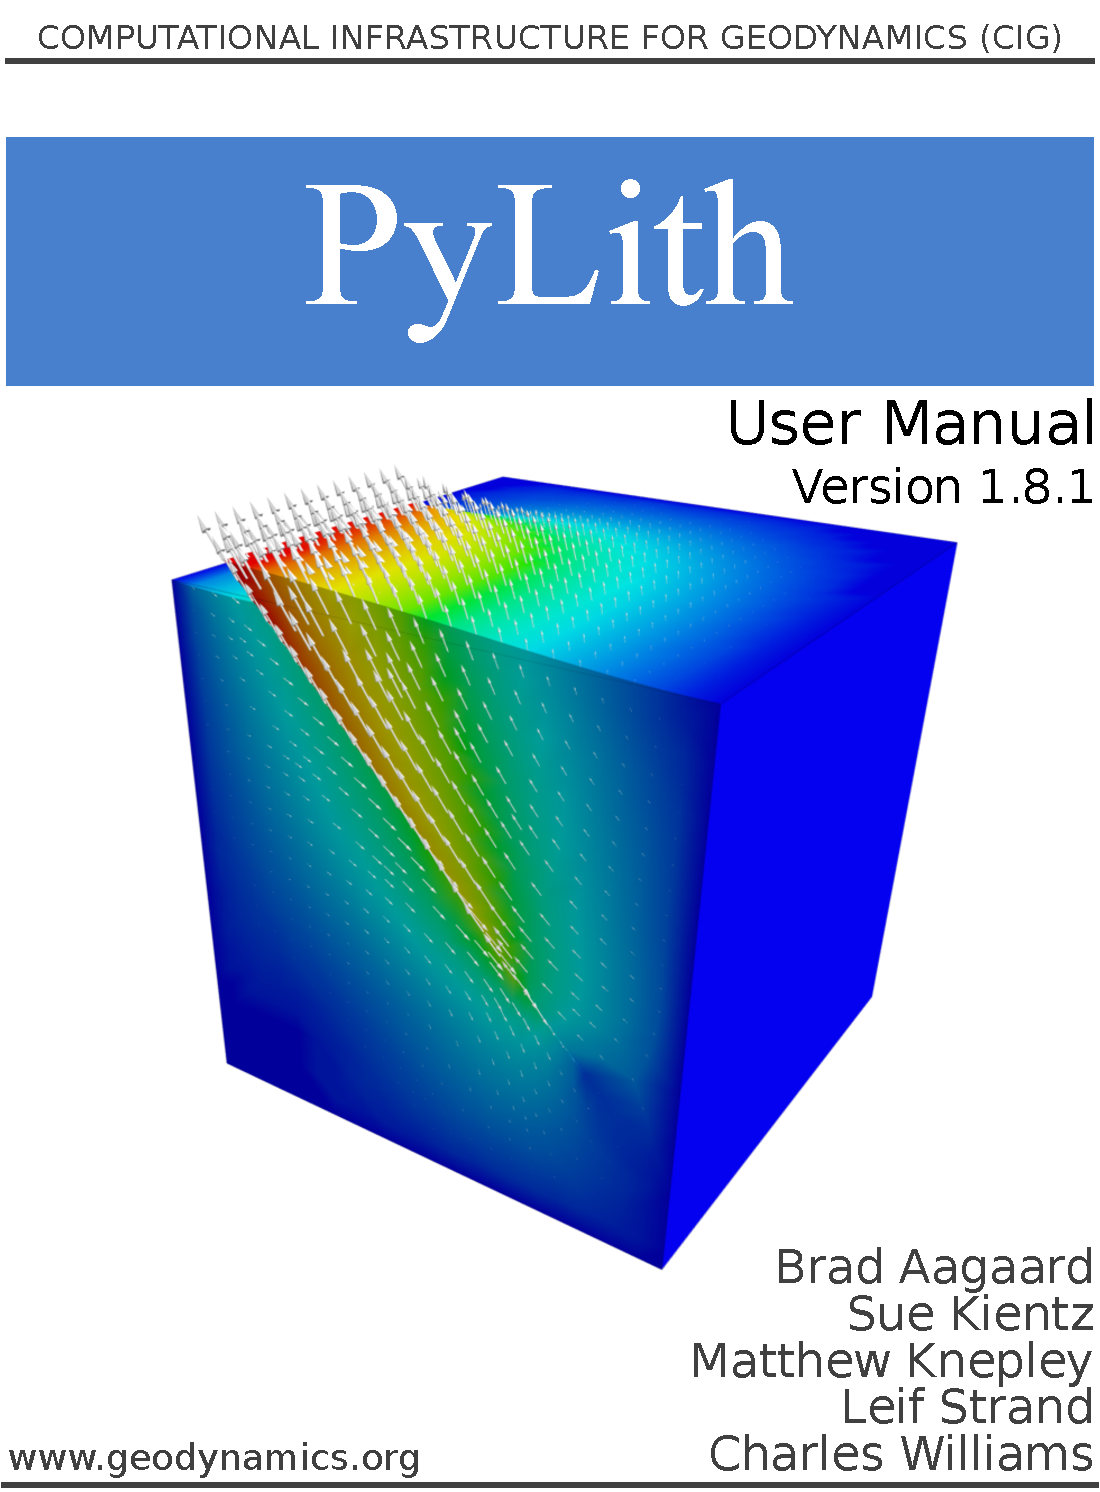
\includegraphics[width=0.75\paperwidth]{cover/cover}
\end{center}
\thispagestyle{empty}

\maketitle

\frontmatter
\tableofcontents{}
\listoffigures
\listoftables


\chapter{Preface}


\section{About This Document}

This document is organized into two parts. The first part begins with
an introduction to PyLith and discusses the types of problems that
PyLith can solve and how to run the software; the second part provides
appendices and references.


\section{Who Will Use This Documentation}

This documentation is aimed at two categories of users: scientists
who prefer to use prepackaged and specialized analysis tools, and
experienced computational Earth scientists. Of the latter, there are
likely to be two classes of users: those who just run models, and
those who modify the source code. Users who modify the source are
likely to have familiarity with scripting, software installation,
and programming, but are not necessarily professional programmers.

\section{Conventions}

\warning{This is a warning.}
\important{This is something important.}
\tip{This is a tip, helpful hint, or suggestion.}

For features recently added to PyLith, we show the version number when
they were added.\newfeature{v2.1.4}

\subsection{Command Line Arguments}

Exmaple of a command line argument: \commandline{-{}-help}.

\subsection{Filenames and Directories}

Example of filenames and directories: \filename{pylith}, \filename{/usr/local}.

\subsection{Unix Shell Commands}

Commands entered into a Unix shell (i.e., terminal) are shown in a
box. Comments are delimited by the \# character. We use 
{\tt \$\$} to indicate the bash shell prompt.
\begin{shell}
# This is a comment.
$$ ls -l
\end{shell}

\subsection{Excerpts of cfg Files}

Exmaple of an excerpt from a \filename{.cfg} file:
\begin{cfg}
# This is a comment.
<h>[pylithapp.problem]</h>
<p>timestep</p> = 2.0*s ; Time step comment.
<f>bc</f> = [x_pos, x_neg]
\end{cfg}

\section{Citation}

The Computational Infrastructure for Geodynamics (CIG) (\url{geodynamics.org})
is making this source code available to you at no cost in hopes that
the software will enhance your research in geophysics. A number of
individuals have contributed a significant portion of their careers
toward the development of this software. It is essential that you
recognize these individuals in the normal scientific practice by citing
the appropriate peer-reviewed papers and making appropriate acknowledgments
in talks and publications. The preferred way to generate the list
of publications (in Bib\TeX{} format) to cite is to run your simulations
with the \commandline{-{}-include-citations} command line argument, or
equivalently, the \commandline{-{}-petsc.citations} command line argument.
The \commandline{-{}-help-citations} command line argument will generate
the Bib\TeX{} entries for the references mentioned below.

The following peer-reviewed paper discussed the development of PyLith:
\begin{itemize}
\item Aagaard, B. T., M. G. Knepley, and C. A. Williams (2013). A domain
decomposition approach to implementing fault slip in finite-element
models of quasi-static and dynamic crustal deformation, \textit{Journal
of Geophysical Research: Solid Earth}, 118, doi: 10.1002/jgrb.50217.
\end{itemize}
To cite this manual, use:
\begin{itemize}
\item Aagaard, B., M. Knepley, C. Williams (2016), \emph{PyLith User Manual,
Version 2.1.4.} Davis, CA: Computational Infrastructure of Geodynamics.\\
URL: geodynamics.org/cig/software/pylith/pylith\_manual-2.1.4.pdf
\end{itemize}

\section{Support}

Current PyLith development is supported by the CIG, and internal GNS
Science \url{www.gns.cri.nz} and U.S. Geological Survey \url{www.usgs.gov}
funding. Pyre development was funded by the Department of Energy's
\url{www.doe.gov/engine/content.do} Advanced Simulation and Computing
program and the National Science Foundation's Information Technology
Research (ITR) program.

This material is based upon work supported by the National Science
Foundation under Grants No. 0313238, 0745391, and EAR-0949446. Any
opinions, findings, and conclusions or recommendations expressed in
this material are those of the author(s) and do not necessarily reflect
the views of the National Science Foundation.


\section{Acknowledgments}

Many members of the community contribute to PyLith through reporting
bugs, suggesting new features and improvements, running benchmarks,
and asking questions about the software. In particular, we thank Surendra
Somala for contributing to the development of the fault friction implementation.


\section{Request for Comments}

Your suggestions and corrections can only improve this documentation.
Please report any errors, inaccuracies, or typos to the CIG Short-Term
Tectonics email list \url{cig-short@geodynamics.org}. 

\mainmatter\raggedbottom


\chapter{Introduction}


\section{Overview}

PyLith is is portable, scalable software for simulation of crustal
deformation across spatial scales ranging from meters to hundreds of
kilometers and temporal scales ranging from milliseconds to thousands
of years. Its primary applications are quasi-static and dynamic
modeling of earthquake faulting.

\section{New in PyLith Version \pylithVersionNumber}
\begin{itemize}
\item Added new examples
  \begin{itemize}
  \item \filename{examples/3d/subduction}: New suite of examples for a 3-D
    subduction zone. This intermediate level suite of examples
    illustrates a wide range of PyLith features for quasi-static simulations.
  \item \filename{examples/2d/subduction}: Added quasi-static spontaneous rupture
    earthquake cycle examples for slip-weakening and rate- and
    state-friction.
  \item These new examples make use of ParaView Python scripts to
    facilitate using ParaView with PyLith.
  \end{itemize}
\item Improved the PyLith manual
  \begin{itemize}
  \item Added diagram to guide users on which installation method best
    meets their needs.
  \item Added instructions for how to use the Windows Subsystem for
    Linux to install the PyLith Linux binary on systems running
    Windows 10.
  \end{itemize}
\item Fixed bug in generating Xdmf files for 2-D vector
  output. Converted Xdmf generator from C++ to Python for more robust
  generation of Xdmf files from Python scripts.
\item Updated spatialdata to v1.9.10. Improved error messages when
  reading SimpleDB and SimpleGridDB files.
\item Updated PyLith parameter viewer to v1.0.1. Small fix to insure
  hierarchy path listed matches the one for PyLith.
\item Updated PETSc to v3.7.6. See the PETSc documentation for a
  summary of all of the changes.
\item Switched to using CentOS 6.9 for Linux binary builds to insure
  compatibility with glibc 2.12 and later.
\end{itemize}
The \filename{CHANGES} file in the top-level source directory contains
a summary of features and bugfixes for each release.


\section{History}

PyLith 1.0 was the first version to allow the solution of both
implicit (quasi-static) and explicit (dynamic) problems and was a
complete rewrite of the original PyLith (version 0.8). PyLith 1.0
combines the functionality of EqSim
\cite{Aagaard:etal:2001a,Aagaard:etal:2001b} and PyLith 0.8. PyLith
0.8 was a direct descendant of LithoMop and was the first version that
ran in parallel, as well as providing several other improvements over
LithoMop. LithoMop was the product of major reengineering of Tecton, a
finite-element code for simulating static and quasi-static crustal
deformation. The major new features present in LithoMop included
dynamic memory allocation and the use of the Pyre simulation framework
and PETSc solvers. EqSim was written by Brad Aagaard to solve problems
in earthquake dynamics, including rupture propagation and seismic wave
propagation.

The release of PyLith 1.0 has been followed by additional releases
that expand the number of features as well as improve performance.
The PyLith 1.x series of releases allows the solution of both
quasi-static and dynamic problems in one, two, or three
dimensions. The code runs in either serial or parallel, and the design
allows for relatively easy scripting using the Python programming
language. Material properties and values for boundary and fault
conditions are specified using spatial databases, which permit easy
prescription of complex spatial variations of properties and
parameters. Simulation parameters are generally specified through the
use of simple ASCII files or the command line.  At present, mesh
information may be provided using a simple ASCII file (PyLith mesh
ASCII format) or imported from CUBIT or LaGriT, two widely-used
meshing packages. The elements currently available include a linear
bar in 1D, linear triangles and quadrilaterals in 2D, and linear
tetrahedra and hexahedra in 3D. Materials presently available include
isotropic elastic, linear Maxwell viscoelastic, generalized Maxwell
viscoelastic, power-law viscoelastic, and Drucker-Prager
elastoplastic. Boundary conditions include Dirichlet (prescribed
displacements and velocities), Neumann (traction), point forces, and
absorbing boundaries.  Cohesive elements are used to implement slip
across interior surfaces (faults) with both kinematically-specified
fault slip and slip governed by fault constitutive models. PyLith also
includes an interface for computing static Green's functions for fault
slip.

PyLith 2.0 replaces the finite-element data structures provided by the
C++ Sieve implementation with those provided by the C DMPlex
implementation.  The newly developed DMPlex implementation by the
PETSc developers conforms to the PETSc data manager (DM) interface,
thereby providing tighter integration with other PETSc data
structures, such as vectors and matrices. Other improvements include
significantly reduced memory use and memory balancing.

PyLith is under active development and we expect a number of additions
and improvements in the near future. Likely enhancements will include
additional bulk and fault constitutive models, coupled quasi-static
and dynamic simulations for earthquake cycle modeling, and coupling
between elasticity, heat flow, and/or fluid flow.


\section{PyLith Workflow}

PyLith is one component in the process of investigating problems in
tectonics (Figure \vref{fig:Workflow-summary}). Given a geological
problem of interest, a scientist must first provide a geometrical
representation of the desired structure. Once the structure has been
defined, a computational mesh must be created. PyLith presently
provides three mesh importing options: CUBIT Exodus format, LaGriT GMV
and Pset files, and PyLith mesh ASCII format. The modeling of the
physical processes of interest is performed by a code such as
PyLith. Present output consists of VTK or HDF5/Xdmf files which can be
used by a number of visualization codes (e.g., ParaView, Visit, and
Matlab).

\begin{figure}[htbp]
  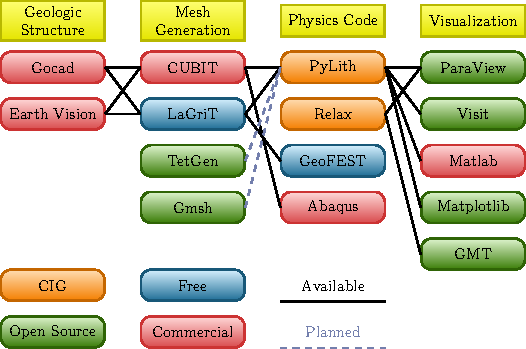
\includegraphics[width=4in]{intro/figs/workflow}
  \caption{Workflow involved in going from geologic structure to
    problem analysis.}
  \label{fig:Workflow-summary}
\end{figure}

\section{PyLith Design}

PyLith is separated into modules to encapsulate behavior and facilitate
use across multiple applications. This allows expert users to replace
functionality of a wide variety of components without recompiling
or polluting the main code. PyLith employs external packages (see
Figure \vref{fig:pylith-dependencies}) to reduce development time
and enhance computational efficiency; for example, PyLith 0.8 ran
two times faster when the PETSc linear solver was used.

\begin{figure}[htbp]
  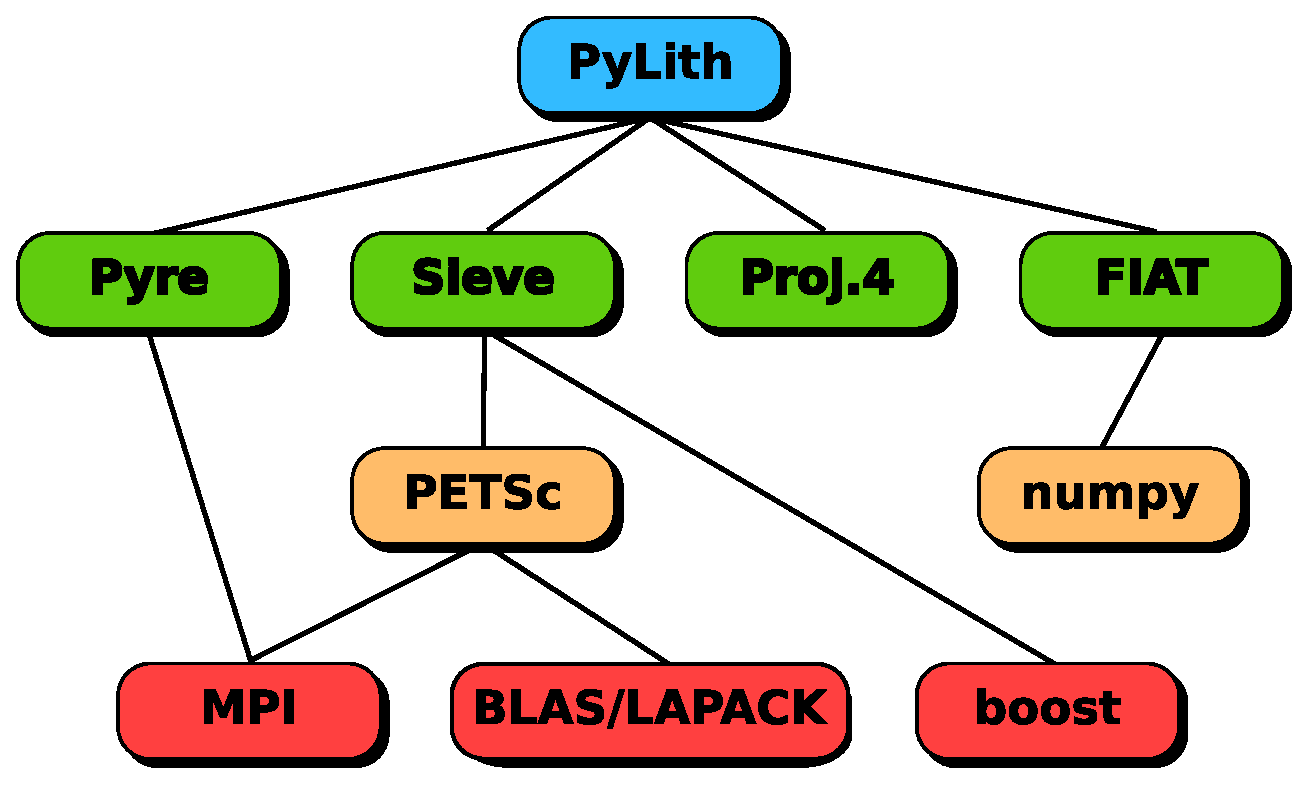
\includegraphics[width=4in]{intro/figs/packages}
  \caption{PyLith dependencies. PyLith makes direct use of several
    other packages, some of which have their own dependencies.}
  \label{fig:pylith-dependencies}
\end{figure}

PyLith is written in two programming languages. High-level code is
written in Python; this rich, expressive interpreted language with
dynamic typing reduces development time and permits flexible addition
of user-contributed modules. This high-level code makes use of Pyre, a
science-neutral simulation framework developed at Caltech, to link the
modules together at runtime and gather user-input. Low-level code is
written in C++, providing fast execution while still allowing an
object-oriented implementation. This low-level code relies on PETSc to
perform operations on matrices and vectors in parallel. We also make
extensive use of two Python packages. SWIG is a package that
simplifies the task of adding C++ extensions to Python code, and FIAT
provides tabulated basis functions and numerical quadrature points.

In writing PyLith 1.0, the code was designed to be object-oriented and
modular. Each type of module is accessed through a specified interface
(set of functions). This permits adding, replacing, and rewriting
modules without affecting other parts of the code. This code structure
simplifies code maintenance and development. Extending the set of code
features is also easier, since developers can create new modules
derived from the existing ones.

The current code design leverages Pyre and PETSc extensively. Pyre
glues together the various modules used to construct a simulation and
specify the parameters. PETSc provides the finite-element data
structures and handles the creation and manipulation of matrices and
vectors. As a result, most of the PyLith source code pertains to
implementing the geodynamics, such as bulk rheology, boundary
conditions, and slip on faults.

PyLith also uses FIAT to tabulate the finite-element basis functions
at the numerical integration (quadrature) points. Nemesis allows
PyLith to run Python using the Message Passing Interface (MPI) for
parallel processing. Additional, indirect dependencies (see Figure
\vref{fig:pylith-dependencies}) include numpy (efficient operations on
numerical arrays in Python), Proj.4 (geographic projections), and SWIG
(calling C++ functions from Python).

During development, tests were constructed for nearly every module
function. These unit tests are distributed with the source code. These
tests are run throughout the development cycle to expose bugs and
isolate their origin. As additional changes are made to the code, the
tests are rerun to help prevent introduction of new bugs. A number of
simple, full-scale tests, such as axial compression and extension,
simple shear, and slip on through-going faults, have been used to test
the code. Additionally, we have run the Southern California Earthquake
Center crustal deformation and several of the spontaneous rupture
benchmarks for strike-slip and reverse-slip to determine the relative
local and global error (see Chapter \vref{sec:benchmarks}).

\subsection{Pyre}

Pyre is an object-oriented environment capable of specifying and launching
numerical simulations on multiple platforms, including Beowulf-class
parallel computers and grid computing systems. Pyre allows the binding
of multiple components such as solid and fluid models used in Earth
science simulations, and different meshers. The Pyre framework enables
the elegant setup, modification and launching of massively parallel
solver applications.

\begin{figure}[htbp]
  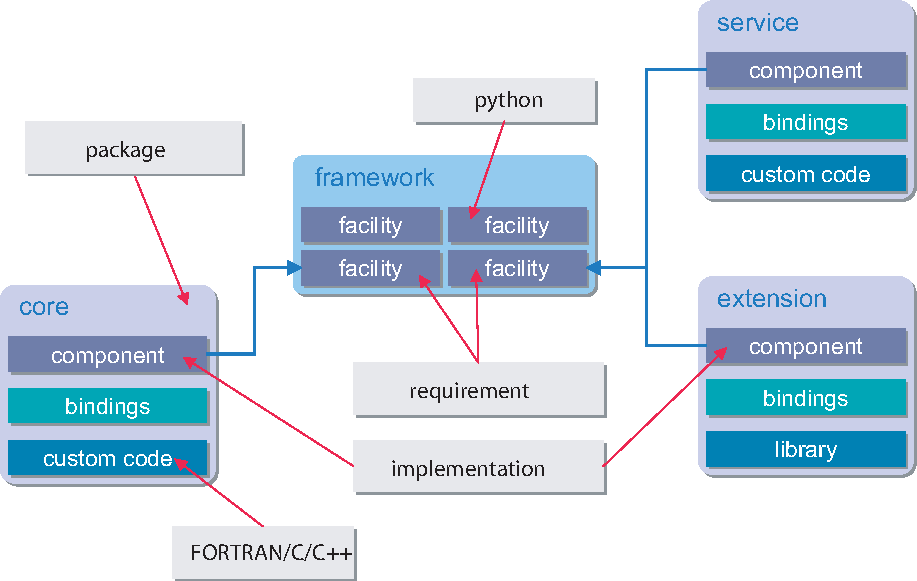
\includegraphics[width=4in]{intro/figs/pyre_overview}
  \caption{Pyre Architecture. The integration framework is a set of
    cooperating abstract services.}
  \label{fig:Pyre:Architecture}
\end{figure}

Pyre is a framework, a combination of software and design philosophy
that promotes the reuse of code. In their canonical software design
book, \emph{Design Patterns}, Erich Gamma \textit{et al}. condense
the concept of a framework concept down to, ``When you use a framework,
you reuse the main body and write the code it calls.'' In the context
of frameworks and object-oriented programming, Pyre can be thought
of as a collection of classes and the way their instances interact.
Programming applications based on Pyre will look similar to those
written in any other object-oriented language. The Pyre framework
contains a subset of parts that make up the overall framework. Each
of those parts is designed to solve a specific problem.

The framework approach to computation offers many advantages. It permits
the exchange of codes and promotes the reuse of standardized software
while preserving efficiency. Frameworks are also an efficient way
to handle changes in computer architecture. They present programmers
and scientists with a unified and well-defined task and allow for
shared costs of the housekeeping aspects of software development.
They provide greater institutional continuity to model development
than piecemeal approaches.

The Pyre framework incorporates features aimed at enabling the
scientific non-expert to perform tasks easily without hindering the
expert. Target features for end users allow complete and intuitive
simulation specification, reasonable defaults, consistency checks of
input, good diagnostics, easy access to remote facilities, and status
monitoring. Target features for developers include easy access to user
input, a shorter development cycle, and good debugging support.


\subsection{PETSc}

PyLith 2.x makes use of a set of data structures and routines in PETSc
called \object{DMPlex}, which is still under active
development. \object{DMPlex} provides data structures and routines for
for representing and manipulating computational meshes, and it greatly
simplifies finite-element computations.\object{DMPlex} represents the
topology of the domain. Zero volume elements are inserted along all
fault surfaces to implement kinematic (prescribed) or dynamic
(constitutive model) implementations of fault slip. Material
properties and other parameters are represented as scalar and vector
fields over the mesh using vectors to store the values and sections to
map vertices, edges, faces, and cells to indices in the vector. For
each problem, functions are provided to calculate the residual and its
Jacobian.  All numerical integration is done in these functions, and
parallel assembly is accomplished using the get/set closure paradigm
of the \object{DMPlex} framework. We assemble into PETSc linear
algebra objects and then call PETSc solvers.

PETSc \url{www-unix.mcs.anl.gov/petsc/petsc-as}, the Portable,
Extensible Toolkit for Scientific computation, provides a suite of
routines for parallel, numerical solution of partial differential
equations for linear and nonlinear systems with large, sparse systems
of equations.  PETSc includes solvers that implement a variety of
Newton and Krylov subspace methods. It can also interface with many
external packages, including ESSL, MUMPS, Matlab, ParMETIS, PVODE, and
Hypre, thereby providing additional solvers and interaction with other
software packages.

PETSc includes interfaces for FORTRAN 77/90, C, C++, and Python for
nearly all of the routines, and PETSc can be installed on most Unix
systems. PETSc can be built with user-supplied, highly optimized
linear algebra routines (e.g., ATLAS and commercial versions of
BLAS/LAPACK), thereby improving application performance. Users can use
PETSc parallel matrices, vectors, and other data structures for most
parallel operations, eliminating the need for explicit calls to
Message Passing Interface (MPI) routines. Many settings and options
can be controlled with PETSc-specific command-line arguments,
including selection of preconditions, solvers, and generation of
performance logs.

\chapter{Governing Equations}
\label{cha:governing:equations}

We present here a brief derivation of the equations for both quasi-static
and dynamic computations. Since the general equations are the same
(except for the absence of inertial terms in the quasi-static case),
we first derive these equations. We then present solution methods
for each specific case. In all of our derivations, we use the notation
described in Table \vref{tab:notation} for both index
and vector notation. When using index notation, we use the common
convention that repeated indices indicate summation over the range
of the index.

\begin{table}[htbp]
\caption{Mathematical notation}
\label{tab:notation}

\begin{tabular}{|c|c|c|}
\hline 
\multicolumn{2}{|c|}{Symbol} & Description\tabularnewline
\cline{1-2} 
Index notation & Vector Notation & \tabularnewline
\hline 
\hline 
$a_{i}$ & $\overrightarrow{a}$ & Vector field a\tabularnewline
\hline 
$a_{ij}$ & $\underline{a}$ & Second order tensor field a\tabularnewline
\hline 
$u_{i}$ & $\overrightarrow{u}$ & Displacement vector field\tabularnewline
\hline 
$d_{i}$ & $\vec{{d}}$ & Fault slip vector field\tabularnewline
\hline 
$f_{i}$ & $\overrightarrow{f}$ & Body force vector field\tabularnewline
\hline 
$T_{i}$ & $\overrightarrow{T}$ & Traction vector field\tabularnewline
\hline 
$\sigma_{ij}$ & $\underline{\sigma}$ & Stress tensor field\tabularnewline
\hline 
$n_{i}$ & $\overrightarrow{n}$ & Normal vector field\tabularnewline
\hline 
$\rho$ & $\rho$ & Mass density scalar field\tabularnewline
\hline 
\end{tabular}
\end{table}


\section{Derivation of Elasticity Equation}


\subsection{Index Notation}

Consider volume $V$ bounded by surface $S$. Applying a Lagrangian
description of the conservation of momentum gives

\begin{equation}
\frac{\partial}{\partial t}\int_{V}\rho\frac{\partial u_{i}}{\partial t}\, dV=\int_{V}f_{i}\, dV+\int_{S}T_{i}\, dS.\label{eqn:momentum:index}
\end{equation}
The traction vector field is related to the stress tensor through
\begin{equation}
T_{i}=\sigma_{ij}n_{j},
\end{equation}
where $n_{j}$ is the vector normal to $S$. Substituting into equation
\vref{eqn:momentum:index} yields
\begin{equation}
\frac{\partial}{\partial t}\int_{V}\rho\frac{\partial u_{i}}{\partial t}\, dV=\int_{V}f_{i}\, dV+\int_{S}\sigma_{ij}n_{j}\, dS.
\end{equation}
Applying the divergence theorem,
\begin{equation}
\int_{V}a_{i,j}\: dV=\int_{S}a_{j}n_{j}\: dS,
\end{equation}
to the surface integral results in
\begin{equation}
\frac{\partial}{\partial t}\int_{V}\rho\frac{\partial u_{i}}{\partial t}\, dV=\int_{V}f_{i}\, dV+\int_{V}\sigma_{ij,j}\, dV,
\end{equation}
which we can rewrite as
\begin{equation}
\int_{V}\left(\rho\frac{\partial^{2}u_{i}}{\partial t^{2}}-f_{i}-\sigma_{ij,j}\right)\, dV=0.
\end{equation}
Because the volume $V$ is arbitrary, the integrand must be zero at
every location in the volume, so that we end up with
\begin{gather}
\rho\frac{\partial^{2}u_{i}}{\partial t^{2}}-f_{i}-\sigma_{ij,j}=0\text{ in }V,\\
\sigma_{ij}n_{j}=T_{i}\text{ on }S_{T}\text{,}\\
u_{i}=u_{i}^{o}\text{ on }S_{u}\text{, and}\\
R_{ki}(u_{i}^{+}-u_{i}^{-})=d_{k}\text{ on }S_{f}.
\end{gather}
We specify tractions, $T_{i}$, on surface $S_{f}$, displacements,
$u_{i}^{o}$, on surface $S_{u}$, and slip, $d_{k}$, on fault surface
$S_{f}$ (we will consider the case of fault constitutive models in
Section \vref{sec:fault}). The rotation matrix $R_{ki}$ transforms
vectors from the global coordinate system to the fault coordinate
system. Note that since both $T_{i}$ and $u_{i}$ are vector quantities,
there can be some spatial overlap of the surfaces $S_{T}$ and $S_{u}$;
however, the same degree of freedom cannot simultaneously have both
types of boundary conditions.


\subsection{Vector Notation}

Consider volume $V$ bounded by surface $S$. Applying a Lagrangian
description of the conservation of momentum gives

\begin{equation}
\frac{\partial}{\partial t}\int_{V}\rho\frac{\partial\vec{u}}{\partial t}\, dV=\int_{V}\overrightarrow{f}\, dV+\int_{S}\overrightarrow{T}\, dS.\label{eqn:momentum:vec}
\end{equation}
The traction vector field is related to the stress tensor through
\begin{equation}
\overrightarrow{T}=\underline{\sigma}\cdot\overrightarrow{n},
\end{equation}
where $\overrightarrow{n}$ is the vector normal to $S$. Substituting
into equation \vref{eqn:momentum:vec} yields
\begin{equation}
\frac{\partial}{\partial t}\int_{V}\rho\frac{\partial\overrightarrow{u}}{\partial t}\, dV=\int_{V}\overrightarrow{f}\, dV+\int_{S}\underline{\sigma}\cdot\overrightarrow{n}\, dS.
\end{equation}
Applying the divergence theorem,
\begin{equation}
\int_{V}\nabla\cdot\overrightarrow{a}\: dV=\int_{S}\overrightarrow{a}\cdot\overrightarrow{n}\: dS,
\end{equation}
to the surface integral results in
\begin{equation}
\frac{\partial}{\partial t}\int_{V}\rho\frac{\partial\overrightarrow{u}}{\partial t}\, dV=\int_{V}\overrightarrow{f}\, dV+\int_{V}\nabla\cdot\underline{\sigma}\, dV,
\end{equation}
which we can rewrite as
\begin{equation}
\int_{V}\left(\rho\frac{\partial^{2}\overrightarrow{u}}{\partial t^{2}}-\overrightarrow{f}-\nabla\cdot\overrightarrow{\sigma}\right)\, dV=\vec{0}.
\end{equation}
Because the volume $V$ is arbitrary, the integrand must be the zero
vector at every location in the volume, so that we end up with
\begin{gather}
\rho\frac{\partial^{2}\overrightarrow{u}}{\partial t^{2}}-\overrightarrow{f}-\nabla\cdot\overrightarrow{\sigma}=\vec{0}\text{ in }V,\\
\underline{\sigma}\cdot\overrightarrow{n}=\overrightarrow{T}\text{ on }S_{T}\text{,}\\
\overrightarrow{u}=\overrightarrow{u^{o}}\text{ on }S_{u},\text{ and}\\
\underbar{R}\cdot(\vec{u^{+}}-\vec{u^{-}})=\vec{d}\text{ on }S_{f}.
\end{gather}
We specify tractions, $\vec{T}$, on surface $S_{f}$, displacements,
$\overrightarrow{u^{o}}$, on surface $S_{u}$, and slip, $\vec{d}$,
on fault surface $S_{f}$ (we will consider the case of fault constitutive
models in Section \vref{sec:fault}). The rotation matrix $\underline{R}$
transforms vectors from the global coordinate system to the fault
coordinate system. Note that since both $\overrightarrow{T}$ and
$\overrightarrow{u}$ are vector quantities, there can be some spatial
overlap of the surfaces $S_{T}$ and $S_{u}$; however, the same degree
of freedom cannot simultaneously have both types of boundary conditions.


\section{Finite-Element Formulation of Elasticity Equation}

We formulate a set of algebraic equations using Galerkin's method.
We consider (1) a trial solution, $\vec{u}$, that is a piecewise
differentiable vector field and satisfies the Dirichlet boundary conditions
on $S_{u}$, and (2) a weighting function, $\vec{\phi}$, that is
a piecewise differentiable vector field and is zero on $S_{u}$.


\subsection{Index Notation}

We start with the wave equation (strong form),

\begin{gather}
\sigma_{ij,j}+f_{i}=\rho\ddot{u_{i}}\text{ in }V,\\
\sigma_{ij}n_{j}=T_{i}\text{ on }S_{T},\\
u_{i}=u_{i}^{o}\text{ on }S_{u},\\
R_{ki}(u_{i}^{+}-u_{i}^{-})=d_{k}\text{ on }S_{f},\text{ and}\\
\sigma_{ij}=\sigma_{ji}\text{ (symmetric).}
\end{gather}
We construct the weak form by computing the dot product of the wave
equation and weighting function and setting the integral over the
domain to zero:
\begin{gather}
\int_{V}\left(\sigma_{ij,j}+f_{i}-\rho\ddot{u}_{i}\right)\phi_{i}\, dV=0\text{, or }\\
\int_{V}\sigma_{ij,j}\phi_{i}\: dV+\int_{V}f_{i}\phi_{i}\: dV-\int_{V}\rho\ddot{u}_{i}\phi_{i}\: dV=0.
\end{gather}
 Consider the divergence theorem applied to the dot product of the
stress tensor and the weighting function, $\sigma_{ij}\phi_{i}$,
\begin{equation}
\int_{V}(\sigma_{ij}\phi_{i})_{,j}\, dV=\int_{S}(\sigma_{ij}\phi_{i})n_{i}\, dS.
\end{equation}
Expanding the left-hand side yields
\begin{gather}
\int_{V}\sigma_{ij,j}\phi_{i}\: dV+\int_{V}\sigma_{ij}\phi_{i,j}\: dV=\int_{S}\sigma_{ij}\phi_{i}n_{i}\: dS,\text{ or}\\
\int_{V}\sigma_{ij,j}\phi_{i}\: dV=-\int_{V}\sigma_{ij}\phi_{i,j}\, dV+\int_{S}\sigma_{ij}\phi_{i}n_{i}\, dS.
\end{gather}
Substituting into the weak form gives
\begin{equation}
-\int_{V}\sigma_{ij}\phi_{i,j}\, dV+\int_{S}\sigma_{ij}\phi_{i}n_{i}\, dS+\int_{V}f_{i}\phi_{i}\, dV-\int_{V}\rho\ddot{u}_{i}\phi_{i}\, dV=0.
\end{equation}
Turning our attention to the second term, we separate the integration
over $S$ into integration over $S_{T}$ and $S_{u}$ (we will consider
tractions over the fault surface, $S_{f}$, associated with the fault
constitutive model in Section \vref{sec:fault}),
\begin{equation}
-\int_{V}\sigma_{ij}\phi_{i,j}\, dV+\int_{S_{T}}\sigma_{ij}\phi_{i}n_{i}\, dS+\int_{S_{u}}\sigma_{ij}\phi_{i}n_{i}\, dS+\int_{V}f_{i}\phi_{i}\, dV-\int_{V}\rho\ddot{u}_{i}\phi_{i}\, dV=0,
\end{equation}
and recognize that
\begin{gather}
\sigma_{ij}n_{i}=T_{i}\text{ on }S_{T}\text{ and}\\
\phi_{i}=0\text{ on }S_{u},
\end{gather}
so that the equation reduces to
\begin{equation}
-\int_{V}\sigma_{ij}\phi_{i,j}\: dV+\int_{S_{T}}T_{i}\phi_{i}\, dS+\int_{V}f_{i}\phi_{i}\, dV-\int_{V}\rho\ddot{u}_{i}\phi_{i}\, dV=0.\label{eq:elasticity:integral}
\end{equation}
We express the trial solution and weighting function as linear combinations
of basis functions,
\begin{gather}
u_{i}=\sum_{m}a_{i}^{m}N^{m},\\
\phi_{i}=\sum_{n}c_{i}^{n}N^{n}.
\end{gather}
Note that because the trial solution satisfies the Dirichlet boundary
condition, the number of basis functions for $u$ is generally greater
than the number of basis functions for $\phi$, i.e., $m>n$. Substituting
in the expressions for the trial solution and weighting function yields
\begin{gather}
-\int_{V}\sigma_{ij}\sum_{n}c_{i}^{n}N_{,j}^{n}\: dV+\int_{S_{T}}T_{i}\sum_{n}c_{i}^{n}N^{n}\, dS+\int_{V}f_{i}\sum_{n}c_{i}^{n}N^{n}\, dV-\int_{V}\rho\sum_{m}\ddot{a}_{i}^{m}N^{m}\sum_{n}c_{i}^{n}N^{n}\ dV=0,\text{ or}\\
\sum_{n}c_{i}^{n}(-\int_{V}\sigma_{ij}N_{,j}^{n}\: dV+\int_{S_{T}}T_{i}N^{n}\, dS+\int_{V}f_{i}N^{n}\, dV-\int_{V}\rho\sum_{m}\ddot{a}_{i}^{m}N^{m}N^{n}\ dV)=0.
\end{gather}
 Because the weighting function is arbitrary, this equation must hold
for all $c_{i}^{n}$, so that the quantity in parenthesis is zero
for each $c_{i}^{n}$
\begin{equation}
-\int_{V}\sigma_{ij}N_{,j}^{n}\: dV+\int_{S_{T}}T_{i}N^{n}\, dS+\int_{V}f_{i}N^{n}\, dV-\int_{V}\rho\sum_{m}\ddot{a}_{i}^{m}N^{m}N^{n}\ dV=\vec{0}.\label{eq:elasticity:integral:discretized}
\end{equation}
We want to solve this equation for the unknown coefficients $a_{i}^{m}$
subject to

\begin{gather}
u_{i}=u_{i}^{o}\text{ on }S_{u},\text{ and}\\
R_{ki}(u_{i}^{+}-u_{i}^{-})=d_{k}\text{ on }S_{f},
\end{gather}



\subsection{Vector Notation}

We start with the wave equation (strong form),

\begin{gather}
\nabla\cdot\underline{\sigma}+\overrightarrow{f}=\rho\frac{\partial^{2}\overrightarrow{u}}{\partial t^{2}}\text{ in }V,\\
\underline{\sigma}\cdot\overrightarrow{n}=\overrightarrow{T}\text{ on }S_{T},\\
\overrightarrow{u}=\overrightarrow{u^{o}}\text{ on }S_{u},\\
\underbar{R}\cdot(\overrightarrow{u^{+}}-\overrightarrow{u^{-}})=\vec{d}\text{ on }S_{f}\\
\underline{\sigma}=\underline{\sigma}^{T}\text{ (symmetric).}
\end{gather}
We construct the weak form by multiplying the wave equation by a weighting
function and setting the integral over the domain to zero. The weighting
function is a piecewise differential vector field, $\overrightarrow{\phi}$,
where $\overrightarrow{\phi}=0$ on $S_{u}.$ Hence our weak form
is
\begin{gather}
\int_{V}\left(\nabla\cdot\underline{\sigma}+\overrightarrow{f}-\rho\frac{\partial^{2}\overrightarrow{u}}{\partial t^{2}}\right)\cdot\overrightarrow{\phi}\, dV=0\text{, or }\\
\int_{V}(\nabla\cdot\underline{\sigma})\cdot\overrightarrow{\phi}\: dV+\int_{V}\overrightarrow{f}\cdot\overrightarrow{\phi}\: dV-\int_{V}\rho\frac{\partial^{2}\overrightarrow{u}}{\partial t^{2}}\cdot\overrightarrow{\phi}\: dV=0.
\end{gather}
 Consider the divergence theorem applied to the dot product of the
stress tensor and the trial function, $\underline{\sigma}\cdot\overrightarrow{\phi}$,
\begin{equation}
\int_{V}\nabla\cdot(\underline{\sigma}\cdot\overrightarrow{\phi})\, dV=\int_{S}(\underline{\sigma}\cdot\overrightarrow{\phi})\cdot\overrightarrow{n}\, dS.
\end{equation}
Expanding the left-hand side yields
\begin{equation}
\int_{V}(\nabla\cdot\underline{\sigma})\cdot\overrightarrow{\phi}\: dV+\int_{V}\underline{\sigma}:\nabla\overrightarrow{\phi}\: dV=\int_{S}(\underline{\sigma}\cdot\overrightarrow{\phi})\cdot\overrightarrow{n}\: dS,\text{ or}
\end{equation}
\begin{equation}
\int_{V}(\nabla\cdot\underline{\sigma})\cdot\overrightarrow{\phi}\: dV=-\int_{V}\underline{\sigma}:\nabla\overrightarrow{\phi}\, dV+\int_{S}\underline{\sigma}\cdot\overrightarrow{n}\cdot\overrightarrow{\phi}\, dS.
\end{equation}
Substituting into the weak form gives
\begin{equation}
-\int_{V}\underline{\sigma}:\nabla\overrightarrow{\phi}\, dV+\int_{S}\underline{\sigma}\cdot\overrightarrow{n}\cdot\overrightarrow{\phi}\, dS+\int_{V}\overrightarrow{f}\cdot\overrightarrow{\phi}\, dV-\int_{V}\rho\frac{\partial^{2}\overrightarrow{u}}{\partial t^{2}}\cdot\overrightarrow{\phi}\, dV=0.
\end{equation}
We separate the integration over $S$ into integration over $S_{T}$
and $S_{u}$,
\begin{multline}
-\int_{V}\underline{\sigma}:\nabla\overrightarrow{\phi}\, dV+\int_{S_{T}}\underline{\sigma}\cdot\overrightarrow{n}\cdot\overrightarrow{\phi}\, dS+\int_{S_{u}}\underline{\sigma}\cdot\overrightarrow{n}\cdot\overrightarrow{\phi}\, dS+\int_{V}\overrightarrow{f}\cdot\overrightarrow{\phi}\, dV-\int_{V}\rho\frac{\partial^{2}\overrightarrow{u}}{\partial t^{2}}\cdot\overrightarrow{\phi}\, dV=0,
\end{multline}
and recognize that
\begin{gather}
\underline{\sigma}\cdot\overrightarrow{n}=\overrightarrow{T}\text{ on }S_{T}\text{ and}\\
\overrightarrow{\phi}=0\text{ on }S_{u},
\end{gather}
so that the equation reduces to
\begin{equation}
-\int_{V}\underline{\sigma}:\nabla\overrightarrow{\phi}\: dV+\int_{S_{T}}\overrightarrow{T}\cdot\overrightarrow{\phi}\, dS+\int_{V}\overrightarrow{f}\cdot\overrightarrow{\phi}\, dV-\int_{V}\rho\frac{\partial^{2}\overrightarrow{u}}{\partial t^{2}}\cdot\overrightarrow{\phi}\, dV=0.
\end{equation}
We express the trial solution and weighting function as linear combinations
of basis functions,
\begin{gather}
\vec{u}=\sum_{m}\overrightarrow{a^{m}}N^{m},\\
\vec{\phi}=\sum_{n}\overrightarrow{c^{n}}N^{n}.
\end{gather}
Note that because the weighting function is zero on $S_{u}$, the
number of basis functions for $\vec{u}$ is generally greater than
the number of basis functions for $\vec{\phi}$, i.e., $m>n$. Substituting
in the expressions for the trial solution and weighting function yields
\begin{multline}
-\int_{V}\underline{\sigma}:\sum_{n}\overrightarrow{c^{n}}\nabla N_{,}^{n}\, dV+\int_{S_{T}}\vec{T}\cdot\sum_{n}\overrightarrow{c^{n}}N^{n}\, dS+\int_{V}\vec{f}\cdot\sum_{n}\overrightarrow{c^{n}}N^{n}\, dV\\
-\int_{V}\rho\sum_{m}\frac{\partial^{2}\overrightarrow{a^{m}}}{\partial t^{2}}N^{m}\cdot\sum_{n}\overrightarrow{c^{n}}N^{n}\ dV=0.
\end{multline}
 Because the weighting function is arbitrary, this equation must hold
for all $\overrightarrow{c^{n}}$, so that
\begin{equation}
-\int_{V}\underline{\sigma}:\nabla N^{n}\, dV+\int_{S_{T}}\vec{T}N^{n}\, dS+\int_{V}\vec{f}N^{n}\, dV-\int_{V}\rho\sum_{m}\frac{\partial^{2}\overrightarrow{a^{m}}}{\partial t^{2}}N^{m}N^{n}\, dV=\vec{0}.
\end{equation}
We want to solve this equation for the unknown coefficients $\overrightarrow{a^{m}}$
subject to

\begin{gather}
\vec{u}=u^{o}\overrightarrow{}\text{ on }S_{u},\text{ and}\\
\underline{R}(\overrightarrow{u^{+}}-\overrightarrow{u^{-}})=\vec{d}\text{ on }S_{f},
\end{gather}



\section{Solution Method for Quasi-Static Problems}

For brevity we outline the solution method for quasi-static problems
using only index notation. In quasi-static problems we neglect the
inertial terms, so equation \eqref{eq:elasticity:integral:discretized}
reduces to
\begin{equation}
-\int_{V}\sigma_{ij}N_{,j}^{n}\: dV+\int_{S_{T}}T_{i}N^{n}\, dS+\int_{V}f_{i}N^{n}\, dV=\vec{0}.
\end{equation}
As a result, time-dependence only enters through the constitutive
relationships and the loading conditions. We consider the deformation
at time $t+\Delta t$,
\begin{equation}
-\int_{V}\sigma_{ij}(t+\Delta t)N_{,j}^{n}\: dV+\int_{S_{T}}T_{i}(t+\Delta t)N^{n}\, dS+\int_{V}f_{i}(t+\Delta t)N^{n}\, dV=\vec{0}.\label{eq:elasticity:integral:quasistatic}
\end{equation}
We solve this equation through formulation of a linear algebraic system
of equations ($Au=b$), involving the residual ($r=b-Au$) and Jacobian
($A$). The residual is simply
\begin{equation}
r_{i}^{n}=-\int_{V}\sigma_{ij}(t+\Delta t)N_{,j}^{n}\: dV+\int_{S_{T}}T_{i}(t+\Delta t)N^{n}\, dS+\int_{V}f_{i}(t+\Delta t)N^{n}\, dV.
\end{equation}
We employ numerical quadrature in the finite-element discretization
and replace the integrals with sums over the cells and quadrature
points,
\begin{multline}
r_{i}^{n}=-\sum_{\text{vol cells}}\sum_{\text{quad pts}}\sigma_{ij}(x_{q},t+\Delta t)N_{,j}^{n}(x_{q})\: w_{q}|J_{cell}(x_{q})|+\sum_{\text{vol cells}}\sum_{\text{quad pt}s}f_{i}(x_{q},t+\Delta t)N^{n}(x_{q})\, w_{q}|J_{cell}(x_{q})|\\
+\sum_{\text{tract cells}}\sum_{\text{quad pts}}T_{i}(x_{q},t+\Delta t)N^{n}(x_{q})\, w_{q}|J_{cell}(x_{q})|,
\end{multline}
where $r_{i}^{n}$ is an $nd$ vector ($d$ is the dimension of the
vector space) and $i$ is a vector space component, $x_{q}$ are the
coordinates of the quadrature points, $w_{q}$ are the weights of
the quadrature points, and $|J_{cell}(x_{q})|$ is the determinant
of the Jacobian matrix evaluated at the quadrature points associated
with mapping the vreference cell to the actual cell. The quadrature
scheme for the integral over the tractions is one dimension lower
than the one used in integrating the terms for the volume cells.

In order to find the Jacobian of the system, we let
\begin{equation}
\sigma_{ij}(t+\Delta t)=\sigma_{ij}(t)+d\sigma_{ij}(t).
\end{equation}
Isolating the term associated with the increment in stresses yields

\begin{equation}
\int_{V}d\sigma_{ij}(t)N_{j}^{n}\ dV=-\int_{V}\sigma_{ij}(t)N_{,j}^{n}\: dV+\int_{S_{T}}T_{i}(t+\Delta t)N^{n}\, dS+\int_{V}f_{i}(t+\Delta t)N^{n}\, dV
\end{equation}
We associate the term on the left-hand-side with the action of the
system Jacobian on the increment of the displacement field. We approximate
the increment in stresses using linear elasticity and infinitesimal
strains,

\begin{gather}
d\sigma_{ij}(t)=C_{ijkl}(t)d\varepsilon_{kl}(t)\\
d\sigma_{ij}(t)=\frac{1}{2}C_{ijkl}(t)(du_{k.l}(t)+du_{l,k}(t))\\
d\sigma_{ij}(t)=\frac{1}{2}C_{ijkl}(t)(\sum_{m}da_{k,l}^{m}(t)N^{m}+\sum_{m}da_{l,k}^{m}(t)N^{m})
\end{gather}
Now, $d\sigma_{ij}\phi_{i,j}$ is a scalar, so it is symmetric,
\begin{equation}
d\sigma_{ij}\phi_{i,j}=d\sigma_{ji}\phi_{j,i},
\end{equation}
and we know that $d\sigma_{ij}$ is symmetric, so
\begin{equation}
d\sigma_{ij}\phi_{i,j}=d\sigma_{ij}\phi_{j,i},
\end{equation}
which means
\begin{equation}
\phi_{i,j}=\phi_{j,i},
\end{equation}
which we can write as
\begin{equation}
\phi_{i,j}=\frac{1}{2}(\phi_{i,j}+\phi_{j,i}).
\end{equation}
In terms of the basis functions, we have

\begin{equation}
\sum_{n}c_{i}^{n}N_{,j}^{n}=\frac{1}{2}(\sum_{n}c_{i}^{n}N_{,j}^{n}+\sum_{n}c_{j}^{n}N_{,i}^{n}).
\end{equation}
Combining these expressions for the increment in stresses and making
use of the symmetry of the weighting functions, we find the system
Jacobian is

\begin{equation}
A_{ij}^{nm}=\int_{V}\frac{1}{4}C_{ijkl}(N_{,l}^{m}+N_{,k}^{m})(N_{,j}^{n}+N_{,i}^{n})\ dV.
\end{equation}
We employ numerical quadrature in the finite-element discretization
and replace the integral with a sum over the cells and quadrature
points,
\begin{equation}
A_{ij}^{nm}=\sum_{\text{vol cells}}\sum_{\text{quad pts}}\frac{1}{4}C_{ijkl}(N_{,l}^{m}(x_{q})+N_{,k}^{m}(x_{q}))(N_{,j}^{n}(x_{q})+N_{,i}^{n}(x_{q}))w_{q}|J_{cell}(x_{q}).
\end{equation}



\section{Solution Method for Dynamic Problems}

For brevity we outline the solution method for dynamic problems using
only index notation. Time-dependence enters through the constitutive
relationships, loading conditions, and the inertial terms. We consider
the deformation at time $t$,
\begin{equation}
-\int_{V}\sigma_{ij}(t)N_{,j}^{n}\: dV+\int_{S_{T}}T_{i}(t)N^{n}\, dS+\int_{V}f_{i}(t)N^{n}\, dV-\int_{V}\rho\sum_{m}\ddot{a}_{i}^{m}(t)N^{m}N^{n}\ dV=\vec{0}.\label{eq:elasticity:integral:dynamic:t}
\end{equation}
We solve this equation through formulation of a linear algebraic system
of equations ($Au=b$), involving the residual ($r=b-Au$) and Jacobian
($A$). The residual is simply
\begin{equation}
r_{i}^{n}=-\int_{V}\sigma_{ij}(t)N_{,j}^{n}\: dV+\int_{S_{T}}T_{i}(t)N^{n}\, dS+\int_{V}f_{i}(t)N^{n}\, dV-\int_{V}\rho\sum_{m}\ddot{a}_{i}^{m}(t)N^{m}N^{n}\ dV.
\end{equation}
We employ numerical quadrature in the finite-element discretization
and replace the integrals with sums over the cells and quadrature
points,
\begin{multline}
r_{i}^{n}=-\sum_{\text{vol cells}}\sum_{\text{quad pts}}\sigma_{ij}(x_{q},t)N^{n}(x_{q})\: w_{q}|J_{cell}(x_{q})|+\sum_{\text{vol cells}}\sum_{\text{quad pt}s}f_{i}(x_{q},t)N^{n}(x_{q})\, w_{q}|J_{cell}(x_{q})|\\
+\sum_{\text{tract cells}}\sum_{\text{quad pts}}T_{i}(x_{q},t)N^{n}(x_{q})\, w_{q}|J_{cell}(x_{q})|-\sum_{\text{vol cells}}\sum_{\text{quad pts}}\rho\sum_{m}\ddot{a}_{i}^{m}(t)N^{m}N^{n}\ w_{q|J_{cell}(x_{q})},
\end{multline}
where $x_{q}$ are the coordinates of the quadrature points, $w_{q}$
are the weights of the quadrature points, and $|J_{cell}(x_{q})|$
is the determinant of the Jacobian matrix evaluated at the quadrature
points associated with mapping the vreference cell to the actual cell.
The quadrature scheme for the integral over the tractions is one dimension
lower than the one used in integrating the terms for the volume cells. 

We find the system Jacobian matrix by making use of the temporal discretization
and isolating the term for the increment in the displacement field
at time $t$. Using the central difference method to approximate the
acceleration (and velocity),
\begin{gather}
\ddot{u}_{i}(t)=\frac{1}{\Delta t^{2}}\left(u_{i}(t+\Delta t)-2u_{i}(t)+u_{i}(t-\Delta t)\right)\\
\dot{u}_{i}(t)=\frac{1}{2\Delta t}\left(u_{i}(t+\Delta t)-u_{i}(t-\Delta t)\right)
\end{gather}
and writing the displacement at time $t+\Delta t$ in terms of the
displacement at $t$ (for consistency with the displacement increment
quasi-static formulation),
\begin{gather}
u_{i}(t+\Delta t)=u_{i}(t)+du_{i}(t),\\
\ddot{u}_{i}(t)=\frac{1}{\Delta t^{2}}\left(du_{i}(t)-u_{i}(t)+u_{i}(t-\Delta t)\right),\\
\dot{u}_{i}(t)=\frac{1}{2\Delta t}\left(du_{i}(t)+u_{i}(t)-u_{i}(t-\Delta t)\right).
\end{gather}
Substituting into equation \eqref{eq:elasticity:integral:dynamic:t}
yields
\begin{multline}
\frac{1}{\Delta t^{2}}\int_{V}\rho\sum_{m}da_{i}^{m}(t)N^{m}N^{n}\ dV=-\int_{V}\sigma_{ij}N_{,j}^{n}\: dV+\int_{S_{T}}T_{i}N^{n}\, dS+\int_{V}f_{i}N^{n}\, dV\\
-\frac{1}{\Delta t^{2}}\int_{V}\rho\sum_{m}(a_{i}^{m}(t)-a_{i}^{m}(t-\Delta t))N^{m}N^{n}\ dV.
\end{multline}
Thus, the Jacobian for the system is
\begin{equation}
A_{ij}^{nm}=\delta_{ij}\frac{1}{\Delta t^{2}}\int_{V}\rho N^{m}N^{n}\ dV,
\end{equation}
and using numerical quadrature in the finite-element discretization
to replace the integrals with sums over the cells and quadrature points,

\begin{equation}
A_{ij}^{nm}=\delta_{ij}\frac{1}{\Delta t^{2}}\sum_{\text{vol cells}}\sum_{\text{quad pts}}\rho(x_{q})N^{m}(x_{q})N^{n}(x_{q}),
\end{equation}
where $A_{ij}^{mn}$ is a $nd$ by $md$ matrix ($d$ is the dimension
of the vector space), $m$ and $n$ vrefer to the basis functions and
$i$ and $j$ are vector space components. We consider the contributions
associated with the fault in section \vref{sec:fault} and with absorbing
boundaries is section \vref{sec:absorbing:boundaries}.


\section{Small (Finite) Strain Formulation\label{sec:Small-Strain-Formulation}}

In some crustal deformation problems sufficient deformation may occur
that the assumptions associated with infinitesimal strains no longer
hold. This is often the case for problems when one wants to include
the effects of gravitational body forces on vertical deformation.
In such cases we want to account for both rigid body motion and small
strains. We use a total Lagrangian formulation (quantities are associated
with the undeformed configuration) based on the one presented by Bathe
\cite{Bathe:1995}.

Starting from the governing equation, written for the deformed configuration
(denoted by the subscript $t$), we have
\begin{equation}
\int(\nabla_{t}\cdot\underline{\sigma})\cdot\vec{\phi}\: dV_{t}+\int_{Vt}\overrightarrow{f_{t}}\cdot\overrightarrow{\phi}\, dV_{t}-\int_{Vt}\rho_{t}\frac{\partial^{2}\overrightarrow{u}}{\partial t^{2}}\cdot\overrightarrow{\phi}\, dV_{t}=0.\label{eq:governing:equation:deformed}
\end{equation}
For the total Lagrangian formulation we want to transform these integrals
over the deformed configuration to integrals over the undeformed configuration.
We require that the deformed and undeformed configurations use the
same coordinate system (origin and orientation). Conservation of mass
requires that $\rho\, dV_{t}=\rho_{0}\, dV_{0}$. We define the body
force as a force per unit volume that does not depend on the configuration,
which leads to $\vec{f}_{t}\, dV_{t}=\vec{f}_{0}\, dV_{0}$.

The Green-Lagrange strain provides a measure of the strain relative
to the original, undeformed configuration.
\begin{gather}
\underline{\epsilon}=\frac{1}{2}(\nabla u_{i,j}+(\nabla u)^{T}+u_{k,i}u_{k,j}),\text{ or}\\
\underline{\epsilon}=\underline{X}_{0}^{T}\underline{\, X}_{0}-\underline{I},\text{ where}\\
\underline{X_{0}}=\frac{\partial}{\partial x_{j}}(\vec{x}(0)+\vec{u}(t)),
\end{gather}
and $\underline{X}$ is the deformation gradient tensor. The second
Piola-Kirchhoff stress tensor, $\underline{S}$, is the work conjugate
of the Green-Lagrange strain tensor. As a result, they are related
through the elasticity constants,

\begin{equation}
\underline{S}=\underline{C\,}\underline{\varepsilon},
\end{equation}
in the same manner as the Cauchy stress is related to the infinitesimal
strain. The Cauchy stress is related to the second Piola-Kirchoff
stress through the deformation gradient tensor,
\begin{equation}
\underline{\sigma}=\frac{1}{|\underline{X}_{0}|}\underline{\, X}_{0}\,\underline{S\,}\underline{X}_{0}^{T},
\end{equation}
 where $\mathit{det}(\underline{X}_{0})=|\underline{X}_{0}|$. Additionally,
the first Piola-Kirhoff stress is define to be 
\begin{equation}
\underline{P}=\underline{S\,}\underline{X}_{0}^{T}.
\end{equation}


Applying the divergence theorem, making use of the fact that $dV_{t}=|\underline{X}_{0}|\, dV_{0}$,
and recognizing that the gradient in the deformed configuration is
related to the gradient in the undeformed configuration through the
deformation gradient tensor, we can show that
\begin{equation}
\int_{V_{t}}\nabla_{t}\cdot\underline{\sigma}\cdot\vec{\phi}\: dV_{t}=-\int_{V_{0}}\underline{P}:\nabla\overrightarrow{\phi}\, dV_{0}+\int_{S_{0}}\overrightarrow{T_{0}}\cdot\overrightarrow{\phi}\, dS_{0},
\end{equation}
where we assume the the tractions on the boundary do not depend on
the configuration. That is, the normal and share traction components
are defined in terms of the undeformed configuration. Incorporating
the other relationships between the underformed and deformed configurations
allows us to rewrite Equation \vref{eq:governing:equation:deformed}
in the undeformed configuration,
\[
-\int_{V_{0}}\underline{P}:\nabla\overrightarrow{\phi}\, dV_{0}+\int_{S_{0}}\overrightarrow{T_{0}}\cdot\overrightarrow{\phi}\, dS_{0}+\int_{V_{0}}\overrightarrow{f_{0}}\cdot\overrightarrow{\phi}\, dV_{0}-\int_{V_{0}}\rho_{0}\frac{\partial^{2}\overrightarrow{u}}{\partial t^{2}}\cdot\overrightarrow{\phi}\, dV_{0}=0.
\]



\subsection{Quasi-static Problems}

The system Jacobian for quasi-static problems includes terms associated
with elasticity. For the small strain formulation, we write the elasticity
term at time $t+\Delta t$ and consider the first terms of the Taylor
series expansion,
\begin{equation}
\int_{v}S_{ij}(t+\Delta t)\delta\varepsilon_{ij}(t+\Delta t)\: dV=\int_{V}(S_{ij}(t)\delta\varepsilon_{ij}(t)+dS_{ij}(t)\delta\varepsilon_{ij}(t)+S_{ij}(t)d\delta\varepsilon_{ij}(t))\: dV.
\end{equation}
We approximate the increment in the stress tensor using the elastic
constants,
\begin{equation}
dS_{ij}=C_{ijkl}d\varepsilon_{kl},
\end{equation}
and the increment in the ``virtual'' strain via
\begin{equation}
d\delta\varepsilon_{ij}=\frac{1}{2}(du_{k,i}\delta u_{k,j}+du_{k,j}\delta u_{k,i}).
\end{equation}
We associate the system Jacobian with the terms involving the increment
in displacements. After substituting in the expressions for the increment
in the stresses and the increment in the ``virtual'' strains, we
have
\begin{equation}
A_{ij}^{nm}=\int_{V}\frac{1}{4}C_{ijkl}(N_{,k}^{m}+(\sum_{r}a_{p}^{r}N_{,l}^{r})N_{,k}^{m})(N_{,i}^{n}+(\sum_{r}a_{p}^{r}N_{,j}^{r})N_{,i}^{n})+\frac{1}{2}S_{kl}N_{,l}^{m}N_{,l}^{n}\delta_{ij}\: dV.
\end{equation}
The small strain formulation produces additional terms associated
with the elastic constants and a new term associated with the stress
tensor.


\subsection{Dynamic Problems}

The system Jacobian matrix in dynamic problems does not include any
terms associated with elasticity, so the system Jacobian matrix in
the small strain formulation matches the one used in the infinitesimal
strain formulation.

\chapter{Installation and Getting Help}

\section{Introduction}

Installation of PyLith on a desktop or laptop machine is, in most
cases, very easy. Binary packages have been created for the most
common platforms, including Linux, OSX, and Windows. Installation on
machines that are not compatible with any of these operating systems
requires building the software from the source code, which can be
difficult for inexperienced users.

\section{Getting Help}

Help is available via the CIG Short-Term Crustal Dynamics Mailing List
and CIG's issue tracking system.

\subsection{Requesting help}

The CIG Short-Term Crustal Dynamics Mailing List,
\email{cig-short@geodynamics.org}, is a mailing list dedicated to CIG
issues associated with short-term crustal dynamics, including the use
of PyLith. You can subscribe to the mailing list and view messages at
the \href{http://www.geodynamics.org}{CIG website}.

\subsection{Reporting bugs and errors}

CIG uses the \application{Roundup} for bug tracking. If you find a bug
in PyLith, please submit a bug report to the
\href{http://www.geodynamics.org/roundup}{CIG \application{Roundup}
  system}. Of course, it is helpful to first check to see if someone
else already submitted a report related to the issue; one of the CIG
developers may have already posted a solution to the problem. You can
reply to a current issue by clicking on the issue title. To submit a
new issue, click on \guibutton{Create New} under \guimenu{Issues}.

\section{Installation}

Binary executables are available for three of the most widely used
platforms: 32-bit Linux, Mac OSX, and Windows. If your platform is not
compatible with any of these, you can build the software from the
source code.

\subsection{Linux}

Running the Linux binary version of PyLith requires a 32-bit
compatible machine with GLIBC 2.2 or later.

\begin{enumerate}
\item Download the \href{http://crust.geodynamics.org/~leif/shipping/}{tarball}
\item Unpack the tarball in a suitable location.
  \begin{screen}
    \shellprompt\userinput{tar -zxvf pylith-0.8-linux-x86.tar.gz}
  \end{screen}
\item Add \directory{pylith-0.8-linux-x86/bin} to your \envvar{PATH}.
  You will likely want to add something like
  \begin{screen}
    PATH=\$\{PATH\}:\replaceable{replace\_with\_absolute\_path}/pylith-0.8-linux-x86/bin
  \end{screen}
  to your \filename{.bashrc} file (if you are using bash as your shell)
  or the equivalent to your \filename{.cshrc} file (if you are using
  tcsh as your shell).
\item Add \directory{pylith-0.8-linux-x86/lib}to your
  \envvar{LD\_LIBRARY\_PATH}. You will likely want to add something like
  \begin{screen}
    export LD\_LIBRARY\_PATH=\$\{LD\_LIBRARY\_PATH\}:\replaceable{replace\_with\_}
    \replaceable{absolute\_path}/pylith-0.8-linux-x86/lib
  \end{screen}
  to your \filename{.bashrc} file (if you are using bash as your
  shell) or the equivalent to your \filename{.cshrc} file
  (if you are using tcsh as your shell).
\item To uninstall PyLith, simply remove the \directory{pylith-0.8-linux-x86}
  directory and all of its sub-directories.
\end{enumerate}

\subsection{Mac OSX}

The OSX binary version was built to run on the Macintosh PowerPC
architecture with OSX version 10.2 or later. The binary will run on
the Macintosh Intel architecture, but only in emulation mode (i.e.,
rather slowly).

\begin{enumerate}
\item Download the \href{http://crust.geodynamics.org/~leif/shipping/}{disk image}.
\item Double click on the disk image to mount the disk.
\item Double click on the disk and copy the \directory{PyLith} folder
  to a suiteable location.
\item To run PyLith, double click on the PyLith icon provided in the \directory{PyLith} folder.
\item To uninstall PyLith, simply drag the \directory{PyLith} folder
  to the trash.
\end{enumerate}

\subsection{Windows}

This Windows binary version of PyLith should be compatible with
Windows NT, Windows 2000, and Windows XP.

\begin{enumerate}
\item Download theq
  \href{http://crust.geodynamics.org/~leif/shipping/}{installer}.
\item Double click on the \filename{setup.exe} file you just
  downloaded and follow the instructions for installing.
\item To run PyLith, double click on the PyLith icon on the desktop or
  select
  \guimenu{Start}\guiselect\guimenuitem{All~Programs}\guiselect\guimenuitem{PyLith}\guiselect\guimenuitem{PyLith}.
\item To uninstall PyLith, simply select
  \guimenu{Start}\guiselect\guimenuitem{All
    Programs}\guiselect\guimenuitem{PyLith}\guiselect\guimenuitem{Uninstall~PyLith}.
\end{enumerate}

\section{Building using source tarball}

Building PyLith from the source code is not a trivial task because
PyLith depends on several other packages. In general, each package
must be compiled from source using compilers for each language that
are compatible with one another. The stable version of the PyLith
source code is available from the
\directory{cig/software/Repository/cig/short/3D/PyLith/branches/pylith-0.8}
of the \href{http://www.geodynamics.org:8080/}{Geodynamics subversion
  repository}.

\subsection{System Requirements}

\begin{itemize}
\item Unix flavored operating system.
\item Fortran, C, and C++ compilers.
\item Python (2.3 or later)
\end{itemize}

The software must be built starting from the bottom of the dependency
list and working upwards. The steps below describe the recommended way
to build PyLith and the external packages on which it depends. Some of
the dependencies can be satisfied using precompiled binaries (e.g.,
RedHat and Fink packages). When considering whether to use a
precompiled binary package to satisfy any of the dependencies,
remember that all of the compilers and settings used in building the
code must be compatible.

\begin{enumerate}
\item Build PETSc and MPI.
  \begin{enumerate}
  \item ADD STUFF HERE (LINK TO PETSC SITE? GET MATT'S THOUGHTS ON HOW
    MUCH DETAIL TO PUT HERE)
  \end{enumerate}
\item Build Pythia.
  \begin{enumerate}
  \item ADD STUFF HERE
  \end{enumerate}
\item Build PyLith.
  \begin{enumerate}
  \item ADD STUFF HERE
  \end{enumerate}
\end{enumerate}

\section{Building using source repositories}

\begin{warning}
  Building PyLith using the source repositories is recommended
  only for expert users who are willing to work with a moving
  target and rebuild on a frequent basis. The installation
  instructions cover the basic steps and assume the user has
  experience building and installing software.
\end{warning}

The PyLith-0.8 source code is available from the \href{http://www.geodynamics.org:8080/cig/software/Repository}
\directory{cig/short/3D/PyLith/branches/pylith-0.8}{Geodynamics
  subversion
  repository}.

\subsection{System Requirements}

\begin{itemize}
\item Unix flavored operating system
\item Fortran, C, and C++ compilers
\item Python (2.3 or later)
\item Subversion
\item Mercurial (0.9 or later)
\end{itemize}

\begin{tip}
  Many flavors of Unix have Subversion packages. In most
  cases you do not need anything but the basic subversion
  package. You will likely have to build Mercurial from
  source, but this is a very easy task that takes only a
  couple of minutes.
\end{tip}

\subsection{Building the packages}

The software must be built starting from the bottom of the dependency
list and working upwards. The steps below describe the recommended way
to build PyLith and the external packages on which it depends.

\begin{enumerate}
\item Build
  \href{http://www-unix.mcs.anl.gov/petsc/petsc-as/developers/index.html}{PETSc
    (developers version)} and MPI.
  
  If you have an architecture optimized version of BLAS/LAPACK you
  should use those instead of asking PETSc to download and build one
  for you. In some cases, PETSc will find known optimized
  implementations of BLAS/LAPACK (e.g., vecLib on Mac OSX).
  
  If you have an MPI implementation installed, you can use it or let
  PETSc download and install one for you.

  \begin{tip}
    If you run into problems configuring or building PETSc, send {\em
      both} \filename{configure.log} and
    \filename{make\_\replaceable{PETSC\_ARCH}} to
    \email{petsc-maint@mcs.anl.gov}.
  \end{tip}

  \begin{enumerate}
  \item Pull the source code from ANL and place the source tree in a
    suitable location. The steps below will create a
    \directory{petsc-dev} sub-directory in the current directory.

    \begin{screen}
      \shellprompt\userinput{hg clone http://mercurial.mcs.anl.gov/petsc/petsc-dev}
      \shellprompt\userinput{cd petsc-dev/python}
      \shellprompt\userinput{hg clone http://mercurial.mcs.anl.gov/petsc/BuildSystem BuildSystem}
    \end{screen}
    
  \item Set the \envvar{PETSC\_DIR} and \envvar{PETSC\_ARCH} environment
    variables. \envvar{PETSC\_DIR} corresponds to the top-level
    directory in the PETSc source tree and \envvar{PETSC\_ARCH} is a tag
    for this configuration of PETSc (e.g., linux\_gcc-4.0\_debug,
    darwin\_gcc-3.4\_opt, etc). You will want to set these environment
    variables in your \filename{.bashrc}, \filename{.cshrc}, or
    similar file.

    \begin{screen}
      \shellprompt\userinput{export PETSC\_DIR=\replaceable{replace\_with\_absolute\_path}/petsc-dev}
      \shellprompt\userinput{export PETSC\_ARCH=\replaceable{replace\_with\_PETSc\_arch\_tag}}
    \end{screen}
  \item Configure PETSc.
    
    Run \command{config/configure.py} with the appropriate arguments
    to configure PETSc for your computer. Run
    \command{config/configure.py --help} to see the long list of
    possible options. Building PETSc for use with PyLith requires the
    following arguments:

    \begin{screen}
      \option{--with-clanguage=c++}
      \option{--with-c-support}
      \option{--with-shared=1}
      \option{--with-boost=1}
      \option{--download-boost=1}
      \option{--with-sieve=1}
    \end{screen}
    
    Be sure to include flags indicating where MPI and
    BLAS/LAPACK are if you want to use a preinstalled
    implementation. If not, be sure to tell PETSc to
    download those packages. If you do not want build
    PETSc using the gnu compilers, be sure to let PETSc
    know which compilers you want to use instead.

    After several minutes, the configure script should
    finish and display the PETSc settings. Check to make
    sure these match your expectations before continuing.

  \item Build PETSc.
    \begin{screen}
      \shellprompt\userinput{make}
    \end{screen}
  \item Test PETSc installation.
    
    One of the tests will attempt to display some X windows. If X
    windows is not available from the shell in which you run
    \command{make test}, then that test will fail.

    \begin{screen}
      \shellprompt\userinput{make test}
    \end{screen}
    
  \item In the future, you will likely want to update the PETSc source
    tree to include bug fixes, new features etc.
    
    To update PETSc (use to \command{hg update -v} to see what files
    are being updated):

    \begin{screen}
      \shellprompt\userinput{cd petsc-dev}
      \shellprompt\userinput{hg pull}
      \shellprompt\userinput{hg update}
      \shellprompt\userinput{cd python/BuildSystem}
      \shellprompt\userinput{hg pull}
      \shellprompt\userinput{hg update}
    \end{screen}
  \end{enumerate}

\item Build Pythia.

  \begin{tip}
    If you run into problems configuring or building Pythia, send
    {\em both} the \filename{config.log} and
    \filename{make.log} files to
    \email{cig-short@geodynamics.org}. To create the
    \filename{make.log} file, run make via \command{make $>$ make.log}.
  \end{tip}

  \begin{enumerate}
  \item Pull the source code from CIG and place the source tree in a
    suitable location. The steps below will create a
    \directory{pythia-0.8} sub-directory in the current directory.

    \begin{screen}
      \shellprompt\userinput{svn co svn://geodynamics.org/cig/vendor/pythia [cont.]\\
        /v0.8/pythia-0.8}
    \end{screen}
    
  \item Configure Pythia.
    
    Run \command{configure} with the appropriate arguments.
    Run \command{configure --help} to see a list of possible
    options. You may want to specify compilers and/or an install
    location.

    \begin{screen}
      \shellprompt\userinput{cd pythia-0.8}
      \shellprompt\userinput{autoreconf -i}
      \shellprompt\userinput{./configure}
    \end{screen}

  \item Build Pythia.

    Run \command{make} and \command{make install}.

    \begin{screen}
      \shellprompt\userinput{make}
      \shellprompt\userinput{make install}
    \end{screen}
    
  \end{enumerate}

\item Build PyLith.

  \begin{tip}
    If you run into problems configuring or building PyLith, send
    {\em both} the \filename{config.log} and
    \filename{make.log} files to
    \email{cig-short@geodynamics.org}. To create the
    \filename{make.log} file, run make via \command{make $>$ make.log}.
  \end{tip}

  \begin{enumerate}
  \item Pull the source code from CIG and place the source tree in a
    suitable location. The steps below will create a
    \directory{pylith-0.8} sub-directory in the current directory.

    \begin{screen}
      \shellprompt\userinput{svn co svn://geodynamics.org/cig/short/3D/PyLith [cont.]\\
        /branches/pylith-0.8}
    \end{screen}

  \item Configure PyLith.
    
    Run \command{configure} with the appropriate arguments. Run
    \command{configure --help} to see a list of possible options. You
    may want to specify compilers and/or an install location. If you
    installed pythia-0.8 in a non-system location, you will need to
    set \envvar{CPPFLAGS} and \envvar{LDFLAGS} appropriately.

    \begin{screen}
      \shellprompt\userinput{cd pylith-0.8}
      \shellprompt\userinput{autoreconf -i}
      \shellprompt\userinput{./configure}
    \end{screen}
    
  \item Build PyLith.

    Run \command{make} and \command{make install}.

    \begin{screen}
      \shellprompt\userinput{make}
      \shellprompt\userinput{make install}
    \end{screen}
  \end{enumerate}
\end{enumerate}


\chapter{Running PyLith}

Figure \vref{fig:pylith:workflow} shows the workflow for running PyLith.
There are essentially three main inputs needed to run a problem with
PyLith:
\begin{enumerate}
\item Mesh information. This includes the topology of the
  finite-element mesh (coordinates of vertices and how the vertices
  are connected into cells), a material identifier for each cell, and
  sets of vertices associated with boundary conditions, faults, and
  output (for subsets of the mesh). This information can be provided
  using the PyLith mesh ASCII format (see Chapter \vref{cha:examples}
  for examples and Section \vref{sec:format:MeshIOAscii} for the format
  specification) or by importing the information from the LaGriT or
  CUBIT meshing packages (see Chapter \vref{cha:examples} for
  examples).
\item A set of parameters describing the problem. These parameters
  describe the type of problem to be run, solver information,
  time-stepping information, boundary conditions, materials, etc. This
  information can be provided from the command-line or by using a
  \filename{.cfg.}
\item Databases specifying the material property values and boundary
  condition values to be used. Arbitrarily complex spatial variations
  in boundary and fault conditions and material properties may be
  given in the spatial database (see Chapter \vref{cha:examples} for
  examples and Appendix \vref{sec:format:SimpleIOAscii} for the
  format specification).
\end{enumerate}
PyLith writes solution information, such as solution fields and state
variables, to either VTK files or HDF5/Xdmf files. ParaView and Visit
can read both types of files. Post-processing of output is generally
performed using HDF5 files accessed via a Python script and the h5py
package or a Matlab script.

\begin{figure}[htbp]
  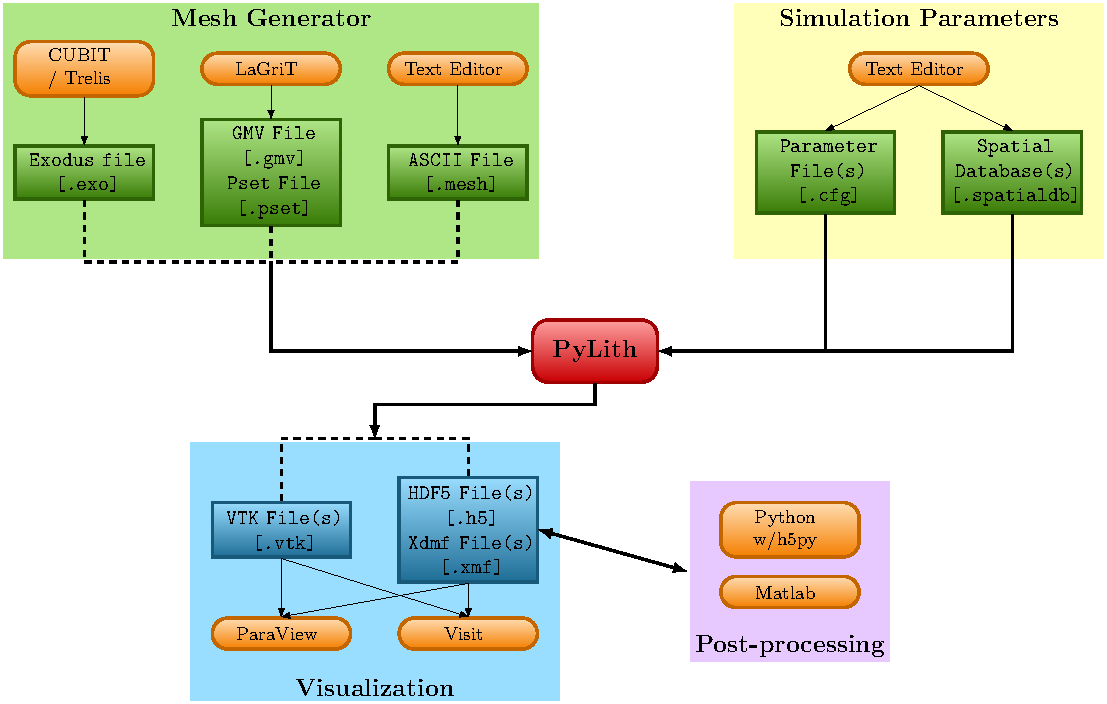
\includegraphics[width=5in]{runpylith/figs/runpylith} 
  \caption{PyLith requires a finite-element mesh (three different
    mechanisms for generating a mesh are currently supported),
    simulation parameters, and spatial databases (defining the spatial
    variation of various parameters).  PyLith writes the solution
    output to either VTK or HDF5/Xdmf files, which can be visualized
    with ParaView or Visit. Post-processing is generally done using
    the HDF5 files with Python or Matlab scripts.}
\label{fig:pylith:workflow} 
\end{figure}

% ----------------------------------------------------------------------
\section{Defining the Simulation}

The parameters for PyLith are specified as a hierarchy or tree of
modules. The application assembles the hierarchy of modules from user
input and then calls the \object{main} function in the top-level
module in the same manner as a C or C++ program. The behavior of the
application is determined by the modules included in the hierarchy as
specified by the user. The Pyre framework provides the interface for
defining this hierarchy. Pyre properties correspond to simple settings
in the form of strings, integers, and real numbers. Pyre facilities
correspond to software modules. Facilities may have their own
facilities (branches in the tree) and any number of properties. See
Figure \vref{fig:Pyre:Architecture} for the general concept of Pyre
facilities and properties. The top-level object is the PyLith
application with three facilities: \facility{mesher}, \facility{problem},
and \facility{petsc}. The \facility{mesher} specifies how to import the
mesh, the \facility{problem} specifies the physical properties, boundary
conditions, etc., and \facility{petsc} is used to specify PETSc
settings. Appendix \vref{cha:components} contains a list of the
components provided by PyLith and spatialdata.


\subsection{Setting PyLith Parameters}
\label{sec:setting:parameters}

There are several methods for setting input parameters for the
\filename{pylith} executable: via the command line or by using a text
file in \filename{.cfg} or \filename{.pml} format. Both facilities and
properties have default values provided, so you only need to set
values when you want to deviate from the default behavior.


\subsubsection{Units}

All dimensional parameters require units. The units are specified
using Python and FORTRAN syntax, so square meters is m**2. Whitespace
is not allowed in the string, for units and dimensioned quantities
are multiplied by the units string; for example, two meters per second
is 2.0*m/s. Available units are shown in Table \vref{tab:pyre:units}

\begin{table}[htbp]
\caption{Pyre supported units. Aliases are in parentheses.}
\label{tab:pyre:units}
\begin{tabular}{lp{5in}}
\textbf{Scale} & \textbf{Available Units} \\
\hline 
length & meter (m), micrometer (um, micron), millimeter (mm), centimeter (cm),
kilometer (km), inch, foot, yard, mile \\
time & second (s), nanosecond (ns), microsecond (us), millisecond (ms), minute,
hour, day, year \\
mass & kilogram (kg), gram (g), centigram (cg), milligram (mg), ounce, pound,
ton \\
pressure & pascal (Pa), kPa, MPa, GPa, bar, millibar, atmosphere (atm) \\
\hline 
\end{tabular}
\end{table}


\subsubsection{Using the Command Line}

The \commandline{-}-help} command line argument displays links to useful
resources for learning PyLith.

Pyre uses the following syntax to change properties from the command
line. To change the value of a property of a component, use
\commandline{-{}-COMPONENT.PROPERTY=VALUE}. Each component is attached
to a facility, so the option above can also be written as
\commandline{-{}-FACILITY.PROPERTY=VALUE}.  Each facility has a
default component attached to it. A different component can be
attached to a facility by \commandline{-{}-FACILITY=NEW\_COMPONENT}.

PyLith's command-line arguments can control Pyre and PyLith properties
and facilities, MPI settings, and PETSc settings. All PyLith-related
properties are associated with the \facility{pylithapp} component. You
can get a list of all of these top-level properties along with a
description of what they do by running PyLith with the
\commandline{-{}-help-properties} command-line argument. To get
information on user-configurable facilities and components, you can
run PyLith with the \commandline{-{}-help-components} command-line
argument. To find out about the properties associated with a given
component, you can run PyLith with the
\commandline{-{}-COMPONENT.help-properties} flag:
\begin{shell}
$$ pylith --problem.help-properties
# Show problem components.
$$ pylith --problem.help-components
# Show bc components (bc is a component of problem).
$$ pylith --problem.bc.help-components
# Show bc properties.
$$ pylith --problem.bc.help-properties
\end{shell}


\subsubsection{Using a {\ttfamily .cfg} File}

Entering all those parameters via the command line involves the risk
of typographical errors. You
will generally find it easier to collect parameters into a
\filename{.cfg} file. The file is composed of one or more sections
which are formatted as follows:
\begin{cfg}
<h>[pylithapp.COMPONENT1.COMPONENT2]</h>
# This is a comment.

<f>FACILITY3</f> = COMPONENT3
<p>PROPERTY1</p> = VALUE1
<p>PROPERTY2</p> = VALUE2 ; this is another comment
\end{cfg}

\tip{We strongly recommend that you use \filename{.cfg} files for your
  work.  The files are syntax-highlighted in the vim editor.}


\subsubsection{Using a {\ttfamily.pml} File}

A \filename{.pml} file is an XML file that specifies parameter values
in a highly structured format. It is composed of nested sections which
are formatted as follows:
\begin{lstlisting}[basicstyle=\ttfamily,frame=tb]{language=xml}
<component~name="COMPONENT1">
    <component~name="COMPONENT2">
        <property~name="PROPERTY1">VALUE1</property>
        <property~name="PROPERTY2">VALUE2</property>
    </component>
</component>
\end{lstlisting}
XML files are intended to be read and written by machines, not edited
manually by humans. The \filename{.pml} file format is intended for
applications in which PyLith input files are generated by another
program, e.g., a GUI, web application, or a high-level structured
editor. This file format will not be discussed further here, but if
you are interested in using \filename{.pml} files, note that \filename{.pml}
files and \filename{.cfg} files can be used interchangeably; in the
following discussion, a file with a \filename{.pml} extension can be
substituted anywhere a \filename{.cfg} file can be used.


\subsubsection{Specification and Placement of Configuration Files}

Configuration files may be specified on the command line:
\begin{shell}
$$ pylith example.cfg
\end{shell}
In addition, the Pyre framework searches for configuration files named
\filename{pylithapp.cfg} in several predefined locations. You may put
settings in any or all of these locations, depending on the scope
you want the settings to have:
\begin{enumerate}
\item \filename{\$PREFIX/etc/pylithapp.cfg}, for system-wide settings;
\item \filename{\$HOME/.pyre/pylithapp/pylithapp.cfg}, for user
  settings and preferences;
\item the current directory (\filename{./pylithapp.cfg}), for local
  overrides.
\end{enumerate}

\important{The Pyre framework will search these directories for
  \filename{.cfg} files matching the names of components (for example,
  \filename{timedependent.cfg}, \filename{faultcohesivekin.cfg},
  \filename{greensfns.cfg}, \filename{pointforce.cfg}, etc) and will
  attempt to assign all parameters in those files to the respective
  component.}

\important{Parameters given directly on the command line will override
  any input contained in a configuration file. Configuration files
  given on the command line override all others. The
  \filename{pylithapp.cfg} files placed in (3) will override those in
  (2), (2) overrides (1), and (1) overrides only the built-in
  defaults.}

All of the example problems are set up using configuration files and specific problems are defined by including
the appropriate configuration file on the command-line. Referring
to the directory \filename{examples/twocells/twohex8}, we have the
following.
\begin{shell}
$$ ls -1 *.cfg
axialdisp.cfg
dislocation.cfg
pylithapp.cfg
sheardisp.cfg
\end{shell}
The settings in \filename{pylithapp.cfg} will be read automatically, and additional
settings are included by specifying one of the other files on the
command-line:
\begin{shell}
$$ pylith axialdisp.cfg
\end{shell}
If you want to see what settings are being used, you can either examine
the \filename{.cfg} files, or use the help flags as described above:
\begin{shell}
# Show components for the 'problem' facility.
$$ pylith axialdisp.cfg --problem.help-components
# Show properties for the 'problem' facility.
$$ pylith axialdisp.cfg --problem.help-properties
# Show components for the 'bc' facility.
$$ pylith axialdisp.cfg --problem.bc.help-components
# Show properties for the 'bc' facility.
$$ pylith axialdisp.cfg --problem.bc.help-properties
\end{shell}
This is generally a more useful way of determining problem settings,
since it includes default values as well as those that have been specified
in the \filename{.cfg} file.


\subsubsection{List of PyLith Parameters ({\ttfamily pylithinfo})}
\label{sec:pylithinfo}

The Python application \filename{pylithinfo} writes all of the current
parameters to a text file or JSON file (default). The default name of the JSON is \filename{pylith\_parameters.json}.
The usage synopsis is
\begin{shell}
$$ pylithinfo [--verbose-false] [--format={ascii,json} [--filename=pylith_parameters.json] PYLITH_ARGS
\end{shell}
where \commandline{-{}-verbose-false} turns off printing the descriptions of
the properties and components as well as the location where the
current value was set, \commandline{-{}-format=ascii} changes the
output format to a simple ASCII file, and
\commandline{-{}-filename=pylith\_parameters.json} sets the name of the
output file. The PyLith Parameter Viewer (see Section
\ref{sec:pylith:parameter:viewer}) provides a graphic user interface
for examining the JSON parameter file. 


\subsection{Mesh Information (\ttfamily{mesher})}

Geometrical and topological information for the finite element mesh
may be provided by exporting an Exodus II format file from
CUBIT/Trelis, by exporting a GMV file and an accompanying Pset file
from LaGriT, or by specifying the information in PyLith mesh ASCII
format. See Chapter \vref{cha:examples} for examples.

PyLith supports linear cells in 2D (Figure \vref{fig:2D:cells}), and
3D (Figure \vref{fig:3D:cells}).  The vertex ordering must follow the
convention shown in Figures \vref{fig:2D:cells}-\vref{fig:3D:cells}.
PyLith no longer supports use of quadratic cells using the PyLith
ASCII mesh format. In the next release, we plan to support higher
order discretizations via PETSc finite-element features from meshes
with linear cells as input.

The mesh information defines the vertex coordinates and specifies
the vertices composing each cell in the mesh. The mesh information
must also define at least one set of vertices for which displacement
(Dirichlet) boundary conditions will be provided. In most realistic
problems, there will be several vertex groups, each with a unique
identifying label. For example, one group might define a surface of
the mesh where displacement (Dirichlet) boundary conditions will be
applied, another might define a surface where traction (Neumann) boundary
conditions will be applied, while a third might specify a surface
that defines a fault. Similarly, the mesh information contains cell
labels that define the material type for each cell in the mesh. For
a mesh with a single material type, there will only be a single label
for every cell in the mesh. See Chapters \vref{cha:material:models}
and \vref{cha:boundary:interface:conditions} for more detailed discussions
of setting the materials and boundary conditions.

\begin{figure}[htbp]
  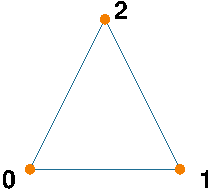
\includegraphics{runpylith/figs/tri3}\hspace*{0.5in}%
  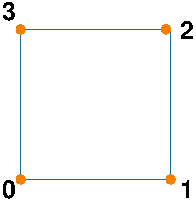
\includegraphics{runpylith/figs/quad4}
  \caption{Linear cells available for 2D problems are the triangle
    (left) and the quadrilateral (right).}
  \label{fig:2D:cells}
\end{figure}

\begin{figure}[htbp]
  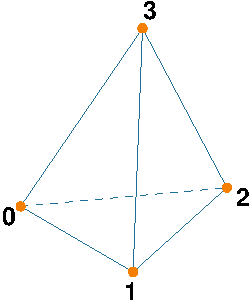
\includegraphics{runpylith/figs/tet4}\hspace*{0.5in}%
  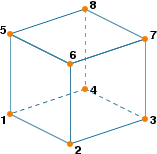
\includegraphics{runpylith/figs/hex8}
  \caption{Linear cells available for 3D problems are the tetrahedron (left)
    and the hexahedron (right).}
  \label{fig:3D:cells}
\end{figure}

\subsubsection{\object{Mesh Importer}}

The default mesher component is \object{MeshImporter}, which provides
the capabilities of reading the mesh from files. The \object{MeshImporter} has
several properties and facilities:
\begin{inventory}
  \propertyitem{reorder\_mesh}{Reorder the vertices and cells using the
    reverse Cuthill-McKee algorithm (default is False)}
  \facilityitem{reader}{Reader for a given type of mesh (default is
    \object{MeshIOAscii}).}
  \facilityitem{distributor}{Handles
    distribution of the mesh among processors.}
  \facilityitem{refiner}{Perform global uniform mesh refinement after
    distribution among processors (default is no refinement).}
\end{inventory}
Reordering the mesh so that vertices and cells connected topologically
also reside close together in memory improves overall performance
and can improve solver performance as well.

\warning{The coordinate system associated with the mesh must be a
  Cartesian coordinate system, such as a generic Cartesian coordinate
  system or a geographic projection.}

\subsubsection{\object{MeshIOAscii}}

The \object{MeshIOAscii} object is intended for reading small, simple
ASCII files containing a mesh constructed by hand. We use this file
format extensively in the examples. Appendix \vref{sec:format:MeshIOAscii}
describes the format of the files. The properties and facilities of
the \object{MeshIOAscii} object include:
\begin{inventory}
\propertyitem{filename}{Name of the mesh file.}
\facilityitem{coordsys}{Coordinate system associated with the mesh.}
\end{inventory}

\subsubsection{\object{MeshIOCubit}}
\label{sec:MeshIOCubit}

The \object{MeshIOCubit} object reads the NetCDF Exodus II files output from
CUBIT/Trelis. Beginning with CUBIT 11.0, the names of the nodesets are included
in the Exodus II files and PyLith can use these nodeset names or revert
to using the nodeset ids. The properties and facilities associated
with the \object{MeshIOCubit} object are:
\begin{inventory}
\propertyitem{filename}{Name of the Exodus II file.}
\propertyitem{use\_nodeset\_names}{Identify nodesets by name rather than id
(default is True).}
\facilityitem{coordsys}{Coordinate system associated with the mesh.}
\end{inventory}

\subsubsection{\object{MeshIOLagrit}}
\label{sec:MeshIOLagrit}

The \object{MeshIOLagrit} object is used to read ASCII and binary GMV and PSET
files output from LaGriT. PyLith will automatically detect whether
the files are ASCII or binary. We attempt to provide support for experimental
64-bit versions of LaGriT via flags indicating whether the FORTRAN
code is using 32-bit or 64-bit integers. The \object{MeshIOLagrit} properties
and facilities are:
\begin{inventory}
  \propertyitem{filename\_gmv}{Name of GMV file.}
  \propertyitem{filename\_pset}{Name of the PSET file.}
  \propertyitem{flip\_endian}{Flip the endian of values when reading
    binary files (default is False).}
  \propertyitem{io\_int32}{Flag
    indicating that PSET files use 32-bit integers (default is True).}
  \propertyitem{record\_header\_32bt}{Flag indicating FORTRAN record header is
    32-bit (default is True).}
\facilityitem{coordsys}{Coordinate system associated with mesh.}
\end{inventory}

\warning{The PyLith developers have not used LaGriT since around 2008
  and the most recent release appears to have been in 2010.}

\subsubsection{\object{Distributor}}

The distributor uses a partitioner to compute which cells should be
placed on each processor, computes the overlap among the processors,
and then distributes the mesh among the processors. The type of
partitioner is set via PETSc settings. The properties and facilities
of the \object{Distributor} include:
\begin{inventory}
\propertyitem{partitioner}{Name of mesh partitioner ['chaco','parmetis'].}
\propertyitem{write\_partition}{Flag indicating that the partition information
should be written to a file (default is False).}
\facilityitem{data\_writer}{Writer for partition information (default
  is \object{DataWriterVTK} for VTK output).}
\end{inventory}
An example of setting the partitioner in a \filename{pylithapp.cfg}
  file is:
\begin{cfg}
<h>[pylithapp.mesh_generator.distributor]</h>
<p>partitioner</p> = chaco ; Options are 'chaco' (default) and 'parmetis'.
\end{cfg}
METIS/ParMETIS are not included in the PyLith binaries due to licensing
issues. 


\subsubsection{\object{Refiner}}

The refiner is used to decrease node spacing by a power of two by
recursively subdividing each cell by a factor of two. In a 2D triangular
mesh a node is inserted at the midpoint of each edge, splitting each
cell into four cells (see Figure \vref{fig:uniform:refinement:2x}).
In a 2D quadrilateral mesh a node is inserted at the midpoint of each
edge and at the centroid of the cell, splitting each cell into four
cells. In a 3D tetrahedral mesh a node is inserted at the midpoint
of each edge, splitting each cell into eight cells. In a 3D hexahedral
mesh a node is inserted at the midpoint of each edge, the centroid
of each face, and at the centroid of the cell, splitting each cell
into eight cells.

\begin{figure}[htbp]
  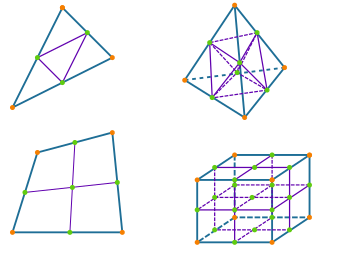
\includegraphics[scale=1.25]{runpylith/figs/refinement2x}
  \caption{Global uniform mesh refinement of 2D and 3D linear
    cells. The blue lines and orange circles identify the edges and
    vertices in the original cells. The purple lines and green circles
    identify the new edges and vertices added to the original cells to
    refine the mesh by a factor of two.}
\label{fig:uniform:refinement:2x}
\end{figure}

Refinement occurs after distribution of the mesh among processors.
This allows one to run much larger simulations by (1) permitting the
mesh generator to construct a mesh with a node spacing largeer than
that needed in the simulation and (2) operations performed in serial
during the simulation setup phase, such as, adjusting the topology
to insert cohesive cells and distribution of the mesh among processors
uses this much smaller coarse mesh. For 2D problems the global mesh
refinement increases the maximum problem size by a factor of $4^{n}$,
and for 3D problems it increases the maximum problem size by a factor
of $8^{n}$, where $n$ is the number of recursive refinement levels.
For a tetrahedral mesh, the element quality decreases with refinement
so $n$ should be limited to 1-2.


\subsection{Problem Specification (\facility{problem})}

The problem component specifies the basic parameters of the simulation,
including the physical properties, the boundary conditions, and interface
conditions (faults). The current release of PyLith contains two types
of problems, \object{TimeDependent} for use in static, quasi-static,
and dynamic simulations and \object{GreensFns} for computing static
Green's functions. The general properties facilities include:
\begin{inventory}
  \propertyitem{dimension}{Spatial dimension of problem space.}
  \facilityitem{normalizer}{Scales used to nondimensionalize the
    problem (default is \object{NondimElasticQuasistatic}).}
  \facilityitem{materials}{Array of materials comprising the domain
    (default is [material]).}
  \facilityitem{bc}{Array of boundary conditions (default is none).}
  \facilityitem{interfaces}{Array of interface conditions, i.e., faults
    (default is none).}
  \facilityitem{gravity\_field}{Gravity field used to construct body
    forces (default is none).}
  \facilityitem{progress\_ monitor}{Show progress of running
    simulation.}
\end{inventory}
An example of setting these parameters in a \filename{.cfg} file for
a problem is:
\begin{cfg}
<h>[pylithapp.timedependent]</h>
<p>dimension</p> = 3
<f>normalizer</f> = spatialdata.units.NondimElasticQuasistatic
<f>materials</f> = [elastic, viscoelastic]
<f>bc</f> = [boundary_east, boundary_bottom, boundary_west]
<f>interfaces</f> = [SanAndreas, SanJacinto]
<f>gravity_field</f> = spatialdata.spatialdb.GravityField
\end{cfg}

\subsubsection{Nondimensionalization (\facility{normalizer})}

PyLith nondimensionalizes all parameters provided by the user so that
the simulation solves the equations using nondimensional quantities.
This permits application of PyLith to problems across a vast range
of spatial and temporal scales. The scales used to nondimensionalize
the problem are length, pressure, density, and time. PyLith provides
two normalizer objects to make it easy to provide reasonable scales
for the nondimensionalization. The \object{NondimElasticQuasistatic}
normalizer (which is the default) has the following properties:
\begin{inventory}
  \propertyitem{length\_scale}{Distance to nondimensionalize length
    (default is 1.0 km).}
  \propertyitem{shear\_modulus}{Shear modulus to nondimensionalize
    pressure (default is 3.0e+10 Pa).}
  \propertyitem{relaxation\_time}{Relaxation time to
    nondimensionalize time (default is 1.0 year).}
\end{inventory}
An example of setting these parameters in a \filename{.cfg} file for
a problem is:
\begin{cfg}
<h>[pylithapp.timedependent.normalizer]</h>
<p>length_scale</p> = 1.0*km
<p>shear_modulus</p> = 3.0e+10*Pa
<p>relaxation_time</p> = 1.0*yr
\end{cfg}
The \object{NondimElasticDynamic} normalizer has the following
properties:
\begin{inventory}
  \propertyitem{shear\_wave\_speed}{Shear wave speed used to
    nondimensionalize length and pressure (default is 3.0 km/s).}
  \propertyitem{mass\_density}{Mass density to nondimensionalize
    density and pressure (default is 3.0e+3 kg/m$^{3}$).}
  \propertyitem{wave\_period}{Period of seismic waves used to
    nondimensionalize time (default is 1.0 s).}
\end{inventory}
An example of setting these parameters in a \filename{.cfg} file for
a problem is:
\begin{cfg}
<h>[pylithapp.timedependent.normalizer]</h>
<p>shear_wave_speed</p> = 3.0*km/s
<p>mass_density</p> = 3.0e+3*kg/m**3
<p>wave_period</p> = 1.0*s
\end{cfg}

\important{The default nondimensionalization is reasonable for many
  problems; however, it may be necessary to change the default values
  in some cases. When doing this, keep in mind that the
  nondimensionalization generally applies to the minimum values
  encountered for a problem.  For example, in a quasistatic problem,
  the \property{length\_scale} should be on the order of the minimum
  cell size. Similarly, the \property{relaxation\_time} should be on
  the order of the minimum relaxation time.}

\subsection{Finite-Element Integration Settings}

PyLith uses numerical quadrature to evaluate the finite-element
integrals for the residual and system Jacobian (see Chapter
\vref{cha:governing:equations}).  PyLith employs FIAT (finite element
automatic tabulator) to compute the basis functions and their
derivatives at the quadrature points for various quadrature schemes
and cell shapes. The parameters for Lagrange cells (lines,
quadrilaterals, hexahedra) are specified using the
\object{FIATLagrange} object, whereas the parameters for Simplex cells
(lines, triangles, tetrahedra) are specified using the
\object{FIATSimplex}x object. Both objects use the same set of
parameters and PyLith will setup the basis functions and quadrature
scheme appropriately for the two families of cells. The quadrature
scheme and basis functions must be set for each material and boundary
condition involving finite-element integrations (Dirichlet boundary
conditions are constraints and do not involve
integrations). Furthermore, the integration schemes can be set
independently. The current version of PyLith supports basis functions
with linear variations in the field (P1); support for higher order
cells will be added in the future. The properties for the
\object{FIATLagrange} and \object{FIATSimplex} objects are
\begin{inventory}
  \propertyitem{dimension}{Dimension of the cell (0,1,2,3; default is
    3).}
  \propertyitem{degree}{Degree of the finite-element cell (default is
    1).}
  \propertyitem{order}{Order of quadrature rule (default is degree+1);
    hardwired to be equal to degree for faults.}
  \propertyitem{collocate\_quad}{Collocate quadrature points with
    vertices (default is False); hardwired to True for faults.}
\end{inventory}
See Section \vref{sec:material:parameters} for an example of setting
these properties for a material.


\subsection{PETSc Settings (\facility{petsc})}
\label{sec:petsc:options}

In quasti-static problems with implicit time-stepping, PyLith relies
on PETSc for the linear algebra computations, including linear Krylov
subspace solvers and nonlinear solvers. For dynamic problems, lumping
the mass matrix and using explicit time-stepping is much more efficient;
this permits solving the linear system with a trivial solver so we
do not use a PETSc solver in this case (see Section \vref{sec:solvers}).

PETSc options can be set in \filename{.cfg} files in sections
beginning with \texttt{[pylithapp.petsc]}. The options of primary
interest in the case of PyLith are shown in Table
\vref{tab:petsc:options:defaults}.  PETSc options are used to control
the selection and settings for the solvers underlying the SolverLinear
and SolverNonlinear objects discussed in Section \vref{sec:solvers}. A
very wide range of elasticity problems in quasi-static simulations can
be solved with reasonable runtimes by replacing the default Jacobi
preconditioner with the Additive Schwarz Method (ASM) using Incomplete
LU (ILU) factorization by default (see Table
\vref{tab:petsc:options:recommended}). A more advanced set of solver
settings that may provide better performance in many elasticity
problems are given in Table \vref{tab:petsc:options:advanced}. These
are available in
\filename{\$PYLITH\_DIR/share/settings/solver\_fault\_fieldsplit.cfg.}
These settings are limited to problems where we store the stiffness
matrix as a nonsymmetric sparse matrix and require additional settings
for the formulation,
\begin{cfg}
<h>[pylithapp.timedependent.formulation]</h>
<p>split_fields</p> = True
<p>use_custom_constraint_pc</p> = True ; Use only if problem contains a fault
<p>matrix_type</p> = aij
\end{cfg}

\important{These settings are only available if you build PETSc with
  the ML package. These features are included in the PyLith binary
  packages.}

\warning{The split fields and algebraic multigrid preconditioning
  currently fails in problems with a nonzero null space. This most
  often occurs when a problem contains multiple faults that extend
  through the entire domain and create subdomains without any
  Dirichlet boundary conditions. The current workaround is to use the
  Additive Schwarz preconditioner without split fields.  See Section
  \vref{sec:Troubleshooting} for the error message encountered in this
  situation.}

These more advanced settings allow the displacement fields and Lagrange
multipliers for fault tractions to be preconditioned separately. This
usually results in a much stronger preconditioner. In simulations
with fault slip, the degrees of freedom associated with the Lagrange
multipliers should be preconditioned with a custom preconditioner
that uses a diagonal approximation of the Schur complement.

\begin{table}[htbp]
  \caption{\label{tab:petsc:options:defaults}Useful command-line arguments for
    setting PETSc options.}
  \begin{tabular}{lcp{4.5in}}
    \textbf{Property} & \textbf{Default Value} & \textbf{Description} \\
    \hline 
    \property{log\_view} & \textit{false} & Print logging objects and events. \\
    \property{ksp\_monitor} & \textit{false} & Dump preconditioned residual norm to stdout. \\
    \property{ksp\_view} & \textit{false} & Print linear solver parameters. \\
    \property{ksp\_rtol} & \textit{1.0e-05} & Convergence tolerance for relative decrease in residual norm. \\
    \property{snes\_monitor} & \textit{false} & Dump residual norm to stdout for each nonlinear solve iteration. \\
    \property{snes\_view} & \textit{false} & Print nonlinear solver parameters. \\
    \property{snes\_rtol} & \textit{1.0e-5} & Convergence tolerance for relative decrease in residual norm. \\
    \property{pc\_type} & \textit{jacobi} & Set preconditioner type. See \href{http://www.mcs.anl.gov/petsc/petsc-as/documentation/linearsolvertable.html}{PETSc documentation}
                                            for a list of all preconditioner types. \\
    \property{ksp\_type} & \textit{gmres} & Set linear solver type. See \href{http://www.mcs.anl.gov/petsc/petsc-as/documentation/linearsolvertable.html}{PETSc documentation}
                                            for a list of all solver types. \\
    \hline 
  \end{tabular}
\end{table}

\begin{table}[htbp]
  \caption{PETSc options that provide moderate
    performance in a wide range of quasi-static elasticity problems.}
  \label{tab:petsc:options:recommended}
  \begin{tabular}{lcp{3.5in}}
    \textbf{Property} & \textbf{Value} & \textbf{Description} \\
\hline 
    \property{pc\_type} & \textit{asm} & Additive Schwarz method. \\
    \property{ksp\_type} & \textit{gmres} & GMRES method from Saad and Schultz. \\
    \property{sub\_pc\_factor\_shift\_type} & \emph{nonzero} & Turn on nonzero shifting for factorization. \\
    \property{ksp\_max\_it} & \emph{100} & Maximum number of iterations permitted in linear solve. Depends on problem size. \\
    \property{ksp\_gmres\_restart} & \textit{50} & Number of iterations after which Gram-Schmidt orthogonalization is restarted. \\
    \property{ksp\_rtol} & \textit{1.0e-08} & Linear solve convergence tolerance for relative decrease in residual norm. \\
    \property{ksp\_atol} & \textit{\emph{1.0e-12}} & Linear solve convergence tolerance for absolute value of residual norm. \\
    \property{ksp\_converged\_reason} & \textit{true} & Indicate why iterating stopped in linear solve. \\
    \property{snes\_max\_it} & \textit{100} & Maximum number of iterations permitted in nonlinear solve. Depends on how nonlinear the problem is. \\
    \property{snes\_rtol} & \textit{1.0e-08} & Nonlinear solve convergence tolerance for relative decrease in residual norm. \\
    \property{snes\_atol} & \textit{1.0e-12} & Nonlinear solve convergence tolerance for absolute value of residual norm. \\
    \property{snes\_converged\_reason} & \textit{true} & Indicate why iterating stopped in nonlinear solve. \\
\hline 
\end{tabular}
\end{table}

\begin{table}[htbp]
  \caption{PETSc options used with split fields
    algebraic multigrid preconditioning that often provide improved performance
    in quasi-static elasticity problems with faults.}
  \label{tab:petsc:options:advanced}
  \begin{tabular}{lcp{2.5in}}
    \textbf{Property} & \textbf{Value} & \textbf{Description} \\
    \hline 
    \property{\footnotesize{fs\_pc\_type}} & \textit{field\_split} & Precondition fields separately.\\
    \property{\footnotesize{fs\_pc\_use\_amat}} & \textit{true} & Use diagonal blocks from the true operator, rather than the preconditioner.\\
    \property{\footnotesize{fs\_pc\_fieldsplit\_type}} & \textit{multiplicative} & Apply each field preconditioning in sequence, which is stronger than all-at-once (additive).\\
    \property{\footnotesize{fs\_fieldsplit\_displacement\_pc\_type}} & \textit{ml} & Multilevel algebraic multigrid preconditioning using Trilinos/ML via PETSc.\\
    \property{\footnotesize{fs\_fieldsplit\_lagrange\_multiplier\_pc\_type}} & \textit{jacobi} & Jacobi preconditioning for Lagrange multiplier block\\
    \property{\footnotesize{fs\_fieldsplit\_displacement\_ksp\_type}} & \textit{preonly} & Apply only the preconditioner.\\
    \property{\footnotesize{fs\_fieldsplit\_lagrange\_multiplier\_ksp\_type}} & \textit{preonly} & Apply only the preconditioner.\\
    \hline 
  \end{tabular}
\end{table}


\subsubsection{Model Verification with PETSc Direct Solvers}

It is often useful to apply a direct solver so that solver convergence
is decoupled from model verification for the purposes of testing.
Unfortunately, the traditional LU factorization solvers cannot be
directly applied in PyLith due to the saddle-point formulation used
to accomodate the fault slip constraints. However, we can combine
an LU factorization of the displacement sub-block with a full Schur
complement factorization using the PETSc FieldSplit preconditioner.
If the solver for the Schur complement S is given a very low tolerance,
this is effectively a direct solver. The options given below will
construct this solver in PyLith. These settings are available in \filename{\$PYLITH\_DIR/share/settings/solver\_fault\_exact.cfg}.
\begin{cfg}
<h>[pylithapp.timedependent.formulation]</h>
<p>split_fields</p> = True
<p>matrix_type</p> = aij

<h>[pylithapp.petsc]</h>
<p>fs_pc_type</p> = fieldsplit
<p>fs_pc_use_amat</p> = True
<p>fs_pc_fieldsplit_type</p> = schur
<p>fs_pc_fieldsplit_schur_factorization_type</p> = full
<p>fs_fieldsplit_displacement_ksp_type</p> = preonly
<p>fs_fieldsplit_displacement_pc_type</p> = lu
<p>fs_fieldsplit_lagrange_multiplier_pc_type</p> = jacobi
<p>fs_fieldsplit_lagrange_multiplier_ksp_type</p> = gmres
<p>fs_fieldsplit_lagrange_multiplier_ksp_rtol</p> = 1.0e-11
\end{cfg}

% End of file

\section{Time-Dependent Problem (\facilityshape{formulation})}

This type of problem applies to transient static, quasi-static, and
dynamic simulations. The time-dependent problem adds the
\facility{formulation} facility to the general-problem. The
formulation specifies the time-stepping formulation to integrate the
elasticity equation. PyLith provides several alternative formulations,
each specific to a different type of problem.
\begin{description}
\item[\object{Implicit}] Implicit time stepping for static and
   quasi-static problems with infinitesimal strains. The implicit
   formulation neglects inertial terms (see Section
   \vref{eq:elasticity:integral:quasistatic}).
\item[\object{ImplicitLgDeform}] Implicit time stepping for static
  and quasi-static problems including the effects of rigid body motion
  and small strains.  This formulation requires the use of the
  nonlinear solver, which is selected automatically.
\item[\object{Explicit}] Explicit time stepping for dynamic problems
  with infinitesimal strains and lumped system Jacobian. The cell
  matrices are lumped before assembly, permitting use of a vector for
  the diagonal system Jacobian matrix. The built-in lumped solver is
  selected automatically.
\item[\object{ExplicitLgDeform}] Explicit time stepping for dynamic
  problems including the effects of rigid body motion and small
  strains. The cell matrices are lumped before assembly, permitting
  use of a vector for the diagonal system Jacobian matrix. The
  built-in lumped solver is selected automatically.
\item[\object{ExplicitTri3}] Optimized elasticity formulation for
  linear triangular cells with one point quadrature for dynamic
  problems with infinitesimal strains and lumped system Jacobian. The
  built-in lumped solver is selected automatically.
\item[\object{ExplicitTet4}] Optimized elasticity formulation for
  linear tetrahedral cells with one point quadrature for dynamic
  problems with infinitesimal strains and lumped system Jacobian. The
  built-in lumped solver is selected automatically.
\end{description}
In many quasi-static simulations it is convenient to compute a static
problem with elastic deformation prior to computing a transient response.
Up through PyLith version 1.6 this was hardwired into the Implicit
Forumulation as advancing from time step $t=-\Delta t$ to $t=0$,
and it could not be turned off. PyLith now includes a property, \property{elastic\_prestep}
in the TimeDependent component to turn on/off this behavior (the default
is to retain the previous behavior of computing the elastic deformation).

\warning{Turning off the elastic
prestep calculation means the model only deforms when an {\it increment}
in loading or deformation is applied, because the time-stepping formulation
is implemented using the increment in displacement.}

The \object{TimeDependent} properties and facilities include
\begin{inventory}
  \propertyitem{elastic\_preset}{If true, perform a static calculation with elastic
    behavior before time stepping (default is True).}
  \facilityitem{formulation}{Formulation for solving the partial differential
    equation.}
\end{inventory}

\begin{cfg}[\object{TimeDependent} parameters in a \filename{cfg} file]
<h>[pylithapp.timedependent]</h>
<f>formulation</f> = pylith.problems.Implicit ; default
<f>progres_monitor</f> = pylith.problems.ProgressMonitorTime ; default
<p>elastic_preset</p> = True ; default
\end{cfg}
The formulation value can be set to the other formulations in a similar
fashion. 


\subsection{Time-Stepping Formulation}

The explicit and implicit time stepping formulations use a common
set of facilities and properties. The properties and facilities include
\begin{inventory}
\propertyitem{matrix\_type}{Type of PETSc matrix for the system Jacobian (sparse
matrix, default is symmetric, block matrix with a block size of 1).}
\propertyitem{view\_jacobian}{Flag to indicate if system Jacobian (sparse matrix)
should be written to a file (default is false).}
\propertyitem{split\_fields}{Split solution field into a displacement portion
(fields 0..ndim-1) and a Lagrange multiplier portion (field ndim)
to permit application of sophisticated PETSc preconditioners (default
is false).}
\facilityitem{time\_step}{Time step size specification (default is \object{TimeStepUniform} (uniform time step).}
\facilityitem{solver}{Type of solver to use (default is \object{SolverLinear}).}
\facilityitem{output}{Array of output managers for output of the solution (default
is [output]).}
\facilityitem{jacobian\_viewer}{Viewer to dump the system Jacobian (sparse matrix)
to a file for analysis (default is PETSc binary).}
\end{inventory}

\begin{cfg}[Time-stepping formulation parameters in a \filename{cfg} file]
<h>[pylithapp.timedependent.formulation]</h>
<p>matrix_type</p> = sbaij ; Non-symmetric sparse matrix is 'aij'
<p>view_jacobian</p> = false

# Nonlinear solver is pylith.problems.SolverNonlinear
<f>solver</f> = pylith.problems.SolverLinear
<f>output</f> = [domain, ground_surface]
<f>time_step</f> = pylith.problems.TimeStepUniform
\end{cfg}

\subsection{Numerical Damping in Explicit Time Stepping}

In explicit time-stepping formulations for elasticity, boundary conditions
and fault slip can excite short waveform elastic waves that are not
accurately resolved by the discretization. We use numerical damping
via an artificial viscosity\cite{Knopoff:Ni:2001,Day:Ely:2002} to
reduce these high frequency oscillations. In computing the strains
for the elasticity term in equation \vref{eq:elasticity:integral:dynamic:t},
we use an adjusted displacement rather than the actual displacement,
where 
\begin{equation}
\vec{u}^{adj}(t)=\vec{u}(t)+\eta^{*}\Delta t\vec{\dot{u}}(t),
\end{equation}
$\vec{u}^{adj}(t)$ is the adjusted displacement at time t, $\vec{u}(t)$is
the original displacement at time (t), $\eta^{*}$is the normalized
artificial viscosity, $\Delta t$ is the time step, and $\vec{\dot{u}}(t)$
is the velocity at time $t$. The default value for the normalized
artificial viscosity is 0.1. We have found values in the range 0.1-0.4
sufficiently suppress numerical noise while not excessively reducing
the peak velocity. An example of setting the normalized artificial
viscosity in a \filename{cfg} file is
\begin{cfg}
<h>[pylithapp.timedependent.formulation]</h>
<p>norm_viscosity</p> = 0.2
\end{cfg}

\subsection{Solvers}
\label{sec:solvers}

PyLith supports three types of solvers. The linear solver,
SolverLinear, corresponds to the PETSc KSP solver and is used in
linear problems with linear elastic and viscoelastic bulk constitutive
models and kinematic fault ruptures. The nonlinear solver,
SolverNonlinear, corresponds to the PETSc SNES solver and is used in
nonlinear problems with nonlinear viscoelastic or elastoplastic bulk
constitutive models, dynamic fault ruptures, or problems involving
finite strain (small strain formulation).  The lumped solver
(SolverLumped) is a specialized solver used with the lumped system
Jacobian matrix. The options for the PETSc KSP and SNES solvers are
set via the top-level PETSc options (see Section
\vref{sec:petsc:options} and the PETSc documentation
\url{www.mcs.anl.gov/petsc/petsc-as/documentation/index.html}).


\subsection{Time Stepping}
\label{sec:time-stepping}

PyLith provides three choices for controlling the time step in time-dependent
simulations. These include (1) a uniform, user-specified time step
(which is the default), (2) user-specified time steps (potentially
nonuniform), and (3) automatically calculated (potentially nonuniform)
time steps. The procedure for automatically selecting time steps requires
that the material models provide a reasonable estimate of the time
step for stable time integration. In general, quasi-static simulations
with viscoelastic materials should use automatically calculated time
steps and dynamic simulations should use a uniform, user-specified
time step. Note that all three of the time stepping schemes make use
of the computed stable time step (see \vref{sec:stable:time:step}).
When using user-specified time steps, the value is checked against
the computed stable time step. The automatically calculated time step
comes from the computed stable time step.

\warning{Varying the time step within a simulation requires
  recomputing the Jacobian of the system whenever the time step
  changes, which can greatly increase the runtime if the time-step
  size changes frequently.}

\subsubsection{Uniform, User-Specified Time Step (\object{TimeStepUniform})}

With a uniform, user-specified time step, the user selects the time
step that is used over the entire duration of the simulation. If this
value exceeds the computed stable time step at any time, PyLith will
terminate with an error. The properties for the uniform, user-specified
time step are:
\begin{inventory}
\propertyitem{total\_time}{Time duration for simulation (default is 0.0 s).}
\propertyitem{start\_time}{Start time for simulation (default is 0.0 s).}
\propertyitem{dt}{Time step for simulation.}
\end{inventory}

\begin{cfg}[\object{TimeStepUniform} parameters in a \filename{cfg} file]
<h>[pylithapp.problem.formulation]</h>
<p>time_step</p> = pylith.problems.TimeStepUniform ; Default value

<h>[pylithapp.problem.formulation.time_step]</h>
<p>total_time</p> = 1000.0*year
<p>dt</p> = 0.5*year
\end{cfg}

\subsubsection{Nonuniform, User-Specified Time Step (\object{TimeStepUser})}

The nonuniform, user-specified, time-step implementation allows the
user to specify the time steps in an ASCII file (see Section
\vref{sec:format:TimeStepUser} for the format specification of the
time-step file). If the total duration exceeds the time associated
with the time steps, then a flag determines whether to cycle through
the time steps or to use the last specified time step for the time
remaining. Similar to the uniform time step, if the user-specified
time step size exceeds the computed stable time step at any time,
PyLith will terminate with an error.  The properties for the
nonuniform, user-specified time step are:
\begin{inventory}
\propertyitem{total\_time}{Time duration for simulation.}
\propertyitem{filename}{Name of file with time-step sizes.}
\propertyitem{loop\_steps}{If true, cycle through time steps, otherwise keep
using last time-step size for any time remaining.}
\end{inventory}

\begin{cfg}[\object{TimeStepUser} parameters in a \filename{cfg} file]
<h>[pylithapp.problem.formulation]</h>
<f>time_step</f> = pylith.problems.TimeStepUser ; Change the time step algorithm

<h>[pylithapp.problem.formulation.time_step]</h>
<p>total_time</p> = 1000.0*year
<p>filename</p> = timesteps.txt
<p>loop_steps</p> = false ; Default value
\end{cfg}

\subsubsection{Nonuniform, Automatic Time Step (\object{TimeStepAdapt})}

This time-step implementation automatically calculates a time step
size based on the constitutive model and rate of deformation. As a
result, this choice for choosing the time step relies on accurate
calculation of a stable time step within each finite-element cell
by the constitutive models. To provide some control over the time-step
selection, the user can control the frequency with which a new time
step is calculated, the time step to use relative to the value determined
by the constitutive models, and a maximum value for the time step.
Note that the stability factor allows the computed time step size
to exceed the computed stable time step. A stability factor of 1.0
would provide a time step size equal to the stable time step, while
a value of 2.0 (default value) would provide a time step size equal
to 1/2 the stable time step. Caution should be used when adjusting
the stability factor to values less than 1.0, as the large time step
size may result in inaccurate solutions. The properties for controlling
the automatic time-step selection are:
\begin{inventory}
\propertyitem{total\_time}{Time duration for simulation.}
\propertyitem{max\_dt}{Maximum time step permitted.}
\propertyitem{adapt\_skip}{Number of time steps to skip between calculating
new stable time step.}
\propertyitem{stability\_factor}{Safety factor for stable time step (default
is 2.0).}
\end{inventory}

\begin{cfg}[\object{TimeStepAdapt} parameters in a \filename{cfg} file]
<h>[pylithapp.problem.formulation]</h>
<p>time_step</p> = pylith.problems.TimeStepAdapt ; Change the time step algorithm

<h>[pylithapp.problem.formulation.time_step]</h>
<p>total_time</p> = 1000.0*year
<p>max_dt</p> = 10.0*year
<p>adapt_skip</p> = 10 ; Default value
<p>stability_factor</p> = 2.0 ; Default value
\end{cfg}

\section{Green's Functions Problem (\object{GreensFns})}

This type of problem applies to computing static Green's functions
for elastic deformation. The \object{GreensFns} problem specializes
the time-dependent facility to the case of static simulations with
slip impulses on a fault. The default formulation is the Implicit
formulation and should not be changed as the other formulations are
not applicable to static Green's functions. In the output files, the
deformation at each ``time step'' is the deformation for a different
slip impulse. The properties provide the ability to select which fault
to use for slip impulses. The only fault component available for use
with the \object{GreensFns} problem is the \object{FaultCohesiveImpulses}
component discussed in Section \vref{sec:fault:cohesive:impulses}.
The \object{GreensFns} properties amd facilities include:
\begin{inventory}
\propertyitem{fault\_id}{Id of fault on which to impose slip impulses.}
\propertyitem{formulation}{Formulation for solving the partial differential
equation.}
\propertyitem{progress\_monitor}{Simple progress monitor via text file.}
\end{inventory}

\begin{cfg}[\object{GreensFns} parameters in a \filename{cfg} file]
<h>[pylithapp]</h>
<f>problem</f> = pylith.problems.GreensFns ; Change problem type from the default

<h>[pylithapp.greensfns]</h>
<p>fault_id</p> = 100 ; Default value
<f>formulation</f> = pylith.problems.Implicit ; default
<f>progres_monitor</f> = pylith.problems.ProgressMonitorTime ; default
\end{cfg}

\warning{The \object{GreensFns} problem generates slip impulses on a
  fault. The current version of PyLith requires that impulses can only
  be applied to a single fault and the fault facility must be set to
  \object{FaultCohesiveImpulses}.}

\section{Progress Monitors}
\newfeature{v2.1.0}

The progress monitors make it easy to monitor the general progress of
long simulations, especially on clusters where stdout is not always
easily accessible. The progress monitors update a simulation's current
progress by writing information to a text file. The information
includes time stamps, percent completed, and an estimate of when the
simulation will finish.

\subsection{\object{ProgressMonitorTime}}

This is the default progress monitor for time-stepping problems. The
monitor calculates the percent completed based on the time at the
current time step and the total simulated time of the simulation,
not the total number of time steps (which may be unknown in simulations
with adaptive time stepping). The \object{ProgressMonitorTime} properties
include:
\begin{inventory}
\propertyitem{update\_percent}{Frequency (in percent) of progress updates.}
\propertyitem{filename}{Name of output file.}
\propertyitem{t\_units}{Units for simulation time in output.}
\end{inventory}

\begin{cfg}[\object{ProgressMonitorTime} parameters in a \filename{cfg} file]
<h>[pylithapp.problem.progressmonitor]</h>
<p>update_percent</p> = 5.0 ; default
<p>filename</p> = progress.txt ; default
<p>t_units</p> = year ; default
\end{cfg}

\subsection{\object{ProgressMonitorStep}}

This is the default progress monitor for problems with a specified
number of steps, such as Green's function problems. The monitor calculates
the percent completed based on the number of steps (e.g., Green's
function impulses completed). The ProgressMonitorStep propertiles
include:
\begin{inventory}
\propertyitem{update\_percent}{Frequency (in percent) of progress updates.}
\propertyitem{filename}{Name of output file.}
\end{inventory}

\begin{cfg}[\object{ProgressMonitorStep} parameters in a \filename{cfg} file]
<h>[pylithapp.problem.progressmonitor]</h>
<p>update_percent</p> = 5.0 ; default
<p>filename</p> = progress.txt ; default
\end{cfg}

% End of file

\section{Databases for Boundaries, Interfaces, and Material Properties}
\label{sec:spatial:databases}

Once the problem has been defined with PyLith parameters, and the
mesh information has been provided, the final step is to specify the
boundary conditions and material properties to be used. The mesh information
provides labels defining sets of vertices to which boundary conditions
or fault conditions will be applied, as well as cell labels that will
be used to define the material type of each cell. For boundary conditions,
the \filename{.cfg} file is used to associate boundary condition types
and spatial databases with each vertex group (see Chapter \vref{cha:boundary:interface:conditions}).
For materials, the \filename{.cfg} file is used to associate material
types and spatial databases with cells identified by the material
identifier (see Figure \vref{fig:material:models}).

The spatial databases define how the boundary conditions or material
property values vary spatially, and they can be arbitrarily complex.
The simplest example for a material database would be a mesh where
all the cells of a given type have uniform properties (``point''
or 0D variation). A slightly more complex case would be a mesh where
the cells of a given type have properties that vary linearly along
a given direction (``line'' or 1D variation). In more complex models,
the material properties might have different values at each point
in the mesh (``volume'' or 3D variation). This might be the case,
for example, if the material properties are provided by a database
of seismic velocities and densities. For boundary conditions the simplest
case would be where all vertices in a given group have the same boundary
condition parameters (``point'' or 0D variation). A more complex
case might specify a variation in the conditions on a given surface
(``area'' or 2D variation). This sort of condition might be used,
for example, to specify the variation of slip on a fault plane. The
examples discussed in Chapter \vref{cha:examples} also contain more
information regarding the specification and use of the spatial database
files.


\subsection{\object{SimpleDB} Spatial Database}

In most cases the default type of spatial database for faults, boundary
conditions, and materials is \object{SimpleDB}. Spatial database files
provide specification of a field over some set of points. There is
no topology associated with the points. Although multiple values can
be specified at each point with more than one value included in a
search query, the interpolation of each value will be done independently.
Time dependent variations of a field are not supported in these files.
Spatial database files can specify spatial variations over zero, one,
two, and three dimensions. Zero dimensional variations correspond
to uniform values. One-dimensional spatial variations correspond to
piecewise linear variations, which need not coincide with coordinate
axes. Likewise, two-dimensional spatial variations correspond to variations
on a planar surface (which need not coincide with the coordinate axes)
and three-dimensional spatial variations correspond to variations
over a volume. In one, two, or three dimensions, queries can use a
``nearest value'' search or linear interpolation.

The spatial database files need not provide the data using the same
coordinate system as the mesh coordinate system, provided the two
coordinate systems are compatible. Examples of compatible coordinate
systems include geographic coordinates (longitude/latitude/elevation),
and projected coordinates (e.g., coordinates in a transverse Mercator
projection). Spatial database queries use the Proj.4 Cartographic
Projections library \url{proj.maptools.org} to convert between coordinate
systems, so a large number of geographic projections are available
with support for converting between NAD27 and WGS84 horizontal datums
as well as several other frequently used datums. Because the interpolation
is done in the coordinate system of the spatial database, geographic
coordinates should only be used for very simple datasets, or undesirable
results will occur. This is especially true when the spatial database
coordinate system combines latitude, longitude, and elevation in meters
(longitude and latitude in degrees are often much smaller than elevations
in meters leading to distorted ``distance'' between locations and
interpolation).

\object{SimpleDB} uses a simple ASCII file to specify the variation of values (e.g., displacement field, slip field, physical properties) in space.  The file format is described in Section \vref{sec:format:SimpleIOAscii}.  The examples in Chapter \vref{cha:examples} use \object{SimpleDB} files to specify the values for the boundary conditions, physical properties, and fault slip.

As in the other Pyre objects, spatial database objects contain parameters
that can be set from the command line or using \filename{.cfg}
files. The properties and facilities for a spatial database are:
\begin{inventory}
\propertyitem{label}{Label for the database, which is used in diagnostic messages.}
\propertyitem{query\_type}{Type of search query to perform. Values for this
parameter are ``linear'' and ``nearest'' (default).}
\facilityitem{iohandler}{Database importer. Only one importer is implemented,
so you do not need to change this setting.}
\propertyitem{iohandler.filename}{Filename for the spatial database.}
\end{inventory}

\begin{cfg}[\object{SimpleDB} parameters in a \filename{.cfg} file]
<p>label</p> = Material properties
<p>query_type</p> = linear
<p>iohandler.filename</p> = mydb.spatialdb
\end{cfg}

\subsection{\object{UniformDB} Spatial Database}

The \object{SimpleDB} spatial database is quite general, but when the values
are uniform, it is often easier to use the \object{UniformDB} spatial database
instead. With the \object{UniformDB}, you specify the values directly either
on the command line or in a parameter-setting (\filename{.cfg}) file.
On the other hand, if the values are used in more than one place,
it is easier to place the values in a \object{SimpleDB} file, because they
can then be referred to using the filename of the spatial database
rather than having to repeatedly list all of the values on the command
line or in a parameter-setting (\filename{.cfg}) file. The properties
for a \object{UniformDB} are:
\begin{inventory}
\propertyitem{values}{Array of names of values in spatial database.}
\propertyitem{data}{Array of values in spatial database.}
\end{inventory}

\begin{cfg}[\object{UniformDB} parameters in a \filename{.cfg} file]
<h>[pylithapp.timedependent.materials.material]</h>
<p>db_properties</p> = spatialdata.spatialdb.UniformDB ; Set the db to a UniformDB
<p>db_properties.values</p> = [vp, vs, density] ; Set the names of the values in the database
<p>db_properties.data</p> = [5773.5*m/s, 3333.3*m/s, 2700.0*kg/m**3] ; Set the values in the database}
\end{cfg}
This example specifies the physical properties of a linearly elastic,
isotropic material in a \filename{.cfg} file. The data values are
dimensioned with the appropriate units using Python syntax.


\subsubsection{\object{ZeroDispDB}}

The \object{ZeroDispDB} is a special case of the \object{UniformDB} for the Dirichlet
boundary conditions. The values in the database are the ones requested
by the Dirichlet boundary conditions, \filename{displacement-x}, \filename{displacement-y},
and \filename{displacement-z}, and are all set to zero. This makes it
trivial to set displacements to zero on a boundary. The examples discussed
in Chapter \vref{cha:examples} use this database.


\subsection{\object{SimpleGridDB} Spatial Database}

The \object{SimpleGridDB} object provides a much more efficient query
algorithm than \object{SimpleDB} in cases with a orthogonal grid. The
points do not need to be uniformly spaced along each coordinate
direction. Thus, in contrast to the \object{SimpleDB} there is an
implicit topology. Nevertheless, the points can be specified in any
order, as well as over a lower-dimension than the spatial dimension.
For example, one can specify a 2-D grid in 3-D space provided that the
2-D grid is aligned with one of the coordinate axes.

\object{SimpleGridDB} uses a simple ASCII file to specify the variation of
values (e.g., displacement field, slip field, physical properties) in
space. The file format is described in Section
\vref{sec:format:SimpleGridDB}.

As in the other Pyre objects, spatial database objects contain parameters
that can be set from the command line or using \filename{.cfg}
files. The parameters for a spatial database are:
\begin{inventory}
\propertyitem{label}{Label for the database, which is used in
  diagnostic messages.}
\propertyitem{query\_type}{Type of search query to perform. Values for this
parameter are ``linear'' and ``nearest'' (default).}
\propertyitem{filename}{Filename for the spatial database.}
\end{inventory}

\begin{cfg}[\object{SimpleGridDB} parameters in a \filename{.cfg} file]
<p>label</p> = Material properties
<p>query_type</p> = linear
<p>filename</p> = mydb_grid.spatialdb
\end{cfg}

\subsection{SCEC CVM-H Spatial Database (\object{SCECCVMH})}
\label{sec:SCEC:CVM-H}

Although the \object{SimpleDB} implementation is able to specify arbitrarily
complex spatial variations, there are existing databases for physical
properties, and when they are available, it is desirable to access
these directly. One such database is the SCEC CVM-H database, which
provides seismic velocities and density information for much of southern
California. Spatialdata provides a direct interface to this database.
See Section \vref{sec:examples:twotet4-geoproj} for an example of
using the SCEC CVM-H database for physical properties of an elastic
material. The interface is known to work with versions 5.2 and 5.3
of the SCEC CVM-H. Setting a minimum wave speed can be used to replace
water and very soft soils that are incompressible or nearly incompressible
with stiffer, compressible materials. The Pyre properties for the
SCEC CVM-H are:
\begin{inventory}
\propertyitem{data\_dir}{Directory containing the SCEC CVM-H data
  files.}
\propertyitem{min\_vs}{Minimum shear wave speed. Corresponding minimum values
for the dilatational wave speed (Vp) and density are computed. Default
value is 500 m/s.}
\propertyitem{squash}{Squash topography/bathymetry to sea level (make the earth's
surface flat).}
\propertyitem{squash\_limit}{Elevation above which topography is squashed (geometry
below this elevation remains undistorted).}
\end{inventory}

\begin{cfg}[\object{SCECCVMH} parameters in a \filename{.cfg} file]
<h>[pylithapp.timedependent.materials.material]</h>
<p>db_properties</p> = spatialdata.spatialdb.SCECCVMH ; Set the database to the SCEC CVM-H

# Directory containing the database data files.
<p>db_properties.data_dir</p> = /home/johndoe/data/sceccvm-h/vx53

<p>db_properties.min_vs</p> = 500*m/s ; Default value
<p>db_properties.squash</p> = True ; Turn on squashing

# Only distort the geometry above z=-1km in flattening the earth
<p>db_properties.squash_limit</p> = -1000.0
\end{cfg}

\subsection{\object{CompositeDB} Spatial Database}

For some problems, a boundary condition or material property may have
subsets with different spatial variations. One example would be when
we have separate databases to describe the elastic and inelastic bulk
material properties for a region. In this case, it would be useful
to have two different spatial databases, e.g., a seismic velocity
model with Vp, Vs, and density values, and another database with the
inelastic physical properties. We can use the \object{CompositeDB}
spatial database for these cases.

\begin{cfg}[\object{CompositeDB} parameters in a \filename{.cfg} file]
<h>[pylithapp.timedependent.materials.maxwell]</h>
<p>label</p> = Maxwell material
<p>id</p> = 1
<f>db_properties</f> = spatialdata.spatialdb.CompositeDB
<f>db_properties.db_A</f> = spatialdata.spatialdb.SCECCVMH
<f>db_properties.db_B</f> = spatialdata.spatialdb.SimpleDB
<f>quadrature.cell</f> = pylith.feassemble.FIATSimplex
<p>quadrature.cell.dimension</p> = 3

<h>[pylithapp.timedependent.materials.maxwell.db_properties]</h>
<p>values_A</p> = [density, vs, vp]
<p>db_A.label</p> = Elastic properties from CVM-H
<p>db_A.data_dir</p> = /home/john/tools/vx53/bin
<p>db_A.squash</p> = False
<p>values_B</p> = [viscosity]
<p>db_B.label</p> = Vertically varying Maxwell material
<p>db_B.iohandler.filename<p> = ../spatialdb/mat_maxwell.spatialdb
\end{cfg}
Here we have specified a \object{CompositeDB} where the elastic properties
(density, vs, vp) are given by the SCEC
CVM-H, and viscosity is described by a \object{SimpleDB}
(\filename{mat\_maxwell.spatialdb}). The user must first
specify \facility{db\_properties} as a \object{CompositeDB}, and must
then give the two components of this database (in this case, \object{SCECCVMH} and
\object{SimpleDB}). The values to query in each of these databases
is also required. This is followed by the usual parameters for each
of the spatial databases. The \object{CompositeDB} provides a flexible
mechanism for specifying material properties or boundary conditions
where the variations come from two different sources.


\subsection{\object{TimeHistory} Database}

The \object{TimeHistory} database specifies the temporal variation in the
amplitude of a field associated with a boundary condition. It is used
in conjunction with spatial databases to provide spatial and temporal
variation of parameters for boundary conditions. The same time history
is applied to all of the locations, but the time history may be shifted
with a spatial variation in the onset time and scaled with a spatial
variation in the amplitude. The time history database uses a simple
ASCII file which is simpler than the one used by the \object{SimpleDB} spatial
database. The file format is described in Section \vref{sec:format:TimeHistoryIO}. 

As in the other Pyre objects, spatial database objects contain parameters
that can be set from the command line or using \filename{.cfg}
files. The parameters for a spatial database are:
\begin{inventory}
\propertyitem{label}{Label for the time history database, which is used in diagnostic
messages.}
\propertyitem{filename}{Filename for the time history database.}
\end{inventory}

\begin{cfg}[\object{TimeHistory} parameters in a \filename{.cfg} file]
<p>label</p> = Displacement time history
<p>filename</p> = mytimehistory.timedb
\end{cfg}

% End of file

\section{Labels and Identifiers for Materials, Boundary Conditions, and Faults}

For materials, the ``label'' is a string used only for error messages.
The ``id'' is an integer that corresponds to the material identifier
in LaGriT (itetclr) and CUBIT/Trelis (block id). The id also tags the
cells in the mesh for associating cells with a specific material model
and quadrature rule. For boundary conditions, the ``label'' is a
string used to associate groups of vertices (psets in LaGriT and
nodesets in CUBIT/Trelis) with a boundary condition. Some mesh
generators use strings (LaGriT) to identify groups of nodes while
others (CUBIT/Trelis) use strings and integers. The default behavior
in PyLith is to use strings to identify groups for both LaGriT and
CUBIT/Trelis meshes, but the behavior for CUBIT/Trelis meshes can be
changed to use the nodeset id (see Section \vref{sec:MeshIOCubit}).
PyLith 1.0 had an ``id'' for boundary conditions, but we removed it
from subsequent releases because it was not used. For faults the
``label'' is used in the same manner as the ``label'' for boundary
conditions. That is, it associates a string with a group of vertices
(pset in LaGriT and nodeset in CUBIT/Trelis). The fault ``id'' is a
integer used to tag the cohesive cells in the mesh with a specific
fault and quadrature rule. Because we use the fault ``id'' to tag
cohesive cells in the mesh the same way we tag normal cells to
materials, it must be unique among the faults as well as the
materials.


% End of file
\section{PyLith Output}

PyLith currently supports output to VTK and HDF5/Xdmf files, which
can be imported directly into a number of visualization tools, such
as ParaView, Visit, and MayaVi. The HDF5 files can also be directly
accessed via Matlab and PyTables. PyLith v1.1 significantly expanded
the information available for output, including fault information
and state variables. Output of solution information for the domain,
faults, materials, and boundary conditions is controlled by an output
manager for each module. This allows the user to tailor the output
to the problem. By default PyLith will write a number of files. Diagnostic
information for each fault and material is written into a separate
file as are the solution and state variables for the domain, each
fault, and each material. For a fault the diagnostic fields include
the final slip, the slip initiation time, and the fault normal vector.
For a material the diagnostic fields include the density and the elastic
constants. Additional diagnostic information can be included by setting
the appropriate output parameters. See Chapters \vref{cha:material:models}
and \vref{cha:boundary:interface:conditions} for more information
on the available fields and the next section for output parameters.
The other files for each fault and material include solution information
at each time step where output was requested (also customizable by
the user). For a fault the solution information includes the slip
and the change in tractions on the fault surface. For a material the
solution information includes the total strain and stress. For some
materials fields for additional state variables may be available.
For output via VTK files, each time step is written to a separate
file, whereas for HDF5 files all of the time steps for a given domain,
fault, or material are written into the same file. A single Xdmf metadata
file is created for each HDF5 file.


\subsection{Output Manager}

The \object{OutputManager} object controls the type of files written, the fields
included in the output, and how often output is written. PyLith includes
some specialized OutputManagers that prescribe what fields are output
by default. In some cases, additional fields are available but not
included by default. For example, in 3D problems, the along-strike
and up-dip directions over the fault surface can be included in the
diagnostic information. These are not included by default, because
1D problems have neither an along-strike nor up-dip direction and
2D problems do not have an up-dip direction.


The parameters for the \object{OutputManager} are:
\begin{inventory}
\propertyitem{output\_freq}{Flag indicating whether to write output based on
the time or number of time steps since the last output. Permissible
values are ``time\_step'' and ``skip'' (default).}
\propertyitem{time\_step}{Minimum time between output if \property{output\_freq}
is set to ``time\_step''.}
\propertyitem{skip}{Number of time steps between output if \property{output\_freq}
is set to ``skip''. A value of 0 means every time step is written.}
\facilityitem{writer}{Writer for data (VTK writer or HDF5 writer).}
\facilityitem{coordsys}{Coordinate system for vertex coordinates (currently
ignored).}
\facilityitem{vertex\_filter}{Filter to apply to all vertex fields (see Section
\vref{sub:vertex:field:filters}).}
\facilityitem{cell\_filter}{Filter to apply to all cell fields (see Section
\vref{sub:cell:field:filters}).}
\end{inventory}
An example of setting the output parameters for a material in a \filename{.cfg}
file is
\begin{cfg}
<h>[pylithapp.timedependent.materials.elastic.output]</h>
<p>output_freq</p> = time_step
<p>time_step</p> = 1.0*yr
<f>cell_filter</f> = pylith.meshio.CellFilterAvg
<p>cell_info_fields</p> = [density] ; limit diagnostic data to density
<p>cell_data_fields</p> = [total-strain, stress] ; default
<p>writer.filename</p> = dislocation-elastic.vtk
\end{cfg}

\subsubsection{Output Over Subdomain}
\label{sec:output:subdomain}

Output of the solution over the entire domain for large problems generates
very large data files. In some cases one is primarily interested in
the solution over the ground surface. PyLith supports output of the
solution on any boundary of the domain by associating an output manager
with a group of vertices corresponding to the surface of the boundary.
As with several of the boundary conditions, the boundary must be a
simply-connected surface. The \object{OutputSolnSubset} is the specialized
\object{OutputManager} that implements this feature and, by default, includes
the displacement field in the output. In addition to the \object{OutputManager}
parameters, the \object{OutputSolnSubset} includes:
\begin{inventory}
\propertyitem{label}{Label of group of vertices defining boundary surface.}
\propertyitem{vertex\_data\_fields}{Names of vertex data fields to output (default
is [displacement]).}
\end{inventory}

\subsection{Output at Arbitrary Points}
\label{sec:output:points}

In many situations with recorded observations, one would like to
extract the solution at the same locations as the recorded
observation. Rather than forcing the finite-element discretization to
be consistent with the observation points, PyLith includes a
specialized output manager, \object{OutputSolnPoints}, to interpolate
the solution to arbitrary points. By default, the output manager will
include the displaceent time histories in the output. The locations
are specified in a text file. In addition to the
\object{OutputManager} parameters, the \object{OutputSolnSubset}
includes:
\begin{inventory}
\propertyitem{vertex\_data\_fields}{Names of vertex data fields to output (default
is [displacement]).}
\facilityitem{reader}{Reader for points list (default is \object{PointsList}).}
\facilityitem{writer}{Writer for output (default is \object{DataWriterVTKPoints}). In most cases users will want to use the \object{DataWriterHDF5}.}
\end{inventory}

\subsubsection{\object{PointsList} Reader}

This object corresponds to a simple text file containing a list of
points (one per line) where output is desired. See \vref{sec:format:PointsList}
for file format specifications. The points are specified in the coordinate
system specified by \object{OutputSolnPoints}. The coordinates will be transformed
into the coordinate system of the mesh prior to interpolation. The
properties available to customize the behavior of \object{PointsList}
are:
\begin{inventory}
\propertyitem{filename}{Names of file containing list of points.}
\propertyitem{comment\_delimiter}{Delimiter at beginning of line to identify
comments (default is \#).}
\propertyitem{value\_delimiter}{Delimiter used to separate values (default is
whitespace).}
\end{inventory}

\subsection{Output Field Filters}

Output fields may not directly correspond to the information a user
desires. For example, the default output for the state variables
includes the values at each quadrature point. Most visualization
packages cannot handle cell fields with multiple points in a cell (the
locations of the points within the cell are not included in the data
file). In order to reduce the field to a single point within the cell,
we would like to average the values. This is best done within PyLith
before output, because it reduces the file size and the quadrature
information provides the information necessary (the weights of the
quadrature points) to compute the appropriate average over the cell.

\subsubsection{Vertex Field Filters}
\label{sub:vertex:field:filters}

Currently the only filter available for vertex fields computes the
magnitude of a vector at each location. Most visualization packages
support this operation, so this filter is not used very often.
\begin{description}
\item [\object{VertexFilterVecNorm}] Computes the magnitude of a vector field
at each location.
\end{description}

\subsubsection{Cell Field Filters}
\label{sub:cell:field:filters}

Most users will want to apply a filter to cell fields to average the
fields over the cell, producing values at one location per cell for
visualization.
\begin{description}
\item [\object{CellFilterAvg}] Compute the weighted average of the values within
a cell. The weights are determined from the quadrature associated
with the cells.
\end{description}

\subsection{VTK Output (\object{DataWriterVTK})}

PyLith writes legacy (non-XML) VTK files. These are simple files with
vertex coordinates, the mesh topology, and fields over vertices and/or
cells. Each time step is written to a different file. The time stamp
is included in the filename with the decimal point removed. This allows
automatic generation of animations with many visualization packages
that use VTK files. The default time stamp is the time in seconds,
but this can be changed using the normalization constant to give a
time stamp in years, tens of years, or any other value.


The parameters for the VTK writer are:
\begin{inventory}
\propertyitem{filename}{Name of VTK file.}
\propertyitem{time\_format}{C-style format string for time stamp in filename.
The decimal point in the time stamp will be removed for compatibility
with VTK visualization packages that provide seamless animation of
data from multiple VTK files.}
\propertyitem{time\_constant}{Value used to normalize time stamp in VTK files
(default is 1.0 s).}
\end{inventory}

\subsection{HDF5/Xdmf Output (\object{DataWriterHDF5}, \object{DataWriterHDF5Ext})}
\label{sub:HDF5/Xdmf-Output}

HDF5 files provide a flexible framework for storing simulation data
with datasets in groups logically organized in a tree structure analogous
to files in directories. HDF5 output offers parallel, multi-dimensional
array output in binary files, so it is much faster and more convenient
than the VTK output which uses ASCII files and separate files for
each time step. Standards for organizing datasets and groups in HDF5
files do not exist for general finite-element software in geodynamics.
Consequently, PyLith uses its own simple layout show in Figure \vref{fig:hdf5:layout}.
In order for visualization tools, such as ParaView, to determine which
datasets to read and where to find them in the hierarchy of groups
within the HDF5 file, we create an Xdmf (eXtensible Data Model and
Format, \url{www.xdmf.org}) metadata file that provides this information.
This file is written when PyLith closes the HDF5 file at the end of
the simulation. In order to visualize the datasets in an HDF5 file,
one simply opens the corresponding Xdmf file (the extension is \filename{.xmf})
in ParaView or Visit. The Xdmf file contains the relative path to
the HDF5 file so the files can be moved but must be located together
in the same directory. 

\important{The Xdmf format supports
representation of two- and three-dimensional coordinates of points,
scalar fields, and three-dimensional vector and tensor fields but
not two-dimensional vector or tensor fields. Consequently, for two-dimensional
vector fields we build a three-component vector from the two-component
vector (x and y components) and a separate zero scalar field (z component).
For tensor fields, we create a scalar field for each of the tensor
components, adding the component as a suffix to the name of the field.}

\begin{figure}[htbp]
  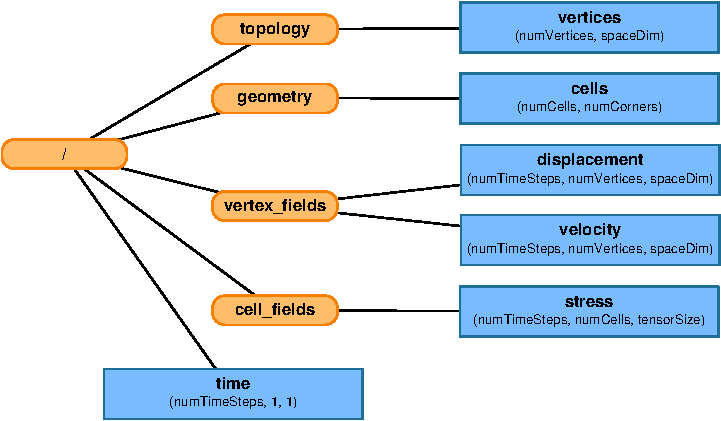
\includegraphics{runpylith/figs/hdf5layout}
  \caption{General layout of a PyLith HDF5 file. The orange rectangles
    with rounded corners identify the groups and the blue rectangles
    with sharp corners identify the datasets. The dimensions of the
    data sets are shown in parentheses. Most HDF5 files will contain
    either \texttt{vertex\_fields} or \texttt{cell\_fields} but not
    both.}
 \label{fig:hdf5:layout}
\end{figure}

See Table \vref{tab:materials:statevars} in Section
\vref{sec:material:parameters} for a table of component values for
tensor output in HDF5 files. To avoid confusion about the ordering of
components for tensor data, we separate the components in the Xdmf
file.

HDF5 files do not contain self-correcting features that allow a file
to be read if part of a dataset is corrupted. This type of error can
occur if a job terminates abnormally in the middle or at the end of a
simulation on a large cluster or other parallel machine. Fortunately,
HDF5 also offers the ability to store datasets in external binary
files with the locations specified by links in the HDF5 file. Note
that the use of external data files results in one data file per
dataset in addition to the HDF5 and Xdmf files. The external data
files use the name of the HDF5 file with the dataset name added to the
pvrefix and the \filename{.h5} suffix replaced by \filename{.dat}. The
HDF5 files include relative paths to the external data files, so these
files can also be moved, but they, too, must be kept together in the
same directory. This provides a more robust method of output because
one can generate an HDF5 file associated with the uncorrupted portions
of the external data files should an error occur. Currently, PyLith
does not include a utility to do this, but we plan to add one in a
future release. Thus, there are two options when writing PyLith output
to HDF5 files: (1) including the datasets directly in the HDF5 files
themselves using the \object{DataWriterHDF5} object or (2) storing the
datasets in external binary files with just metadata in the HDF5 files
using the \object{DataWriterHDF5Ext} object. Both methods provide
similar performance because they will use MPI I/O if it is available.

\warning{Storing the datasets within the HDF5 file in a parallel
  simulation requires that the HDF5 library be configured with the
  \commandline{-{}-enable-parallel} option. The binary PyLith packages
  include this feature and it is a default setting in building HDF5
  via the PyLith Installer.}

Accessing the datasets for additional analysis or visualization is
nearly identical in the two methods because the use of external data
files is completely transparent to the user except for the presence
of the additional files. Note that in order for ParaView to find the
HDF5 and external data files, it must be run from the same relative
location where the simulation was run. For example, if the simulation
was run from a directory called ``work'' and the HDF5/Xdmf files
were written to ``work/output'', then ParaView should be run from
the ``work'' directory. See Table \vref{tab:materials:statevars}
in Section \vref{sec:material:parameters} for a table of component
values for tensor output.

\subsubsection{Parameters}

The parametesr for the \object{DataWriterHDF5} and
\object{DataWriterHDF5Ext} objects is identical:
\begin{inventory}
\propertyitem{filename}{Name of HDF5 file (the Xdmf filename is generated from
the same pvrefix).}
\end{inventory}

An example of changing the writer from the default VTK writer to the
HDF5 writer with external datasets (\object{DataWriterHDF5Ext}) for
output over the domain in a \filename{.cfg} file is
\begin{cfg}
<h>[pylithapp.timedependent.domain.output]</h>
<p>output_freq</p> = time_step
<p>time_step</p> = 1.0*yr
<p>cell_data_fields</p> = [displacement, velocity]
<f>writer</f> = pylith.meshio.DataWriterHDF5Ext
<p>writer.filename</p> = dislocation.h5
\end{cfg}


\subsubsection{HDF5 Utilities}

HDF5 includes several utilities for examining the contents of HDF5
files. \filename{h5dump} is very handy for dumping the hierarchy,
dimensions of datasets, attributes, and even the dataset values to
stdout. 
\begin{shell}
# Dump the entire HDF5 file (not useful for large files).
$$ h5dump mydata.h5
# Dump the hierarchy of an HDF5 file.
$$ h5dump -n mydata.h5
# Dump the hierarchy with dataset dimensions and attributes.
$$ h5dump -H mydata.h5
# Dump dataset 'vertices' in group '/geometry' to stdout.
$$ h5dump -d /geometry/vertices mydata.h5
\end{shell}
We have also include a utility \filename{pylith\_genxdmf} (see Section
\vref{sec:pylith:genxdmf}) that generates an appropriate Xdmf file
from a PyLith HDF5 file. This is very useful if you add fields to
HDF5 files in post-processing and wish to view the results in ParaView
or Visit.


% End of file

\section{Tips and Hints}
\label{sec:tips:hints}

\subsection{Tips and Hints For Running PyLith}
\begin{itemize}
\item Examine the examples for a problem similar to the one you want to
run and dissect it in detail.
\item Start with a uniform-resolution coarse mesh to debug the problem setup.
Increase the resolution as necessary to resolve the solution fields
of interest (resolving stresses/strains may require a higher resolution
than that for resolving displacements).
\item Merge materials using the same material model. This will result in
only one VTK or HDF5 file for each material model rather than several
files.
\item The rate of convergence in quasi-static (implicit) problems can sometimes
be improved by renumbering the vertices in the finite-element mesh
to reduce the bandwidth of the sparse matrix. PyLith can use the reverse
Cuthill-McKee algorithm to reorder the vertices and cells.
\item If you encounter errors or warnings, run \filename{pylithinfo} or use
the \commandline{-{}-help}, \commandline{-{}-help-components}, and \commandline{-{}-help-properties}
command-line arguments when running PyLith to check the parameters
to make sure PyLith is using the parameters you intended.
\item Use the \commandline{-{}-petsc.log\_}view, \commandline{-{}-petsc.ksp\_monitor},
\commandline{-{}-petsc.ksp\_view}, \commandline{-{}-petsc.ksp\_converged\_reason}, and \commandline{-{}-petsc.snes\_converged\_reason}
command-line arguments (or set them in a parameter file) to view PyLith
performance and monitor the convergence.
\item Turn on the journals (see the examples) to monitor the progress of
the code.
\end{itemize}

\subsection{Troubleshooting}
\label{sec:Troubleshooting}

Consult the PyLith FAQ webpage (\url{http://www.geodynamics.org/cig/community/workinggroups/short/workarea/pylith-wiki})
which contains a growing list of common problems and their corresponding
solutions.

\subsubsection{Import Error and Missing Library}
\begin{shell}
ImportError: liblapack.so.2: cannot open shared object file: No such file or directory
\end{shell}

PyLith cannot find one of the libraries. You need to set up your environment
variables (e.g., PATH, PYTHONPATH, and LD\_LIBRARY\_PATH) to match
your installation. If you are using the PyLith binary on Linux or
Mac OS X, run the command \filename{source setup.sh }in the directory
where you unpacked the distribution. This will set up your environment
variables for you. If you are building PyLith from source, please
consult the instructions for building from source.

\subsubsection{Unrecognized Property 'p4wd'}

\begin{shell}
-- pyre.inventory(error) } \\
-- p4wd <- 'true' } \\
-- unrecognized property 'p4wd' } \\
>> command line:: } \\
-- pyre.inventory(error) } \\
-- p4pg <- 'true' } \\
-- unrecognized property ' p4pg'}
\end{shell}
Verify that the filename{mpirun} command included in the PyLith package is
the first one on your PATH: \filename{which mpirun}. If it is not, adjust your PATH environment variable accordingly.

\subsubsection{Detected zero pivor in LU factorization}

\begin{shell}
-- Solving equations.
[0] PETSC ERROR: ----------------
Error Message -------------------------------
[0] PETSC ERROR: Detected zero pivot in LU factorization
see http://www.mcs.anl.gov/petsc/petsc-as/documentation/faq.html\#ZeroPivot!
\end{shell}

This usually occurs when the null space of the system Jacobian is
nonzero, such as the case of a problem without Dirichlet boundary
conditions on any boundary. If this arises when using the split fields
and algebraic multigrid preconditioning, and no additional Dirichlet
boundary conditions are desired, then the workaround is to revert
to using the Additive Schwarz preconditioning without split fields
as discussed in Section \vref{sec:petsc:options}.

\subsubsection{Bus Error}

This often indicates that PyLith is using incompatible versions of
libraries. This can result from changing your environment variables
after configuring or installing PyLith (when building from source) or
from errors in setting the environment variables (\filename{PATH},
\filename{LD\_LIBRARY\_PATH}, and \filename{PYTHONPATH}). If the
former case, simply reconfigure and rebuild PyLith. In the latter
case, check your environment variables (order matters!) to make sure
PyLith finds the desired directories before system directories.

\subsubsection{Segmentation Fault}

A segmentation fault usually results from an invalid read/write to
memory. It might be caused by an error that wasn't trapped or a bug in
the code. Please report these cases so that we can fix these problems
(either trap the error and provide the user with an informative error
message, or fix the bug). If this occurs with any of the problems
distributed with PyLith, simply submit a bug report (see Section
\vref{sec:help}) indicating which problem you ran and your
platform. If the crash occurs for a problem you created, it is a great
help if you can try to reproduce the crash with a very simple problem
(e.g., adjust the boundary conditions or other parameters of one of
the examples to reproduce the segmentation fault). Submit a bug report
along with log files showing the backtrace from a debugger (e.g., gdb)
and the valgrind log file (only available on Linux platforms).  You
can generate a backtrace using the debugger by using the
\commandline{-{}-petsc.start\_in\_debugger} command-line argument:
\begin{shell}
$$ pylith [..args..] --petsc.start_in_debugger
(gdb) continue
(gdb) backtrace
\end{shell}

To use valgrind to detect the memory error, first go to your working
directory and run the problem with \commandline{-{}-launcher.dry}:
\begin{shell}
$$ pylith [..args..] --launcher.dry
\end{shell}

Instead of actually running the problem, this causes PyLith to dump
the mpirun/mpiexec command it will execute. Copy and paste this command
into your shell so you can run it directly. Insert the full path to
valgrind before the full path to mpinemesis and tell valgrind to use
a log file:
\begin{shell}
$$ mpirun /path/to/valgrind --log-file=valgrind-log /path/to/mpinemesis --pyre-start
  [..lots of junk..]
\end{shell}

% End of file

\section{Post-Processing Utilities}

The PyLith distribution includes a few post-processing utilities.
These are Python scripts that are installed into the same bin directory
as the \filename{pylith} executable.


\subsection{\filename{pylith\_eqinfo}}

This utility computes the moment magnitude, seismic moment, seismic
potency, and average slip at user-specified time snapshots from PyLith
fault HDF5 output. The utility works with output from simulations
with either prescribed slip and/or spontaneous rupture. Currently,
we compute the shear modulus from a user-specified spatial database
at the centroid of the fault cells. In the future we plan to account
for lateral variations in shear modulus across the fault when calculating
the seismic moment. The Python script is a Pyre application, so its
parameters can be specified using \filename{.cfg} and command line arguments
just like PyLith. The Pyre properties and facilities include:
\begin{inventory}
\propertyitem{output\_filename}{Filename for output of slip information.}
\propertyitem{faults}{Array of fault names.}
\propertyitem{filename\_pattern}{Filename pattern in C/Python format for creating
filename for each fault. Default is \filename{output/fault\_\%s.h5}.}
\propertyitem{snapshots}{Array of timestamps for slip snapshosts ([-1] means
use last time step in file, which is the default).}
\propertyitem{snapshot\_units}{Units for timestamps in array of snapshots.}
\facilityitem{db\_properties}{Spatial database for elastic properties.}
\facilityitem{coordsys}{Coordinate system associated with mesh in simulation.}
\end{inventory}

\subsection{\filename{pylith\_genxdmf}}
\label{sec:pylith:genxdmf}

This utility generates Xdmf files from HDF5 files that conform to
the layout used by PyLith. It is a simple Python script with a single
command line argument, the HDF5 file for input. Typically, it is used
to regenerate Xdmf files that get corrupted or lost due to renaming
and moving. It is also useful in updating Xdmf files when users add
fields to HDF5 files during post-processing.
\begin{shell}
$$ pylith_genxdmf --file=PYLITH_HDF5_FILE
\end{shell}

\warning{If the HDF5 files contain external datasets, then this
  utility should be run from the same relative path to the HDF5 files
  as when they were created. For example, if a PyLith simulation was
  run from directory \filename{work} and HDF5 files were generated in
  \filename{output/work}, then the utility should be run from the
  directory \filename{work}. Furthermore, a visualization tool, such
  as ParaView, should also be started from the working directory
  \filename{work}.}

% End of file


% End of file


\chapter{Material Models}
\label{cha:material:models}


\section{Specifying Material Properties}

Associating material properties with a given cell involves several
steps. 
\begin{enumerate}
\item In the mesh generation process, assign a material identifier to each
cell.
\item Define material property groups corresponding to each material identifier.
\item Set the parameters for each material group using \filename{.cfg} and/or command-line arguments.
\item Specify the spatial variation in material property parameters using
a spatial database file.
\end{enumerate}

\subsection{Setting the Material Identifier}

Each cell in the finite-element mesh must have a material identifier.
This integer value is associated with a bulk material model. The parameters
of the material model need not be uniform for cells with the same
material identifier. The bulk constitutive model and numerical integration
(quadrature) scheme will, however, be the same for all cells with
the same material identifier value. The material identifier is set
during the mesh generation process. The procedure for assigning this
integer value to a cell depends on the mesh generator. For example,
in the PyLith mesh ASCII format, the identifiers are listed in the
cells group using the material-id data; in CUBIT materials are defined
using blocks; in LaGriT materials are defined by the attribute \texttt{imt1}
and the mregion command.


\subsection{Material Property Groups}

The material property group associates a material model (label for the
material, a bulk constitutive model, and parameters for the
constitutive model) with a material identifier. In previous versions
of PyLith it was necessary to specify containers that defined the
number of groups and associated information for each group. This was
necessary because previous versions of Pyre did not support dynamic
arrays of components, and it was necessary to predefine these
arrays. More recent versions of Pythia do support this, however, and
it is now possible to define material property groups using a
\filename{.cfg} file or on the command-line. User-defined containers
are no longer necessary, and the predefined containers are no longer
available (or necessary). If a set of material groups is not
specified, a single material model is used for the entire problem. See
Sections \vref{sec:Tutorial-3d-hex8} and \vref{sec:Tutorial-3d-tet4}
for examples that demonstrate how to specify more than one material
model.


\subsection{Material Parameters}
\label{sec:material:parameters}

For each material group, there is a single component defining the
material model to be used. The default material model is \object{ElasticIsotropic3D}.
For each material model, the available properties and facilities are:
\begin{inventory}
\propertyitem{id}{This is the material identifier that matches the integer value
assigned to each cell in the mesh generation process.}
\propertyitem{label}{Name or label for the material. This is used in error and
diagnostic reports.}
\facilityitem{db\_properties}{Spatial database specifying the spatial variation
in the parameters of the bulk constitutive model (default is a SimpleDB).}
\facilityitem{db\_initial\_stress}{Spatial database specifying the spatial variation
in the initial stress (default is none).}
\facilityitem{db\_initial\_strain}{Spatial database specifying the spatial variation
in the initial strain (default is none).}
\facilityitem{db\_initial\_state}{Spatial database specifying the spatial variation
in the other initial state variables (default is none).}
\facilityitem{output}{The output manager used for outputting material information.}
\facilityitem{quadrature}{Numerical integration scheme used in integrating fields
over each cell.}
\end{inventory}
An example of setting these parameters in a \filename{.cfg} file for
a problem with two material groups is:
\begin{cfg}
<h>[pylithapp.timedependent]</h>
<p>materials</p> = [elastic,viscoelastic]

<h>[pylithapp.timedependent.materials.elastic]</h>
<p>label</p> = Elastic material
<p>id</p> = 1
<p>db_properties.iohandler.filename</p> = mat\_elastic.spatialdb
<f>quadrature.cell</f> = pylith.feassemble.FIATLagrange
<p>quadrature.cell.dimension</p> = 3

<h>[pylithapp.timedependent.materials.viscoelastic]</h>
<p>label</p> = Viscoelastic material
<p>id</p> = 2
<p>db_properties.iohandler.filename</p> = mat_viscoelastic.spatialdb
<f>quadrature.cell</f> = pylith.feassemble.FIATLagrange
<p>quadrature.cell.dimension</p> = 3
\end{cfg}

These settings correspond to the the problem in Section
\vref{sec:Tutorial-3d-hex8}.  The parameters for the bulk constitutive
models are specified using the spatial databases
\filename{mat\_elastic.spatialdb} and
\filename{mat\_viscoelastic.spatialdb}.  Refer to the discussion of
each material model to find the parameters that must be specified in
the spatial database. Appendix \vref{sec:format:SimpleIOAscii}
describes the format of the SimpleDB spatial database files. In a more
realistic problem, a different spatial database, and possibly a
different material model, would be used for each material group.

In general, we average the output over the quadrature points within
a cell and specify the name of the output files for each material
group:
\begin{cfg}
<h>[pylithapp.timedependent.materials.elastic.output]</h>
<f>cell_filter</f> = pylith.meshio.CellFilterAvg
<p>writer.filename</p> = dislocation-elastic.vtk

<h>[pylithapp.timedependent.materials.viscoelastic.output]</h>
<f>cell_filter</f> = pylith.meshio.CellFilterAvg
<p>writer.filename</p> = dislocation-viscoelastic.vtk
\end{cfg}

These settings again correspond to the problem in Section \vref{sec:Tutorial-3d-hex8}.
The specification of a state variable base filename (\filename{writer.filename}
settings) will cause two files to be created for each material group:
an info file, which describes the material property parameters used
in the model, and a state variables file, which contains the state
variable information. Note that the material property parameters described
by the info file are the parameters used internally by PyLith. In
some cases they are parameters convenient for use in the constitutive
models and are derived from the parameters specified by the user via
the spatial database. If the problem has more than one time step,
a state variable output file will be created for each requested time
step. We have requested that the values be averaged over each cell.
Otherwise, output would be produced for each quadrature point, which
can cause problems with some visualization packages. For this example
problem, the material is three-dimensional isotropic elastic, and
is thus described by three parameters ($\lambda$, $\mu$, $\rho$),
as described below. These properties are output by default. Other
material models require additional parameters, and if users want these
to be output, they must be specified. Similarly, other material models
require state variables in addition to the default stress and strain
variables that are used by all material models. Additional output
may be requested for a material model, as in this example (see Section
\vref{sec:example:twohex8}):
\begin{cfg}
<h>[pylithapp.timedependent.materials.material.output]</h>
<p>cell_data_fields</p> = [total_strain, viscous_strain, stress]
<p>cell_info_fields</p> = [mu, lambda, density, maxwell_time]
\end{cfg}

The properties and state variables available for output in each
material model are listed in Table
\vref{tab:materials:output}. The order of the state variables in
the output arrays is given in Table \vref{tab:materials:statevars}.
For the generalized Maxwell model, values of \texttt{shear\_ratio} and
\texttt{maxwell\_time} are given for each Maxwell element in the model
(there are presently three, as described below). Similarly, there are
three sets of \texttt{viscous\_strain} values for the generalized
Maxwell model.

\begin{table}[htbp]
\caption{Properties and state variables available for output for
  existing material models. Physical properties are available for
  output as \property{cell\_info\_fields} and state variables are
  available for output as \property{cell\_data\_fields}.}
\label{tab:materials:output}

\begin{tabular}{p{1.5in}p{1.8in}p{1.5in}p{1in}}
\textbf{Model} & \textbf{Physical Properties} & \textbf{State Variables} & \textbf{Requires nonlinear solver?}\tabularnewline
\hline 
Elastic & \texttt{mu, lambda, density} & \texttt{total\_strain, stress, cauchy\_stress} & No\\
Maxwell Viscoelastic & \texttt{mu, lambda, density, maxwell\_time} & \texttt{total\_strain,} \texttt{stress, cauchy\_stress, viscous\_strain} & No\\
Generalized Maxwell Viscoelastic & \texttt{mu, lambda, density,} \texttt{shear\_ratio,} \texttt{maxwell\_time} & \texttt{total\_strain, stress, cauchy\_stress, viscous\_strain\_1,} \texttt{viscous\_strain\_2,} \texttt{viscous\_strain\_3} & No\\
Power-law Viscoelastic & \texttt{mu, lambda, density,} \texttt{reference\_strain\_rate, reference\_stress,} 
\texttt{power\_law\_exponent} & \texttt{total\_strain, stress, cauchy\_stress, viscous\_strain} & Yes\\
Drucker-Prager Elastoplastic & \texttt{mu, lambda, density, alpha\_yield},\texttt{ beta, alpha\_flow } & \texttt{total\_strain, stress, cauchy\_stress, plastic\_strain} & Yes\\
\hline 
\end{tabular}
\end{table}

\begin{table}[htbp]
\caption{Order of components in tensor state-variables for material models.}
\label{tab:materials:statevars}
\begin{tabular}{p{2.5in}p{1.5in}p{2.0in}}
\textbf{State Variable} & \textbf{2D} & \textbf{3D}\\
\hline 
\texttt{total\_strain} & $\epsilon_{xx}$, $\epsilon_{yy}$, $\epsilon_{xy}$ & $\epsilon_{xx}$, $\epsilon_{yy}$, $\epsilon_{zz}$, $\epsilon_{xy}$,
$\epsilon_{yz}$, $\epsilon_{xz}$\\
\texttt{stress, cauchy\_stress} & $\sigma_{xx}$, $\sigma_{yy}$, $\sigma_{xy}$ & $\sigma_{xx}$, $\sigma_{yy}$, $\sigma_{zz}$, $\sigma_{xy}$, $\sigma_{yz}$,
$\sigma_{xz}$\\
\texttt{viscous\_strain, plastic\_strain} & $\epsilon_{xx}$, $\epsilon_{yy}$, $\epsilon_{zz}$, $\epsilon_{xy}$ & $\epsilon_{xx}$, $\epsilon_{yy}$, $\epsilon_{zz}$, $\epsilon_{xy}$,
$\epsilon_{yz}$, $\epsilon_{xz}$\\
\texttt{stress4} & $\sigma_{xx}$, $\sigma_{yy}$, $\sigma_{zz}$, $\sigma_{xy}$ & \\
\hline 
\end{tabular}
\end{table}


\subsection{Initial State Variables}
\label{sec:materials:reference:state}

In many problems of interest, the state variables describing a material
model may already have nonzero values prior to the application of
any boundary conditions. For problems in geophysics, the most common
example is a problem that includes the effects of gravitational body
forces. In the real earth, rocks were emplaced and formed under the
influence of gravity. When performing numerical simulations, however,
it is not possible to represent the entire time history of rock emplacement.
Instead, gravity must be ``turned on'' at the beginning of the simulation.
Unfortunately, this results in unrealistic amounts of deformation
at the beginning of a simulation. An alternative is to provide initial
state variables for the region under consideration. This allows the
specification of a set of state variables that is consistent with
the prior application of gravitational body forces. In a more general
sense, initial values for state variables may be used to provide values
that are consistent with any set of conditions that occurred prior
to the beginning of a simulation. The current release of PyLith allows
the specification of initial stresses, strains, and state variables
for all materials; however, not all of the initial state variables
are presently used. For example, \texttt{cauchy\_stress} is available
as a state variable for all materials, but specifying an initial value
would not make sense for most problems.


\subsubsection{Specification of Initial State Variables}

State variables are specific to a given material, so initial values
for state variables are specified as part of the material description.
The default is that no initial state variables are specified. In computing
the elastic prestep, appropriate values for the state variables are
set; otherwise the state variables are set to zero. To override this
behavior, specify a spatial database for the initial stress, strain,
and/or state variables as in the example from the tutorial in Section
\vref{sec:Tutorial-3d-hex8}:
\begin{cfg}
<h>[pylithapp.timedependent.materials.elastic]</h>
<f>db_initial_stress</f> = spatialdata.spatialdb.SimpleDB
<p>db_initial_stress.iohandler.filename<p> = initial\_stress.spatialdb
\end{cfg}

\warning{Using the elastic prestep with initial state variables will
  generally lead to the state variables being ignored (the initial out
  of plane stress is the exception), because the elastic prestep will
  set the state variables based on the elastic solution.}

\warning{Currently, PyLith assumes initial displacements and
  velocities of zero, so any initial strain and state variables should
  be consistent with these initial conditions.  This limitation will
  be removed in future releases.}

As mentioned in section \vref{sec:materials:formulations:viscoelastic}, plane
strain problems do not include the out-of-plane stress component ($\sigma_{zz}$),
and an additional state variable (\texttt{stress-zz-initial}) is provided
for all two-dimensional viscoelastic and elastoplastic models. To
completely specify the initial stresses, the user must provide two
spatial databases: an initial stress database that includes the three
2D stress components ($\sigma_{xx}$, $\sigma_{yy}$, and $\sigma_{xy}$)
and an additional database containing the out of plane stress and
initial values for all other state variables for the given material.
The complete initial stress field may then be defined in the \filename{.cfg}
file as:
\begin{cfg}
<h>[pylithapp.problem.materials.powerlaw]</h>
# First specify initial 2D stresses
<f>db_initial_stress</f> = spatialdata.spatialdb.SimpleDB
<p>db_initial_stress.label</p> = 2D initial stress
<p>db_initial_stress.iohandler.filename</p> = inititial_stress_2d.spatialdb

# Now specify out-of-plane initial stresses (and all other state variables)
<f>db_initial_state</f> = spatialdata.spatialdb.SimpleDB
<p>db_initial_state.label</p> = Out of plane strain initial stress
<p>db_initial_state.iohandler.filename</p> = initial_state_2d.spatialdb
\end{cfg}

\begin{table}[htbp]
\caption{Values in spatial database for initial state variables for 3D
  problems.  2D problems use only the relevant values. Note that
  initial stress and strain are available for all material
  models. Some models have additional state variables (Table
  \vref{tab:materials:output}) and initial values for these may
  also be provided.}
\begin{tabular}{p{0.85in}p{5.0in}}
\textbf{State Variable} & \textbf{Values in Spatial Database}\\
\hline 
initial stress & \texttt{stress-xx, stress-yy, stress-zz, stress-xy, stress-yz, stress-xz}\\
initial strain & \texttt{total-strain-xx, total-strain-yy, total-strain-zz, total-strain-xy,
total-strain-yz, total-strain-xz}\\
\hline 
\end{tabular}
\end{table}


\subsection{Cauchy Stress Tensor and Second Piola-Kirchoff Stress Tensor}

In outputting the stress tensor (see Tables
\vref{tab:materials:output} and \vref{tab:materials:statevars}),
the tensor used internally in the formulation of the governing
equation is the \texttt{stress} field available for output. For the
infinitesimal strain formulation this is the Cauchy stress tensor; for
the finite strain formulation, this is the second Piola-Kirchoff
stress tensor. The user may also explicitly request output of the
Cauchy stress tensor (\texttt{cauchy\_stress} field). Obviously, this
is identical to the \texttt{stress} field when using the infinitesimal
strain formulation.  See section \vref{sec:small:strain:formulation}
for a discussion of the relationship between the Cauchy stress tensor
and the second Piola-Kirchhoff stress tensor.

\important{Although the second Piola-Kirchoff stress tensor has little
  physical meaning, the second Piola-Kirchoff stress tensor (not the
  Cauchy stress tensor) values should be specified in the initial
  stress database when using the finite strain formulation.}

\subsection{Stable time step}
\label{sec:stable:time:step}

PyLith computes the stable time step in both quasi-static and dynamic
simulations. In quasi-static simulations the stability of the implicit
time stepping scheme does not depend on the time step; instead, the
stable time step is associated with the accuracy of the solution.  For
viscoelastic materials the stable time step uses 1/5 of the minimum
viscoelastic relaxation time. In purely elastic materials, the
accuracy is independent of the time step, so the stable time step is
infinite.  The same is true for elastoplastic materials, since there
is no inherent time scale for these problems. Depending on the loading
rate, however, it is possible to impose a load increment that is large
enough so that the resulting solution may be inaccurate or divergent.
In quasi-static simulations we recompute the stable time step at every
time step.

\warning{Caution must be used in assigning time step sizes for
  elastoplastic problems, and the linear and nonlinear convergence
  should be monitored closely.}

In dynamic simulations the stability of the explicit time-stepping
scheme integration does depend on the time step via the Courant-Friderichs-Lewy
condition \cite{Courant:etal:1967}. This condition states that the
critical time step is the time it takes for the P wave to travel across
the shortest dimension of a cell. In most cases this is the shortest
edge length. However, distorted cells which have relatively small
areas in 2-D or relatively small volumes in 3-D for the given edge
lengths also require small time steps due to the artificially high
stiffness associated with the distorted shape. As a result, we set
the stable time step to be the smaller of the shortest edge length
and a scaling factor times the radius of an inscribed circle (in 2-D),
\begin{gather}
dt=\min(e_{\mathit{min}},3.0r_{inscribed})\\
r_{inscribed}=\sqrt{\frac{k(k-e_{0})(k-e_{1})(k-e_{2})}{k}}\\
k=\frac{1}{2}(e_{0}+e_{1}+e_{2})
\end{gather}
and sphere (in 3-D),
\begin{gather}
dt=\min(e_{\mathit{min}},6.38r_{inscribed})\\
r_{inscribed}=3V/(A_{0}+A_{1}+A_{2}+A_{3}),
\end{gather}
where $e_{i}$ denotes the length of edge $i$, $A_{i}$ denotes the
area of face $i$, and $V$ is the volume of the cell. We determined
the scaling factoring empirically using several benchmarks. In dynamic
simulations we check the stable time step only at the beginning of
the simulation. That is, we assume the elastic properties and mesh
do not change, so that the stable time step is constant throughout
the simulation.

The stable time step is used in all three of the time stepping schemes
used by PyLith (see section \vref{sec:time-stepping}). In general,
an error is generated if the user attempts to use a time step size
larger than the stable time step. The stable time steps for each cell
can be included in the output with the other \property{cell\_info\_fields}.
For implicit time stepping the field is \texttt{stable\_dt\_implicit}
and for explicit time stepping the field is \texttt{stable\_dt\_explicit}.


\section{Elastic Material Models}

The generalized form of Hooke's law relating stress and strain for
linear elastic materials is

\begin{gather}
\sigma_{ij}=C_{ijkl}\left(\epsilon_{kl}-\epsilon_{kl}^{I}\right)+\sigma_{ij}^{I}\,,\label{eq:1}
\end{gather}
where we have included both initial strains and initial stresses,
denoted with the superscript \textsl{I}. Due to symmetry considerations,
however, the 81 components of the elasticity matrix are reduced to
21 independent components for the most general case of anisotropic
elasticity. Representing the stress and strain in terms of vectors,
the constitutive relation may be written
\begin{gather}
\overrightarrow{\sigma}=\underline{C}\left(\vec{\epsilon}-\vec{\epsilon}^{I}\right)+\vec{\sigma}^{I},\label{eq:2}
\end{gather}
where

\begin{gather}
\underline{C}=\left[\begin{array}{cccccc}
C_{1111} & C_{1122} & C_{1133} & C_{1112} & C_{1123} & C_{1113}\\
C_{1122} & C_{2222} & C_{2233} & C_{2212} & C_{2223} & C_{2213}\\
C_{1133} & C_{2233} & C_{3333} & C_{3312} & C_{3323} & C_{3313}\\
C_{1112} & C_{2212} & C_{3312} & C_{1212} & C_{1223} & C_{1213}\\
C_{1123} & C_{2223} & C_{3323} & C_{1223} & C_{2323} & C_{2313}\\
C_{1113} & C_{2213} & C_{3313} & C_{1213} & C_{2313} & C_{1313}
\end{array}\right]\:.\label{eq:3}
\end{gather}
For the case of isotropic elasticity, the number of independent components
reduces to two, and the model can be characterized by two parameters,
Lame's constants $\mu$ and $\lambda$. Lame's constants are related
to the density ($\rho$), shear wave speed ($v_{s}$), and compressional
wave speed ($v_{p}$) via
\begin{equation}
\begin{aligned}\mu= & \rho v_{s}^{2}\\
\lambda= & \rho v_{p}^{2}-2\mu
\end{aligned}
\label{eq:4}
\end{equation}

\begin{table}[htbp]
  \caption{Values in spatial databases for the elastic material
    constitutive models.}
\begin{tabular}{lll}
\textbf{Spatial database} & \textbf{Value} & \textbf{Description}\\
\hline 
\facility{db\_properties} & \texttt{vp} & Compressional wave speed, $v_{p}$\\
 & \texttt{vs} & Shear wave speed, $v_{s}$\\
 & \texttt{density} & Density, $\rho$\\
\facility{db\_initial\_stress} & \texttt{stress-xx}, \ldots & Initial stress components\\
\facility{db\_initial\_strain} & \texttt{total-strain-xx}, \ldots & Initial strain components\\
\hline 
\end{tabular}
\end{table}


\subsection{2D Elastic Material Models}

In 2D we can write Hooke's law as
\begin{gather}
\left[\begin{array}{c}
\sigma_{11}\\
\sigma_{22}\\
\sigma_{12}
\end{array}\right]=\left[\begin{array}{ccc}
C_{1111} & C_{1122} & C_{1112}\\
C_{1122} & C_{2222} & C_{2212}\\
C_{1112} & C_{2212} & C_{1212}
\end{array}\right]\left[\begin{array}{c}
\epsilon_{11}-\epsilon_{11}^{I}\\
\epsilon_{22}-\epsilon_{22}^{I}\\
\epsilon_{12}-\epsilon_{12}^{I}
\end{array}\right]+\left[\begin{array}{c}
\sigma_{11}^{I}\\
\sigma_{22}^{I}\\
\sigma_{12}^{I}
\end{array}\right]\:.\label{eq:9}
\end{gather}


\subsubsection{Elastic Plane Strain}

If the gradient in deformation with respect to the $x_{3}$ axis is
zero, then $\epsilon_{33}=\epsilon_{13}=\epsilon_{23}=0$ and plane
strain conditions apply, so we have 
\begin{gather}
\left[\begin{array}{c}
\sigma_{11}\\
\sigma_{22}\\
\sigma_{12}
\end{array}\right]=\left[\begin{array}{ccc}
\lambda+2\mu & \lambda & 0\\
\lambda & \lambda+2\mu & 0\\
0 & 0 & 2\mu
\end{array}\right]\left[\begin{array}{c}
\epsilon_{11}-\epsilon_{11}^{I}\\
\epsilon_{22}-\epsilon_{22}^{I}\\
\epsilon_{12}-\epsilon_{12}^{I}
\end{array}\right]+\left[\begin{array}{c}
\sigma_{11}^{I}\\
\sigma_{22}^{I}\\
\sigma_{12}^{I}
\end{array}\right]\:.\label{eq:10}
\end{gather}


\subsubsection{Elastic Plane Stress}

If the $x_{1}x_{2}$ plane is traction free, then $\sigma_{33}=\sigma_{13}=\sigma_{23}=0$
and plane stress conditions apply, so we have
\begin{gather}
\left[\begin{array}{c}
\sigma_{11}\\
\sigma_{22}\\
\sigma_{12}
\end{array}\right]=\left[\begin{array}{ccc}
\frac{4\mu(\lambda+\mu)}{\lambda+2\mu} & \frac{2\mu\lambda}{\lambda+2\mu} & 0\\
\frac{2\mu\lambda}{\lambda+2} & \frac{4\mu(\lambda+\mu)}{\lambda+2\mu} & 0\\
0 & 0 & 2\mu
\end{array}\right]\left[\begin{array}{c}
\epsilon_{11}-\epsilon_{11}^{I}\\
\epsilon_{22}-\epsilon_{22}^{I}\\
\epsilon_{12}-\epsilon_{12}^{I}
\end{array}\right]+\left[\begin{array}{c}
\sigma_{11}^{I}\\
\sigma_{22}^{I}\\
\sigma_{12}^{I}
\end{array}\right]\:,\label{eq:11}
\end{gather}
where
\begin{equation}
\begin{gathered}\epsilon_{33}=-\frac{\lambda}{\lambda+2\mu}(\epsilon_{11}+\epsilon_{22})+\epsilon_{33}^{I}\\
\epsilon_{13}=\epsilon_{23}=0\,.
\end{gathered}
\label{eq:12}
\end{equation}

\subsection{3D Elastic Material Models}

\subsubsection{Isotropic}

For this case the stress-strain matrix, $\underline{C}$, becomes
\begin{gather}
\underline{C}=\left[\begin{array}{cccccc}
\lambda+2\mu & \lambda & \lambda & 0 & 0 & 0\\
\lambda & \lambda+2\mu & \lambda & 0 & 0 & 0\\
\lambda & \lambda & \lambda+2\mu & 0 & 0 & 0\\
0 & 0 & 0 & 2\mu & 0 & 0\\
0 & 0 & 0 & 0 & 2\mu & 0\\
0 & 0 & 0 & 0 & 0 & 2\mu
\end{array}\right]\:.\label{eq:13}
\end{gather}


\section{Viscoelastic Materials}
\label{sec:materials:viscoelastic}

At present, there are six viscoelastic material models available in
PyLith (Table \vref{tab:materials:viscoelastic} and Figure
\vref{fig:material:models}). Future code versions may include alternative
formulations for the various material models (Appendix \vref{cha:materials:alternative:formulations}),
so that users may use the most efficient formulation for a particular
problem. Note that both 2D and 3D viscoelastic models are described,
but we present below only the 3D formulations. The 2D formulations
are easily obtained from the plane strain definition. The one aspect
of the 2D formulations that is different is the specification of initial
stresses. Since 2D models only have three tensor components, it is
not possible to specify the normal stress in the out-of-plane direction
($\sigma_{33}$), which is generally nonzero, using the same method
as the other tensor components. To allow for the specification of
this initial stress component, an additional state variable corresponding
to $\sigma_{33}^{I}$ is provided (\texttt{stress\_zz\_initial}).
This state variable is provided for all of the viscoelastic material
models as well as the plane strain Drucker-Prager elastoplastic model.
See section \vref{sec:materials:reference:state} for additional information
on specifying initial stresses for plane strain problems. For the
PowerLawPlaneStrain model, all four of the stress components are needed,
so a 4-component stress state variable (\texttt{stress4}) is provided
in addition to the normal 3-component \texttt{stress} state variable
(see Table \vref{tab:materials:output}).

\begin{table}[htbp]
\caption{Available viscoelastic materials
for PyLith.}
\label{tab:materials:viscoelastic}
\begin{tabular}{p{1.5in}p{4.5in}}
\textbf{Model Name} & \textbf{Description}\\
\hline 
\object{MaxwellPlaneStrain} & Plane strain Maxwell material with linear viscous rheology\\
\object{GenMaxwellPlaneStrain} & Plane strain generalized Maxwell material (3 Maxwell models in parallel)\\
\object{PowerLawPlaneStrain} & Plane strain Maxwell material with power-law viscous rheology\\
\object{MaxwellIsotropic3D} & Isotropic Maxwell material with linear viscous rheology\\
\object{GenMaxwellIsotropic3D} & Generalized model consisting of 3 Maxwell models in parallel\\
\object{PowerLaw3D} & Isotropic Maxwell material with power-law viscous rheology\\
\hline 
\end{tabular}
\end{table}

\begin{figure}[htbp]
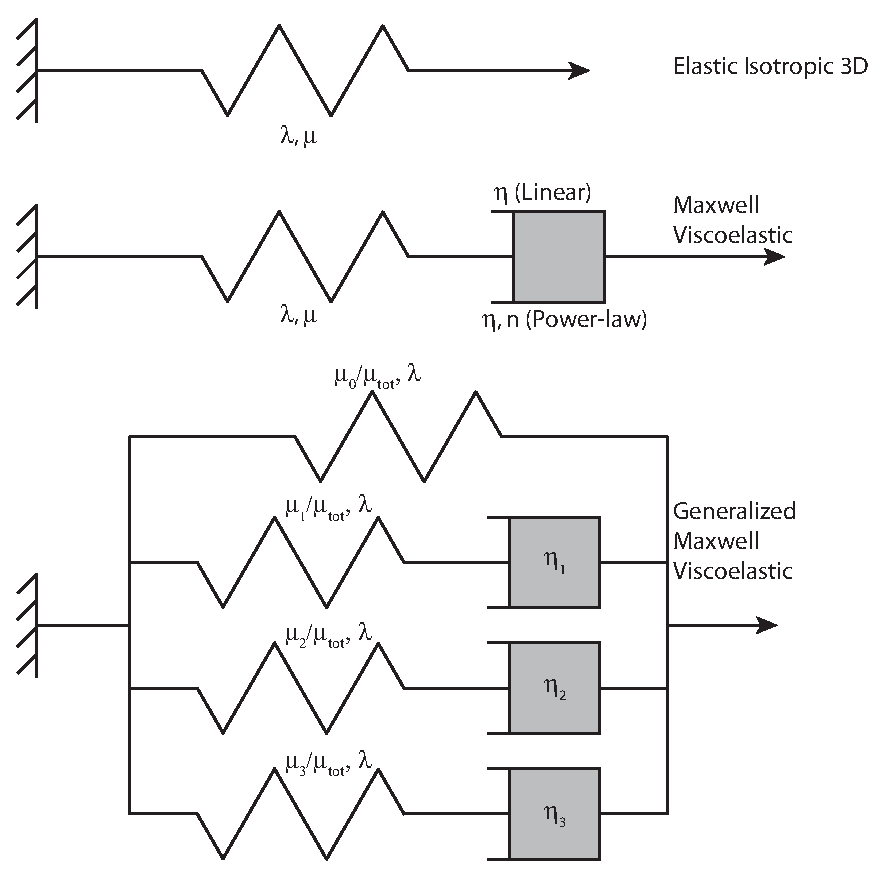
\includegraphics[scale=0.75]{materials/figs/pylith-materials}
\caption{Spring-dashpot 1D representations of the available 3D elastic
  and 2D/3D viscoelastic material models for PyLith.  The top model is
  a linear elastic model, the middle model is a Maxwell model, and the
  bottom model is a generalized Maxwell model. For the generalized
  Maxwell model, $\lambda$ and $\mu_{tot}$ are specified for the
  entire model, and then the ratio $\mu_{i}/\mu_{tot}$ is specified
  for each Maxwell model. For the power-law model, the linear dashpot
  in the Maxwell model is replaced by a nonlinear dashpot obeying a
  power-law.}
\label{fig:material:models}
\end{figure}


\subsection{Definitions}

In the following sections, we use a combination of vector and index
notation (our notation conventions are shown in Table \vref{tab:notation}).
When using index notation, we use the common convention where repeated
indices indicate summation over the range of the index. We also make
frequent use of the scalar inner product. The scalar inner product
of two second-order tensors may be written
\begin{gather}
\underline{a}\cdot\underline{b}=a_{ij}b_{ij}\,.\label{eq:14}
\end{gather}
Although the general constitutive relations are formulated in terms
of the stress and strain, we frequently make use of the deviatoric
stress and strain in our formulation. We first define the mean stress,
$P$, and mean strain, $\theta$:
\begin{gather}
P=\frac{\sigma_{ii}}{3}\,,\,\,\,\,\theta=\frac{\epsilon_{ii}}{3}\,,\label{eq:15}
\end{gather}
where the $\sigma_{ii}$ and $\epsilon_{ii}$ represent the trace
of the stress and strain tensors, respectively. We then define the
deviatoric components of stress and strain as
\begin{gather}
S_{ij}=\sigma_{ij}-P\delta_{ij}\,,\,\,\,\, e_{ij}=\epsilon_{ij}-\theta\delta_{ij}\,,\label{eq:16}
\end{gather}
where $\delta_{ij}$ is the Kronecker delta. Using the deviatoric
components, we define the effective stress, $\overline{\sigma}$,
the second deviatoric stress invariant, $J_{2}^{\prime}$, the effective
deviatoric strain, $\overline{e}$, and the second deviatoric strain
invariant, $L_{2}^{\prime}$, as
\begin{gather}
\overline{\sigma}=\sqrt{\frac{3}{2}\underline{S}\cdot\underline{S}}\,\,\nonumber \\
J_{2}^{\prime}=\frac{1}{2}\underline{S}\cdot\underline{S}\,.\label{eq:17}\\
\overline{e}=\sqrt{\frac{2}{3}\underline{e}\cdot\underline{e}}\,\,\nonumber \\
L_{2}^{\prime}=\frac{1}{2}\underline{e}\cdot\underline{e}\,\,\nonumber 
\end{gather}
Due to the symmetry of the stress and strain tensors, it is sometimes
convenient to represent them as vectors:
\begin{gather}
\overrightarrow{\sigma^{T}}=\left[\begin{array}{cccccc}
\sigma_{11} & \sigma_{22} & \sigma_{33} & \sigma_{12} & \sigma_{23} & \sigma_{31}\end{array}\right]\label{eq:18}\\
\overrightarrow{\epsilon^{T}}=\left[\begin{array}{cccccc}
\epsilon_{11} & \epsilon_{22} & \epsilon_{33} & \epsilon_{12} & \epsilon_{23} & \epsilon_{31}\end{array}\right]\:.\nonumber 
\end{gather}
Note that when taking the scalar inner product of two tensors represented
as vectors, it is necessary to double the products representing off-diagonal
terms.

For quantities evaluated over a specific time period, we represent
the initial time as a prefixed subscript and the end time as a prefixed
superscript. In cases where the initial time does not appear, it is
understood to be $-\infty$.

\subsection{Linear Viscoelastic Models}

Linear viscoelastic models are obtained by various combinations of
a linear elastic spring and a linear viscous dashpot in series or
parallel. The simplest example is probably the linear Maxwell model,
which consists of a spring in series with a dashpot, as shown in Figure
\vref{fig:material:models}. For a one-dimensional model, the response
is given by
\begin{equation}
\frac{d\epsilon_{Total}}{dt}=\frac{d\epsilon_{D}}{dt}+\frac{d\epsilon_{S}}{dt}=\frac{\sigma}{\eta}+\frac{1}{E}\frac{d\sigma}{dt}\:,
\end{equation}
where $\epsilon_{Total}$ is the total strain, $\epsilon_{D}$ is
the strain in the dashpot, $\epsilon_{S}$ is the strain in the spring,
$\sigma$ is the stress, $\eta$ is the viscosity of the dashpot,
and $E$ is the spring constant. When a Maxwell material is subjected
to constant strain, the stresses relax exponentially with time. When
a Maxwell material is subjected to a constant stress, there is an
immediate elastic strain, corresponding to the response of the spring,
and a viscous strain that increases linearly with time. Since the
strain response is unbounded, the Maxwell model actually represents
a fluid.

Another simple model is the Kelvin-Voigt model, which consists of
a spring in parallel with a dashpot. In this case, the one-dimensional
response is given by
\begin{equation}
\sigma\left(t\right)=E\epsilon\left(t\right)+\eta\frac{d\epsilon\left(t\right)}{dt}\:.
\end{equation}
As opposed to the Maxwell model, which represents a fluid, the Kelvin-Voigt
model represents a solid undergoing reversible, viscoelastic strain.
If the material is subjected to a constant stress, it deforms at a
decreasing rate, gradually approaching the strain that would occur
for a purely elastic material. When the stress is released, the material
gradually relaxes back to its undeformed state.

The most general form of linear viscoelastic model is the generalized
Maxwell model, which consists of a spring in parallel with a number
of Maxwell models (see Figure \vref{fig:material:models}). Using this
model, it is possible to represent a number of simpler viscoelastic
models. For example, a simple Maxwell model is obtained by setting
the elastic constants of all springs to zero, with the exception of
the spring contained in the first Maxwell model ($\mu_{1}$). Similarly,
the Kelvin-Voigt model may be obtained by setting the elastic constants
$\mu_{2}=\mu_{3}=0$, and setting $\mu_{1}=\infty$ (or a very large
number).


\subsection{Formulation for Generalized Maxwell Models}
\label{sec:materials:formulation:generalized:Maxwell}

As described above, the generalized Maxwell viscoelastic model consists
of a number of Maxwell linear viscoelastic models in parallel with
a spring, as shown in Figure \vref{fig:material:models}. PyLith includes
the specific case of a spring in parallel with three Maxwell models.
As described in the previous paragraph, a number of common material
models may be obtained from this model by setting the shear moduli
of various springs to zero or infinity (or a large number), such as
the Maxwell model, the Kelvin model, and the standard linear solid.
We follow formulations similar to those used by Zienkiewicz and Taylor
\cite{Zienkiewicz:Taylor:2000} and Taylor \cite{Taylor:2003}. In
this formulation, we specify the total shear modulus of the model
($\mu_{tot}$) and Lame's constant ($\lambda$). We then provide the
fractional shear modulus for each Maxwell element spring in the model.
It is not necessary to specify the fractional modulus for $\mu_{0}$,
since this is obtained by subtracting the sum of the other ratios
from 1. Note that the sum of all these fractions must equal 1. We
use a similar formulation for our linear Maxwell viscoelastic model,
but in that case $\mu_{0}$ is always zero and we only use a single
Maxwell model. The parameters defining the standard Maxwell model
are shown in Table \vref{tab:materials:linear:Maxwell}, and those defining the
generalized Maxwell model are shown in Table \vref{tab:materials:generalized:Maxwell}.

As for all our viscoelastic models, the volumetric strain is completely
elastic, and the viscoelastic deformation may be expressed purely
in terms of the deviatoric components:
\begin{equation}
\underline{S}=2\mu_{tot}\left[\mu_{0}\underline{e}+\sum_{i=1}^{N}\mu_{i}\underline{q}^{i}-\underline{e}^{I}\right]+\underline{S}^{I}\,;\; P=3K\left(\theta-\theta^{I}\right)+P^{I}\,,\label{eq:19}
\end{equation}
where \textsl{K} is the bulk modulus, $N$ is the number of Maxwell
models, and the variable $\underline{q}^{i}$ follows the evolution
equations
\begin{equation}
\underline{\dot{q}}^{i}+\frac{1}{\tau_{i}}\underline{q}^{i}=\underline{\dot{e}}.\label{eq:20}
\end{equation}
The $\tau_{i}$ are the relaxation times for each Maxwell model:
\begin{equation}
\tau_{i}=\frac{\eta_{i}}{\mu_{tot}\mu_{i}}\:.\label{eq:21-1}
\end{equation}

An alternative to the differential equation form above is an integral
equation form expressed in terms of the relaxation modulus function.
This function is defined in terms of an idealized experiment in which,
at time labeled zero ($t=0$), a specimen is subjected to a constant
strain, $\underline{e}_{0}$, and the stress response, $\underline{S}\left(t\right)$,
is measured. For a linear material we obtain:
\begin{equation}
\underline{S}\left(t\right)=2\mu\left(t\right)\left(\underline{e}_{0}-\underline{e}^{I}\right)+\underline{S}^{I}\,,\label{eq:21}
\end{equation}
where $\mu\left(t\right)$ is the shear relaxation modulus function.
Using linearity and superposition for an arbitrary state of strain
yields an integral equation:
\begin{equation}
\underline{S}\left(t\right)=\intop_{-\infty}^{t}\mu\left(t-T\right)\underline{\dot{e}}\, dT\,.\label{eq:22}
\end{equation}
If we assume the modulus function in Prony series form we obtain
\begin{equation}
\mu\left(t\right)=\mu_{tot}\left(\mu_{0}+\sum_{i=1}^{N}\mu_{i}\exp\frac{-t}{\tau_{i}}\right)\,,\label{eq:23}
\end{equation}
where
\begin{equation}
\mu_{0}+\sum_{i=1}^{N}\mu_{i}=1\,.\label{eq:24}
\end{equation}
With the form in Equation \vref{eq:23}, the integral equation form
is identical to the differential equation form.

If we assume the material is undisturbed until a strain is suddenly
applied at time zero, we can divide the integral into
\begin{equation}
\intop_{-\infty}^{t}\left(\cdot\right)\, dT=\intop_{-\infty}^{0^{-}}\left(\cdot\right)\, dT+\intop_{0^{-}}^{0^{+}}\left(\cdot\right)\, dT+\intop_{0^{+}}^{t}\left(\cdot\right)\, dT\,.\label{eq:27}
\end{equation}
The first term is zero, the second term includes a jump term associated
with $\underline{e}_{0}$ at time zero, and the last term covers the
subsequent history of strain. Applying this separation to Equation
\vref{eq:22},
\begin{equation}
\underline{S}\left(t\right)=2\mu\left(t\right)\left(\underline{e}_{0}-\underline{e}^{I}\right)+\underline{S}^{I}+2\int_{0}^{t}\mu\left(t-T\right)\underline{\dot{e}}\left(T\right)\, dT\,,\label{eq:28}
\end{equation}
where we have left the sign off of the lower limit on the integral.

Substituting Equation \vref{eq:23} into \vref{eq:28}, we obtain
\begin{equation}
\underline{S}\left(t\right)=2\mu_{tot}\left\{ \mu_{0}\underline{e}\left(t\right)+\sum_{i=1}^{N}\left[\mu_{i}\exp\frac{-t}{\tau_{i}}\left(\underline{e}_{0}+\intop_{0}^{t}\exp\frac{t}{\tau_{i}}\underline{\dot{e}}\left(T\right)\, dT\right)\right]-\underline{e}^{I}\right\} +\underline{S}^{I}\,.\label{eq:29}
\end{equation}
We then split each integral into two ranges: from 0 to $t_{n}$, and
from $t_{n}$ to $t$, and define each integral as
\begin{equation}
\underline{i}_{i}^{1}\left(t\right)=\intop_{0}^{t}\exp\frac{T}{\tau_{i}}\underline{\dot{e}}\left(T\right)\, dT\,.\label{eq:30}
\end{equation}
The integral then becomes
\begin{equation}
\underline{i}_{i}^{1}\left(t\right)=\underline{i}_{i}^{1}\left(t_{n}\right)+\intop_{t_{n}}^{t}\exp\frac{T}{\tau_{i}}\underline{\dot{e}}\left(T\right)\, dT\,.\label{eq:31}
\end{equation}
Including the negative exponential multiplier:
\begin{equation}
\underline{h}_{i}^{1}\left(t\right)=\exp\frac{-t}{\tau_{i}}\underline{i}_{i}^{1}\,.\label{eq:32}
\end{equation}
Then
\begin{equation}
\underline{h}_{i}^{1}\left(t\right)=\exp\frac{-\Delta t}{\tau_{i}}\underline{h}_{i}^{1}\left(t_{n}\right)+\Delta\underline{h}_{i}\,,\label{eq:33}
\end{equation}
where
\begin{equation}
\Delta\underline{h}_{i}=\exp\frac{-t}{\tau_{i}}\intop_{t_{n}}^{t}\exp\frac{T}{\tau_{i}}\underline{\dot{e}}\left(T\right)\, dT\,.\label{eq:34}
\end{equation}
Approximating the strain rate as constant over each time step, the
solution may be found as
\begin{equation}
\Delta\underline{h}_{i}=\frac{\tau_{i}}{\Delta t}\left(1-\exp\frac{-\Delta t}{\tau_{i}}\right)\left(\underline{e}-\underline{e}_{n}\right)=\Delta h_{i}\left(\underline{e}-\underline{e}_{n}\right)\,.\label{eq:35}
\end{equation}
The approximation is singular for zero time steps, but a series expansion
may be used for small time-step sizes:
\begin{equation}
\Delta h_{i}\approx1-\frac{1}{2}\left(\frac{\Delta t}{\tau_{i}}\right)+\frac{1}{3!}\left(\frac{\Delta t}{\tau_{i}}\right)^{2}-\frac{1}{4!}\left(\frac{\Delta t}{\tau_{i}}\right)^{3}+\cdots\,.\label{eq:36}
\end{equation}
This converges with only a few terms. With this formulation, the constitutive
relation now has the simple form:
\begin{equation}
\underline{S}\left(t\right)=2\mu_{tot}\left(\mu_{0}\underline{e}\left(t\right)+\sum_{i=1}^{N}\mu_{i}\underline{h}_{i}^{1}\left(t\right)-\underline{e}^{I}\right)+\underline{S}^{I}\,.\label{eq:37}
\end{equation}


We need to compute the tangent constitutive matrix when forming the
stiffness matrix. In addition to the volumetric contribution to the
tangent constitutive matrix, we require the deviatoric part:
\begin{equation}
\frac{\partial\underline{S}}{\partial\underline{\epsilon}}=\frac{\partial\underline{S}}{\partial\underline{e}}\frac{\partial\underline{e}}{\partial\underline{\epsilon}}\,,\label{eq:38}
\end{equation}
where the second derivative on the right may be easily deduced from
Equation \vref{eq:16}. The other derivative is given by
\begin{equation}
\frac{\partial\underline{S}}{\partial\underline{e}}=2\mu_{tot}\left[\mu_{0}\underline{I}+\sum_{i=1}^{N}\mu_{i}\frac{\partial\underline{h}_{i}^{1}}{\partial\underline{e}}\right]\,,\label{eq:39}
\end{equation}
where $\underline{I}$ is the identity matrix. From Equations \vref{eq:33}
through \vref{eq:35}, the derivative inside the brackets is
\begin{equation}
\frac{\partial\underline{h}_{i}^{1}}{\partial\underline{e}}=\Delta h_{i}\left(\Delta t\right)\underline{I}\,.\label{eq:40}
\end{equation}
The complete deviatoric tangent relation is then
\begin{equation}
\frac{\partial\underline{S}}{\partial\underline{\epsilon}}=2\mu_{tot}\left[\mu_{0}+\sum_{i=1}^{N}\mu_{i}\Delta h_{i}\left(\Delta t\right)\right]\frac{\partial\underline{e}}{\partial\underline{\epsilon}}\,.\label{eq:41}
\end{equation}


We use this formulation for both our Maxwell and generalized Maxwell
viscoelastic models. For the Maxwell model, $\mu_{0}=0$ and $N=1$.
For the generalized Maxwell model, $N=3.$ The stable time step is
equal to 1/5 of the minimum relaxation time for all of the Maxwell
models (equation \vref{eq:21-1}).

\begin{table}[htbp]
\caption{Values in spatial databases for the linear Maxwell viscoelastic material constitutive model.}
\label{tab:materials:linear:Maxwell}
\begin{tabular}{lll}
\textbf{Spatial database} & \textbf{Value} & \textbf{Description}\\
\hline 
\facility{db\_properties} & \texttt{vp} & Compressional wave speed, $v_{p}$\\
 & \texttt{vs} & Shear wave speed, $v_{s}$\\
 & \texttt{density} & Density, $\rho$\\
 & \texttt{viscosity} & Viscosity, $\eta$\\
\facility{db\_initial\_stress} & \texttt{stress-xx}, \ldots & Initial stress components\\
\facility{db\_initial\_strain} & \texttt{total-strain-xx}, \ldots & Initial strain components\\
\facility{db\_initial\_state} & \texttt{viscous-strain-xx}, \ldots & Initial viscous strain components\\
 & \texttt{stress-zz-initial} & Initial out-of-plane stress (2D only)\\
\hline 
\end{tabular}
\end{table}

\begin{table}[htbp]
\caption{Values in spatial database used as parameters in the
  generalized linear Maxwell viscoelastic material constitutive
  model.}
\label{tab:materials:generalized:Maxwell}
\begin{tabular}{lll}
\textbf{Spatial database} & \textbf{Value} & \textbf{Description}\\
\hline 
\facility{db\_properties} & \texttt{vp} & Compressional wave speed, $v_{p}$\\
 & \texttt{vs} & Shear wave speed, $v_{s}$\\
 & \texttt{density} & Density, $\rho$\\
 & \texttt{shear-ratio-1} & Shear ratio for Maxwell model 1, $\mu_{1}/\mu_{tot}$\\
 & \texttt{shear-ratio-2} & Shear ratio for Maxwell model 2, $\mu_{2}/\mu_{tot}$\\
 & \texttt{shear-ratio-3} & Shear ratio for Maxwell model 3, $\mu_{3}/\mu_{tot}$\\
 & \texttt{viscosity-1} & Viscosity for Maxwell model 1, $\eta_{1}$\\
 & \texttt{viscosity-2} & Viscosity for Maxwell model 2, $\eta_{2}$\\
 & \texttt{viscosity-3} & Viscosity for Maxwell model 3, $\eta_{3}$\\
\facility{db\_initial\_stress} & \texttt{stress-xx}, \ldots & Initial stress components\\
\facility{db\_initial\_strain} & \texttt{total-strain-xx}, \ldots & Initial strain components\\
\facility{db\_initial\_state} & \texttt{viscous-strain-1-xx}, \ldots & Initial viscous strain components for Maxwell model 1\\
 & \texttt{viscous-strain-2-xx}, \ldots & Initial viscous strain components for Maxwell model 2\\
 & \texttt{viscous-strain-3-xx}, \ldots & Initial viscous strain components for Maxwell model 3\\
 & \texttt{stress-zz-initial} & Initial out-of-plane stress (2D only)\\
\hline 
\end{tabular}
\end{table}


\subsection{Effective Stress Formulations for Viscoelastic Materials}
\label{sec:materials:formulation:viscoelastic:effective}

As an alternative to the approach outlined above, an effective stress
function formulation \cite{Kojic:Bathe:1987} may be employed for
both a linear Maxwell model and a power-law Maxwell model. Note that
this formulation is not presently employed for linear viscoelastic
models (see Appendix \vref{cha:materials:alternative:formulations}), but it
is used for power-law viscoelastic materials. For the viscoelastic
materials considered here, the viscous volumetric strains are zero
(incompressible flow), and it is convenient to separate the general
stress-strain relationship at time $t+\Delta t$ into deviatoric and
volumetric parts:
\begin{gather}
\phantom{}{}^{t+\Delta t}\underline{S}=\frac{E}{1+\nu}\left(^{t+\Delta t}\underline{e}-\phantom{}^{t+\Delta t}\underline{e}^{C}-\underline{e}^{I}\right)+\underline{S}^{I}=\frac{1}{a_{E}}\left(^{t+\Delta t}\underline{e}-\phantom{}^{t+\Delta t}\underline{e}^{C}-\underline{e}^{I}\right)\label{eq:42}\\
^{t+\Delta t}P=\frac{E}{1-2\nu}\left(^{t+\Delta t}\theta-\theta^{I}\right)+P^{I}=\frac{1}{a_{m}}\left(^{t+\Delta t}\theta-\theta^{I}\right)\:,\nonumber 
\end{gather}
where $^{t+\Delta t}\underline{e}$ is the total deviatoric strain,
$^{t+\Delta t}\underline{e}^{C}$ is the total viscous strain, $\underline{e}^{I}$
is the initial deviatoric strain, $^{t+\Delta t}P$ is the pressure,
$^{t+\Delta t}\theta$ is the mean strain evaluated at time $t+\Delta t$
, and $\theta^{I}$ is the initial mean strain. The initial deviatoric
stress and initial pressure are given by $\underline{S}^{I}$ and
$P^{I}$, respectively. The topmost equation in Equation \vref{eq:42}
may also be written as
\begin{gather}
^{t+\Delta t}\underline{S}=\frac{1}{a_{E}}(^{t+\Delta t}\underline{e}^{\prime}-\underline{\Delta e}^{C})+\underline{S}^{I}\,,\label{eq:43}
\end{gather}
where
\begin{gather}
^{t+\Delta t}\underline{e}^{\prime}=\phantom{}^{t+\Delta t}\underline{e}-\phantom{}^{t}\underline{e}^{C}-\underline{e}^{I}\,\,,\,\,\,\underline{\Delta e}^{C}=\phantom{}^{t+\Delta t}\underline{e}^{C}-\phantom{}^{t}\underline{e}^{C}\,.\label{eq:44}
\end{gather}
The creep strain increment is approximated using
\begin{gather}
\underline{\Delta e}^{C}=\Delta t\phantom{}^{\tau}\gamma\phantom{}^{\tau}\underline{S}\,,\label{eq:45}
\end{gather}
where, using the $\alpha$-method of time integration,
\begin{gather}
^{\tau}\underline{S}=(1-\alpha)_{I}^{t}\underline{S}+\alpha\phantom{}_{I}^{t+\Delta t}\underline{S}+\underline{S}^{I}=(1-\alpha)^{t}\underline{S}+\alpha\phantom{}^{t+\Delta t}\underline{S}\,\,,\label{eq:46}
\end{gather}
and
\begin{gather}
^{\tau}\gamma=\frac{3\Delta\overline{e}^{C}}{2\Delta t\phantom{}^{\tau}\overline{\sigma}}\,\,,\label{eq:47}
\end{gather}
where
\begin{gather}
\Delta\overline{e}^{C}=\sqrt{\frac{2}{3}\underline{\Delta e}^{C}\cdot\underline{\Delta e}^{C}}\label{eq:48}
\end{gather}
and
\begin{gather}
^{\tau}\overline{\sigma}=(1-\alpha)_{I}^{t}\overline{\sigma}+\alpha\phantom{}_{I}^{t+\Delta t}\overline{\sigma}+\overline{\sigma}^{I}=\sqrt{3\phantom{}^{\tau}J_{2}^{\prime}}\,\,.\label{eq:49}
\end{gather}


To form the global stiffness matrix, it is necessary to provide a
relationship for the viscoelastic tangent material matrix relating
stress and strain. If we use vectors composed of the stresses and
tensor strains, this relationship is
\begin{gather}
\underline{C}^{VE}=\frac{\partial\phantom{}^{t+\Delta t}\overrightarrow{\sigma}}{\partial\phantom{}^{t+\Delta t}\overrightarrow{\epsilon}}\,\,.\label{eq:55}
\end{gather}
In terms of the vectors, we have
\begin{gather}
^{t+\Delta t}\sigma_{i}=\phantom{}^{t+\Delta t}S_{i}+\phantom{}^{t+\Delta t}P\,\,;\,\,\, i=1,2,3\label{eq:56}\\
^{t+\Delta t}\sigma_{i}=\phantom{}^{t+\Delta t}S_{i}\,;\,\,\,\,\,\,\,\,\,\,\,\,\,\,\,\,\,\,\,\,\,\,\,\,\,\,\,\,\,\,\, i=4,5,6\nonumber 
\end{gather}
Therefore,
\begin{gather}
C_{ij}^{VE}=C_{ij}^{\prime}+\frac{1}{3a_{m}}\,;\,\,1\leq i,j\leq3\,\,.\label{eq:57}\\
C_{ij}^{VE}=C_{ij}^{\prime}\,;\,\,\,\,\,\,\,\,\,\,\,\,\,\,\,\,\,\,\,\,\,\,\,\,\,\,\,\,\,\,\,\,\,\,\,\textrm{otherwise}\nonumber 
\end{gather}
Using the chain rule,
\begin{gather}
C_{ij}^{\prime}=\frac{\partial\phantom{}^{t+\Delta t}S_{i}}{\partial\phantom{}^{t+\Delta t}\epsilon_{j}}=\frac{\partial\phantom{}^{t+\Delta t}S_{i}}{\partial\phantom{}^{t+\Delta t}e_{k}^{\prime}}\frac{\partial\phantom{}^{t+\Delta t}e_{k}^{\prime}}{\partial\phantom{}^{t+\Delta t}e_{l}}\frac{\partial\phantom{}^{t+\Delta t}e_{l}}{\partial\phantom{}^{t+\Delta t}\epsilon_{j}}\,\,.\label{eq:58}
\end{gather}
From Equation \vref{eq:44}, we obtain
\begin{gather}
\frac{\partial\phantom{}^{t+\Delta t}e_{k}^{\prime}}{\partial\phantom{}^{t+\Delta t}e_{l}}=\delta_{kl}\,\,,\label{eq:59}
\end{gather}
and from Equation \vref{eq:16}:
\begin{gather}
\frac{\partial\phantom{}^{t+\Delta t}e_{l}}{\partial\phantom{}^{t+\Delta t}\epsilon_{j}}=\frac{1}{3}\left[\begin{array}{ccc}
2 & -1 & -1\\
-1 & 2 & -1\\
-1 & -1 & 2
\end{array}\right];\,\,1\leq l,j\leq3\label{eq:60}\\
\frac{\partial\phantom{}^{t+\Delta t}e_{l}}{\partial\phantom{}^{t+\Delta t}\epsilon_{j}}=\delta_{lj}\,\,;\,\,\,\,\,\,\,\,\,\,\,\,\,\,\,\,\,\,\,\,\,\,\,\,\,\,\,\,\,\,\,\,\,\,\,\,\,\,\,\,\,\,\,\,\textrm{otherwise.}\nonumber 
\end{gather}
The first term of Equation \vref{eq:58} depends on the particular
constitutive relationship, and the complete tangent matrix may then
be obtained from Equation \vref{eq:57}.


\subsubsection{Power-Law Maxwell Viscoelastic Material}
\label{sec:materials:formulation:powerlaw}

Laboratory results on rock rheology are typically performed using
a triaxial experiment, and the creep data are fit to a power-law equation
of the form (e.g., \cite{Kirby:Kronenberg:1987}):
\begin{equation}
\dot{\epsilon}_{11}^{C}=A_{E}\exp\left(\frac{-Q}{RT}\right)\left(\sigma_{1}-\sigma_{3}\right)^{n}=A_{E}\exp\left(\frac{-Q}{RT}\right)\sigma_{d}^{n}\:,\label{eq:64}
\end{equation}
where $\dot{\epsilon}_{11}^{C}$ is the strain rate in the direction
of the maximum principal stress $\left(\sigma_{1}\right)$, $A_{E}$
is the experimentally-derived pre-exponential constant, $Q$ is the
activation enthalpy, $R$ is the universal gas constant, $T$ is the
absolute temperature, $n$ is the power-law exponent, $\sigma_{3}\:\left(=\sigma_{2}\right)$
is equal to the confining pressure, and $\sigma_{d}$ is the differential
stress. To properly formulate the flow law, it must be generalized
so that the results are not influenced by the experiment type or the
choice of coordinate systems (e.g., \cite{Paterson:1994}). The flow
law may then be generalized in terms of the deviatoric stress and
strain rate invariants:
\begin{equation}
\sqrt{\dot{L}_{2}^{\prime C}}=A_{M}\exp\left(\frac{-Q}{RT}\right)\sqrt{J_{2}^{\prime}}^{n}\:,\label{eq:65}
\end{equation}
where $A_{M}$ is now a pre-exponential constant used in the formulation
for modeling. In practice, it is necessary to compute each strain
rate component using the flow law. This is accomplished using:
\begin{equation}
\dot{e}_{ij}^{C}=A_{M}\exp\left(\frac{-Q}{RT}\right)\sqrt{J_{2}^{\prime}}^{n-1}S_{ij}\:.\label{eq:66}
\end{equation}
Note that Equations \vref{eq:65} and \vref{eq:66} are consistent,
since Equation \vref{eq:65} may be obtained from Equation \vref{eq:66}
by taking the scalar inner product of both sides, multiplying by 1/2,
and taking the square root.

In a triaxial experiment with confining pressure $P_{c}$, we have
\begin{gather}
\sigma_{2}=\sigma_{3}=P_{c}\nonumber \\
\sigma_{1}=\sigma_{1}^{app}\label{eq:67}\\
P=\frac{\sigma_{1}+2P_{c}}{3}\:,\nonumber 
\end{gather}
where $\sigma_{1}^{app}$ is the applied load. The deviatoric stresses
are then:
\begin{gather}
S_{1}=\frac{2}{3}\left(\sigma_{1}-P_{c}\right)\nonumber \\
S_{2}=S_{3}=-\frac{1}{3}\left(\sigma_{1}-P_{c}\right)\:.\label{eq:68}
\end{gather}
This gives
\begin{gather}
S_{1}=\frac{2}{3}\left(\sigma_{1}-\sigma_{3}\right)=\frac{2}{3}\sigma_{d}\nonumber \\
S_{2}=S_{3}=-\frac{1}{3}\left(\sigma_{1}-\sigma_{3}\right)=-\frac{1}{3}\sigma_{d}\:.\label{eq:69}
\end{gather}
In terms of the second deviatoric stress invariant, we then have
\begin{equation}
\sqrt{J_{2}^{\prime}}=\frac{\sigma_{d}}{\sqrt{3}}\:.\label{eq:70}
\end{equation}

Under the assumption that the creep measured in the laboratory experiments
is incompressible, we have
\begin{gather}
\dot{e}_{11}^{C}=\dot{\epsilon}_{11}\nonumber \\
\dot{e}_{22}^{C}=\dot{e}_{33}^{C}=-\frac{1}{2}\dot{\epsilon}_{11}\:.\label{eq:71}
\end{gather}
In terms of the second deviatoric strain rate invariant we then have
\begin{equation}
\sqrt{\dot{L}_{2}^{\prime C}}=\frac{\sqrt{3}}{2}\dot{\epsilon}_{11}\:.\label{eq:72}
\end{equation}
Substituting Equations \vref{eq:70} and \vref{eq:72} into Equation
\vref{eq:64}, we obtain
\begin{equation}
\sqrt{\dot{L}_{2}^{\prime C}}=A_{E}\frac{\sqrt{3}^{n+1}}{2}\exp\left(\frac{-Q}{RT}\right)\sqrt{J_{2}^{\prime}}^{n}\:,\label{eq:73}
\end{equation}
and therefore,
\begin{equation}
A_{M}=\frac{\sqrt{3}^{n+1}}{2}A_{E}\:.\label{eq:74}
\end{equation}
When the exponential factor is included, we define a new parameter:
\begin{equation}
A_{T}=A_{M}\exp\left(\frac{-Q}{RT}\right)=\frac{\sqrt{3}^{n+1}}{2}A_{E}\exp\left(\frac{-Q}{RT}\right)\:.\label{eq:75}
\end{equation}

There is a problem with the usage of parameters $A_{E}$, $A_{M}$,
and $A_{T}$. Since the dimensions of these parameters are dependent
on the value of the power-law exponent, they are not really constants.
In addition to being logically inconsistent, this presents problems
when specifying parameters for PyLith, since the power-law exponent
must be known before the units can be determined. An alternative way
of writing the flow rule is (e.g., \cite{Prentice:1968}): 
\begin{equation}
\frac{\sqrt{\dot{L}_{2}^{\prime C}}}{\dot{e}_{0}}=\left(\frac{\sqrt{J_{2}^{\prime}}}{S_{0}}\right)^{n},\label{eq:76}
\end{equation}
where $\dot{e}_{0}$ and $S_{0}$ are reference values for the strain
rate and deviatoric stress. This means that
\begin{equation}
\frac{\dot{e}_{0}}{S_{0}^{n}}=A_{T}\:.\label{eq:77}
\end{equation}
Users must therefore specify three parameters for a power-law material.
The properties \texttt{reference-strain-rate}, \texttt{reference-stress},
and \texttt{power-law-exponent} in Table \vref{tab:materials:powerlaw} refer
to $\dot{e}_{0}$, $S_{0}$, and $n$, respectively. To specify the
power-law properties for PyLith using laboratory results, the user
must first compute $A_{T}$ using Equation \vref{eq:75}. Then, values
for $\dot{e}_{0}$ and $S_{0}$ must be provided. The simplest method
is probably to assume a reasonable value for the reference strain
rate, and then compute $S_{0}$ as
\begin{equation}
S_{0}=\left(\frac{\dot{e}_{0}}{A_{T}}\right)^{\frac{1}{n}}\:.\label{eq:78}
\end{equation}

A utility code (\texttt{powerlaw\_gendb.py}) is provided to convert
laboratory results to the properties used by PyLith. To use the code,
users must specify the spatial variation of $A_{E}$, $Q$, $n$,
and $T$. An additional parameter is given to define the units of
$A_{E}$. The user then specifies either a reference stress or a reference
strain rate, and a database suitable for PyLith is generated. This
utility is described more fully in Section \vref{sub:Tutorial-Step08-Power-law}.

The flow law in component form is 
\begin{equation}
\dot{e}_{ij}^{C}=\frac{\dot{e}_{0}\sqrt{J_{2}^{\prime}}^{n-1}S_{ij}}{S_{0}^{n}}\:,\label{eq:79}
\end{equation}
and the creep strain increment is approximated as
\begin{gather}
\underline{\Delta e}^{C}\approx\frac{\Delta t\dot{e}_{0}\sqrt{^{\tau}J_{2}^{\prime}}^{n-1}\,^{\tau}\underline{S}}{S_{0}^{n}}=\frac{\Delta t\dot{e}_{0}\phantom{}^{\tau}\overline{\sigma}^{n-1}\,^{\tau}\underline{S}}{\sqrt{3}S_{0}^{n}}\,.\label{eq:80}
\end{gather}
 Therefore,
\begin{gather}
\Delta\bar{e}^{C}\approx\frac{2\Delta t\dot{e}_{0}\sqrt{^{\tau}J_{2}^{\prime}}^{n}}{\sqrt{3}S_{0}^{n}}=\frac{2\Delta t\dot{e}_{0}\phantom{}^{\tau}\overline{\sigma}^{n}}{\sqrt{3}^{n+1}S_{0}^{n}}\,,\,\textrm{and}\,^{\tau}\gamma=\frac{\dot{e}_{0}\sqrt{^{\tau}J_{2}^{\prime}}^{n-1}}{S_{0}^{n}}\,.\label{eq:81}
\end{gather}
substituting Equations \vref{eq:46}, \vref{eq:80}, and \vref{eq:81}
into \vref{eq:43}, we obtain:
\begin{gather}
^{t+\Delta t}\underline{S}=\frac{1}{a_{E}}\left\{ ^{t+\Delta t}\underline{e}^{\prime}-\Delta t\phantom{}^{\tau}\gamma\left[\left(1-\alpha\right)^{t}\underline{S}+\alpha{}^{t+\Delta t}\underline{S}\right]\right\} +\underline{S}^{I}\,,\label{eq:82}
\end{gather}
which may be rewritten:
\begin{gather}
^{t+\Delta t}\underline{S}\left(a_{E}+\alpha\Delta t\phantom{}^{\tau}\gamma\right)={}^{t+\Delta t}\underline{e}^{\prime}-\Delta t\phantom{}^{\tau}\gamma\left(1-\alpha\right)^{t}\underline{S}+a_{E}\underline{S}^{I}\,.\label{eq:83}
\end{gather}
Taking the scalar inner product of both sides we obtain:
\begin{gather}
a^{2}\,\,{}^{t+\Delta t}J_{2}^{\prime}-b+c\phantom{}^{\tau}\gamma-d^{2}\,^{\tau}\gamma^{2}=F=0\,,\label{eq:84}
\end{gather}
where
\begin{gather}
a=a_{E}+\alpha\Delta t\phantom{}^{\tau}\gamma\,\,\nonumber \\
b=\frac{1}{2}{}^{t+\Delta t}\underline{e}^{\prime}\cdot{}^{t+\Delta t}\underline{e}^{\prime}+a_{E}{}^{t+\Delta t}\underline{e}^{\prime}\cdot\underline{S}^{I}+a_{E}^{2}\,^{I}J_{2}^{\prime}\,.\label{eq:85}\\
c=\Delta t\left(1-\alpha\right){}^{t+\Delta t}\underline{e}^{\prime}\cdot^{t}\underline{S}+\Delta t\left(1-\alpha\right)a_{E}\,^{t}\underline{S}\cdot\underline{S}^{I}\,\,\nonumber \\
d=\Delta t\left(1-\alpha\right)\sqrt{^{t}J_{2}^{\prime}}\,\,\nonumber 
\end{gather}
Equation \vref{eq:84} is a function of a single unknown -- the square
root of the second deviatoric stress invariant at time $t+\Delta t$
-- and may be solved by bisection or by Newton's method. Once this
parameter has been found, the deviatoric stresses for the current
time step may be found from Equations \vref{eq:49}, \vref{eq:81},
and \vref{eq:82}, and the total stresses may be found by combining
the deviatoric and volumetric components from Equation \vref{eq:42}.

Once the stresses are computed for the current time step, we can compute
the relaxation time (used in computing the stable time step) by first
computing the effective viscous strain rate from Equation \vref{eq:79}:
\begin{equation}
\dot{\bar{e}}^{C}=\frac{2\dot{e}_{0}\left(\frac{\bar{\sigma}}{\sqrt{3}}\right)^{n}}{\sqrt{3}S_{0}^{n}}\:.
\end{equation}
Similarly, the effective elastic strain is computed as:
\begin{equation}
\bar{e}^{E}=\frac{\bar{\sigma}}{3\mu}\:.
\end{equation}
The relaxation time is then the ratio between these two:
\begin{equation}
\tau=\frac{\bar{e}^{E}}{\bar{\dot{e}}^{C}}=\left(\frac{S_{0}}{\sqrt{J_{2}^{\prime}}}\right)^{n-1}\frac{S_{0}}{6\mu\dot{e}_{0}}\:.\label{eq:86-1}
\end{equation}
The stable time step returned by PyLith is 1/5 of the value computed
from Equation \vref{eq:86-1}.

To compute the tangent stress-strain relation, we need to compute
the first term in Equation \vref{eq:58}. We begin by rewriting Equation
\vref{eq:83} as
\begin{gather}
F=^{t+\Delta t}S_{i}\left(a_{E}+\alpha\Delta t\phantom{}^{\tau}\gamma\right)-\phantom{}^{t+\Delta t}e_{i}^{\prime}+\Delta t\phantom{}^{\tau}\gamma\left(1-\alpha\right)^{t}S_{i}-a_{E}S_{i}^{I}=0\:.\label{eq:86}
\end{gather}
The derivative of this function with respect to $^{t+\Delta t}e_{k}^{\prime\prime}$
is
\begin{gather}
\frac{\partial F}{\partial\phantom{}^{t+\Delta t}e_{k}^{\prime}}=-\delta_{ik}\:,\label{eq:87}
\end{gather}
and the derivative with respect to $^{t+\Delta t}S_{i}$ is
\begin{gather}
\frac{\partial F}{\partial\phantom{}^{t+\Delta t}S_{i}}=a_{E}+\alpha\Delta t\phantom{}^{\tau}\gamma+\frac{\partial\phantom{}^{\tau}\gamma}{\partial\phantom{}^{t+\Delta t}S_{i}}\Delta t\left[\alpha\phantom{}^{t+\Delta t}S_{i}+\left(1-\alpha\right)^{t}S_{i}\right]\:.\label{eq:88}
\end{gather}
From Equation \vref{eq:81} and Equation \vref{eq:49},
\begin{gather}
^{\tau}\gamma=\frac{\dot{e}_{0}}{S_{0}^{n}}\left[\alpha\sqrt{^{t+\Delta t}J_{2}^{\prime}}+\left(1-\alpha\right)\sqrt{^{t}J_{2}^{\prime}}\right]^{n-1}\:.\label{eq:89}
\end{gather}
Then
\begin{gather}
\frac{\partial\phantom{}^{\tau}\gamma}{\partial{}^{t+\Delta t}S_{i}}=\frac{\partial\phantom{}^{\tau}\gamma}{\partial\sqrt{^{t+\Delta t}J_{2}^{\prime}}}\frac{\partial\sqrt{^{t+\Delta t}J_{2}^{\prime}}}{\partial\phantom{}^{t+\Delta t}S_{l}}\label{eq:90}\\
=\frac{\dot{e}_{0}\alpha\left(n-1\right)\sqrt{^{\tau}J_{2}^{\prime}}^{n-2}{}^{t+\Delta t}T_{i}}{2S_{0}^{n}}\,,\nonumber 
\end{gather}
where
\begin{gather}
^{t+\Delta t}T_{i}=\phantom{}^{t+\Delta t}S_{i}\:;\:\:1\leq i\leq3\label{eq:91}\\
^{t+\Delta t}T_{i}=2\phantom{}^{t+\Delta t}S_{i}\:;\:\:\textrm{otherwise.}\nonumber 
\end{gather}
Then using Equations \vref{eq:87}, \vref{eq:88}, \vref{eq:90}, and
the quotient rule for derivatives of an implicit function,
\begin{gather}
\frac{\partial\phantom{}^{t+\Delta t}S_{i}}{\partial{}^{t+\Delta t}e_{k}^{\prime}}=\frac{\delta_{ik}}{a_{E}+\alpha\Delta t\left[^{\tau}\gamma+\frac{\dot{e}_{0}{}^{\tau}S_{i}\left(n-1\right){}^{t+\Delta t}T_{i}\sqrt{^{\tau}J_{2}^{\prime}}^{n-2}}{2\sqrt{^{t+\Delta t}J_{2}^{\prime}}S_{0}^{n}}\right]}\,.\label{eq:92}
\end{gather}
Note that for a linear material $\left(n=1\right)$, this equation
is identical to the linear formulation in Section \vref{sub:Effective-Stress-Formulation-Maxwell}
(making the appropriate substitution for $^{\tau}\gamma$). Then,
using Equations \vref{eq:57} through \vref{eq:60},
\begin{gather}
C_{ij}^{VE}=\frac{1}{3a_{m}}\left[\begin{array}{cccccc}
1 & 1 & 1 & 0 & 0 & 0\\
1 & 1 & 1 & 0 & 0 & 0\\
1 & 1 & 1 & 0 & 0 & 0\\
0 & 0 & 0 & 0 & 0 & 0\\
0 & 0 & 0 & 0 & 0 & 0\\
0 & 0 & 0 & 0 & 0 & 0
\end{array}\right]+\frac{1}{3}\frac{\partial{}^{t+\Delta t}S_{i}}{\partial{}^{t+\Delta t}e_{k}^{\prime}}\left[\begin{array}{cccccc}
2 & -1 & -1 & 0 & 0 & 0\\
-1 & 2 & -1 & 0 & 0 & 0\\
-1 & -1 & 2 & 0 & 0 & 0\\
0 & 0 & 0 & 3 & 0 & 0\\
0 & 0 & 0 & 0 & 3 & 0\\
0 & 0 & 0 & 0 & 0 & 3
\end{array}\right]\,.\label{eq:93}
\end{gather}
Note that if there are no deviatoric stresses at the beginning and
end of a time step (or if $\nicefrac{\dot{e}_{0}}{S_{0}^{n}}$ approaches
zero), Equations \vref{eq:92} and \vref{eq:93} reduce to the elastic
constitutive matrix, as expected.

To compute the zero of the effective stress function using Newton's
method, we require the derivative of Equation \vref{eq:84}, which
may be written:
\begin{gather}
\frac{\partial F}{\partial\sqrt{^{t+\Delta t}J_{2}^{\prime}}}=2a^{2}\sqrt{^{t+\Delta t}J_{2}^{\prime}}+\frac{\dot{e}_{0}\alpha\left(n-1\right)\sqrt{^{\tau}J_{2}^{\prime}}^{n-2}}{S_{0}^{n}}\left(2a\alpha\Delta t{}^{t+\Delta t}J_{2}^{\prime}+c-2d^{2}\,^{\tau}\gamma\right)\,.\label{eq:94}
\end{gather}

\begin{table}[htbp]
\caption{Values in spatial database used as parameters
in the nonlinear power-law viscoelastic material constitutive model.}
\label{tab:materials:powerlaw}
\begin{tabular}{lll}
\textbf{Spatial database} & \textbf{Value} & \textbf{Description}\\
\hline 
\facility{db\_properties} & \texttt{vp} & Compressional wave speed, $v_{p}$\\
 & \texttt{vs} & Shear wave speed, $v_{s}$\\
 & \texttt{density} & Density, $\rho$\\
 & \texttt{reference-strain-rate} & Reference strain rate, $\dot{e}_{0}$\\
 & \texttt{reference-stress} & Reference stress, $S_{0}$\\
 & \texttt{power-law-exponent} & Power-law exponent, $n$\\
\facility{db\_initial\_stress} & \texttt{stress-xx}, \ldots & Initial stress components\\
\facility{db\_initial\_strain} & \texttt{total-strain-xx}, \ldots & Initial strain components\\
\facility{db\_initial\_state} & \texttt{viscous-strain-xx}, \ldots & Initial viscous strain components\\
 & \texttt{stress-zz-initial} & Initial out-of-plane stress (2D only)\\
\hline 
\end{tabular}
\end{table}


\section{Elastoplastic Materials}

PyLith presently contains just a single elastoplastic material that
implements the Drucker-Prager yield criterion. Future releases of
PyLith may contain additional elastoplastic materials, such as Drucker-Prager
with hardening/softening.


\subsection{General Elastoplasticity Formulation}

The elastoplasticity formulation in PyLith is based on an additive
decomposition of the total strain into elastic and plastic parts:
\begin{equation}
d\epsilon_{ij}=d\epsilon_{ij}^{E}+d\epsilon_{ij}^{P}\:.\label{eq:95}
\end{equation}
The stress increment is then given by
\begin{equation}
d\sigma_{ij}=C_{ijrs}^{E}\left(d\epsilon_{rs}-d\epsilon_{rs}^{P}\right)\:,\label{eq:96}
\end{equation}
where $C_{ijrs}^{E}$ are the components of the elastic constitutive
tensor. To completely specify an elastoplastic problem, three components
are needed. We first require a yield condition, which specifies the
state of stress at which plastic flow initiates. This is generally
given in the form:
\begin{equation}
f\left(\underline{\sigma},k\right)=0\:,\label{eq:97}
\end{equation}
where \textit{k} is an internal state parameter. It is then necessary
to specify a flow rule, which describes the relationship between plastic
strain and stress. The flow rule is given in the form:
\begin{equation}
g\left(\underline{\sigma},k\right)=0\:.\label{eq:98}
\end{equation}
The plastic strain increment is then given as
\begin{equation}
d\epsilon_{ij}^{P}=d\lambda\frac{\partial g}{\partial\sigma_{ij}}\:,\label{eq:99}
\end{equation}
where $d\lambda$ is the scalar plastic multiplier. When the flow
rule is identical to the yield criterion ($f\equiv g$), the plasticity
is described as associated. Otherwise, it is non-associated. The final
component needed is a hardening hypothesis, which describes how the
yield condition and flow rule are modified during plastic flow. When
the yield condition and flow rule remain constant during plastic flow
(e.g., no hardening), the material is referred to as perfectly plastic.

To perform the solution, the yield condition (Equation \vref{eq:97})
is first evaluated under the assumption of elastic behavior. If $^{t+\Delta t}f<0$,
the material behavior is elastic and no plastic flow occurs. Otherwise,
the behavior is plastic and a plastic strain increment must be computed
to return the stress state to the yield envelope. This procedure is
known as an elastic predictor-plastic corrector algorithm.


\subsection{Drucker-Prager Elastoplastic Material}

PyLith includes an elastoplastic implementation of the Drucker-Prager
yield criterion \cite{Drucker:Prager:1952}. This criterion was originally
devised to model plastic deformation of soils, and it has also been
used to model rock deformation. It is intended to be a smooth approximation
of the Mohr-Coulomb yield criterion. The implementation used in PyLith
includes non-associated plastic flow, which allows control over the
unreasonable amounts of dilatation that are sometimes predicted by
the associated model. The model is described by the following yield
condition:
\begin{equation}
f\left(\underline{\sigma},k\right)=\alpha_{f}I_{1}+\sqrt{J_{2}^{\prime}}-\beta\:,\label{eq:100}
\end{equation}
and a flow rule given by:
\begin{equation}
g\left(\underline{\sigma},k\right)=\sqrt{J_{2}^{\prime}}+\alpha_{g}I_{1}\:.\label{eq:101}
\end{equation}

The yield surface represents a circular cone in principal stress space,
and the parameters can be related to the friction angle, $\phi$,
and the cohesion, $\bar{c}$, of the Mohr-Coulomb model. The yield
surface in Haigh-Westergaard space ($\zeta=\frac{1}{\sqrt{3}}I_{1},p=\sqrt{2J_{2}},\cos(3\theta)=\frac{3\sqrt{3}}{2}\frac{J_{3}}{J_{2}^{3/2}}$)
is
\begin{equation}
\left(\sqrt{3}\sin\left(\theta+\frac{\pi}{3}\right)-\sin\phi\cos\left(\theta+\frac{\pi}{3}\right)\right)p-\sqrt{2}\sin\phi\zeta=\sqrt{6}\overline{c}\cos\theta.\label{eq:drucker:prager:haigh:westergaard}
\end{equation}
The yield surface can be fit to the Mohr-Coulomb model in several
different ways. The yield surface can touch the outer apices ($\theta=\pi/3$)
of the Mohr-Coulomb model (inscribed version), the inner apices ($\theta=0$)
of the Mohr-Coulomb model (circumscribed version), or halfway between
the two ($\theta=pi/6,$middle version). Substituting these values
for $\theta$ into Equation (\vref{eq:drucker:prager:haigh:westergaard})
and casting it into the same form as Equation (\vref{eq:101}) yields
the values of $\alpha_{f}$, $\beta$, and $\alpha_{g}$ given in
Table \vref{tab:fit_mohr_coulomb}, where $\phi_{0}$ refers to the
initial friction angle. Similarly, the flow rule can be related to
the dilatation angle, $\psi$, of a Mohr-Coulomb model. It is also
possible for the Mohr-Coulomb parameters to be functions of the internal
state parameter, $k$. In PyLith, the fit to the Mohr-Coulomb yield
surface and flow rule is controlled by the \texttt{fit\_mohr\_coulomb}
property. 

\begin{table}
\caption{Options for fitting the Drucker-Prager plastic parameters to a Mohr-Coulomb model using \property{fit\_mohr\_coulomb}.}
\label{tab:fit_mohr_coulomb}
\begin{tabular}{cccc}
\textbf{Parameter Value} & $\alpha_{f}$ & $\beta$ & $\alpha_{g}$\\
\hline 
\texttt{inscribed} & $\frac{2\sin\phi\left(k\right)}{\sqrt{3}\left(3-\sin\phi\left(k\right)\right)}$ & $\frac{6\bar{c}\left(k\right)\cos\phi_{0}}{\sqrt{3}\left(3-\sin\phi_{0}\right)}$ & $\frac{2\sin\psi(k)}{\sqrt{3}\left(3-\sin\psi\left(k\right)\right)}$\\
\hline 
\texttt{middle} & $\frac{\sin\phi\left(k\right)}{3}$ & $\bar{c}\left(k\right)\cos\left(\phi_{0}\right)$ & $\frac{\sin\psi\left(k\right)}{3}$\\
\hline 
\texttt{circumscribed} & $\frac{2\sin\phi\left(k\right)}{\sqrt{3}\left(3+\sin\phi\left(k\right)\right)}$ & $\frac{6\bar{c}\left(k\right)\cos\phi_{0}}{\sqrt{3}\left(3+\sin\phi_{0}\right)}$ & $\frac{2\sin\psi(k)}{\sqrt{3}\left(3+\sin\psi\left(k\right)\right)}$\\
\hline 
\end{tabular}
\end{table}

As for the viscoelastic models, it is convenient to separate the deformation
into deviatoric and volumetric parts:
\begin{gather}
^{t+\Delta t}S_{ij}=\frac{1}{a_{E}}\left(^{t+\Delta t}e_{ij}-\phantom{}^{t+\Delta t}e_{ij}^{P}-e_{ij}^{I}\right)+S_{ij}^{I}=\frac{1}{a_{E}}\left(^{t+\Delta t}e_{ij}^{\prime}-\Delta e_{ij}^{P}\right)+S_{ij}^{I}\label{eq:105}\\
^{t+\Delta t}P=\frac{1}{a_{m}}\left(^{t+\Delta t}\theta-\phantom{}^{t+\Delta t}\theta^{P}-\theta^{I}\right)+P^{I}=\frac{1}{a_{m}}\left(^{t+\Delta t}\theta^{\prime}-\Delta\theta^{P}\right)+P^{I}\:,\nonumber 
\end{gather}
where
\begin{gather}
^{t+\Delta t}e_{ij}^{\prime}=\phantom{}^{t+\Delta t}e_{ij}-\phantom{}^{t}e_{ij}^{P}-e_{ij}^{I}\nonumber \\
\Delta e_{ij}^{P}=\phantom{}^{t+\Delta t}e_{ij}^{P}-\phantom{}^{t}e_{ij}^{P}\nonumber \\
^{t+\Delta t}\theta^{\prime}=\phantom{}^{t+\Delta t}\theta-\phantom{}^{t}\theta^{P}-\theta^{I}\nonumber \\
\Delta\theta^{P}=\phantom{}^{t+\Delta t}\theta^{P}-\phantom{}^{t}\theta^{P}\:.\label{eq:106}
\end{gather}
Since the plasticity is pressure-dependent, there are volumetric plastic
strains, unlike the viscous strains in the previous section. From
Equation \vref{eq:99}, the plastic strain increment is
\begin{equation}
\Delta\epsilon_{ij}^{P}=\lambda\frac{\partial\phantom{}^{t+\Delta t}g}{\partial\phantom{}^{t+\Delta t}\sigma_{ij}}=\lambda\alpha_{g}\delta_{ij}+\lambda\frac{^{t+\Delta t}S_{ij}}{2\sqrt{^{t+\Delta t}J_{2}^{\prime}}}\:.\label{eq:107}
\end{equation}
The volumetric part is
\begin{equation}
\Delta\theta^{P}=\frac{1}{3}\Delta\epsilon_{ii}^{P}=\lambda\alpha_{g}\:,\label{eq:108}
\end{equation}
and the deviatoric part is
\begin{equation}
\Delta e_{ij}^{P}=\Delta\epsilon_{ij}^{P}-\Delta\epsilon_{m}^{P}\delta_{ij}=\lambda\frac{^{t+\Delta t}S_{ij}}{2\sqrt{^{t+\Delta t}J_{2}^{\prime}}}\:.\label{eq:109}
\end{equation}
The problem is reduced to solving for $\lambda$. The procedure is
different depending on whether hardening is included.


\subsubsection{Drucker-Prager Elastoplastic With No Hardening (Perfectly Plastic)}

When there is no hardening (perfect plasticity), the Drucker-Prager
elastoplastic model may be parameterized with just three parameters,
in addition to the normal elasticity parameters. The parameters \texttt{friction-angle},
\texttt{cohesion}, and \texttt{dilatation-angle} in Table \vref{tab:materials:Drucker:Prager}
refer respectively to $\phi$, $\bar{c}$, and $\psi$ in Table \vref{tab:fit_mohr_coulomb}.
These are then converted to the properties $\alpha_{f}$ (\texttt{alpha-yield}),
$\beta$ (\texttt{beta}), and $\alpha_{g}$ (\texttt{alpha-flow}),
as shown in Table \vref{tab:materials:output}.

For perfect plasticity the yield and flow functions do not vary, and
we can solve for $\lambda$ by substituting Equation \vref{eq:109}
into Equation \vref{eq:105} and taking the scalar inner product of
both sides:
\begin{equation}
\lambda=\sqrt{2}\,\phantom{}^{t+\Delta t}d-2a_{E}\sqrt{^{t+\Delta t}J_{2}^{\prime}}\:,\label{eq:110}
\end{equation}
where
\begin{equation}
^{t+\Delta t}d^{2}=2a_{E}^{2}J_{2}^{\prime I}+2a_{E}S_{ij}^{I}\,\phantom{}^{t+\Delta t}e_{ij}^{\prime}+\phantom{}^{t+\Delta t}e_{ij}^{\prime}\,\phantom{}^{t+\Delta t}e_{ij}^{\prime}\:.\label{eq:111}
\end{equation}
The second deviatoric stress invariant is therefore
\begin{equation}
\sqrt{^{t+\Delta t}J_{2}^{\prime}}=\frac{\sqrt{2}\,\phantom{}^{t+\Delta t}d-\lambda}{2a_{E}}\:,\label{eq:112}
\end{equation}
and the pressure is computed from Equations \vref{eq:105} and \vref{eq:108}
as:
\begin{equation}
^{t+\Delta t}P=\frac{^{t+\Delta t}I_{1}}{3}=\frac{1}{a_{m}}\left(^{t+\Delta t}\theta^{\prime}-\lambda\alpha_{g}\right)+P^{I}\:.\label{eq:113}
\end{equation}
We then use the yield condition ($^{t+\Delta t}f=0$) and substitute
for the stress invariants at $t+\Delta t$ to obtain:
\begin{equation}
\lambda=\frac{2a_{E}a_{m}\left(\frac{3\alpha_{f}}{a_{m}}\phantom{}^{t+\Delta t}\theta^{\prime}+\frac{^{t+\Delta t}d}{\sqrt{2}a_{E}}-\beta+3\alpha_{f}P^{I}\right)}{6\alpha_{f}\alpha_{g}a_{E}+a_{m}}\:.\label{eq:114}
\end{equation}
Since $\lambda$ is now known, we can substitute \vref{eq:112} into
\vref{eq:109} to obtain
\begin{equation}
^{t+\Delta t}S_{ij}=\frac{\Delta e_{ij}^{P}\left(\sqrt{2}\,\phantom{\,}^{t+\Delta t}d-\lambda\right)}{\lambda a_{E}}\:.\label{eq:115}
\end{equation}
Substituting this into Equation \vref{eq:105}, we obtain the deviatoric
plastic strain increment:
\begin{equation}
\Delta e_{ij}^{P}=\frac{\lambda}{\sqrt{2}\,\phantom{}^{t+\Delta t}d}\left(^{t+\Delta t}e_{ij}^{\prime}+a_{E}S_{ij}^{I}\right)\:.\label{eq:116}
\end{equation}
We then use Equation \vref{eq:108} and the second line of Equation
\vref{eq:105} to obtain the volumetric plastic strains and the pressure,
and we use \vref{eq:116} and the first line of Equation \vref{eq:105}
to obtain the deviatoric plastic strains and the deviatoric stresses.

In certain cases where the mean stress is tensile, it is possible
that the flow rule will not allow the stresses to project back to
the yield surface, since they would project beyond the tip of the
cone. Although this stress state is not likely to be encountered for
quasi-static tectonic problems, it can occur for dynamic problems.
One simple solution is to redefine the plastic multiplier, $\lambda$.
We do this by taking the smaller of the values yielded by Equation
\vref{eq:114} or by the following relation:
\begin{equation}
\lambda=\sqrt{2}\,\phantom{}^{t+\Delta t}d\:.\label{eq:127}
\end{equation}
This is equivalent to setting the second deviatoric stress invariant
to zero in Equation \vref{eq:110}. By default, PyLith does not allow
such tensile yield, since this would generally represent an error
in problem setup for tectonic problems; however, for cases where such
behavior is necessary, the material flag \texttt{allow\_tensile\_yield}
may be set to \texttt{True}. This same criterion is used to determine
whether a feasible stress state is attainable in cases where \texttt{allow\_tensile\_yield}
is \texttt{False}. If Equation \vref{eq:114} yields a smaller value
than Equation \vref{eq:127}, this implies $\sqrt{^{t+\Delta t}J_{2}^{\prime}}<0$,
which is not a feasible stress state (see Equation \vref{eq:110}).

To compute the elastoplastic tangent matrix we begin by writing Equation
\vref{eq:105} as a single expression in terms of stress and strain
vectors:
\begin{equation}
^{t+\Delta t}\sigma_{i}=\frac{1}{a_{E}}\left(^{t+\Delta t}e_{i}^{\prime}-\Delta e_{i}^{P}\right)+S_{i}^{I}+\frac{R_{i}}{a_{m}}\left(^{t+\Delta t}\theta^{\prime}-\Delta\theta^{P}\right)+R_{i}P^{I}\label{eq:117}
\end{equation}
where
\begin{gather}
R_{i}=1\:;\; i=1,2,3\label{eq:118}\\
R_{i}=0\:;\; i=4,5,6\:.\nonumber 
\end{gather}
The elastoplastic tangent matrix is then given by
\begin{equation}
C_{ij}^{EP}=\frac{\partial\phantom{}^{t+\Delta t}\sigma_{i}}{\partial\phantom{}^{t+\Delta t}\epsilon_{j}}=\frac{1}{a_{E}}\left(\frac{\partial\phantom{}^{t+\Delta t}e_{i}^{\prime}}{\partial\phantom{}^{t+\Delta t}\epsilon_{j}}-\frac{\partial\Delta e_{i}^{P}}{\partial\phantom{}^{t+\Delta t}\epsilon_{j}}\right)+\frac{R_{i}}{a_{m}}\left(\frac{\partial\phantom{}^{t+\Delta t}\theta^{\prime}}{\partial\phantom{}^{t+\Delta t}\epsilon_{j}}-\frac{\partial\Delta\theta^{P}}{\partial\phantom{}^{t+\Delta t}\epsilon_{j}}\right)\:.\label{eq:119}
\end{equation}

From Equations \vref{eq:16} and \vref{eq:106}, we have
\begin{equation}
\frac{\partial\phantom{}^{t+\Delta t}e_{i}^{\prime}}{\partial\phantom{}^{t+\Delta t}\epsilon_{j}}=\frac{1}{3}\left[\begin{array}{cccccc}
2 & -1 & -1 & 0 & 0 & 0\\
-1 & 2 & -1 & 0 & 0 & 0\\
-1 & -1 & 2 & 0 & 0 & 0\\
0 & 0 & 0 & 3 & 0 & 0\\
0 & 0 & 0 & 0 & 3 & 0\\
0 & 0 & 0 & 0 & 0 & 3
\end{array}\right]\:,\label{eq:120}
\end{equation}
and from Equations \vref{eq:15} and \vref{eq:106} we have
\begin{equation}
\frac{\partial\phantom{}^{t+\Delta t}\theta^{\prime}}{\partial\phantom{}^{t+\Delta t}\epsilon_{j}}=\frac{R_{j}}{3}\:.\label{eq:121}
\end{equation}
From Equation \vref{eq:116} we have
\begin{equation}
\frac{\partial\Delta e_{i}^{P}}{\partial\phantom{}^{t+\Delta t}\epsilon_{j}}=\frac{1}{\sqrt{2}\,\phantom{}^{t+\Delta t}d}\left[\left(^{t+\Delta t}e_{i}^{\prime}+a_{E}S_{i}^{I}\right)\left(\frac{\partial\lambda}{\partial\phantom{}^{t+\Delta t}\epsilon_{j}}-\frac{\lambda}{\phantom{}^{t+\Delta t}d}\frac{\partial\phantom{}^{t+\Delta t}d}{\partial\phantom{}^{t+\Delta t}\epsilon_{j}}\right)+\lambda\frac{\partial\phantom{}^{t+\Delta t}e_{i}^{\prime}}{\partial\phantom{}^{t+\Delta t}\epsilon_{j}}\right]\:.\label{eq:122}
\end{equation}
The derivative of $^{t+\Delta t}d$ is
\begin{equation}
\frac{\partial\phantom{}^{t+\Delta t}d}{\partial\phantom{}^{t+\Delta t}\epsilon_{j}}=\frac{a_{E}T_{j}^{I}+\phantom{}^{t+\Delta t}E_{j}}{\phantom{}^{t+\Delta t}d}\:,\label{eq:123}
\end{equation}
where
\begin{align}
T_{j}^{I} & =S_{j}^{I}\;\mathrm{and}\;\phantom{}^{t+\Delta t}E_{j}=\phantom{}^{t+\Delta t}e_{j}^{\prime}\:;\; j=1,2,3\nonumber \\
T_{j}^{I} & =2S_{j}^{I}\;\mathrm{and}\;\phantom{}^{t+\Delta t}E_{j}=2\phantom{}^{t+\Delta t}e_{j}^{\prime}\:;\; j=4,5,6\:.\label{eq:124}
\end{align}
The derivative of $^{t+\Delta t}\lambda$ is a function of derivatives
already computed:
\begin{align}
\frac{\partial\lambda}{\partial\phantom{}^{t+\Delta t}\epsilon_{j}} & =\frac{2a_{E}a_{m}}{6\alpha_{f}\alpha_{g}a_{E}+a_{m}}\left(\frac{3\alpha_{f}}{a_{m}}\frac{\partial\phantom{}^{t+\Delta t}\theta^{\prime}}{\partial\phantom{}^{t+\Delta t}\epsilon_{j}}+\frac{1}{\sqrt{2}a_{E}}\frac{\partial\phantom{}^{t+\Delta t}d}{\partial\phantom{}^{t+\Delta t}\epsilon_{j}}\right)\nonumber \\
 & =\frac{2a_{E}a_{m}}{6\alpha_{f}\alpha_{g}a_{E}+a_{m}}\left(\frac{\alpha_{f}R_{j}}{a_{m}}+\frac{a_{E}T_{j}^{I}+\phantom{}^{t+\Delta t}E_{j}}{\sqrt{2}a_{E}\phantom{}^{t+\Delta t}d}\right)\:.\label{eq:125}
\end{align}
Finally, from Equation \vref{eq:108}, the derivative of the volumetric
plastic strain increment is:
\begin{equation}
\frac{\partial\Delta\theta^{P}}{\partial\phantom{}^{t+\Delta t}\epsilon_{j}}=\alpha_{g}\frac{\partial\lambda}{\partial\phantom{}^{t+\Delta t}\epsilon_{j}}\:.\label{eq:126}
\end{equation}

\begin{table}[htbp]
\caption{Values in spatial database used as parameters
in the Drucker-Prager elastoplastic model with perfect plasticity.}
\label{tab:materials:Drucker:Prager}
\begin{tabular}{lll}
\textbf{Spatial database} & \textbf{Value} & \textbf{Description}\\
\hline 
\facility{db\_properties} & \texttt{vp} & Compressional wave speed, $v_{p}$\\
 & \texttt{vs} & Shear wave speed, $v_{s}$\\
 & \texttt{density} & Density, $\rho$\\
 & \texttt{friction-angle} & Friction angle, $\phi$\\
 & \texttt{cohesion} & Cohesion, $\bar{c}$\\
 & \texttt{dilatation-angle} & Dilatation angle, $\psi$\\
\facility{db\_initial\_stress} & \texttt{stress-xx}, \ldots & Initial stress components\\
\facility{db\_initial\_strain} & \texttt{total-strain-xx}, \ldots & Initial strain components\\
\facility{db\_initial\_state} & \texttt{plastic-strain-xx}, \ldots & Initial plastic strain components\\
 & \texttt{stress-zz-initial} & Initial out-of-plane stress (2D only)\\
\hline 
\end{tabular}
\end{table}


In addition to the properties available for every material, the properties
for the Drucker-Prager model also includes:
\begin{inventory}
\propertyitem{fit\_mohr\_coulomb}{Fit to the yield surface to the Mohr-Coulomb
model (default is inscribed).}
\item{allow\_tensile\_yield}{If true, allow yield beyond tensile strength;
otherwise an error message will occur when the model fails beyond
the tensile strength (default is false).}
\end{inventory}
An example of setting these parameters in a \filename{.cfg} file is:
\begin{cfg}
<h>[pylithapp.timedependent]</h>
<p>materials</p> = [plastic]
<f>materials.plastic</f> = pylith.materials.DruckerPrager3D

<h>[pylithapp.timedependent.materials.plastic]</h>
<p>fit_mohr_coulomb</p> = inscribed ; default
<p>allow_tensile_yield</p> = False ; default
\end{cfg}

% End of file


\chapter{Boundary and Interface Conditions}
\label{cha:boundary:interface:conditions}

\section{Assigning Boundary Conditions}

There are four basic steps in assigning a specific boundary condition
to a portion of the domain.
\begin{enumerate}
\item Create sets of vertices in the mesh generation process for each boundary
  condition.
\item Define boundary condition groups corresponding to the vertex sets.
\item Set the parameters for each boundary condition group using
  \filename{.cfg} files and/or command line
  arguments.
\item Specify the spatial variation in parameters for the boundary
  condition using a spatial database file.
\end{enumerate}

\subsection{Creating Sets of Vertices}

The procedure for creating sets of vertices differs depending on the
mesh generator. For meshes specified using the PyLith mesh ASCII
format, the sets of vertices are specified using groups (see Appendix
\vref{sec:format:MeshIOAscii}).  In CUBIT/Trelis the groups of
vertices are created using nodesets. Similarly, in LaGriT, psets are
used. Note that we chose to associate boundary conditions with groups
of vertices because nearly every mesh generation package supports
associating a string or integer with groups of vertices.  Note also
that we currently associate boundary conditions with string
identifiers, so even if the mesh generator uses integers, the name is
specified as the digits of the integer value. Finally, note that every
vertex set that ultimately is associated with a boundary condition on
a cell face (e.g., Neumann boundary conditions and fault interface
conditions) must correspond to a simply-connected surface.

\subsection{Arrays of Boundary Condition Components}

A dynamic array of boundary condition components associates a name
(string) with each boundary condition. This dynamic array of boundary
conditions replaces the boundary condition container in PyLith v1.0.
User-defined containers are no longer necessary, and the predefined
containers are no longer available (or necessary). The default boundary
condition for each component in the array is the \object{DirichletBC} object.
Other boundary conditions can be bound to the named items in the array
via a \filename{.cfg} file, \filename{.pml} file, or the command line.
The parameters for the boundary condition are set using the name of
the boundary condition. An example of setting the array of boundary
condition components and changing the types of boundary conditions
in a \texttt{.cfg} file:
\begin{cfg}
<h>[pylithapp.problem]</h>
<p>bc</p> = [x_neg, x_pos, y_pos, z_neg] ; Array of boundary conditions

# Default boundary condition is DirichletBC
# Keep default value for bc.x_neg
<f>bc.x_pos</f> = pylith.bc.DirichletBoundary ; change BC type to DirichletBoundary
<f>bc.y_pos</f> = pylith.bc.AbsorbingDampers ; change BC type to AbsorbingDampers
<f>bc.z_neg</f> = pylith.bc.Neumann ; change BC type to Neumann (traction)
\end{cfg}

\section{Time-Dependent Boundary Conditions}
\label{sec:boundary:conditions:time:dependent}

Several boundary conditions use a common formulation for the spatial
and temporal variation of the boundary condition parameters,
\begin{equation}
f(\vec{x})=f_{0}(\vec{x})+\dot{f}_{0}(\vec{x})(t-t_{0}(\vec{x}))+f_{1}(\vec{x})a(t-t_{1}(\vec{x})),
\end{equation}
where $f(\vec{x})$ may be a scalar or vector parameter, $f_{0}(\vec{x})$
is a constant value, $\dot{f}_{0}(\vec{x})$ is a constant rate of
change in the value, $t_{0}(\vec{x})$ is the onset time for the constant
rate of change, $f_{1}(\vec{x})$ is the amplitude for the temporal
modulation, $a(t)$ is the variation in amplitude with time, $t_{1}(\vec{x})$
is the onset time for the temporal modulation, and $\vec{x}$ is the
position of a location in space. This common formulation permits easy
specification of a scalar or vector with a constant value, constant
rate of change of a value, and/or modulation of a value in time. One
can specify just the initial value, just the rate of change of the
value (along with the corresponding onset time), or just the modulation
in amplitude (along with the corresponding temporal variation and
onset time), or any combination of the three. The facilities associated
with this formulation are:
\begin{inventory}
\facilityitem{db\_initial}{Spatial database specifying the spatial variation
in the initial value (default is none).}
\facilityitem{db\_rate}{Spatial database specifying rate of change in the value
(default is none).}
\facilityitem{db\_change}{Spatial database specifying the amplitude of the temporal
modulation (default is none).}
\facilityitem{th\_change}{Time history database specifying the temporal change
in amplitude (default is none).}
\end{inventory}

\subsection{Dirichlet Boundary Conditions}

Dirichlet boundary conditions in PyLith prescribe the displacement
of a subset of the vertices of the finite-element mesh. While Dirichlet
boundary conditions can be applied to any vertex, usually they are
applied to vertices on the lateral and bottom boundaries of the domain.
There are two types of Dirichlet boundary conditions, \object{DirichletBC}
and \object{DirichletBoundary}. Both provide identical constraints on the solution,
but \object{DirichletBoundary} is limited to vertices of a simply-connected
surface, which allows diagnostic output of the prescribed displacements.
\object{DirichletBC} can be applied to a set of unconnected vertices.

The properties and components common to both the \object{DirichletBC} and
\object{DirichletBoundary} boundary conditions are:
\begin{inventory}
\propertyitem{label}{Label of the group of vertices associated with the boundary
condition.}
\propertyitem{bc\_dof}{Array of degrees of freedom to be fixed (first degree
of freedom is 0).}
\end{inventory}
\object{DirichletBoundary} contains an additional component:
\begin{inventory}
\facilityitem{output}{Manager for output of displacements on boundary with specified
displacements.}
\end{inventory}
By default the output manager does not output any information. The
specified displacements and velocities can be output by including
``displacement'' and ``velocity'' in the output manager's \property{vertex\_info\_fields}
array parameter. An example of setting the Dirichlet boundary condition
parameters in a \filename{.cfg} file is:
\begin{cfg}
<h>[pylithapp.problem]</h>
<p>bc</p> = [mybc]

<h>[pylithapp.problem.bc.mybc]</h>
<p>label</p> = group A 
<p>bc_dof</p> = [2] ; fixed displacement in z direction
<f>db_initial</f> = spatialdata.spatialdb.SimpleDB
<p>db_initial.iohandler.filename</p> = disp_A.spatialdb
<p>db_initial.query_type</p> = nearest ; change query type to nearest point algorithm
<f>db_rate</f> = spatialdata.spatialdb.UniformDB
<p>db_rate.values</p> = [displacement-rate-z]
<p>db_rate.data</p> = [1.0e-06*m/s] ; velocity is 1.0e-06 m/s
\end{cfg}
We have created an array with one boundary condition, mybc. The group
of vertices associated with the boundary condition is group A. For the
database associated with the constant displacement, we use a
\object{SimpleDB}.  We set the filename and query type for the
database. For the rate of change of values, we use a UniformDB and
specify the velocity in the z-direction to be 1.0e-06 m/s. See Section
\vref{sec:spatial:databases} for a discussion of the different types
of spatial databases available.

\begin{table}[htbp]
  \caption{Fields available in output of \object{DirichletBoundary} boundary condition information.}
  \label{tab:dirichlet:output}
  \begin{tabular}{llp{3in}}
    \textbf{Field Type} & \textbf{Field} & \textbf{Description} \\
    \hline 
    \property{vertex\_info\_fields} & \texttt{displacement\_initial} & Initial displacement field in global coordinate system\\
    & \texttt{velocity} & Rate of change of displacement field in global coordinate system\\
    & \texttt{velocity\_start\_time} & Onset time in seconds for rate of change in displacement field\\
    & \texttt{displacement\_change} & Amplitude of change in displacement field in global coordinate system\\
    & \texttt{change\_start\_time} & Onset time in seconds for the amplitude change in the displacement field\\
    \hline 
  \end{tabular}
\end{table}

\subsubsection{Dirichlet Boundary Condition Spatial Database Files}

The spatial database files for the Dirichlet boundary condition specify
the fixed displacements. The spatial database file may contain displacements
at more degrees of freedom than those specified in the Dirichlet boundary
condition settings using the \property{bc\_dof} setting. Only those
listed in \property{bc\_dof} will be used. This permits using the same
spatial database file for multiple Dirichlet boundary conditions with
the same displacement field.

\begin{table}[htbp]
  \caption{Values in the spatial databases used for Dirichlet boundary conditions.}
  \begin{tabular}{lp{4in}}
    \textbf{Spatial database} & \textbf{Name in Spatial Database}\\
    \facility{db\_initial} & \texttt{displacement-x, displacement-y, displacement-z}\\
    \facility{db\_rate} & \texttt{displacement-rate-x, displacement-rate-y, displacement-rate-z, rate-start-time}\\
    \facility{db\_change} & \texttt{displacement-x, displacement-y, displacement-z, change-start-time}\\
    \hline 
  \end{tabular}
\end{table}


\subsection{Neumann Boundary Conditions}

Neumann boundary conditions are surface tractions applied over a subset
of the mesh. As with the DirichletBoundary condition, each Neumann
boundary condition can only be applied to a simply-connected surface.
The surface over which the tractions are applied always has a spatial
dimension that is one less than the dimension of the finite-element
mesh. Traction values are computed at the integration points of each
cell on the surface, using values from a spatial database. The tractions
are integrated over each cell and assembled to obtain the forces applied
at the vertices. See Section \vref{sec:examples:twoquad4-traction}
for a tutorial that uses Neumann boundary conditions.

\important{In the small (finite) strain formulation, we assume that
  the normal and shear tractions are prescribed in terms of the
  undeformed configuration as described in section
  \vref{sec:small:strain:formulation}.}

The Neumann boundary condition properties and components are:
\begin{inventory}
\propertyitem{label}{Name of the group of vertices defining the mesh boundary
for the Neumann boundary condition.}
\propertyitem{up\_dir}{This is a 3-vector that provides a hint for the direction
perpendicular to the horizontal tangent direction that is not collinear
with the direction normal to the surface. The default value is (0,0,1),
which assumes that the z-axis is positive upward. This vector is only
needed for three-dimensional problems where the positive upward direction
differs from the default.}
\facilityitem{output}{The output manager associated with diagnostic output (traction
vector).}
\facilityitem{quadrature}{The quadrature object to be used for numerical integration.
Since we are integrating over a surface that is one dimension lower
than the problem domain, this would typically be set to something
like \texttt{Quadrature2Din3D} (for a three-dimensional problem).}
\end{inventory}
By default the output manager does not output any information. The
specified tractions can be output in global coordinates by including
``tractions'' in the output manager's \property{cell\_info\_fields}
array parameter. An example of setting these parameters in a
\filename{.cfg} file is:
\begin{cfg}
<h>pylithapp.timedependent]</h>
<p>bc</p> = [x_neg, x_pos, y_neg]
<f>bc.x_pos</f> = pylith.bc.Neumann ; Change BC type to Neumann

<h>[pylithapp.timedependent.bc.x_pos]</h>
<p>label</p> = x_pos ; Name of group of vertices for +x boundary
<f>db_initial</f> = spatialdata.spatialdb.SimpleDB
<p>db_initial.label</p> = Neumann BC +x edge
<p>db_initial.iohandler.filename</p> = axialtract.spatialdb
<p>db_initial.query_type</p> = nearest
<f>quadrature.cell</f> = pylith.feassemble.FIATLagrange
<p>quadrature.cell.dimension</p> = 1
<p>quadrature.cell.quad_order</p> = 2
\end{cfg}
These settings correspond to the example problem described in Section
\vref{sec:examples:twoquad4-traction}. It is necessary to set the
boundary condition type to \object{pylith.bc.Neumann}, since the default
value is \object{DirichletBC}. Constant tractions are used for this
particular problem, so a quadrature order of one would have been sufficient;
however, for problems involving more complex variations (e.g., a linear
variation), a quadrature order of two will provide more accurate results.
Note that there is no advantage to specifying an integration order
higher than two, since linear elements are being used for this problem.

\begin{table}[htbp]
  \caption{Fields available in output of \object{Neumann} boundary condition information.}
  \label{tab:neumann:output}
  \begin{tabular}{llp{3in}}
    \textbf{Field Type} & \textbf{Field} & \textbf{Description}\\
    \hline 
    \property{cell\_info\_fields} & \texttt{tracton\_initial} & Initial traction field in global coordinate system\\
    & \texttt{traction\_rate} & Rate of change of traction field in global coordinate system\\
    & \texttt{rate\_start\_time} & Onset time in seconds for rate of change in traction field\\
    & \texttt{traction\_change} & Amplitude of change in traction field in global coordinate system\\
    & \texttt{change\_start\_time} & Onset time in seconds for the amplitude change in the traction field\\
    \hline 
  \end{tabular}
\end{table}


\subsubsection{Neumann Boundary Condition Spatial Database Files}

The spatial database files for the Neumann boundary condition specify
the applied tractions. The number of traction components is equal
to the spatial dimension for the problem. The tractions are specified
in a local coordinate system for the boundary. The names of the components
of the traction vector are:
\begin{description}
\item [one-dimensional] \texttt{normal}
\item [two-dimensional] \texttt{shear}, \texttt{normal}
\item [three-dimensional] \texttt{horiz-shear}, \texttt{vert-shear}, \texttt{normal}
\end{description}
Ambiguities in specifying the shear tractions in 3D problems are resolved
using the \property{up\_dir} parameter. In the case of a horizontal
surface, users will need to pick an alternative vector, as the default
\property{up\_dir} would coincide with the normal direction. In this
case, the orientation for the \texttt{vert-shear-traction} component
will correspond to whatever the user specifies for \property{up\_dir},
rather than the actual vertical direction.

\begin{table}[htbp]
  \caption{Values in the spatial databases used for Dirichlet boundary conditions
    in three dimensions. In one- and two-dimensional problems, the names
    of the components are slightly different as described earlier in this
    section.}
  \begin{tabular}{lp{4in}}
    \textbf{Spatial database} & \textbf{Name in Spatial Database}\\
    \hline 
    \facility{db\_initial} & \texttt{traction-shear-horiz, traction-shear-vert, traction-normal}\\
    \facility{db\_rate} & \texttt{traction-rate-horiz-shear, traction-rate-vert-shear, traction-rate-normal,rate-start-time}\\
    \facility{db\_change} & \texttt{traction-horiz-shear, traction-vert-shear, traction-normal,change-start-time}\\
    \hline 
  \end{tabular}
\end{table}


\subsection{Point Force Boundary Conditions}

Point force boundary conditions in PyLith prescribe the application
of point forces to a subset of the vertices of the finite-element
mesh. While point force boundary conditions can be applied to any
vertex, usually they are applied to vertices on the lateral, top,
and bottom boundaries of the domain.

\subsubsection{Point Force Parameters}

The properties and components for the \object{PointForce} boundary
condition are:
\begin{inventory}
\propertyitem{label}{Label of the group of vertices associated with the boundary condition.}
\propertyitem{bc\_dof}{Array of degrees of freedom to which forces are applied (first degree of freedom is 0).}
\end{inventory}
An example of setting the point force boundary condition parameters
in a \filename{.cfg} file is:
\begin{cfg}
<h>[pylithapp.problem]</h>
<p>bc</p> = [mybc]
<f>bc.mybc</f> = pylith.bc.PointForce

<h<[pylithapp.problem.bc.mybc]</h>
<p>label</p> = group A 
<p>bc_dof</p> = [2] ; force in z direction
<f>db_initial</f> = spatialdata.spatialdb.SimpleDB
<p>db_initial.iohandler.filename</p> = force\_A.spatialdb
<p>db_initial.query_type</p> = nearest ; change query type to nearest point algorithm
<f>db_rate</f> = spatialdata.spatialdb.UniformDB
<p>db_rate.values</p> = [force-rate-z]
<p>db_rate.data</p> = [1.0e+5*newton/s]
\end{cfg}
We have created an array with one boundary condition, mybc. The group
of vertices associated with the boundary condition is group A. For
the database associated with the constant force, we use a SimpleDB.
We set the filename and query type for the database. For the rate
of change of values, we use a \object{UniformDB} and specify the rate of change
in the force to be 1.0e+5 Newton/s. See Section \vref{sec:spatial:databases}
for a discussion of the different types of spatial databases available.

\subsubsection{Point Force Spatial Database Files}

The spatial database files for the point force boundary condition specify
the forces applied. 

\begin{table}[htbp]
  \caption{Values in the spatial databases used for point force boundary conditions.}
  \begin{tabular}{lp{4in}}
    \textbf{Spatial database} & \textbf{Name in Spatial Database}\\
    \hline 
    \facility{db\_initial} & \texttt{force-x, force-y, force-z}\\
    \facility{db\_rate} & \texttt{force-rate-x, force-rate-y, force-rate-z, rate-start-time}\\
    \facility{db\_change} & \texttt{force-x, force-y, force-z, change-start-time}\\
    \hline 
  \end{tabular}
\end{table}


\section{Absorbing Boundary Conditions}
\label{sec:absorbing:boundaries}

This \object{AbsorbingDampers} boundary condition attempts to prevent seismic waves reflecting
off of a boundary by placing simple dashpots on the boundary. Normally
incident dilatational and shear waves are perfectly absorbed. Waves
incident at other angles are only partially absorbed. This boundary
condition is simpler than a perfectly matched layer (PML) boundary
condition but does not perform quite as well, especially for surface
waves. If the waves arriving at the absorbing boundary are relatively
small in amplitude compared to the amplitudes of primary interest,
this boundary condition gives reasonable results.

The \object{AbsorbingDampers} boundary condition properties and components are:
\begin{inventory}
\propertyitem{label}{Name of the group of vertices defining the mesh boundary
for the absorbing boundary condition.}
\propertyitem{up\_dir}{This is a 3-vector that provides a hint for the direction
perpendicular to the horizontal tangent direction that is not collinear
with the direction normal to the surface. The default value is (0,0,1),
which assumes that the z-axis is positive upward. This vector is only
needed for three-dimensional problems where the positive upward direction
differs from the default.}
\facilityitem{db}{The spatial database specifying the material properties for
the seismic velocities.}
\facilityitem{quadrature}{The quadrature object to be used for numerical integration.
Since we are integrating over a surface that is one dimension lower
than the problem domain, this would typically be set to something
like \facility{Quadrature2Din3D} (for a three-dimensional problem).}
\end{inventory}

\subsection{Finite-Element Implementation of Absorbing Boundary}

Consider a plane wave propagating at a velocity $c$. We can write
the displacement field as
\begin{equation}
\vec{u}(\vec{x},t)=\vec{u^{t}}(t-\frac{\vec{x}}{c}),
\end{equation}
where $\vec{x}$ is position, $t$ is time, and $\vec{u^{t}}$ is
the shape of the propagating wave. For an absorbing boundary we want
the traction on the boundary to be equal to the traction associated
with the wave propagating out of the domain. Starting with the expression
for the traction on a boundary, $T_{i}=\sigma_{ij}n_{j},$ and using
the local coordinate system for the boundary $s_{h}s_{v}n,$ where
$\vec{n}$ is the direction normal to the boundary, $\overrightarrow{s}_{h}$
is the horizontal direction tangent to the boundary, and $\overrightarrow{s}_{v}$
is the vertical direction tangent to the boundary, the tractions on
the boundary are
\begin{gather}
T_{s_{h}}=\sigma_{s_{h}n}\\
T_{s_{v}}=\sigma_{s_{v}n}\\
T_{n}=\sigma_{nn}.
\end{gather}
In the case of a horizontal boundary, we can define an auxiliary direction
in order to assign unique tangential directions. For a linear elastic
isotropic material, $\sigma_{ij}=\lambda\epsilon_{kk}\delta_{ij}+2\mu\epsilon_{ij},$
and we can write the tractions as 
\begin{gather}
T_{s_{h}}=2\mu\epsilon_{s_{h}n}\\
T_{s_{v}}=2\epsilon_{s_{v}n}\\
T_{n}=(\lambda+2\mu)\epsilon_{nn}+\lambda(\epsilon_{s_{h}s_{h}}+\epsilon_{s_{v}s_{v}}).
\end{gather}
For infinitesimal strains, $\epsilon_{ij}=\frac{1}{2}(u_{i,j}+u_{j,i})$
and we have
\begin{gather}
\epsilon_{s_{h}n}=\frac{1}{2}(u_{s_{h},n}+u_{n,s_{h}})\\
\epsilon_{s_{v}n}=\frac{1}{2}(u_{s_{v},n}+u_{n,s_{v}})\\
\epsilon_{nn}=u_{n,n}.
\end{gather}
For our propagating plane wave, we recognize that
\begin{equation}
\frac{\partial\vec{u^{t}}(t-\frac{\vec{x}}{c})}{\partial x_{i}}=-\frac{1}{c}\frac{\partial\vec{u^{t}}(t-\frac{\vec{x}}{c})}{\partial t},
\end{equation}
so that our expressions for the tractions become
\begin{gather}
T_{s_{h}}=-\frac{\mu}{c}\left(\frac{\partial u_{s_{h}}^{t}(t-\frac{\vec{x}}{c})}{\partial t}+\frac{\partial u_{n}^{t}(t-\frac{\vec{x}}{c})}{\partial t}\right),\\
T_{s_{v}}=-\frac{\mu}{c}\left(\frac{\partial u_{s_{v}}^{t}(t-\frac{\vec{x}}{c})}{\partial t}+\frac{\partial u_{n}^{t}(t-\frac{\vec{x}}{c})}{\partial t}\right).
\end{gather}
For the normal traction, consider a dilatational wave propagating
normal to the boundary at speed $v_{p}$; in this case $u_{s_{h}}=u_{s_{v}}=0$
and $c=v_{p}$. For the shear tractions, consider a shear wave propagating
normal to the boundary at speed $v_{s}$; we can decompose this into
one case where $u_{n}=u_{s_{v}}=0$ and another case where $u_{n}=u_{s_{h}}=0$,
with $c=v_{s}$ in both cases. We also recognize that $\mu=\rho v_{s}^{2}$
and $\lambda+2\mu=\rho v_{p}^{2}$. This leads to the following expressions
for the tractions:
\begin{gather}
T_{s_{h}}=-\rho v_{s}\frac{\partial u_{s_{h}}^{t}(t-\frac{\vec{x}}{c})}{\partial t}\\
T_{s_{v}}=-\rho v_{s}\frac{\partial u_{v}^{t}(t-\frac{\vec{x}}{c})}{\partial t}\\
T_{n}=-\rho v_{p}\frac{\partial u_{n}^{t}(t-\frac{\vec{x}}{c})}{\partial t}
\end{gather}
We write the weak form of the boundary condition as
\[
\int_{S_{T}}T_{i}\phi_{i}\, dS=\int_{S_{T}}-\rho c_{i}\frac{\partial u_{i}}{\partial t}\phi_{i}\, dS,
\]
where $c_{i}$ equals $v_{p}$ for the normal traction and $v_{s}$
for the shear tractions, and $\phi_{i}$ is our weighting function.
We express the trial solution and weighting function as linear combinations
of basis functions,
\begin{gather}
u_{i}=\sum_{m}a_{i}^{m}N^{m},\\
\phi_{i}=\sum_{n}c_{i}^{n}N^{n}.
\end{gather}
Substituting into our integral over the absorbing boundaries yields
\begin{equation}
\int_{S_{T}}T_{i}\phi_{i}\, dS=\int_{S_{T}}-\rho c_{i}\sum_{m}\dot{a}_{i}^{m}N^{m}\sum_{n}c_{i}^{n}N^{n}\, dS.
\end{equation}
In the derivation of the governing equations, we recognized that the
weighting function is arbitrary, so we form the residual by setting
the terms associated with the coefficients $c_{i}^{n}$ to zero,

\begin{equation}
r_{i}^{n}=\sum_{\text{tract cells}}\sum_{\text{quad pts}}-\rho(x_{q})c_{i}(x_{q})\sum_{m}\dot{a}_{i}^{m}N^{m}(x_{q})N^{n}(x_{q})w_{q}|J_{cell}(x_{q})|,
\end{equation}
 where $x_{q}$ are the coordinates of the quadrature points, $w_{q}$
are the weights of the quadrature points, and $|J_{cell}(x_{q})|$
is the determinant of the Jacobian matrix evaluated at the quadrature
points associated with mapping the reference cell to the actual cell.

The appearance of velocity in the expression for the residual means
that the absorbing dampers also contribute to the system Jacobian
matrix. Using the central difference method, the velocity is written
in terms of the displacements,
\begin{equation}
\dot{u}_{i}(t)=\frac{1}{2\Delta t}(u_{i}(t+\Delta t)-u_{i}(t-\Delta t)).
\end{equation}
Expressing the displacement at time $t+\Delta t$ in terms of the
displacement at time $t$ ($u_{i}(t)$) and the increment in the displacement
at time $t$ ($du_{i}(t)$) leads to
\begin{equation}
\dot{u}_{i}(t)=\frac{1}{2\Delta t}(du_{i}(t)+u_{i}(t)-u_{i}(t-\Delta t))
\end{equation}
The terms contributing to the system Jacobian are associated with
the increment in the displacement at time $t$. Substituting into
the governing equations and isolating the term associated with the
increment in the displacement at time t yields
\begin{equation}
A_{ij}^{nm}=\sum_{\text{tract cells}}\sum_{\text{quad pts}}\delta_{ij}\frac{1}{2\Delta t}\rho(x_{q})v_{i}(x_{q})N^{m}(x_{q})N^{n}(x_{q})w_{q}|J_{cells}(x_{q})|,
\end{equation}
where $A_{ij}^{mn}$ is an $nd$ by $md$ matrix ($d$ is the dimension
of the vector space), $m$ and $n$ refer to the basis functions and
$i$ and $j$ are vector space components.


\section{Fault Interface Conditions}
\label{sec:fault}

Fault interfaces are used to create dislocations (jumps in the displacement
field) in the model. The dislocations arise from slip across a fault
surface. Both shear and tensile dislocations are supported. For fault
interfaces, dislocations in 1D correspond to fault-opening (and closing),
in 2D lateral-slip and fault opening, and in 3D lateral-slip, reverse-slip,
and fault opening. PyLith supports kinematic (prescribed) slip and
dynamic (spontaneous) rupture simulations.

\subsection{Conventions}

Slip corresponds to relative motion across a fault surface. Figure
\vref{fig:fault:orientation} shows the orientation of the slip vector
in 3D with respect to the fault surface and coordinate axes. PyLith
automatically determines the orientation of the fault surface. This
alleviates the user from having to compute the strike, dip, and rake
angles over potentially complex, nonplanar fault surfaces. Instead,
the user specifies fault parameters in terms of lateral motion, reverse
motion, and fault opening as shown in Figure \vref{fig:fault:slip:motions}.

\begin{figure}[htbp]
  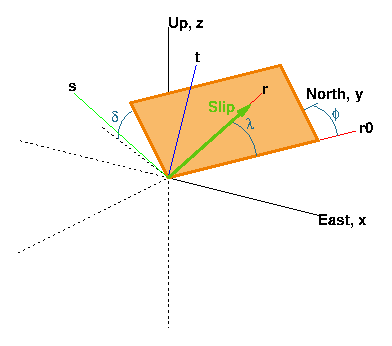
\includegraphics{boundaryconditions/figs/faultOrientation}
  \caption{Orientation of a fault surface in 3D, where $\phi$ denotes the angle
    of the fault strike, $\delta$ denotes the angle of the fault dip,
    and $\lambda$ the rake angle.}
  \label{fig:fault:orientation} 
\end{figure}

\begin{figure}[htbp]
  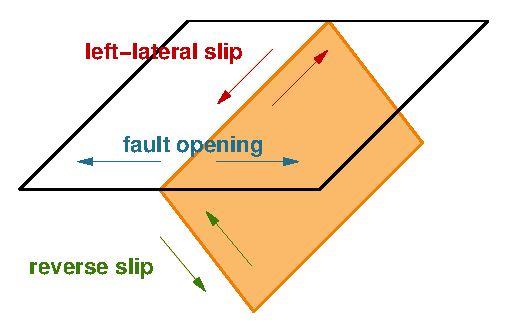
\includegraphics{boundaryconditions/figs/slipmotions}
  \caption{Sign conventions associated with fault slip. Positive values are associated
    with left-lateral, reverse, and fault opening motions.}
  \label{fig:fault:slip:motions} 
\end{figure}

\subsection{Fault Implementation}

In order to create relative motion across the fault surface in the
finite-element mesh, additional degrees of freedom are added along
with adjustment of the topology of the mesh. These additional degrees
of freedom are associated with cohesive cells. These zero-volume cells
allow control of the relative motion between vertices on the two sides
of the fault. PyLith automatically adds cohesive cells for each fault
surface. Figure \vref{fig:fault:cohesive:cells} illustrates the results
of inserting cohesive cells in a mesh consisting of triangular cells.
This example also shows the distinction between how buried fault edges
are handled differently than fault edges that reach the edge of the
domain, such as the ground surface.

\begin{figure}[htbp]
  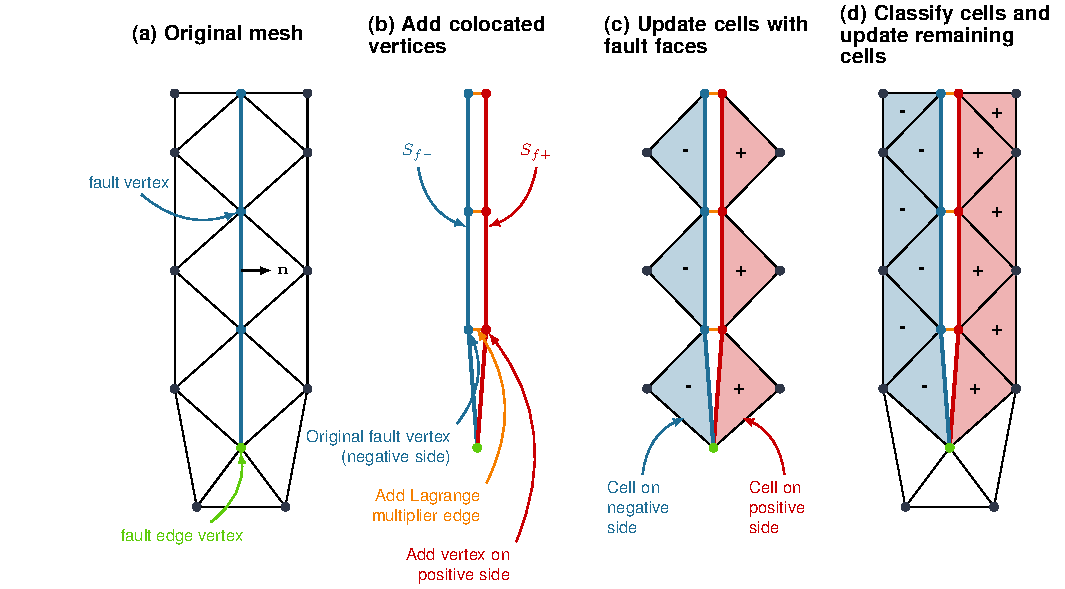
\includegraphics[width=6.25in]{boundaryconditions/figs/cohesivecell}
  \caption{Example of cohesive cells inserted into a mesh of
    triangular cells.  The zero thickness cohesive cells control slip
    on the fault via the relative motion between the vertices on the
    positive and negative sides of the fault.}
  \label{fig:fault:cohesive:cells} 
\end{figure}

\begin{figure}[htbp]
  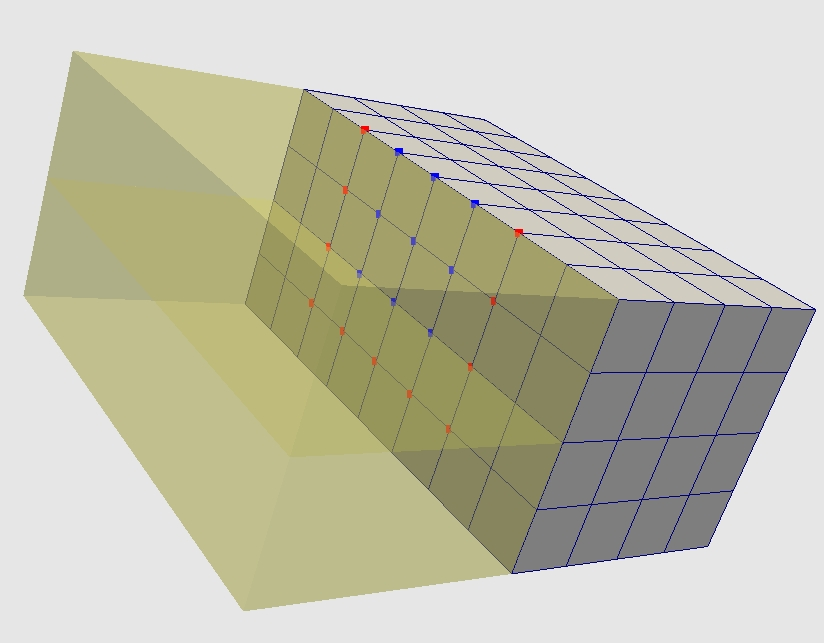
\includegraphics[width=4in]{boundaryconditions/figs/faultEdge}
  \caption{Example of how faults with buried edges must be described
    with two sets of vertices. All of the vertices on the fault are
    included in the \texttt{fault} group; the subset of vertices along
    the buried edges are included in the \texttt{fault\_edge}
    group. In 2-D the fault edges are just a single vertex as shown in
    Figure
    \vref{fig:fault:cohesive:cells}(a).}
  \label{fig:fault:fault_edge}
\end{figure}
For faults that have buried edges, splitting the mesh apart and inserting
the cohesive cells becomes complex at the buried edges due to the
ambiguity of defining where the fault ends and how to insert the cohesive
cell. In PyLith v2.0.0 we have changed how the buried edges of the
fault are managed. An additional group of fault nodes is specified
(e.g., via a nodeset from CUBIT) that marks the buried edges of the
fault (see Figure \vref{fig:fault:fault_edge}). This allows the cohesive
cell insertion algorithm to adjust the topology so that cohseive cells
are inserted up to the buried edge of the fault but no additional
degrees of freedom are added on the fault edge. This naturally forces
slip to zero along the buried edges.

\subsection{Fault Parameters}

The principal parameters for fault interface conditions are:
\begin{inventory}
\propertyitem{id}{This is an integer identifier for the fault surface. It is
used to specify the \property{material-id} of the cohesive cells in
the mesh. Material identifiers must be unique so this value cannot
be the same as any of the material models or any other fault.}
\propertyitem{label}{Name of group of vertices associated with the fault surface.
This label is also used in error and diagnostic reports.}
\propertyitem{edge}{Name of group of vertices marking the buried edges of the
fault.}
\propertyitem{up\_dir}{Up-dir or up direction (used in 2D and 3D simulations).
In 2D the default in-plane slip is left-lateral, so we use the up-direction
to resolve the ambiguity in specifying reverse slip. In 3D the up-direction
is used to resolve the ambiguity in the along-strike and dip-dir directions.
If the fault plane is horizontal, then the up-dir corresponds to the
reverse-motion on the +z side of the fault. The only requirement for
this direction is that it not be collinear with the fault normal direction.
The default value of [0, 0, 1] is appropriate for most 3D problems.}
\facilityitem{quadrature}{Quadrature object used in integrating fault quantities.}
\facilityitem{output}{Manager for output of diagnostic and data fields for the fault.}
\end{inventory}
By default the output manager outputs both diagnostic information
(e.g., fault normal direction) and the slip at each time step. Tables
\vref{tab:fault:kin:output} and \vref{tab:fault:dyn:output} list the
fields available for output for a fault with kinematic (prescribed)
earthquake rupture and a fault with dynamic rupture, respectively.
The fault coordinate system is shown in Figure \vref{fig:fault:slip:motions}.
The vectors in the fault coordinate system can be transformed to the
global coordinate system using the direction vectors in the diagnostic
output. An example of setting these parameters in a \filename{.cfg}
file is:
\begin{cfg}
<h?[pylithapp.problem]</h>
<p>interfaces</p> = [fault] 

<h>[pylithapp.problem.interfaces]</h>
<f>fault</f> = pylith.faults.FaultCohesiveKin ; default
<p>label</p> = fault_A ; Group of vertices defining the fault surface
<p>edge</p> = fault_edge ; Group of vertices defining the buried edges
<p>id</p> = 100 ; Value for material identifier associated with fault's cohesive cells
<p>up_dir</p> = [0, 0, 1] ; default
<f>quadrature.cell</f> = pylith.feassemble.FIATLagrange
<p>quadrature.cell.dimension</p> = 2
\end{cfg}
The group of vertices has the label ``fault A.'' We replicate the
default values for the fault ``up'' direction. These settings apply
to a 2D fault surface embedded within a 3D mesh, so we use 2D Lagrange
reference cells. The spatial database for elastic properties is used
to determine the approximate shear modulus and condition the equations
for faster convergence rates.


\subsection{Kinematic Earthquake Rupture}

Kinematic earthquake ruptures use the FaultCohesiveKin object to specify
the slip as a function of time on the fault surface. Slip may evolve
simultaneously over the fault surface instantaneously in a single
time step (as is usually done in quasi-static simulations) or propagate
over the fault surface over hundreds and up to thousands of time steps
(as is usually done in a dynamic simulation).


\subsubsection{Governing Equations}

The insertion of cohesive cells into the finite-element mesh has the
effect of decoupling the motion of the two sides of the fault surface.
In order to impose the desired relative motion, we must adjust the
governing equations. PyLith employs Lagrange multiplier constraints
to enforce the constraint of the relative motion in the strong sense.
That is, we enforce the slip across the fault at each degree of freedom.

In conventional implementations the additional degrees of freedom
associated with the Lagrange multipliers result in a complex implementation.
However, the use of Lagrange multiplier constraints with cohesive
cells provides for a simple formulation; we simply add the additional
degrees of freedom associated with the Lagrange multipliers to the
cohesive cells as shown in Figure \vref{fig:fault:cohesive:cells}.
As a result, the fault implementation is completely confined to the
cohesive cell. Furthermore, the Lagrange multiplier constraints correspond
to forces required to impose the relative motions, so they are related
to the change in stress on the fault surface associated with fault
slip. If we write the algebraic system of equations associated with
elasticity in the form
\begin{equation}
\underline{A}\overrightarrow{u}=\overrightarrow{b}\,,
\end{equation}
then adding in the Lagrange multiplier constraints associated with
fault slip leads to a new system of equations of the form 
\begin{equation}
\left[\begin{array}{cc}
\underline{A} & \underline{C}^{T}\\
\underline{C} & 0
\end{array}\right]\left[\begin{array}{c}
\overrightarrow{u}\\
\overrightarrow{l}
\end{array}\right]=\left[\begin{array}{c}
\overrightarrow{b}\\
\overrightarrow{d}
\end{array}\right]\,,\label{eq:fault:cohesive:lagrange}
\end{equation}
where $\overrightarrow{l}$ is the vector of Lagrange multipliers
and $\underline{C}$ is composed of rotation submatrices, $\underline{R}$,
associated with the direction cosines relating the relative displacements
across the fault to the vector of fault slip, $\overrightarrow{d}$.
Note that by using the direction cosines to relate the relative motion
across the fault, the slip vector and Lagrange multipliers (forces
required to impose the slip) are in the local fault coordinate system
(lateral motion, reverse motion, and fault opening). 

\paragraph{Non-diagonal A}

The Lagrange multipliers contribute to both the system Jacobian matrix
and the residual. Because we enforce the constraints in a strong sense,
the terms do not involve integrals over the fault surface. The additional
terms in the residual are
\begin{gather}
r_{i}^{n}=-C_{ji}^{pn}l_{j}^{p},\\
r_{i}^{p}=d_{i}^{p}-C_{ij}^{pn}u_{j}^{n},
\end{gather}
where $n$ denotes a conventional degree of freedom and $p$ denotes
a degree of freedom associated with a Lagrange multiplier. The additional
terms in the system Jacobian matrix are simply the direction cosines,
\begin{gather}
J_{ij}^{np}=C_{ji}^{pn},\\
J_{ij}^{pn}=C_{ij}^{pn}.
\end{gather}

\paragraph{Diagonal A}

When we use a lumped system Jacobian matrix, we cannot lump the terms
associated with the Lagrange multipliers. Instead, we formulate the
Jacobian ignoring the contributions from the Lagrange multipliers,
and then adjust the solution after the solve to account for their
presence. Including the Lagrange multipliers in the general expression
for the residual at time $t+\Delta t$, we have
\begin{equation}
r_{i}^{n}(t+\Delta t)=A_{ij}^{nm}(u_{j}^{m}(t)+du_{j}^{m}(t))+C_{ki}^{pn}(l_{k}^{p}(t)+dl_{k}^{p}(t)),
\end{equation}
where we have written the displacements and Lagrange multipliers at
time $t+\Delta t$ in terms of the values at time $t$ and the increment
from time $t$ to $t+\Delta t$. When we solve the lumped system ignoring
the Lagrange multipliers contributions to the Jacobian, we formulate
the residual assuming the values $du_{i}^{n}$(t) and $dl_{k}^{p}(t)$
are zero. So our task is to determine the increment in the Lagrange
multiplier, $dl_{k}^{p}$, and the correction to the displacement
increment, $du_{i}^{n}$, and by setting the residual with all terms
included to zero; thus, we have
\begin{gather}
A_{ij}^{nm}(u_{j}^{m}(t)+du_{j}^{m}(t))+C_{ki}^{pn}(l_{k}^{p}(t)+dl_{k}^{p}(t))=0\text{ subject to}\\
C_{ij}^{pn}(u_{j}^{n}(t)+du_{j}^{n}(t))=d_{i}^{p}.
\end{gather}
Making use of the residual computed with $du_{i}^{n}(t)=0$ and $dl_{k}^{p}(t)=0$,
\begin{gather}
r_{i}^{n}+A_{ij}^{nm}du_{j}^{m}+C_{ki}^{pn}dl_{k}^{p}=0\text{ subject to}\\
C_{ij}^{pn}(u_{j}^{n}(t)+du_{j}^{n}(t))=d_{i}^{p}.
\end{gather}
Explicitly writing the equations for the vertices on the negative
and positive sides of the fault yields
\begin{gather}
r_{i}^{n-}+A_{ij}^{nm-}du_{j}^{m-}+R_{ki}^{pn}dl_{k}^{p}=0,\\
r_{i}^{n+}+A_{ij}^{nm+}du_{j}^{m+}+R_{ki}^{pn}dl_{k}^{p}=0,\\
R_{ij}^{pn}(u_{j}^{n+}+du_{j}^{n+}-u_{j}^{n-}-du_{j}^{n-})=d_{i}^{p}.
\end{gather}
Solving the first two equations for $du_{j}^{m-}$ and $du_{j}^{m+}$
and combining them using the third equation leads to
\begin{multline}
R_{ij}^{pn}\left((A_{ij}^{nm+})^{-1}+(A_{ij}^{nm+})^{-1}\right)R_{ki}^{pn}dl_{k}^{p}=d_{i}^{p}-R_{ij}^{pn}(u_{j}^{n+}-u_{j}^{n-})\\
+R_{ij}^{pn}\left((A_{ij}^{nm+})^{-1}r_{i}^{n+}-(A_{ij}^{nm-})^{-1}r_{i}^{n-}\right).
\end{multline}
We do not allow overlap between the fault interface and the absorbing
boundary, so $A_{ij}^{nm}$ is the same for all components at a vertex.
As a result the matrix on the left hand side simplifies to
\begin{equation}
S_{ik}^{pn}=\delta_{ik}\left(\frac{1}{A^{nm+}}+\frac{1}{A^{nm-}}\right),
\end{equation}
and
\begin{equation}
dl_{k}^{p}=(S_{ik}^{pn})^{-1}\left(d_{i}^{p}-R_{ij}^{pn}(u_{j}^{n+}-u_{j}^{n-})+R_{ij}^{pn}\left((A_{ij}^{nm+})^{-1}r_{i}^{n+}-(A_{ij}^{nm-})^{-1}r_{i}^{n-}\right)\right).
\end{equation}
Now that we know the value of the increment in the Lagrange multiplier
from time $t$ to time $t+\Delta t$, we can correct the value for
the displacement increment from time $t$ to $t+\Delta t$ using
\begin{gather}
\Delta du_{j}^{n-}=(A_{ij}^{nm-})^{-1}C_{ki}^{pn}dl_{k}^{p}\text{ and}\\
\Delta du_{j}^{n+}=-(A_{ij}^{nm+})^{-1}C_{ki}^{pn}dl_{k}^{p}.
\end{gather}

\subsubsection{Arrays of Kinematic Rupture Components}

Multiple earthquake ruptures can be specified on a single fault surface.
This permits repeatedly rupturing the same portion of a fault or combining
earthquake rupture on one subset of the fault surface with steady
aseismic slip on another subset (the two subsets may overlap in both
time and space). A dynamic array of kinematic earthquake rupture components
associates a name (string) with each kinematic rupture. The default
dynamic array contains a single earthquake rupture, ``rupture''. The
\property{eq\_srcs} is the \object{FaultCohesiveKin} facility for this
dynamic array. An example of setting the array of kinematic rupture
components in a \filename{.cfg} file:
\begin{cfg}
<h<[pylithapp.problem.interfaces.fault]</h>
<p>eq_srcs</p> = [earthquake,creep]
\end{cfg}
The output manager includes generic fault information (orientation)
as well as the final slip or slip rate (as in the case of the constant
slip rate slip time function) and slip initiation time for each kinematic
rupture. The name of the slip and slip initiation time vertex fields
are of the form \texttt{final\_slip\_NAME} and \texttt{slip\_time\_NAME},
respectively, where \texttt{NAME} refers to the name used in the dynamic
array of kinematic ruptures, \property{eq\_srcs}.

\begin{table}[htbp]
\caption{Fields available in output of fault information.}
\label{tab:fault:kin:output}
\begin{tabular}{llp{3.5in}}
\textbf{Field Type} & \textbf{Field} & \textbf{Description}\\
\hline 
\property{vertex\_info\_fields} & \texttt{normal\_dir} & Direction of fault normal in global coordinate system\\
 & \texttt{strike\_dir} & Direction of fault strike in global coordinate system\\
 & \texttt{dip\_dir} & Up-dip direction on hanging wall in global coordinate system\\
 & \texttt{final\_slip\_NAME} & Vector of final slip (in fault coordinate system) in meters\\
 & \texttt{slip\_time}\_\texttt{\noun{NAME}} & Time at which slip begins in seconds\\
\property{vertex\_data\_fields} & \texttt{slip} & Slip vector at time step (in fault coordinate system) in meters\\
 & \texttt{traction\_change} & Change in fault tractions (in fault coordinate system) in Pa\\
\hline 
\end{tabular}
\end{table}


\subsubsection{Kinematic Rupture Parameters}

The kinematic rupture parameters include the origin time and slip
time function. The slip initiation time in the slip time function
is relative to the origin time (default is 0). This means that slip
initiates at a point at a time corresponding to the sum of the kinematic
rupture's origin time and the slip initiation time for that point.
An example of specifying the kinematic earthquake rupture properties
and components in a \filename{.cfg} file:
\begin{cfg}
<h>[pylithapp.problem.interfaces.fault]</h>

<p>eq_srcs</p> = [earthquake,creep]

<h>[pylithapp.problem.interfaces.fault.eq_srcs.earthquake]</h>
<p>origin_time</p> = 0.0*s ; default origin time
<f>slip_function</f> = pylith.faults.StepSlipFn ; default slip time function

<h>[pylithapp.problem.interfaces.fault.eq_srcs.creep]</h>
<p>origin_time</p> = 10.0*year ; start creep at 10.0 years

<f>slip_function</f> = pylith.faults.ConstRateSlipFn ; switch to constant slip rate slip function
\end{cfg}

\subsubsection{Slip Time Function}

The current release of PyLith supports specification of the evolution
of fault slip using analytical expressions for the slip time history
at each point, where the parameters for the slip time function may
vary over the fault surface. Currently, three slip time functions
are available: (1) a step-function for quasi-static modeling of earthquake
rupture, (2) a constant slip rate time function for modeling steady
aseismic slip, and (3) the integral of Brune's far-field time function
\cite{Brune:1970} for modeling the dynamics of earthquake rupture.
Additional slip time functions will likely be available in future
releases. The default slip time function is the step-function slip
function.


\paragraph{Step-Function Slip Time Function}

This slip function prescribes a step in slip at a given time at a
point: 
\begin{gather}
D(t)=\left\{ \begin{array}{cc}
0 & 0\leq t<t_{r}\\
D_{final} & t\ge t_{r}
\end{array}\right.\,,
\end{gather}
where $D(t)$ is slip at time $t$, $D_{final}$ is the final slip,
and $t_{r}$ is the slip initiation time (time when rupture reaches
the location). The slip is specified independently for each of the
components of slip, and the slip and slip starting time may vary over
the fault surface.
\begin{inventory}
\facilityitem{final\_slip}{Spatial database of slip ($D_{final})$.}
\facilityitem{slip\_time}{Spatial database of slip initiation times ($t_{r}$).}
\end{inventory}
An example of setting these parameters in a \filename{.cfg} file is:
\begin{cfg}
<h>[pylithapp.problem.interfaces.fault.eq_srcs.rupture]</h>
<f>slip_function</f> = pylith.faults.StepSlipFn 

<h>[pylithapp.problem.interfaces.fault.eq_srcs.rupture.slip_function]</h>
<p>final_slip.iohandler.filename</p> = final_slip.spatialdb
<p>slip_time.iohandler.filename</p> = sliptime.spatialdb
\end{cfg}
The spatial database files for the slip time function specify the
spatial variation in the parameters for the slip time function, as
shown in Table \vref{tab:slip:function:step}.

\begin{table}[htbp]
  \caption{Values in spatial database used as parameters in the step function slip time function.}
  \label{tab:slip:function:step}
  \begin{tabular}{llp{2.5in}}
    \textbf{Spatial database} & \textbf{Value} & \textbf{Description}\\
    \hline 
    \facility{final\_slip} & \texttt{left-lateral-slip} & Amount of left-lateral final slip in meters. Use negative values for right-lateral slip. \\
      & \texttt{reverse-slip} & Amount of reverse slip in meters. Use negative values for normal slip. \\
      & \texttt{fault-opening} & Amount of fault opening in meters. Negative values imply penetration.\\
\facility{slip\_time} & \texttt{slip-time} & Slip initiation time ($t_{t})$ in seconds.\\
    \hline 
  \end{tabular}
\end{table}


\paragraph{Constant Slip Rate Slip Time Function}

This slip function prescribes a constant slip rate for the evolution
of slip at a point: 
\begin{gather}
  D(t)=\left\{ \begin{array}{cc}
0 & 0\leq t<t_{r}\\
V(t-t_{r}) & t\ge t_{r}
\end{array}\right.\,,
\end{gather}
where $D(t)$ is slip at time $t$, $V$ is the slip rate, and $t_{r}$
is the slip initiation time (time when rupture reaches the location).
The slip rate is specified independently for each of the components
of slip, and the slip rate and slip starting time may vary over the
fault surface.
\begin{inventory}
\facilityitem{slip\_rate}{Spatial database of slip rate ($V$).}
\facilityitem{slip\_time}{Spatial database of slip initiation times ($t_{r}$).}
\end{inventory}
An example of setting these parameters in a \filename{.cfg} file is:
\begin{cfg}
<h>[pylithapp.problem.interfaces.fault.eq_srcs.ruptures]</h>
<f>slip_function</f> = pylith.faults.ConstRateSlipFn 

<h>[pylithapp.problem.interfaces.fault.eq_srcs.ruptures.slip_function]</h>
<p>slip_rate.iohandler.filename</p> = slip_rate.spatialdb
<p>slip_time.iohandler.filename</p> = sliptime.spatialdb
\end{cfg}
The spatial database files for the slip time function specify the
spatial variation in the parameters for the slip time function, as
shown in Table \vref{tab:slip:function:constant:rate}.

\begin{table}[htbp]
\caption{Values in spatial database used as parameters in the constant slip rate slip time function.}
\label{tab:slip:function:constant:rate}
\begin{tabular}{llp{2.5in}}
\textbf{Spatial database} & \textbf{Value} & \textbf{Description}\\
\hline 
\facility{slip\_rate} & \texttt{left-lateral-slip} & Slip rate for left-lateral final slip in meters per second. Use negative
values for right-lateral slip. \\
 & \texttt{reverse-slip} & Slip rate for reverse slip in meters per second. Use negative values
for normal slip. \\
 & \texttt{fault-opening} & Slip rate for fault opening in meters per second. Negative values
imply penetration.\\
\facility{slip\_time} & \texttt{slip-time} & Slip initiation time ($t_{t})$ in seconds.\\
\hline 
\end{tabular}
\end{table}

\paragraph{Brune Slip Time Function}

We use an integral of Brune's far-field time function \cite{Brune:1970}
to describe the evolution in time of slip at a point: 
\begin{gather}
D(t)=\left\{ \begin{array}{cc}
0 & 0\leq t<t_{r}\\
D_{final}\left(1-exp\left(-\frac{t-t_{r}}{t_{0}}\right)\left(1+\frac{t-t_{r}}{t_{0}}\right)\right) & t\ge t_{r}
\end{array}\right.\,,\\
t_{0}=0.6195t_{\mathit{rise}}\,,
\end{gather}
where $D(t)$ is slip at time $t$, $D_{final}$ is the final slip
at the location, $t_{r}$ is the slip initiation time (time when rupture
reaches the location), and $t_{\mathit{rise}}$ is the rise time.
\begin{inventory}
\facilityitem{slip}{Spatial database of final slip distribution ($D_{final})$.}
\facilityitem{slip\_time}{Spatial database of slip initiation times ($t_{r}$).}
\facilityitem{rise\_time}{Spatial database for rise time ($t_{\mathit{rise}}$).}
\end{inventory}
An example of setting these parameters in a \filename{.cfg} file is:
\begin{cfg}
<h>[pylithapp.problem.interfaces.fault.eq_srcs.ruptures]</h>
<f>slip_function</f> = pylith.faults.BruneSlipFn

<h>[pylithapp.problem.interfaces.fault.eq_srcs.rupture.slip_function]</h>
<p>slip.iohandler.filename</p> = finalslip.spatialdb
<p>rise_time.iohandler.filename</p> = risetime.spatialdb
<p>slip_time.iohandler.filename</p> = sliptime.spatialdb
\end{cfg}
The spatial database files for the slip time function specify the
spatial variation in the parameters for the slip time function, as
shown in Table \vref{tab:slip:function:Brune}.

\begin{table}[htbp]
\caption{Values in spatial database used as parameters in the Brune slip time function.}
\label{tab:slip:function:Brune}
\begin{tabular}{llp{2.5in}|}
\textbf{Spatial database} & \textbf{Value} & \textbf{Description}\\
\hline 
\facility{slip} & \texttt{left-lateral-slip} & Amount of left-lateral final slip in meters. Use negative values for right-lateral slip. \\
 & \texttt{reverse-slip} & Amount of reverse slip in meters. Use negative values for normal slip.
\\
 & \texttt{fault-opening} & Amount of fault opening in meters. Negative values imply penetration.\\
\facility{rise\_time} & \texttt{rise-time} & Rise time ($t_{r})$ in seconds.\\
\facility{slip\_time} & \texttt{slip-time} & Slip initiation time ($t_{t})$ in meters.\\
\hline 
\end{tabular}
\end{table}


\paragraph{Liu-Cosine Slip Time Function}

This slip time function, proposed by Liu, Archuleta, and Hartzell
for use in ground-motion modeling\cite{Liu:etal:2006}, combines several
cosine and sine functions together to create a slip time history with
a sharp rise and gradual termination with a finite duration of slip.
The evolution of slip at a point follows: 
\begin{gather}
D(t)=\left\{ \begin{array}{cc}
D_{\mathit{final}}C_{n}\left(0.7t-0.7\frac{t_{1}}{\pi}\sin\frac{\pi t}{t_{1}}-1.2\frac{t_{1}}{\pi}\left(\cos\frac{\pi t}{2t_{1}}-1\right)\right) & 0\leq t<t_{1}\\
D_{\mathit{final}}C_{n}\left(1.0t-0.7\frac{t1}{\pi}\sin\frac{\pi t}{t_{1}}+0.3\frac{t2}{\pi}\sin\frac{\pi(t-t1)}{t_{2}}+\frac{1.2}{\pi}t_{1}-0.3t_{1}\right) & t_{1}\leq t<2t_{1}\\
D_{\mathit{final}}C_{n}\left(0.7-0.7\cos\frac{\pi t}{t_{1}}+0.6\sin\frac{\pi t}{2t_{1}}\right) & 2t_{1}\leq t\leq t_{0}
\end{array}\right.\,,\\
C_{n}=\frac{\pi}{1.4\pi t_{1}+1.2t_{1}+0.3\pi t_{2}},\\
t_{0}=1.525t_{\mathit{rise}},\\
t_{1}=0.13t_{0},\\
t_{2}=t_{0}-t_{1},
\end{gather}
where $D(t)$ is slip at time $t$, $D_{final}$ is the final slip
at the location, $t_{r}$ is the slip initiation time (time when rupture
reaches the location), and $t_{\mathit{rise}}$ is the rise time.
\begin{inventory}
\facilityitem{slip}{Spatial database of final slip distribution ($D_{final})$.}
\facilityitem{slip\_time}{Spatial database of slip initiation times ($t_{r}$).}
\facilityitem{rise\_time}{Spatial database for rise time ($t_{\mathit{rise}}$).}
\end{inventory}
The spatial database files for the slip time function use the same
parameters for the slip time function as the Brune slip time function
shown in Table \vref{tab:slip:function:Brune}.


\paragraph{Time-History Slip Time Function}

This slip time function reads the slip time function from a data file,
so it can have an arbitrary shape. The slip and slip initiation times
are specified using spatial databases, so the slip time function,
in general, will use a normalized amplitude.
\begin{inventory}
\facilityitem{slip}{Spatial database of final slip distribution ($D_{final})$.}
\facilityitem{slip\_time}{Spatial database of slip initiation times ($t_{r}$).}
\facilityitem{time\_history}{Temporal database for slip evolution.}
\end{inventory}
An example of setting these parameters in a \filename{.cfg} file is:
\begin{cfg}
<h>[pylithapp.problem.interfaces.fault.eq_srcs.ruptures]</h>
<f>slip_function</f> = pylith.faults.TimeHistorySlipFn 

<h>[pylithapp.problem.interfaces.fault.eq_srcs.rupture.slip_function]</h>
<p>slip.iohandler.filename</p> = finalslip.spatialdb
<p>slip_time.iohandler.filename</p> = sliptime.spatialdb
<p>time_history.iohandler.filename</p> = myfunction.timedb
\end{cfg}
The spatial database files for the slip time function specify the
spatial variation in the parameters for the slip time function, as
shown in Table \vref{tab:slip:function:Brune-2}.

\begin{table}[htbp]
\caption{Values in spatial database used
as parameters in the time history slip time function.}
\label{tab:slip:function:Brune-2}
\begin{tabular}{llp{2.5in}}
\textbf{Spatial database} & \textbf{Value} & \textbf{Description}\\
\hline 
\facility{slip} & \texttt{left-lateral-slip} & Amount of left-lateral final slip in meters. Use negative values for
right-lateral slip. \\
 & \texttt{reverse-slip} & Amount of reverse slip in meters. Use negative values for normal slip.
\\
 & \texttt{fault-opening} & Amount of fault opening in meters. Negative values imply penetration.\\
\facility{rise\_time} & \texttt{rise-time} & Rise time ($t_{r})$ in seconds.\\
\facility{slip\_time} & \texttt{slip-time} & Slip initiation time ($t_{t})$ in meters.\\
\hline 
\end{tabular}
\end{table}


\subsection{Dynamic Earthquake Rupture}

Dynamic fault interfaces use the FaultCohesiveDyn object to specify
a fault constitutive model to govern the fault tractions (friction)
and the resulting slip. When friction is large enough such that there
is no sliding on the fault, the fault is locked (slip is zero) and
the Lagrange multipliers assume their values just as they do in kinematic
ruptures. In this case, the Lagrange multipliers correspond to the
forces necessary to keep the slip zero. When the driving forces exceed
those allowed by friction, we reduce the values of the Lagrange multipliers
to those consistent with friction from the fault constitutive model.
When we reduce the Lagrange multipliers, we must increment the slip
accordingly to maintain consistency in the algebraic system of equations.


\subsubsection{Governing Equations}

The algebraic systems of equations for dynamic earthquake rupture
are the same as those for kinematic rupture
\begin{equation}
\left[\begin{array}{cc}
\underline{A} & \underline{C}^{T}\\
\underline{C} & 0
\end{array}\right]\left[\begin{array}{c}
\overrightarrow{u}\\
\overrightarrow{l}
\end{array}\right]=\left[\begin{array}{c}
\overrightarrow{b}\\
\overrightarrow{d}
\end{array}\right].
\end{equation}
Enforcing the limits imposed on the Lagrange multipliers by the fault
constitutive model requires determining the increment in slip for
an increment in the Lagrange multipliers. The increment in the Lagrange
multipliers is the difference between the value computed for the current
slip (either zero or the slip at the previous time step) and the value
computed from the fault constitutive model. Starting from our system
of algebraic equations,
\begin{equation}
A_{ij}^{nm}u_{j}^{m}+C_{ji}^{pn}l_{j}^{p}=b_{i}^{n},
\end{equation}
we compute the sensitivity for the given loading and boundary conditions,
\begin{equation}
A_{ij}^{nm}\partial u_{j}^{m}=-C_{ji}^{pn}\partial l_{j}^{p}.
\end{equation}
Computing the increment in the slip requires computing the increment
in the displacements. Solving this equation rigorously would require
inverting the system Jacobian, which we do not want to do unless it
is diagonal (as it is in the case of the lumped formulations). 


\paragraph{Non-Diagonal A}

In general A is a sparse matrix with off-diagonal terms of the form
\begin{equation}
A=\left(\begin{array}{ccc}
A_{0} & A_{1} & A_{2}\\
A_{3} & A_{n-} & 0\\
A_{4} & 0 & A_{n+}
\end{array}\right),
\end{equation}
where the degrees of freedom on either side of the fault are uncoupled.
We formulate two small linear systems involving just the degrees of
freedom associated with vertices on either the positive or negative
sides of the fault,
\begin{gather}
A_{ij}^{nm-}\partial u_{j}^{m-}=-R_{ij}^{pn}\partial l_{j}^{p},\\
A_{ij}^{nm+}\partial u_{j}^{m+}=R_{ij}^{pn}\partial l_{j}^{p},
\end{gather}
where we have replaced $\underline{C}$ with $\underline{R}$ to denote
the explicit inclusion of the signs for the terms in $\underline{C}$
associated with the positive ($n^{+}$) and negative ($n^{-}$) sides
of the fault. After solving these two linear systems of equations,
we compute the increment in slip using
\begin{equation}
\partial d_{i}^{p}=R_{ij}^{pn}(\partial u_{j}^{n+}-\partial u_{j}^{n-}).
\end{equation}
The solution of these two linear systems gives the increment in slip
assuming all the degrees of freedom except those immediately adjacent
to the fault remain fixed. In real applications where the deformation
associated with fault slip is localized around the fault, this provides
good enough approximations so that the nonlinear solver converges
quickly. In problems where deformation associated with slip on the
fault is not localized (as in the case in some of the example problems),
the increment in slip computed by solving these two linear systems
is not a good approximation and the nonlinear solve requires a large
number of iterations.

We use the PETSc Krylov subspace solver (KSP) to solve these two linear
systems. The PETSc settings for the KSP object are set in the same
manner as the main solver, except we use the pvrefix \texttt{friction\_}
in all of the settings related to the KSP solver for these two linear
systems. For example, to use the recommended additive Schwarz preconditioner
in the friction sensitivity solves, the settings in a \texttt{.cfg}
file are:
\begin{cfg}
<h>[pylithapp.petsc]</h>
<p>friction_pc_type</p> = asm
\end{cfg}
See the examples in Sections \vref{sec:example:3dhex8:friction}
and \vref{sec:example:shearwave:quad4} for details.


\paragraph{Diagonal A}

With a lumped Jacobian matrix, we can solve for the increment in slip
directly,
\begin{equation}
\partial d_{i}^{p}=-C_{ij}^{pn}(A_{jk}^{nm})^{-1}C_{lk}^{pm}\partial l_{l}^{p}.
\end{equation}
By not allowing the fault interface to overlap with the absorbing
boundary, the terms in $A$ for a given vertex are identical and the
expression on the right-hand side reduces to
\begin{equation}
\partial d_{i}^{p}=-\left(\frac{1}{A^{n+}}+\frac{1}{A^{n-}}\right)\partial l_{i}^{p}.
\end{equation}

\subsubsection{Dynamic Rupture Parameters}

The properties and facilities of the \object{FaultCohesiveDyn} object include
\begin{inventory}
\propertyitem{open\_free\_surface}{If true, enforce traction free surface when
the fault opens, otherwise apply prescribed tractions even when the
fault opens (default is true); to mimic a dike opening, use false.}
\propertyitem{zero\_tolerance}{Tolerance for detecting zero values (default
is 1.0e-10); should be larger than absolute tolerance in KSP solves.}
\facilityitem{traction\_perturbation}{Prescribed tractions on fault surface
(generally used for nucleating earthquake ruptures; default is none).}
\facilityitem{friction}{Fault constitutive model.}
\end{inventory}
An example of specifying the dynamic earthquake rupture properties
and components in a \filename{.cfg} file:
\begin{cfg}
<h>[pylithapp.problem.interfaces.fault]</h>
<p>open_free_surface</p> = True ; default

<f>traction_perturbation</f> = pylith.faults.TractPerturbation ; not default
<f>traction_perturbation.db_initial</f> = spatialdata.spatialdb.SimpleDB
<p>traction_perturbation.db_initial.iohandler.filename</p> = tractions.spatialdb

<f>friction<f> = pylith.friction.StaticFriction
<f>friction.db_properties</f> = spatialdata.spatialdb.SimpleDB
<p>friction.db_properties.iohandler.filename</p> = friction.spatialdb
\end{cfg}

\warning{Use of the dynamic rupture implementation in a quasi-static
  simulations requires use of the nonlinear solver.}

\important{The dynamic rupture implementation requires careful
  selection of linear and nonlinear solver tolerances.  A key issue is
  making sure the linear solver toleance is tighter (smaller) than the
  tolerance used to detect slip (fault \property{zero\_toelerance}).
  As a result, the linear and solver absolute tolerances should be
  used to for convergence, not the relative tolerances. The settings below
  illustrates the relevant parameters and example values. The values
  can be scaled to change the overall desired tolerances.}

\begin{cfg}
<h>[pylithapp.problem.interfaces.fault]</h>
<p>zero_tolerance</p> = 1.0e-11

<h>[pylithapp.petsc]</h>
# Linear solver tolerances
<p>ksp_rtol</p> = 1.0e-20
<p>ksp_atol</p> = 1.0e-12

# Nonlinear solver tolerances
<p>snes_rtol</p> = 1.0e-20
<p>snes_atol</p> = 1.0e-10

# Set preconditioner for friction sensitivity solve
<p>friction_pc_type</p> = asm
<p>friction_sub_pc_factor_shift_type<p> = nonzero
\end{cfg}

The prescribed traction perturbation is specified using the same fault
coordinate system as the slip directions in the kinematic ruptures.
The perurbation has the same functional form as the time-dependent
boundary conditions (and same spatial databases). Table
\vref{tab:fault:cohesive:dyn:prescribed:tractions} gives the values in
the spatial database for the prescribed tractions.  Table
\vref{tab:fault:dyn:output} shows the fields available for output.
Additional fields are available depending on the fault constitutive
model.

\begin{table}[htbp]
\caption{Values in spatial databases for prescribed tractions.}
\label{tab:fault:cohesive:dyn:prescribed:tractions}
\begin{tabular}{lllp{2.5in}}
\textbf{Spatial database} & \textbf{Dimension} & \textbf{Value} & \textbf{Description}\\
\hline 
\facility{db\_initial} & 2D & \texttt{traction-shear} & Left-lateral shear traction (reverse shear for dipping faults)\\
 &  & \texttt{traction-normal} & Normal traction (tension is positive)\\
 & 3D & \texttt{traction-shear-leftlateral} & Left-lateral shear traction\\
 &  & \texttt{traction-shear-updip} & Reverse shear traction\\
 &  & \texttt{traction-normal} & Normal traction (tension is positive)\\
\facility{db\_rate} & 2D & \texttt{traction-rate-shear} & Rate of change of left-lateral shear traction (reverse shear for dipping
faults)\\
 &  & \texttt{traction-rate-normal} & Rate of change of normal traction (tension is positive)\\
 & 3D & \texttt{traction-rate-leftlateral} & Rate of change of left-lateral shear traction\\
 &  & \texttt{traction-rate-shear-updip} & Rate of change of reverse shear traction\\
 &  & \texttt{traction-rate-normal} & Rate of change of normal traction (tension is positive)\\
 & all & \texttt{rate-start-time} & Time at which rate of change begins\\
\facility{db\_change} & 2D & \texttt{traction-shear} & Change in left-lateral shear traction (reverse shear for dipping faults)\\
 &  & \texttt{traction-normal} & Change in normal traction (tension is positive)\\
 & 3D & \texttt{traction-leftlateral} & Change in left-lateral shear traction\\
 &  & \texttt{traction-shear-updip} & Change in reverse shear traction\\
 &  & \texttt{traction-normal} & Change in normal traction (tension is positive)\\
 & all & \texttt{change-start-time} & Time at which change begins\\
\facility{th\_change} & all & None & Time history for change\\
\hline 
\end{tabular}
\end{table}

\begin{table}[htbp]
\caption{Fields available in output of fault information.}
\label{tab:fault:dyn:output}
\begin{tabular}{llp{3.5in}}
\textbf{Field Type} & \textbf{Field} & \textbf{Description}\\
\hline 
\property{vertex\_info\_fields} & \texttt{normal\_dir} & Direction of fault normal in global coordinate system\\
 & \texttt{strike\_dir} & Direction of fault strike in global coordinate system\\
 & \texttt{dip\_dir} & Up-dip direction on hanging wall in global coordinate
system\\
 & \texttt{traction\_initial} & Initial tractions (if specified) in fault coordinate
system\\
 & \texttt{traction\_rate} & Rate of change in tractions (if specified) in fault
coordinate system\\
 & \texttt{rate\_start\_time} & Time at which rate of change begins (if specified)\\
 & \texttt{traction\_change} & Change in tractions (if specified) in fault coordinate
system\\
 & \texttt{change\_start\_time} & Time at which change occurs (if specified)\\
\property{vertex\_data\_fields} & \texttt{slip} & Slip vector at time step (in fault coordinate system)
in meters\\
 & \texttt{traction} & Fault tractions (in fault coordinate system) in Pa\\
\hline 
\end{tabular}
\end{table}


\subsubsection{Fault Constitutive Models}
\label{sec:fault:constitutive:models}

PyLith provides four fault constitutive models. Future releases may
contain additional models, and a template is provided for you to construct
your own (see Section \vref{sec:extending:fault}).
The fault constitutive model implementations are independent of dimension
and work in both 2D and 3D. In solving the governing equations, PyLith
will use a scalar representation of the shear traction in 2D and a
vector representation of the shear traction in 3D, with the shear
traction resolved in the direction of current slip. The fault constitutive
models contain a common set of properties and components:
\begin{inventory}
\propertyitem{label}{Name of the friction model.}
\facilityitem{db\_properties}{Spatial database of the friction model parameters (default is \object{SimpleDB}).}
\facilityitem{db\_initial\_state}{Spatial database for initial state variables.
A warning will be given when a spatial database for the initial state
is not specified. The default is none which results in initial state
values of 0.0. For some friction models, we provide more meaningful
values for default values.}
\end{inventory}

\paragraph{Static Friction}

The static friction model produces shear tractions proportional to
the fault normal traction plus a cohesive stress,
\begin{equation}
T_{f}=\begin{cases}
T_{c}-\mu_{f}T_{n} & T_{n}\leq0\\
0 & T_{n}>0
\end{cases}.
\end{equation}
The spatial database file for the static friction model properties
specifies the spatial variation of the parameters given in Table \vref{tab:static:friction:properties}.

\begin{table}[htbp]
\caption{Values in the spatial database for constant friction parameters.}
\label{tab:static:friction:properties}
\begin{tabular}{lp{2.5in}}
\textbf{Value} & \textbf{Description}\\
\hline 
\texttt{friction-coefficient} & Coefficient of friction, $\mu_{f}$\\
\texttt{cohesion} & Cohesive stress, $T_{c}$\\
\hline 
\end{tabular}
\end{table}


\paragraph{Slip-Weakening Friction}
\label{sec:friction:slip:weakening}

The linear slip-weakening friction model produces shear tractions
equal to the cohesive stress plus a contribution proportional to the
fault normal traction that decreases from a static value to a dynamic
value as slip progresses,
\begin{equation}
T_{f}=\begin{cases}
T_{c}-(\mu_{s}-(\mu_{s}-\mu_{d})\frac{d}{d_{0}})T_{n} & d\leq d_{0}\text{ and }T_{n}\leq0\\
T_{c}-\mu_{d}T_{n} & d>d_{0}\text{ and }T_{n}\leq0\\
0 & T_{n}>0
\end{cases}
\end{equation}
The spatial database files for the slip-weakening friction model properties
and state variables specify the spatial variation of the fault constitutive
model parameters given in Table \vref{tab:slip:weakening:properties:statevars}.
As long as the fault is locked, the initial state variables are zero,
so specifying the initial state variables for slip-weakening friction
is rare. The slip-weakening friction also includes a parameter, \property{force\_healing},
to control healing. In quasi-static simulations, one usually wants
slip confined to a single time step (\property{force\_healing} = True),
whereas in a dynamic simulation slip occurs over many time steps (\property{force\_healing}
= False; default behavior) and fault healing is often neglected. The
properties include:
\begin{inventory}
\propertyitem{force\_healing}{Flag indicating whether healing (cumalative slip
state variable reset to zero) is forced after every time step.}
\end{inventory}
An example of setting the properties for the slip-weakening friction
component in a \filename{.cfg} file is:
\begin{cfg}
<h>[pylithapp.problem.interfaces.fault]</h>
<f>friction</f> = pylith.friction.SlipWeakening ; Change from the default

<p>friction.force_healing</p> = False ; default value
\end{cfg}

\begin{table}[htbp]
\caption{Values in spatial databases for slip-weakening friction.}
\label{tab:slip:weakening:properties:statevars}
\begin{tabular}{llp{2.5in}|}
\textbf{Spatial database} & \textbf{Value} & \textbf{Description}\\
\hline 
\facility{db\_properties} & \texttt{static-coefficient} & Static coefficient of friction, $\mu_{s}$\\
 & \texttt{dynamic-coefficient} & Dynamic coefficient of friction, $\mu_{d}$\\
 & \texttt{slip-weakening-parameter} & Slip-weakening parameter, $d_{0}$\\
 & \texttt{cohesion} & Cohesive stress, $T_{c}$\\
\facility{db\_initial\_state} & \texttt{cumulative-slip} & Cumulative slip, $d$\\
 & \texttt{previous-slip} & Slip at previous time step, $d(t-\Delta t)$\\
\hline 
\end{tabular}
\end{table}


\paragraph{Time-Weakening Friction}

The linear time-weakening friction model is analogous to the linear
slip-weakening friction model with time replacing slip. It produces
shear tractions equal to the cohesive stress plus a contribution proportional
to the fault normal traction that decreases from a static value to
a dynamic value as time progresses,
\begin{equation}
T_{f}=\begin{cases}
T_{c}-(\mu_{s}-(\mu_{s}-\mu_{d})\frac{t}{t_{0}})T_{n} & t\leq t_{0}\text{ and }T_{n}\leq0\\
T_{c}-\mu_{d}T_{n} & t>t_{0}\text{ and }T_{n}\leq0\\
0 & T_{n}>0
\end{cases}
\end{equation}
The spatial database files for the time-weakening friction model properties
and state variables specify the spatial variation of the fault constitutive
model parameters given in Table \vref{tab:time:weakening:properties:statevars}.
As long as the fault is locked, the initial state variable is zero,
so specifying the initial state variable for time-weakening friction
is rare.

\begin{table}[htbp]
\caption{Values in spatial databases for time-weakening friction.}
\label{tab:time:weakening:properties:statevars}
\begin{tabular}{llp{2.5in}}
\textbf{Database} & \textbf{Value} & \textbf{Description}\\
\hline 
\facility{db\_properties} & \texttt{static-coefficient} & Static coefficient of friction, $\mu_{s}$\\
 & \texttt{dynamic-coefficient} & Dynamic coefficient of friction, $\mu_{d}$\\
 & \texttt{time-weakening-parameter} & Time-weakening parameter, $t_{0}$\\
 & \texttt{cohesion} & Cohesive stress, $T_{c}$\\
\facility{db\_initial\_state} & \texttt{elapsed-time} & Elasped time of slip, $t$\\
\hline 
\end{tabular}
\end{table}


\paragraph{Slip- and Time-Weakening Friction I}
\label{sec:friction:slip:time:weakening}

This friction model, used in a few SCEC Spontaneous Rupture benchmarks,
combines characteristics of slip-weakening and time-weakening friction.
The time-weakening portion is generally used to force nucleation of
the rupture. The model produces shear tractions equal to the cohesive
stress plus a contribution proportional to the fault normal traction
that decreases from a static value to a dynamic value as slip progresses
or when a weakening time is reached,
\begin{equation}
T_{f}=\begin{cases}
T_{c}-(\mu_{s}-(\mu_{s}-\mu_{d})\frac{d}{d_{0}})T_{n} & d\leq d_{0}\text{ and }t<t_{w}\text{ and }T_{n}\leq0\\
T_{c}-\mu_{d}T_{n} & (d>d_{0}\text{ or }t\ge t_{w})\text{ and }T_{n}\leq0\\
0 & T_{n}>0
\end{cases}
\end{equation}
The spatial database files for the slip- and time-weakening friction
model properties and state variables specify the spatial variation
of the fault constitutive model parameters given in Table \vref{tab:slip:time:weakening:properties:statevars}.
As long as the fault is locked, the initial state variables are zero,
so specifying the initial state variables for slip-weakening friction
is rare. This variation of slip-weakening friction does not include
the \texttt{force\_healing} parameter, because this friction model
was developed for dynamic simulations.

An example of setting the properties for the slip- and time-weakening friction
component in a \filename{.cfg} file is:
\begin{cfg}
<h>[pylithapp.problem.interfaces.fault]</h>
<f>friction</f> = pylith.friction.SlipWeakeningTime ; Change from the default
\end{cfg}

\begin{table}[htbp]
\caption{Values in spatial databases for a simple slip- and time-weakening friction model.}
\label{tab:slip:time:weakening:properties:statevars}
\begin{tabular}{llp{2.5in}}
\textbf{Spatial database} & \textbf{Value} & \textbf{Description}\\
\hline 
\facility{db\_properties} & \texttt{static-coefficient} & Static coefficient of friction, $\mu_{s}$\\
 & \texttt{dynamic-coefficient} & Dynamic coefficient of friction, $\mu_{d}$\\
 & \texttt{slip-weakening-parameter} & Slip-weakening parameter, $d_{0}$\\
 & \texttt{weakening-time} & Weakening time, $t_{w}$\\
 & \texttt{cohesion} & Cohesive stress, $T_{c}$\\
\facility{db\_initial\_state} & \texttt{cumulative-slip} & Cumulative slip, $d$\\
 & \texttt{previous-slip} & Slip at previous time step, $d(t-\Delta t)$\\
\hline 
\end{tabular}
\end{table}


\paragraph{Slip- and Time-Weakening Friction II}
\label{sec:friction:slip:time:stable:weakening}

This friction model, used in a few SCEC Spontaneous Rupture benchmarks,
merges features of slip-weakening and time-weakening to provide a
more numerically stable version of the Slip- and Time-Weakening Friction
I model. Rather than an instantaneous drop in the coefficient of friction
from the static value to the dynamic value when the weakening time
is reached, the weakening progresses linearly with time. As in the
other slip- and time-weakening friction model, the time-weakening
portion is generally used to force nucleation of the rupture. The
model produces shear tractions equal to the cohesive stress plus a
contribution proportional to the fault normal traction that decreases
from a static value to a dynamic value as slip and time progress,
\begin{equation}
T_{f}=\begin{cases}
T_{c}-(\mu_{s}-(\mu_{s}-\mu_{d})max(f_{1},f_{2}))T_{n} & T_{n}\leq0\\
0 & T_{n}>0
\end{cases}
\end{equation}
\begin{equation}
f_{1}=\begin{cases}
d/d_{0} & d\leq d_{0}\\
1 & d\ge d_{0}
\end{cases}
\end{equation}
\begin{equation}
f_{2}=\begin{cases}
0 & t\leq t_{w}\\
(t-t_{w})/t_{0} & t_{w}<t\le t_{w}+t_{0}\\
1 & t>t_{w}+t_{0}
\end{cases}
\end{equation}
The spatial database files for the slip- and time-weakening friction
model properties and state variables specify the spatial variation
of the fault constitutive model parameters given in Table \vref{tab:slip:time:stable:weakening:properties:statevars}.
As long as the fault is locked, the initial state variables are zero,
so specifying the initial state variables for slip-weakening friction
is rare. This variation of slip-weakening friction does not include
the \texttt{force\_healing} parameter, because this friction model
was developed for dynamic simulations.

An example of setting the properties for this slip- and time-weakening friction
component in a \filename{.cfg} file is:
\begin{cfg}
<h>[pylithapp.problem.interfaces.fault]</h>
<f>friction</f> = pylith.friction.SlipWeakeningTimeStable ; Change from the default
\end{cfg}

\begin{table}[htbp]
\caption{Values
in spatial databases for a second slip- and time-weakening friction model.}
\label{tab:slip:time:stable:weakening:properties:statevars}
\begin{tabular}{llp{2.5in}}
\textbf{Spatial database} & \textbf{Value} & \textbf{Description}\\
\hline 
\facility{db\_properties} & \texttt{static-coefficient} & Static coefficient of friction, $\mu_{s}$\\
 & \texttt{dynamic-coefficient} & Dynamic coefficient of friction, $\mu_{d}$\\
 & \texttt{slip-weakening-parameter} & Slip-weakening parameter, $d_{0}$\\
 & \texttt{time-weakening-time} & Weakening time, $t_{w}$\\
 & \texttt{time-weakening-parameter} & Time-weakening parameter, $t_{0}$\\
 & \texttt{cohesion} & Cohesive stress, $T_{c}$\\
\facility{db\_initial\_state} & \texttt{cumulative-slip} & Cumulative slip, $d$\\
 & \texttt{previous-slip} & Slip at previous time step, $d(t-\Delta t)$\\
\hline 
\end{tabular}
\end{table}


\paragraph{Rate- and State-Friction with Ageing Law}
\label{sec:friction:rate:state:ageing}

The Dieterich-Ruina rate and state friction model produces shear tractions
equal to the cohesive stress plus a contribution proportional to the
fault normal traction that depends on a state variable,
\begin{gather}
T_{f}=\begin{cases}
T_{c}-\mu_{f}T_{n} & T_{n}\leq0\\
0 & T_{n}>0
\end{cases}\\
\mu_{f}=\begin{cases}
\mu_{0}+a\ln\left(\frac{V}{V_{0}}\right)+b\ln\left(\frac{V_{0}\theta}{L}\right) & V\ge V_{\mathit{linear}}\\
\mu_{0}+a\ln\left(\frac{V_{linear}}{V_{0}}\right)+b\ln\left(\frac{V_{0}\theta}{L}\right)-a\left(1-\frac{V}{V_{linear}}\right) & V<V_{linear}
\end{cases}\\
\frac{d\theta}{dt}=1-\frac{V\theta}{L}
\end{gather}
where $V$ is slip rate, $V_{linear}$ is a cutoff for a linear slip
rate dependence, $a$ and $b$ are coefficients, $L$ is the characteristic
slip distance, $\theta$ is a state variable. With an interative solver
in quasi-static simulations with its small, but nonzero residual tolerance
we never encounter zero slip rates in quasi-static simulations. Instead
we want to avoid significant variations in the coefficient of friction
for slip rates on the same order as our residual tolerance. We regularize
the rate and state friction model by imposing a linearization of the
variation of the coefficient of friction with slip rate when the slip
rate drops below a cutoff slip rate, $V_{linear}$ (\property{linear\_slip\_rate}
property with a default value of 1.0e-12). Note that this is different
than the popular inverse hyperbolic sine regularization proposed by
Ben-Zion and Rice \cite{BenZion:Rice:1997} to permit zero slip rates.
Following Kaneko \textit{et al.} \cite{Kaneko:etal:2008}, we integrate
the evolution equation for the state variable, keeping slip rate constant,
to get
\begin{equation}
\theta(t+\Delta t)=\theta(t)\exp\left(\frac{-V(t)\Delta t}{L}\right)+\frac{L}{V(t)}\left(1-\exp\left(-\frac{V(t)\Delta t}{L}\right)\right).
\end{equation}
As the slip rate approaches zero, the first exponential term approaches
1. Using the first three terms of the Taylor series expansion of the
second exponential yields
\begin{equation}
\theta(t+\Delta t)=\begin{cases}
\theta(t)\exp\left(-\frac{V(t)\Delta t}{L}\right)+\Delta t-\frac{1}{2}\frac{V(t)\Delta t^{2}}{L} & \frac{V(t)\Delta t}{L}<0.00001\\
\theta(t)\exp\left(-\frac{V(t)\Delta t}{L}\right)+\frac{L}{V(t)}\left(1-\exp\left(-\frac{V(t)\Delta t}{L}\right)\right) & \frac{V(t)\Delta t}{L}\ge0.00001
\end{cases}
\end{equation}

A zero value for the initial state results in infinite values for
the coefficient of friction. To avoid such behavior when the user
fails to provide nonzero values for the initial state, we set the
state variable to $L/V_{0}$.

The properties include:
\begin{inventory}
\propertyitem{linear\_slip\_rate}{Nondimensional slip rate at which linearization
occurs, $V_{linear}$. In quasi-static simulations it should be about
one order of magnitude larger than absolute tolerance in solve.}
\end{inventory}
An example of setting the properties for the rate- and state-friction
component in a \filename{.cfg} file is:
\begin{cfg}
<h>[pylithapp.problem.interfaces.fault]</h>
<f>friction</f> = pylith.friction.RateStateAgeing ; Change from the default
<p>friction.linear_slip_rate</p> = 1.0e-12 ; default value
\end{cfg}
The spatial database files for the rate- and state-friction model
properties and state variables specify the spatial variation of the
fault constitutive model parameters given in Table \vref{tab:rate:state:ageing:properties:statevars}.

\begin{table}[htbp]
\caption{Values in spatial databases for Dieterich-Ruina rate-state friction.}
\label{tab:rate:state:ageing:properties:statevars}
\begin{tabular}{llp{2.5in}}
\textbf{Database} & \textbf{Value} & \textbf{Description}\\
\hline 
\facility{db\_properties} & \texttt{reference-friction-coefficient} & Steady-state coefficient of friction at slip rate $V_{0}$, $\mu_{s}$\\
 & \texttt{reference-slip-rate} & Reference slip rate, $V_{0}$\\
 & \texttt{characteristic-slip-distance} & Slip-weakening parameter, $L$\\
 & \texttt{constitutive-parameter-a} & Coefficient for the $\ln$ slip rate term, $a$\\
 & \texttt{constitutive-parameter-b} & Coefficient for the $\ln$ state variable term, $b$\\
 & \texttt{cohesion} & Cohesive stress, $T_{c}$\\
\facility{db\_initial\_state} & \texttt{state-variable} & State variable, $\theta$\\
\hline 
\end{tabular}
\end{table}


\subsection{Slip Impulses for Green's Functions}
\label{sec:fault:cohesive:impulses}

Computing static Green's functions using the \object{GreensFns} problem requires
a specialized fault implementation, \object{FaultCohesiveImpulses}, to set
up the slip impulses. The parameters controlling the slip impulses
include the components involved (lateral, reverse, and/or fault opening)
and the amplitude of the pulses (e.g., selecting a subset of a fault
or including a spatial variation). The \object{FaultCohesiveImpulses} properties and facilities
include:
\begin{inventory}
\propertyitem{threshold}{Threshold for non-zero amplitude; impulses will only
be generated at locations on the fault where the amplitude exceeds
this threshold.}
\propertyitem{impulse\_dof}{Array of components associated with impulses, e.g.,
[0, 1] for slip involving the lateral and up-dip components.}
\facilityitem{db\_impulse\_amplitude}{Spatial database for amplitude of slip
impulse (scalar field). Default is \object{SimpleDB}.}
\end{inventory}
An example of setting the properties and facilities for \object{FaultCohesiveImpulses}
in a \filename{.cfg} file is:
\begin{cfg}
<h>[pylithapp.problem.interfaces]</h>
<f>fault</f> = pylith.faults.FaultCohesiveImpulses ; Change from the default 

<h>[pylithapp.problem.interfaces.fault]</h>
<p>threshold</p> = 1.0e-6*m ; default
<p>impulse_dof</p> = [0] ; lateral slip-only
<p>db_impulse_amplitude.iohandler.filename</p> = myimpulse.spatialdb
<p>db_impulse_amplitude.label</p> = Impulse amplitude
\end{cfg}

\section{Gravitational Body Forces}

Many problems in geophysics require the consideration of gravitational
body forces. For example, it is often important to include the effects
of the lithostatic (overburden) pressure. In future releases of PyLith
that permit nonlinear bulk rheologies, body forces will affect plastic
yield criteria and the deformation field for large deformation/finite
strain problems. As described in Chapter \vref{cha:governing:equations},
the body forces contribute to the residual,
\begin{equation}
r_{i}^{n}=\int_{V}f_{i}N^{n}\: dV.
\end{equation}
For gravitational body forces, the body force per unit volume, $f_{i}$,
is given as the product of the mass density, $\rho$, the scalar gravitational
acceleration value, $g$, and the gravitational acceleration orientation
vector, $a_{i}$:
\begin{equation}
f_{i}=\rho ga_{i}.
\end{equation}
The mass density is a property of every material model, and is thus
included in the spatial database with the physical properties for
each material. The gravitational acceleration is assumed to be uniform
and constant for a given problem, with a default value of 9.80665
m/s$^{\text{2}}$. The orientation vector will depend on the dimension
of the problem as well as the coordinate system being used. The default
orientation vector has components (0, 0, -1). This is appropriate
for three-dimensional problems where the gravity vector is aligned
with the negative z-axis, as would be the case in a geographic-projected
coordinate system or a generic Cartesian coordinate system. For cases
in which the curvature of the earth should be considered, the spatialdata
package provides an earth-centered, earth-fixed (ECEF) coordinate
system and a local georeferenced Cartesian system; in each of these
cases the orientation vector is computed automatically, although this
feature has not been tested. For problems in one or two dimensions
where the orientation vector is constant, the vector will need to
be explicitly specified. For example, in a two-dimensional problem,
the vector might be specified as (0, -1, 0). The vector still has
three components, although the extra component is not used.

Gravity is turned off by default. To include gravitational effects
in a simulation, you can turn it on as follows:
\begin{cfg}
<h>[pylithapp.timedependent]</h>
<f>gravity_field</f> = spatialdata.spatialdb.GravityField
\end{cfg}
By simply adding this flag, the default gravity field values will
be used and a \facility{gravity\_field} component will be assigned for
the problem. The default values may be changed by altering the properties
of \facility{gravity\_field}:
\begin{cfg}
<h>[pylithapp.timedependent.gravity_field]</h>
<p>acceleration</p> = 100.0*m*s**-2
<p>gravity_dir</p> = [0, -1, 0]
\end{cfg}
Examples using gravity are described in Sections \vref{sec:example:3dhex8-gravity}
and \vref{sec:example:grav2d}.

% End of file

\chapter{Tutorials}

\section{Overview}

Each tutorial is a self-contained lesson in how to use PyLith. The
tutorials increase in degree of complexity from one to the next. 

\subsection{Prerequisites}

Before you begin any of the tutorials, you will need to install PyLith
following the instructions in section~\ref{sec:install}. In order to
work through a full tutorial, in addition to \application{PyLith} you
will need \href{http://www.hpfem.jku.at/netgen/}{\application{NETGEN}}
to generate the mesh and \href{http://www.paraview.org}{ParaView} to
view simulation results. You may use other packages, but some adaption
from what is described here will be necessary. Alternatively, you can
just complete a subset of the tutorial using files provided (as
described below), skipping the steps for which you do not have the
proper software packages installed.

The files needed to work through the tutorials have been collected
into a single tarball. Each tutorial contains instructions for
downloading and unpacking the tutorial tarball.

\subsection{Tutor}

Each tutorial includes a simple Python script, \filename{tutor.py}, to
help with miscellaneous tasks, such as copying provided files into a
working directory. This script can (1) check to make sure the files
necessary for a given step in the tutorial exist, (2) retrieve any
missing files from the tutorial archive directory that are needed for
a given step, or (3) prepare the work area for a given step by
removing old files that would otherwise be overwritten. You can run
\command{tutor.py} with the \option{-h} option for more
information. We will use this script at the beginning of each step of
the tutorials to retrieve files as necessary from the tutorial archive
directory.

\begin{tip}
  When retrieving files from the archive directory, \command{tutor.py}
  will not overwrite files that already exist in the workarea
  directory. This means that if you mangle files in the working area,
  you should remove them and let the tutor retrieve clean copies.
\end{tip}

\section{Tutorial For Simple Strike-Slip Fault}

\subsection{Overview}

In this tutorial we will walk through the steps necessary to
construct, run, and view the results of a benchmark problem involving
a simple, vertical, through-going strike-slip fault. This problem
examines the elastic deformation from a left-lateral earthquake in
3-D without body forces.

\subsection{Problem Description}

The model domain is a cube with edges 1 km long (0 km $\leq$ x $\leq$
1 km; 0 km $\leq$ y $\leq$ 1 km; 0 km $\leq$ z $\leq$ 1 km) and is
composed of two materials. The fault separates two materials that have
the same properties. Both materials are Poisson solids with Lame's
constants ($\mu$ and $\lambda$) equal to 30 GPa.

The strike-slip fault dips at an angle of 90 degrees. The slip
distribution is 1.0 m of uniform left-lateral motion. The face of the
cube on the plane x=0 is held fixed. The other lateral faces and top
and bottom of the mesh are traction-free. The solution to this problem
is zero stresses and strains with no displacements for the region
$x<0.5$ km and a y-displacement of 1.0 m for $x>0.5$ km.

\begin{figure}
  \begin{center}
    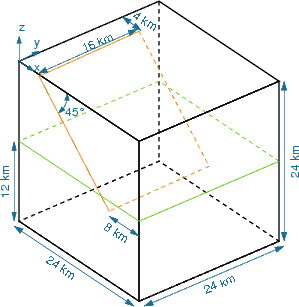
\includegraphics{figs/geometry}
    \caption{Geometry of model domain for simple model with
      strike-slip fault.}
  \end{center}
\end{figure}  

\subsubsection{Workflow}

The complete workflow used to create the input files for this tutorial
is shown in figure~\ref{fig:splitcube:workflow}. 

\begin{figure}[htbp]
  \begin{center}
    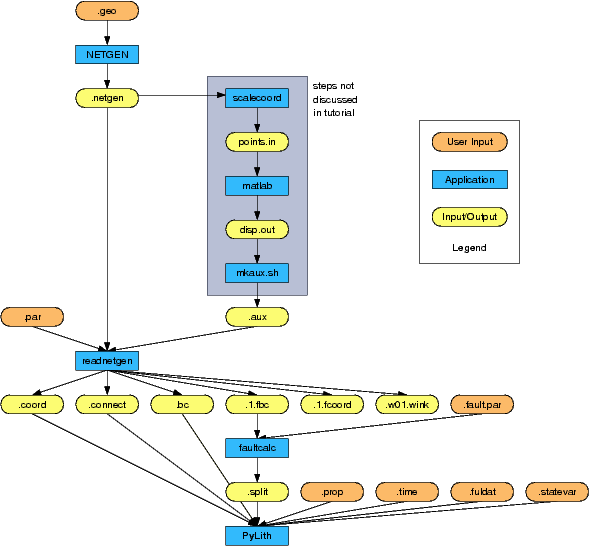
\includegraphics{figs/workflow}
    \caption{Workflow for setting up input files for example with
      simple strike-slip faylt.}
    \label{fig:splitcube:workflow}
  \end{center}
\end{figure}

\subsection{Download and unpack}

We will start by downloading the tutorial tarball and unpacking it.

\begin{enumerate}
\item Download the \href{http://www.geodynamics.org:8080/cig/Members/willic3/pylithusers/pylith0.8/pylith-0.8\_tutorials.tgz}{tutorial tarball}
  and unpack it in a location of your choosing.

  \begin{screen}
    \shellprompt\userinput{tar -zxvf pylith-0.8\_tutorials.tgz}
  \end{screen}
  
\item Go to the \directory{tutorials/splitcube} directory.
  The \directory{archive} directory contains all of the input and
  output files associated with this tutorial. We will copy input files
  from this directory into the \directory{workarea} directory. At each
  step, you can check to make sure your input and output agree with
  the files in the \directory{archive} directory. These files also
  allow you to start at an intermediate step as described in the next
  section.

  \begin{screen}
    \shellprompt\userinput{cd tutorials/splitcube}
  \end{screen}

\end{enumerate}

\subsection{Tutor}

Copy the \filename{tutor.py} script from the \directory{archive}
directory into the \directory{workarea} directory. 

\begin{tip}
  If you have run this tutorial previously, you may want to run
  \command{tutor.py} in mode "clean" with step "all" to clear out all
  old tutorial files.
\end{tip}

\begin{screen}
\shellprompt\userinput{cd workarea}
\shellprompt\userinput{cp ../archive/tutor.py .}
\shellprompt\userinput{./tutor.py -m clean -s all}
\end{screen}

\subsection{Generate the mesh}

In this step we will generate the finite-element mesh for the
benchmark problem using \application{NETGEN}.

\begin{enumerate}
\item In the \directory{splitcube/workarea} directory, run
  \command{tutor.py} for step "mesh" with mode "retrieve" to fetch the
  geometry file for \application{NETGEN}. You may also want to run
  \command{tutor.py} for this step with mode "clean" to clean out old
  files.

  \begin{screen}
    \shellprompt\userinput{./tutor.py -m retrieve -s mesh}
    \shellprompt\userinput{./tutor.py -m clean -s mesh}
  \end{screen}
  
\item Examine the \filename{splitcube.geo} file to see how the
  geometry for the problem is defined. Notice that the fault plane has
  been flagged with a boundary condition code. This will be used to
  associate boundary conditions with the fault surface and the
  associated nodes. We have not flagged the face on the plane x=0
  because we generate this boundary condition by hand. We also do not
  have to flag the other faces because they are traction-free, which
  is a natural boundary condition in the finite-element formulation.
\item Start up \application{NETGEN} by running \command{ng}.

  \begin{screen}
    \shellprompt\userinput{ng}
  \end{screen}
  
\item Select \guimenu{File}\guiselect\guimenuitem{Load Geometry}
  and select \filename{splitcube.geo}.
\item Click on \guibutton{Generate Mesh}.
\item Export the mesh to a file named \filename{splitcube.netgen},
  making sure the export filetype is "Neutral format".
\item You may now exit \application{NETGEN}.
\end{enumerate}

\subsection{Setup simulation input files}

In this step we will setup the PyLith input files for the mesh and
boundary conditions.

\begin{enumerate}
\item Run \command{tutor.py} for step "setup" with mode "retrieve" to
  fetch files from the archive.

  \begin{screen}
    \shellprompt\userinput{./tutor.py -m retrieve -s setup}
  \end{screen}
  
\item We will use a simple Fortran utility to generate PyLith
  input files from the \application{NETGEN} output.

  \begin{description}
  \item[\command{readnetgen}] A Fortran program to read
    \application{NETGEN} neutral format and create several of the
    input files needed by PyLith.
  \end{description}
  
\item Run the \command{readnetgen} utility program to process the
  \application{NETGEN} output file into PyLith compatible input files.
  It will ask for a root filename, enter \filename{splitcube}. This
  utility will generate the following files:
  \filename{splitcube.w01.wink}, \filename{splitcube.coord},
  \filename{splitcube.connect}, \filename{splitcube.bc},
  \filename{splitcube.1.fcoord}, \filename{splitcube.1.fbc}.

  \begin{screen}
    \shellprompt\userinput{../../utils/readnetgen}
    \prompt{\ Enter root name for all files.  Both input and}
    \prompt{\ output files will all have this prefix:}
    \userinput{splitcube}
  \end{screen}
  
\item The boundary conditions on the fault for this example are
  very simple. As a result, the \filename{splitcube.split} file was
  generated by hand. You should examine this file to see how a uniform
  left-lateral slip of 1.0 m is applied to the fault surface.

  \begin{warning}
    If you make any changes to \filename{splitcube.geo} or change the
    geometry within \application{NETGEN}, the split-node file
    \filename{splitcube.split} will no longer be correct and you will
    have to generate one yourself.  Note that it is also possible that
    a different version of \application{NETGEN} may provide a slightly
    different mesh, which would also be incompatible with the provided
    boundary conditions.
  \end{warning}
  
\item The external boundary conditions for this benchmark are simply
  pinned nodes on one face of the cube. Consequently, the boundary
  condition file was created by hand. You need to remove the one
  generated by the \command{readnetgen} utility which is empty and
  copy the hand-generated file from the archive directory.

  \begin{screen}
    \shellprompt\userinput{rm splitcube.bc}
    \shellprompt\userinput{cp ../archive/splitcube.bc .}
  \end{screen}
  
  \begin{warning}
    If you make any changes to \filename{splitcube.geo} or change the
    geometry within \application{NETGEN}, the boundary condition file
    \filename{splitcube.bc} will no longer be correct and you will
    have to generate one yourself.  Note that it is also possible that
    a different version of \application{NETGEN} may provide a slightly
    different mesh, which would also be incompatible with the provided
    boundary conditions.
  \end{warning}
\end{enumerate}

\subsection{Run the simulation on one processor}

In this step we will run the simulation on a single processor.

\begin{enumerate}
\item Run \command{tutor.py} for step "run1" with mode "retrieve" to
  fetch some parameter files from the archive.

  \begin{screen}
    \shellprompt\userinput{./tutor.py -m retrieve -s run1}
  \end{screen}
  
\item As defined in \filename{splitcube.time}, the simulation will
  only solve for the elastic solution. In \filename{splitcube.fuldat},
  we have not specified any time steps for output because in this
  problem we only compute the elastic solution, which is always
  included in the output. We define two materials with elastic
  behavior in \filename{splitcube.prop}. In
  \filename{splitcube.statevar} we choose to include total stress,
  total strain, incremental stress, and incremental strain in the
  output.
\item Run the simulation by executing \userinput{runbm.py -n 1}, where
  the 1 refers to the number of processors.

  \begin{tip}
    All of the input is echoed in the file \filename{splitcube.ascii}.
    You can check to make sure your input is digested correctly by
    examining this file. For large problems, this file can be quite
    large. You can suppress creation of this file using the command
    line argument \option{--scanner.asciiOutput=none} flag. On the
    other hand, for debugging purposes in small problems, you may wish
    to output everything, including the computed results, in this file
    using \option{--scanner.asciiOutput=full}.
  \end{tip}
  
  \begin{screen}
    \shellprompt\userinput{./runbm.py -n 1}
  \end{screen}
\end{enumerate}

\subsection{Visualize the single processor run}

Now it is time to visualize the results of the simulation. By default,
PyLith writes simulation output using
\href{http://help.avs.com/Express/doc/help/reference/dvmac/UCD\_Form.htm}{\application{AVS}
  UCD files}.  These can be read by several other visualization tools
besides \application{AVS}, e.g., \application{ParaView} and
\application{Iris Explorer}. We will use the open-source application
\application{ParaView} to visualize the results.
    
\begin{enumerate}
\item If necessary, run \command{tutor.py} for step "viz1" with mode
  "retrieve" to fetch the simulation output from the archive.

  \begin{screen}
    \shellprompt\userinput{./tutor.py -m retrieve -s viz1}
  \end{screen}
  
\item PyLith does not write complete UCD files. So the first step is
  to combine the mesh topology information with the output at a given
  time step into a complete UCD file. For example, use \command{cat}
  to merge the nodal coordinates file
  (\filename{splitcube\_1.0.mesh.inp}) and the nodal displacements at
  time step 10 file (\filename{splitcube\_1.0.mesh.time.00000.inp}) into
  \filename{splitcube\_1.0.mesh.t00000.inp}.

  \begin{screen}
    \shellprompt\userinput{cat splitcube\_1.0.mesh.inp splitcube\_1.0.mesh.time.00000.inp \(\backslash\)}
    \userinput{> splitcube\_1.0.mesh.t00000.inp}
\end{screen}

\item Start \application{ParaView} by executing \command{paraview}.

  \begin{screen}
    \shellprompt\userinput{paraview}
  \end{screen}
  
\item Load the UCD file that you just created by selecting
  \guimenu{File}\guiselect\guimenuitem{Open Data}. Select the file in
  the dialog box and the click the \guibutton{Open} button. Click the
  \guibutton{Accept} button. You should see a color rendering of the x
  displacements. You can use the mouse to rotate, translate, and zoom.
  Your image should look similar to the one in
  figure~\ref{fig::splitcube:xdisp:t0}.
        
  \begin{figure}[htbp]
    \begin{center}
      %\includegraphics{figs/xdisp_0}
      \caption{ParaView rendering of displacement in x-direction at
        time step 0 (elastic solution to the imposed dislocation) for
        the simple strike-slip example.}
      \label{fig:splitcube:xdisp:00}
    \end{center}
  \end{figure}
  
\item In the \guibutton{Display} tab, you can change several options,
  such as including a color bar, coloring a different component,
  interpolating colors, and changing the color map.
\item Let's show the displacements as vectors. Click on the calculator
  icon, and add the three displacement components together. Enter
  \begin{screen}
  XDispl*iHat + YDispl*jHat + ZDispl*kHat
  \end{screen}
  in the \guimenuitem{Calculator} box. Note the variable names are
  available by clicking on the \guibutton{scalars} button and the
  \guibutton{iHat}, \guibutton{jHat}, \guibutton{kHat} buttons are on
  the right side of the top row. Click on the \guibutton{Accept}
  button. To show the dataset as vectors, click on the
  \guibutton{glyph} button (looks like several dots) in the toolbar.
  After clicking the \guibutton{Accept} button, you should have a
  vector plot. You can turn on/off other datasets by clicking on the
  eye icon to the left of the dataset name. If you color the surfaces
  using the x-displacements field while also making the displacement
  vectors visible (colored using property), you should see an image
  similar to the one in figure~\ref{fig:splitcube:xdisp:vec:t0}.

  \begin{figure}[htbp]
    \begin{center}
      %\includegraphics{figs/splitcube_xdisp_vec_t0}
      \caption{ParaView rendering of displacement in x-direction and
        displacement vectors at time step 0 (elastic solution to the
        imposed dislocation) for the simple strike-slip example.}
      \label{fig:splitcube:xdisp:vec:t0}
    \end{center}
  \end{figure}      

\end{enumerate}

\subsection{Run the simulation on two processors}

In this step we will run the simulation on two processors. Even if
your machine only has one processor, a "multprocessor" job will run as
multiple processes on the single processor. In such cases, the job
will run slower than the single processor run, but the two processes
will behave independently as if they are on different processors.

\begin{enumerate}
\item Run \command{tutor.py} for step "run2" with mode "retrieve" to
  make sure all parameter files are available.

  \begin{screen}
    \shellprompt\userinput{./tutor.py -m retrieve -s run2}
  \end{screen}
  
\item The parameter files are the same as those in the single
  processor run. The \command{runbm.py} script will automatically take
  care of duplicating these files so that there is one for each
  processor.
\item Run the simulation by executing \command{runbm.py -n 2}, where
  the 2 refers to the number of processors.

  \begin{screen}
    \shellprompt\userinput{./runbm.py -n 2}
  \end{screen}
\end{enumerate}

\subsection{Visualize the two processor run}

PyLith does not currently support parallel output, so each processor
writes its UCD output to a different file. This means that you need to
form complete UCD files for each processor and then load each one into
\application{ParaView}.

\begin{enumerate}
\item If necessary, run \command{tutor.py} for step "viz2" with mode
  "retrieve" to fetch the simulation output from the archive.

  \begin{screen}
    \shellprompt\userinput{./tutor.py -m retrieve -s viz2}
  \end{screen}
  
\item As in the case of the single processor run, the first step is to
  combine the mesh topology information with the output at a given
  time step into a complete UCD file. Because PyLith writes the output
  from each processor into a different file, we must run \command{cat}
  twice to create UCD files for each processor.

  \begin{screen}
    \shellprompt\userinput{cat splitcube\_2.0.mesh.inp splitcube\_2.0.mesh.time.00000.inp \(\backslash\)}
      \userinput{> splitcube\_2.0.mesh.t00000.inp}
    \shellprompt\userinput{cat splitcube\_2.1.mesh.inp splitcube\_2.1.mesh.time.00000.inp \(\backslash\)}
      \userinput{> splitcube\_2.1.mesh.t00000.inp}
  \end{screen}

\item Start \application{ParaView} by executing \command{paraview}.

  \begin{screen}
    \shellprompt\userinput{paraview}
  \end{screen}
  
\item Load the UCD files that you just created by selecting
  \guimenu{File}\guiselect\guimenuitem{Open Data}. Select the file in
  the dialog box and the click the \guibutton{Open} button. Click the
  \guibutton{Accept} button. You can now visualize the datasets just
  like you did for the single processor case.
\item You can merge the datasets from the different processors by
  selecting \guimenu{Filter}\guiselect\guimenuitem{Append}. Doing so
  will allow you to operate on the data from all of the processors
  simultaneously instead of having to repeat any processing for every
  processor.
\end{enumerate}

\section{Tutorial Using Reverse-Slip Without Gravity Benchmark}

\subsection{Overview}

In this tutorial, we will walk through the steps necessary to
construct, run, and view the results of a benchmark problem involving
reverse slip on a dipping fault. This problem examines the
viscoelastic (Maxwell) relaxation of stress from a single, finite,
reverse-slip earthquake in 3-D without body forces.


\subsection{Problem Description}

The model domain is a cube with edges 24 km long (0 km $\leq$ x $\leq$
24 km; 0 km $\leq$ y $\leq$ 24 km; -24 km $\leq$ z $\leq$ 0) and
is composed of two materials. One material occupies the top-half of
the domain, -12 km $\leq$ z $\leq$ 0 km, while the other occupies
the lower half, -24 km $\leq$ z $<$ 12 km. Both materials are Poisson
solids with Lame's constants ($\mu$ and $\lambda$) equal to 30 GPa and
Maxwell viscoelastic properties. The top layer has a viscosity of
$10^25$ Pa-s (and is essentially elastic) while the bottom layer has a
viscosity of $10^18$ Pa-s.

The reverse fault dips at an angle of 45 degrees. The top of the fault
sits at x = 4 km with the bottom of the fault at x = 20 km. The fault
surface is confined to the region 0 km $\leq$ y $\leq$ 16 km and -16
km $\leq$ z $\leq$ 0 km. The slip distribution is 1.0 m of uniform
thrust motion for -12 km $\leq$ z with a linear taper to 0 at z = -16
km.

The plane y=0 is a plane of symmetry, so the y-DOF displacements on
this face are zero. The boundary conditions on the other lateral faces
and bottom of the mesh are the displacements from the analytical
elastic solution. These displacements are held fixed through time.

\begin{figure}
  \begin{center}
    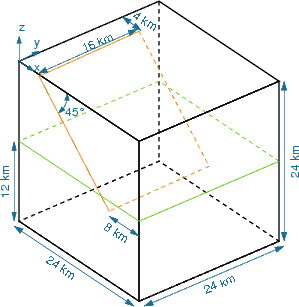
\includegraphics{figs/geometry}
    \caption{Geometry of model domain for reverse-slip benchmark.}
  \end{center}
\end{figure}  

\subsubsection{Workflow}

The complete workflow used to create the input files for this tutorial
is shown in figure~\ref{fig:bmrsnog:workflow}. Because some of the
steps involve commercial software (e.g., Matlab), we will skip those
steps in this tutorial.

\begin{figure}[htbp]
  \begin{center}
    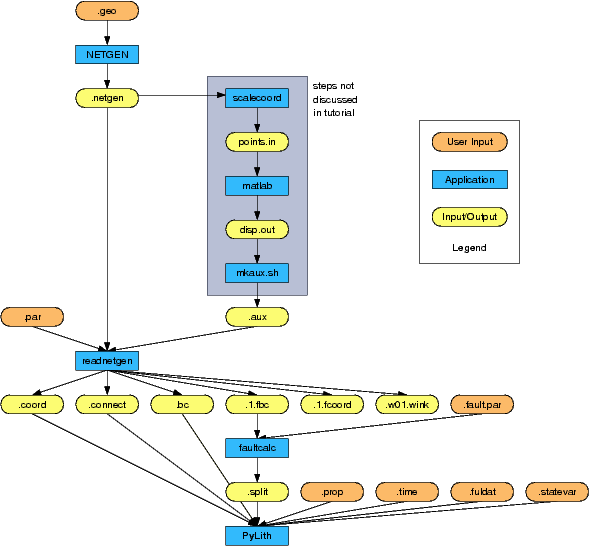
\includegraphics{figs/workflow}
    \caption{Workflow for setting up input files for benchmark with reverse
      slip and no gravity.}
    \label{fig:bmrsnog:workflow}
  \end{center}
\end{figure}

\subsection{Download and unpack}

We will start by downloading the tutorial tarball and unpacking it.

\begin{enumerate}
\item Download the \href{http://www.geodynamics.org:8080/cig/Members/willic3/pylithusers/pylith0.8/pylith-0.8\_tutorials.tgz}{tutorial
    tarball}
  and unpack it in a location of your choosing.

  \begin{screen}
    \shellprompt\userinput{tar -zxvf pylith-0.8\_tutorials.tgz}
  \end{screen}
  
\item Go to the \directory{tutorials/reversenog} directory.
  The \directory{archive} directory contains all of the input and
  output files associated with this tutorial. We will copy input files
  from this directory into the \directory{workarea} directory. At each
  step, you can check to make sure your input and output agree with
  the files in the \directory{archive} directory. These files also
  allow you to start at an intermediate step as described in the next
  section.

  \begin{screen}
    \shellprompt\userinput{cd tutorials/reversenog}
  \end{screen}

\end{enumerate}

\subsection{Tutor}

Copy the \filename{tutor.py} script from the \directory{archive}
directory into the \directory{workarea} directory. 

\begin{tip}
  If you have run this tutorial previously, you may want to run
  \command{tutor.py} in mode "clean" with step "all" to clear out all
  old tutorial files.
\end{tip}

\begin{screen}
\shellprompt\userinput{cd workarea}
\shellprompt\userinput{cp ../archive/tutor.py .}
\shellprompt\userinput{./tutor.py -m clean -s all}
\end{screen}

\subsection{Generate the mesh}

In this step we will generate the finite-element mesh for the
benchmark problem using \application{NETGEN}.

\begin{enumerate}
\item In the \directory{reversenog/workarea} directory, run
  \command{tutor.py} for step "mesh" with mode "retrieve" to fetch the
  geometry file for \application{NETGEN}. You may also want to run
  \command{tutor.py} for this step with mode "clean" to clean out old
  files.

  \begin{screen}
    \shellprompt\userinput{./tutor.py -m retrieve -s mesh}
    \shellprompt\userinput{./tutor.py -m clean -s mesh}
  \end{screen}
  
\item Examine the \filename{bmrsnog.geo} file to see how the geometry
  for the problem is defined. Notice that the different planes have
  been flagged with different boundary condition codes. These will be
  used to associate boundary conditions with surfaces and element
  nodes.
\item Start up \application{NETGEN} by running \command{ng}.

  \begin{screen}
    \shellprompt\userinput{ng}
  \end{screen}
  
\item Select \guimenu{File}\guiselect\guimenuitem{Load Geometry}
  and select \filename{bmrsnog.geo}.
\item Click on \guibutton{Generate Mesh}.
\item Export the mesh to a file named \filename{bmrsnog.netgen},
  making sure the export filetype is "Neutral format".
\item You can now exit \application{NETGEN}.
\end{enumerate}

\subsection{Setup simulation input files}

In this step we will setup the PyLith input files for the mesh and
boundary conditions.

\begin{enumerate}
\item Run \command{tutor.py} for step "setup" with mode "retrieve" to
  fetch files from the archive.

  \begin{screen}
    \shellprompt\userinput{./tutor.py -m retrieve -s setup}
  \end{screen}
  
\item We will use two simple Fortran utilities to generate PyLith
  input files from the \application{NETGEN} output.

  \begin{description}
  \item[\command{readnetgen}] A Fortran program to read
    \application{NETGEN} neutral format and create several of the
    input files needed by PyLith.
  \item[\command{faultcalc}] A Fortran program to compute split node
    displacements using second order polynomials over specified
    regions.
  \end{description}
  
\item Run the \command{readnetgen} utility program to process the
  \application{NETGEN} output file into PyLith compatible input files.
  It will ask for a root filename, enter \filename{bmrsnog}. This
  utilitiy will generate the following files:
  \filename{bmrsnog.w01.wink}, \filename{bmrsnog.coord},
  \filename{bmrsnog.connect}, \filename{bmrsnog.bc},
  \filename{bmrsnog.1.fcoord}, \filename{bmrsnog.1.fbc}.

  \begin{screen}
    \shellprompt\userinput{../../utils/readnetgen}
    \prompt{\ Enter root name for all files.  Both input and}
    \prompt{\ output files will all have this prefix:}
    \userinput{bmrsnog}
  \end{screen}
  
\item The boundary conditions on the fault for this benchmark are
  somewhat complex. The utility program \command{faultcalc} creates
  split node boundary conditions over specified regions, using
  functions based on second degree polynomials. The
  \command{readnetgen} program has already produced the main input for
  \command{faultcalc} -- split node definitions in
  \filename{bmrsnog.1.fbc} and nodal coordinates in
  \filename{bmrsnog.coord}. The file \filename{bmrsnog.fault.par}
  contains the polynomial coefficients for this benchmark problem. Run
  \command{faultcalc} to get the \filename{bmrsnog.split} file that
  PyLith needs as input.

  \begin{screen}
    \shellprompt\userinput{../../utils/faultcalc p=bmrsnog.fault.par n=bmrsnog.coord \(\backslash\)}
      \userinput{i=bmrsnog.1.fbc o=bmrsnog.split}
  \end{screen}
  
\item The external boundary conditions for this benchmark are also
  complicated and require computing the displacements for the
  analytical elastic solution at each finite element node on the
  external boundaries. The file specifying these boundary conditions,
  \filename{bmrsnog.bc}, was produced with \command{readnetgen} using
  the \filename{bmrsnog.aux} file (which contains precomputed
  displacements for the external boundaries for the mesh produced from
  the \filename{bmrsnog.geo} geometry).

  \begin{warning}
    If you make any changes to \filename{bmrsnog.geo} or change the
    geometry within \application{NETGEN}, the boundary condition file
    \filename{bmrsnog.bc} will no longer be correct and you will have
    to generate one yourself.  Note that it is also possible that a
    different version of \application{NETGEN} may provide a slightly
    different mesh, which would also be incompatible with the provided
    boundary conditions.
  \end{warning}
\end{enumerate}

\subsection{Run the simulation on one processor}

In this step we will run the simulation on a single processor.

\begin{enumerate}
\item Run \command{tutor.py} for step "run1" with mode "retrieve" to
  fetch some parameter files from the archive.

  \begin{screen}
    \shellprompt\userinput{./tutor.py -m retrieve -s run1}
  \end{screen}
  
\item In \filename{bmrsnog.fuldat}, we have specified that we want
  full output at time steps 10, 50, and 100. We define six materials
  with both elastic and viscoelastic behavior in
  \filename{bmrsnog.prop}. In \filename{bmrsnog.statevar} we choose to
  include total stress, total strain, incremental stress, and
  incremental strain in the output. As defined in
  \filename{bmrsnog.time}, the simulation will have 100 time steps of
  0.1 year each.
\item Run the simulation by executing \userinput{runbm.py -n 1}, where
  the 1 refers to the number of processors.

  \begin{tip}
    All of the input is echoed in the file \filename{bmrsnog.ascii}.
    You can check to make sure your input is digested correctly by
    examining this file. For large problems, this file can be quite
    large. You can suppress creation of this file using the command
    line argument \option{--scanner.asciiOutput=none} flag. On the
    other hand, for debugging purposes in small problems, you may wish
    to output everything, including the computed results, in this file
    using \option{--scanner.asciiOutput=full}.
  \end{tip}
  
  \begin{screen}
    \shellprompt\userinput{./runbm.py -n 1}
  \end{screen}
\end{enumerate}

\subsection{Visualize the single processor run}

Now it is time to visualize the results of the simulation. By default,
PyLith writes simulation output using
\href{http://help.avs.com/Express/doc/help/reference/dvmac/UCD\_Form.htm}{\application{AVS}
  UCD files}.  These can be read by several other visualization tools
besides \application{AVS}, e.g., \application{ParaView} and
\application{Iris Explorer}. We will use the open-source application
\application{ParaView} to visualize the results.
    
\begin{enumerate}
\item If necessary, run \command{tutor.py} for step "viz1" with mode
  "retrieve" to fetch the simulation output from the archive.

  \begin{screen}
    \shellprompt\userinput{./tutor.py -m retrieve -s viz1}
  \end{screen}
  
\item PyLith does not write complete UCD files. So the first step is
  to combine the mesh topology information with the output at a given
  time step into a complete UCD file. For example, use \command{cat}
  to merge the nodal coordinates file
  (\filename{bmrsnog\_1.0.mesh.inp}) and the nodal displacements at
  time step 10 file (\filename{bmrsnog\_1.0.mesh.time.00010.inp}) into
  \filename{bmrsnog\_1.0.mesh.t00010.inp}.

  \begin{screen}
    \shellprompt\userinput{cat bmrsnog\_1.0.mesh.inp bmrsnog\_1.0.mesh.time.00010.inp \(\backslash\)}
    \userinput{> bmrsnog\_1.0.mesh.t00010.inp}
\end{screen}

\item Start \application{ParaView} by executing \command{paraview}.

  \begin{screen}
    \shellprompt\userinput{paraview}
  \end{screen}
  
\item Load the UCD file that you just created by selecting
  \guimenu{File}\guiselect\guimenuitem{Open Data}. Select the file in
  the dialog box and the click the \guibutton{Open} button. Click the
  \guibutton{Accept} button. You should see a color rendering of the x
  displacements. You can use the mouse to rotate, translate, and zoom.
  Your image should look similar to the one in
  figure~\ref{fig::bmrsnog:xdisp:t10}.
        
  \begin{figure}[htbp]
    \begin{center}
      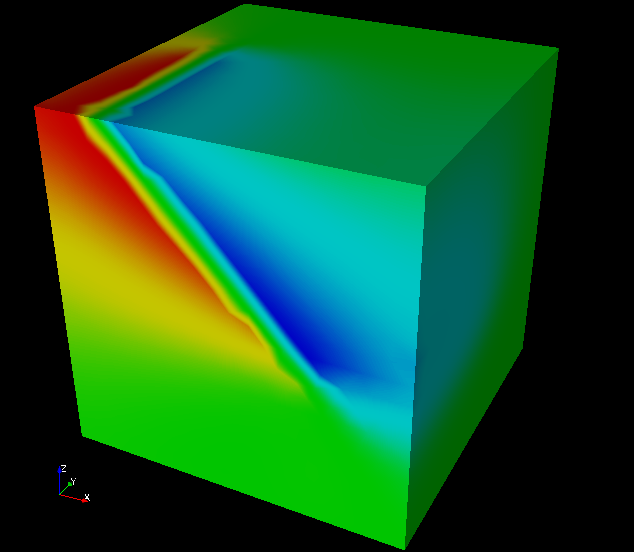
\includegraphics{figs/xdisp_t10}
      \caption{ParaView rendering of displacement in x-direction at
          time step 10 (10 yrs after imposed dislocation) for the
          reverse slip without gravity benchmark.}
      \label{fig:bmrsnog:xdisp:t10}
    \end{center}
  \end{figure}
  
\item In the \guibutton{Display} tab, you can change several options,
  such as including a color bar, coloring a different component,
  interpolating colors, and changing the color map.
\item Let's show the displacements as vectors. Click on the calculator
  icon, and add the three displacement components together. Enter
  \begin{screen}
  XDispl*iHat+YDispl*jHat+ZDispl*kHat
  \end{screen}
  in the \guimenuitem{Calculator} box. Note the variable names are
  available by clicking on the \guibutton{scalars} button and the
  \guibutton{iHat}, \guibutton{jHat}, \guibutton{kHat} buttons are on
  the right side of the top row. Click on the \guibutton{Accept}
  button. To show the dataset as vectors, click on the
  \guibutton{glyph} button (looks like several dots) in the toolbar.
  After clicking the \guibutton{Accept} button, you should have a
  vector plot. You can turn on/off other datasets by clicking on the
  eye icon to the left of the dataset name. If you color the surfaces
  using the x-displacements field while also making the displacement
  vectors visible (colored using property), you should see an image
  similar to the one in figure~\ref{fig:bmrsnog:xdisp:vec:t10}.

  \begin{figure}[htbp]
    \begin{center}
      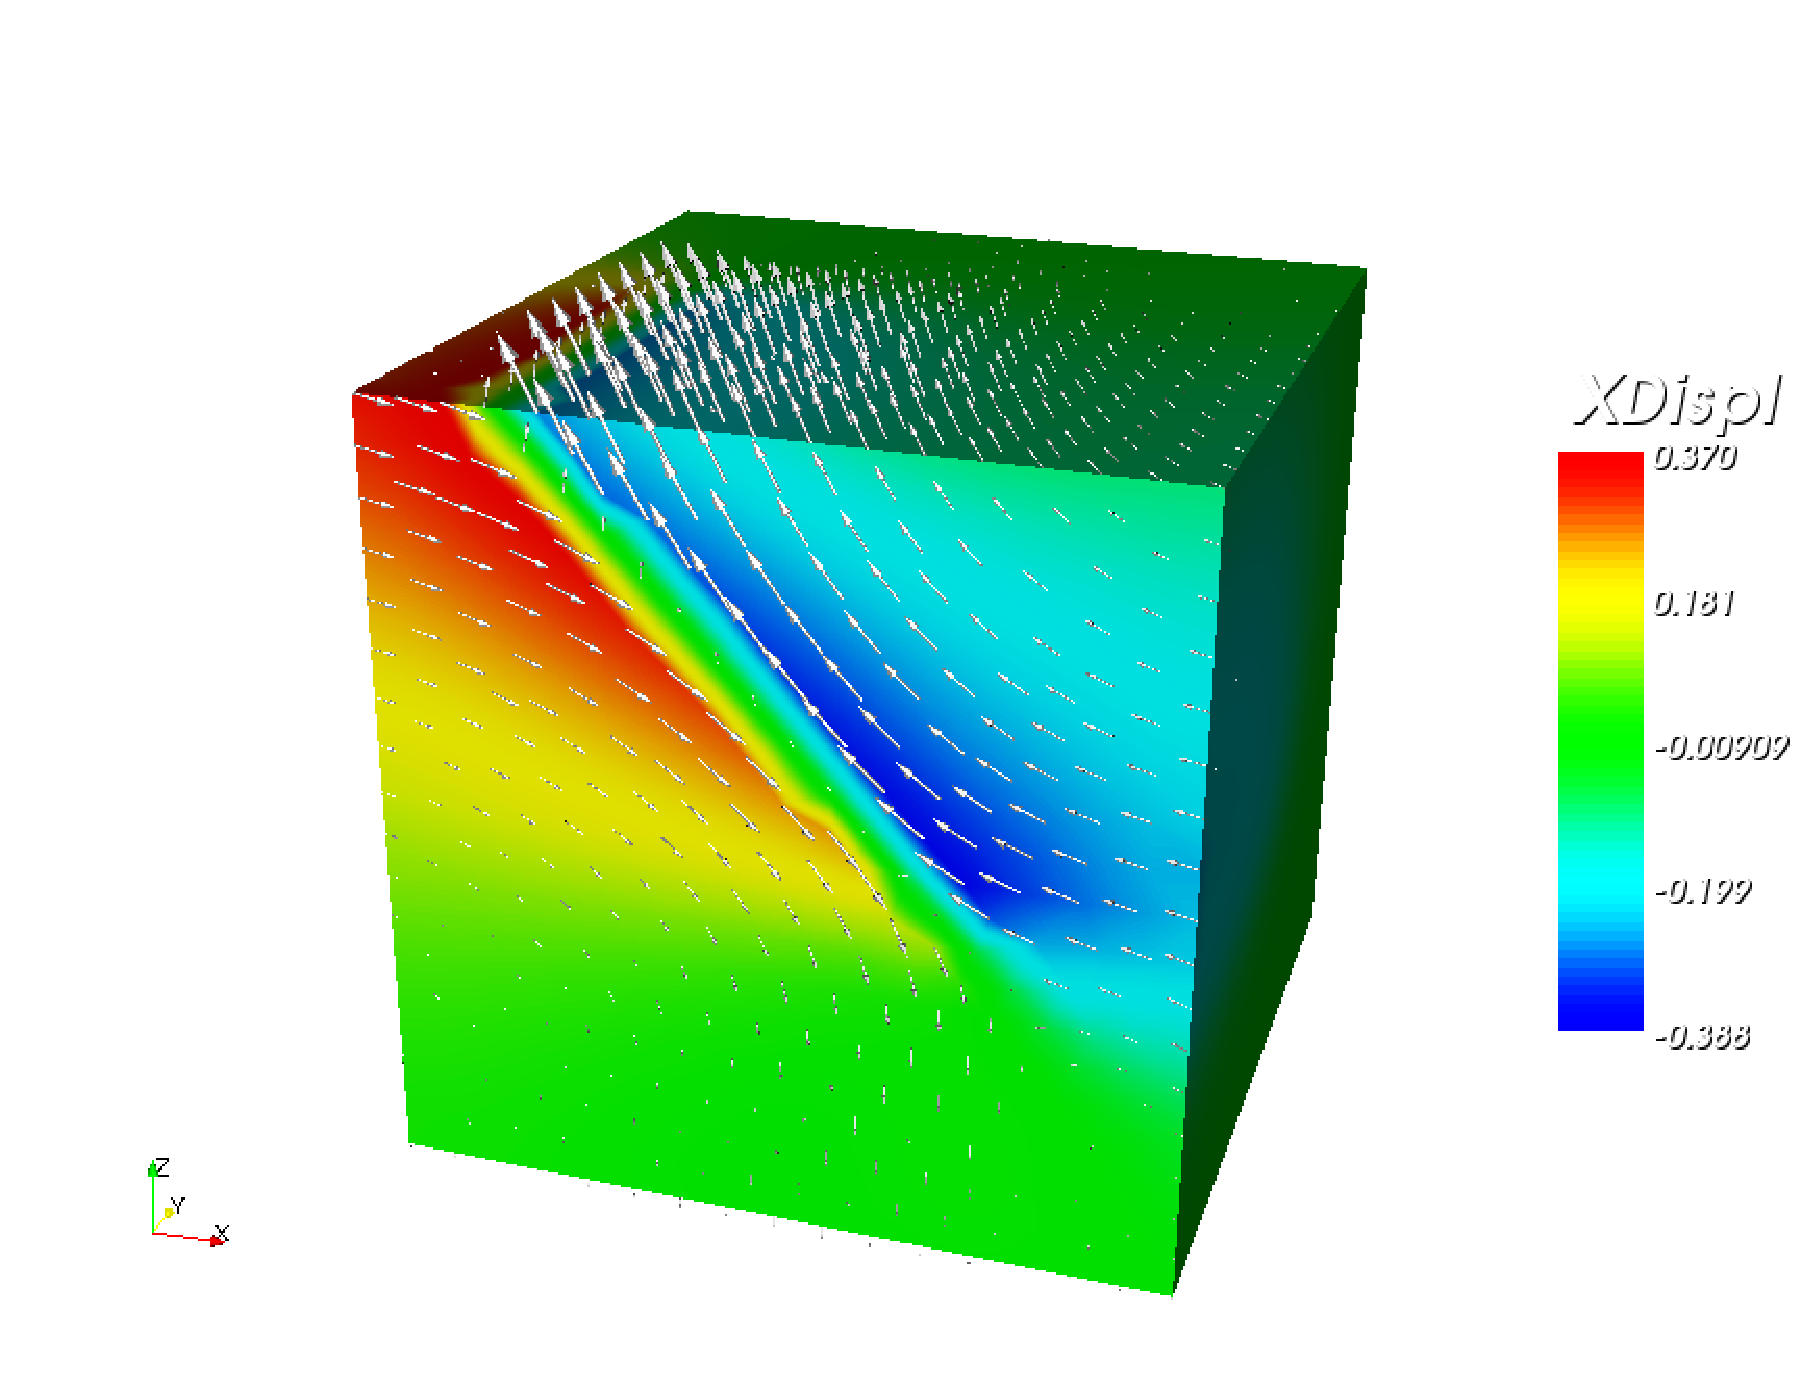
\includegraphics{figs/xdisp_vec_t10}
      \caption{ParaView rendering of displacement in x-direction and
        displacement vectors at time step 10 (10 yrs after imposed
        dislocation) for the reverse slip without gravity
        benchmark.}
      \label{fig:bmrsnog:xdisp:vec:t10}
    \end{center}
  \end{figure}      

\end{enumerate}

\subsection{Run the simulation on two processors}

In this step we will run the simulation on two processors. Even if
your machine only has one processor, a "multprocessor" job will run as
multiple processes on the single processor. In such cases, the job
will run slightly slower than the single processor run, but the two
processes will behave independently as if they are on different
processors.

\begin{enumerate}
\item Run \command{tutor.py} for step "run2" with mode "retrieve" to
  make sure all parameter files are available.

  \begin{screen}
    \shellprompt\userinput{./tutor.py -m retrieve -s run2}
  \end{screen}
  
\item The parameter files are the same as those in the single
  processor run. The \command{runbm} script will automatically take
  care of duplicating these files so that there is one for each
  processor.
\item Run the simulation by executing \command{runbm.py -n 2}, where
  the 2 refers to the number of processors.

  \begin{screen}
    \shellprompt\userinput{./runbm.py -n 2}
  \end{screen}
\end{enumerate}

\subsection{Visualize the two processor run}

PyLith does not currently support parallel output, so each processor
writes its UCD output to a different file. This means that you need to
form complete UCD files for each processor and then load each one into
\application{ParaView}.

\begin{enumerate}
\item If necessary, run \command{tutor.py} for step "viz2" with mode
  "retrieve" to fetch the simulation output from the archive.

  \begin{screen}
    \shellprompt\userinput{./tutor.py -m retrieve -s viz2}
  \end{screen}
  
\item As in the case of the single processor run, the first step is to
  combine the mesh topology information with the output at a given
  time step into a complete UCD file. Because PyLith writes the output
  from each processor into a different file, we must run \command{cat}
  twice to create UCD files for each processor.

  \begin{screen}
    \shellprompt\userinput{cat bmrsnog\_2.0.mesh.inp bmrsnog\_2.0.mesh.time.00010.inp \(\backslash\)}
      \userinput{> bmrsnog\_2.0.mesh.t00010.inp}
    \shellprompt\userinput{cat bmrsnog\_2.1.mesh.inp bmrsnog\_2.1.mesh.time.00010.inp \(\backslash\)}
      \userinput{> bmrsnog\_2.1.mesh.t00010.inp}
  \end{screen}

\item Start \application{ParaView} by executing \command{paraview}.

  \begin{screen}
    \shellprompt\userinput{paraview}
  \end{screen}
  
\item Load the UCD files that you just created by selecting
  \guimenu{File}\guiselect\guimenuitem{Open Data}. Select the file in
  the dialog box and the click the \guibutton{Open} button. Click the
  \guibutton{Accept} button. You can now visualize the datasets just
  like you did for the single processor case.
\item You can merge the datasets from the different processors by
  selecting \guimenu{Filter}\guiselect\guimenuitem{Append}. Doing so
  will allow you to operate on the data from all of the processors
  simultaneously instead of having to repeat any processing for every
  processor.
\end{enumerate}



\chapter{\label{cha:Benchmarks}Benchmarks}


\section{Overview}

The Crustal Deformation Modeling and Earthquake Source Physics Focus
Groups within the Southern California Earthquake Center and the Short-Term
Tectonics Working Group within CIG have developed a suite of benchmarks
to test the accuracy and performance of 3D numerical codes for quasi-static
crustal deformation and earthquake rupture dynamics. The benchmark
definitions for the quasi-static crustal deformation benchmarks are
posted on the CIG website at Short-Term Tectonics Benchmarks \url{geodynamics.org/cig/workinggroups/short/workarea/benchmarks/}
and the definitions for the earthquake rupture benchmarks are posted
on the SCEC website \url{scecdata.usc.edu/cvws/cgi-bin/cvws.cgi}.
This suite of benchmarks permits evaluating the relative performance
of different types of basis functions, quadrature schemes, and discretizations
for geophysical applications. The files needed to run the 3D benchmarks
are in the CIG GitHub Repository \url{https://github.com/geodynamics/pylith_benchmarks}.
In addition to evaluating the efficiency and accuracy of numerical
codes, the benchmarks also make good test problems, where users can
perform simulations based on actual geophysical problems. The benchmarks
are performed at various resolutions and using different element types.
By comparing the runtime and accuracy for different resolutions and
element types, users can evaluate which combination will be best for
their problems of interest.


\section{\label{sec:benchmarks:strikeslip}Strike-Slip Benchmark}

This benchmark problem computes the viscoelastic (Maxwell) relaxation
of stresses from a single, finite, strike-slip earthquake in 3D without
gravity.  Dirichlet boundary conditions equal to the analytical elastic
solution are imposed on the sides of a cube with sides of length 24
km. Anti-plane strain boundary conditions are imposed at y = 0, so
the solution is equivalent to that for a domain with a 48 km length
in the y direction. We can use the analytical solution of \cite{Okada:1992}
both to apply the boundary conditions and to compare against the numerically-computed
elastic solution.




\subsection{Problem Description}

Figure \ref{fig:benchmark:strikeslip:geometry} shows the geometry
of the strike-slip fault (red surface) embedded in the cube consisting
of an elastic material (yellow block) over a Maxwell viscoelastic
material (blue block). 
\begin{description}
\item [{Domain}] The domain spans the region
\begin{gather*}
0\leq x\leq24\ km,\\
0\leq y\leq24\ km,\\
-24\ km\leq z\leq0.
\end{gather*}
The top (elastic) layer occupies the region $-12\ km\ \leq z\leq0$
and the bottom (viscoelastic) layer occupies the region $-24\ km\ \leq z\leq-12\ km$.
\item [{Material~properties}] The material is a Poisson solid with a shear
modulus of 30 GPa. The domain is modeled using an elastic isotropic
material for the top layer and a Maxwell viscoelastic material for
the bottom layer. The bottom layer has a viscosity of 1.0e+18 Pa-s.
\item [{Fault}] The fault is a vertical, right-lateral strike-slip fault.
The strike is parallel to the y-direction at the center of the model:
\begin{gather*}
x=12\ km,\\
0\leq y\leq16\ km,\\
-16\ km\leq z\leq0.
\end{gather*}
Uniform slip of 1 m is applied over the region $0\leq y\leq12\ km$
and $-12\ km\leq z\leq0$ with a linear taper to 0 at y = 16 km and
z = -16 km. The tapered region is the light red portion of the fault
surface in Figure \ref{fig:benchmark:strikeslip:geometry}. In the
region where the two tapers overlap, each slip value is the minimum
of the two tapers (so that the taper remains linear).
\item [{Boundary~conditions}] Bottom and side displacements are set to
the elastic analytical solution, and the top of the model is a free
surface. There are two exceptions to these applied boundary conditions.
The first is on the y=0 plane, where y-displacements are left free
to preserve symmetry, and the x- and z-displacements are set to zero.
The second is along the line segment between (12, 0, -24) and (12,
24, -24), where the analytical solution blows up in some cases. Along
this line segment, all three displacement components are left free.
\item [{Discretization}] The model is discretized with nominal spatial
resolutions of 1000 m, 500 m, and 250 m.
\item [{Basis~functions}] We use trilinear hexahedral cells and linear
tetrahedral cells.
\item [{Solution}] We compute the error in the elastic solution and compare
the solution over the domain after 0, 1, 5, and 10 years.
\end{description}
\noindent \begin{center}
\begin{figure}[H]
\begin{centering}
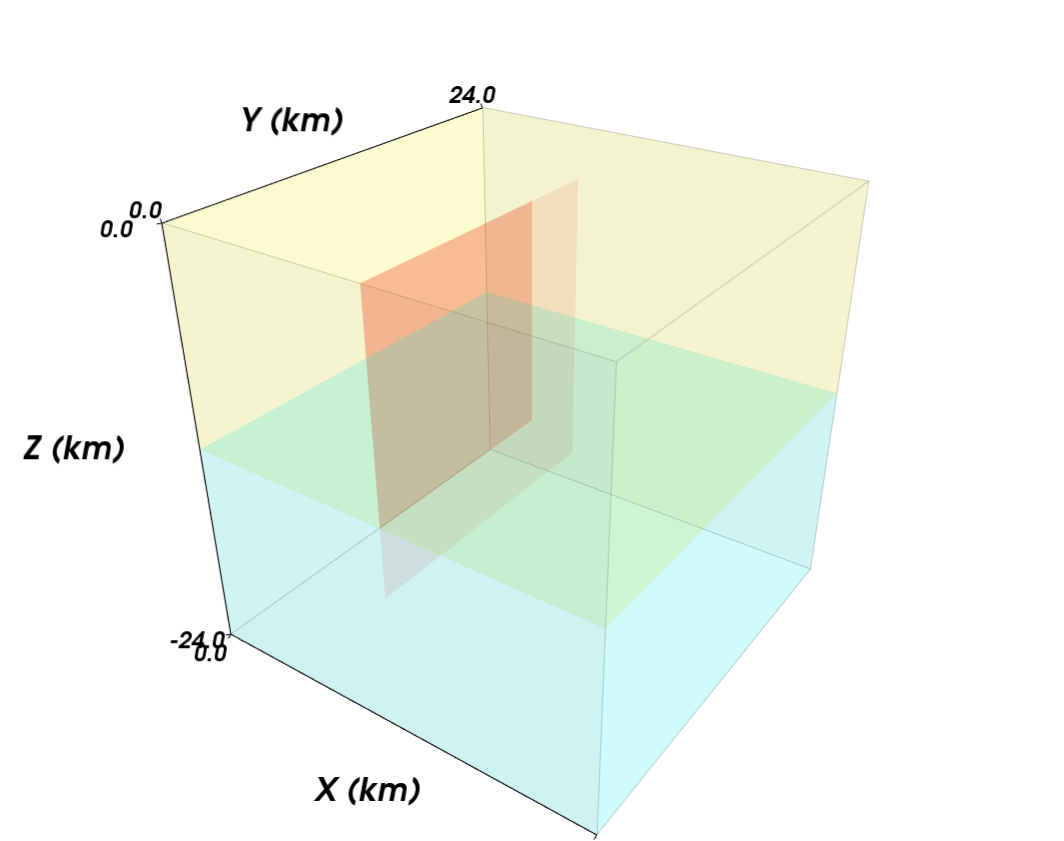
\includegraphics[scale=0.33]{benchmarks/strikeslip/figs/geometry}
\par\end{centering}

\caption{Geometry of strike-slip benchmark problem.\label{fig:benchmark:strikeslip:geometry}}
\end{figure}

\par\end{center}


\subsection{Running the Benchmark}

After checking out the benchmark files from the CIG SVN repository,
change to the \texttt{quasistatic/strikeslip} directory. Decompress
the gzipped files in the meshes and parameters directories,
\begin{lyxcode}
gunzip~meshes/{*}.gz~parameters/{*}.gz
\end{lyxcode}
Change to the parameters directory. Each benchmark uses three \texttt{.cfg}
files: \texttt{pylithapp.cfg}, a mesher related file (\texttt{strikeslip\_cubit.cfg}
or \texttt{strikeslip\_lagrit.cfg}), and a resolution and cell related
file (e.g., \texttt{strikeslip\_hex8\_1000m.cfg}). A few examples
of running the benchmarks (elastic solution only) are
\begin{lyxcode}
pylith~strikeslip\_cubit.cfg~strikeslip\_hex8\_1000m.cfg

pylith~strikeslip\_cubit.cfg~strikeslip\_hex8\_0500m.cfg

pylith~strikeslip\_lagrit.cfg~strikeslip\_tet4\_1000m.cfg
\end{lyxcode}
To run the time-dependent (viscoelastic) problem, it is necessary
to append \texttt{timedep.cfg} to the above commands, for example
\begin{lyxcode}
pylith~strikeslip\_cubit.cfg~strikeslip\_hex8\_1000m.cfg~timedep.cfg
\end{lyxcode}
This will run the problem for 10 years, using a time-step size of
0.1 years, and results will be output for each year. The benchmarks
at resolutions of 1000 m, 500 m, and 250 m require  approximately
150 MB, 960 MB, and 8 GB, respectively.


\subsection{Benchmark Results}

Figure \ref{fig:benchmark:strikeslip:solution} shows the displacement
field from the simulation with hexahedral cells using trilinear basis
functions at a resolution of 1000 m. For each resolution and set of
basis functions, we measure the accuracy by comparing the numerical
solution against the semi-analytical Okada solution \cite{Okada:1992}.
We also compare the accuracy and runtime across resolutions and different
cell types. This provides practical information about what cell types
and resolutions are required to achieve a given level of accuracy
with the shortest runtime.

\begin{figure}
\begin{centering}
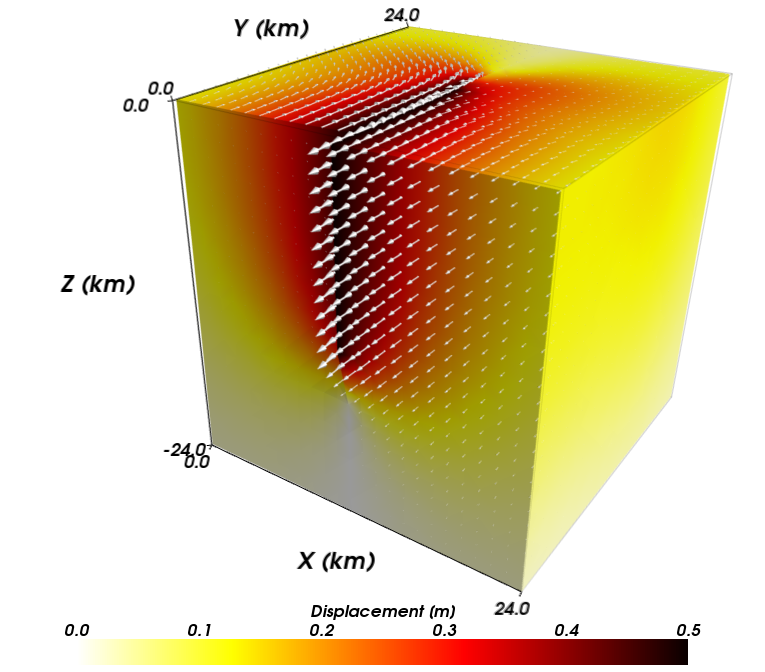
\includegraphics[scale=0.33]{benchmarks/strikeslip/figs/soln}
\par\end{centering}

\caption{Displacement field for strike-slip benchmark problem.\label{fig:benchmark:strikeslip:solution}}
\end{figure}



\subsubsection{Solution Accuracy}

We quantify the error in the finite-element solution by integrating
the L2 norm of the difference between the finite-element solution
 and the semi-analytical solution evaluated at the quadrature points.
We define the local error (error for each finite-element cell) to
be
\begin{equation}
\epsilon_{local}=\frac{1}{V_{cell}}\sqrt{\intop_{cell}\left(u_{i}^{t}-u_{i}^{fem}\right)^{2}\: dV},
\end{equation}
where $u_{i}^{t}$ is the ith component of the displacement field
for the semi-analytical  solution, and $u_{i}^{fem}$ is the ith component
of the displacement field for the finite-element  solution.  Taking
the square root of the L2 norm and normalizing by  the volume of the
cell results in an error metric with dimensions of length.  This roughly
corresponds to the error in the magnitude of the displacement field
in the finite element solution. We define the global error in a similar
fashion,
\begin{equation}
\epsilon_{global}=\frac{1}{V_{domain}}\sqrt{\intop_{domain}\left(u_{i}^{t}-u_{i}^{fem}\right)^{2}\: dV},
\end{equation}
 where we sum the L2 norm computed for the local error over all of
the  cells before taking the square root and dividing by the volume
of the domain. CIG has developed a package called Cigma \url{geodynamics.org/cig/software/packages/cs/cigma}
that computes these local and global error metrics.

Figures \ref{fig:benchmark:strikeslip:tet4:1000m} through \ref{fig:benchmark:strikeslip:hex8:250m}
show the local error for each of the three resolutions and two cell
types. The error decreases with decreasing cell size as expected for
a converging solution. The largest errors, which approach 1 mm for
1 m of slip for a discretization size of 250 m, occur where the gradient
in slip is discontinuous at the boundary between the region of uniform
slip and linear taper in slip. The linear basis functions cannot match
this higher order variation. The trilinear basis functions in the
hexahedral element provide more terms in the polynomial defining the
variation in the displacement field within each cell compared to the
linear basis functions for the tetrahedral cell. Consequently, for
this problem the error for the hexahedral cells at a given resolution
is smaller than that for the tetrahedral cells. Both sets of cell
types and basis functions provide the same rate of convergence as
shown in Figure \vref{fig:benchmark:strikeslip:convergence}.

\noindent \begin{center}
\begin{figure}[H]
\begin{centering}
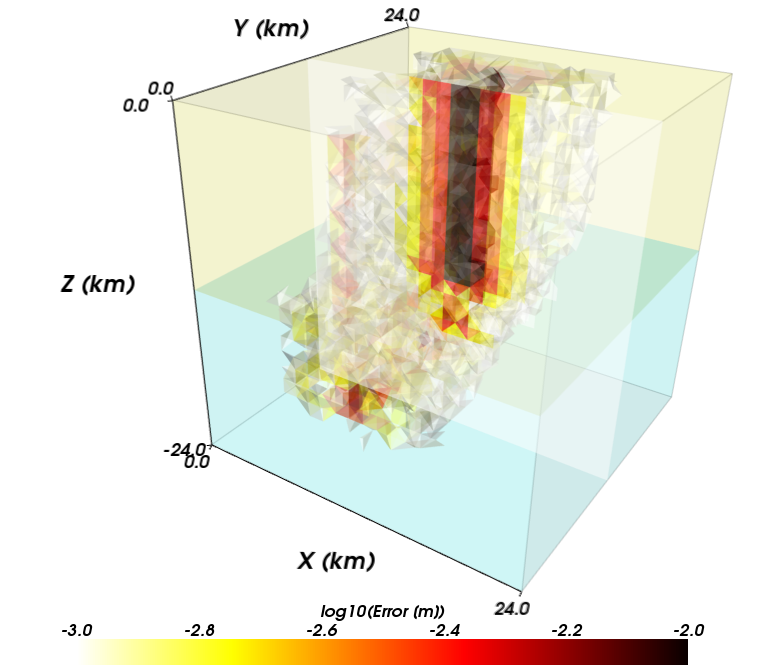
\includegraphics[scale=0.33]{benchmarks/strikeslip/figs/error_tet4_1000m}
\par\end{centering}

\caption{Local error for strike-slip benchmark problem with tetrahedral cells
and linear basis functions with a uniform discretization size of 1000
m.\label{fig:benchmark:strikeslip:tet4:1000m}}
\end{figure}

\par\end{center}

\noindent \begin{center}
\begin{figure}[H]
\begin{centering}
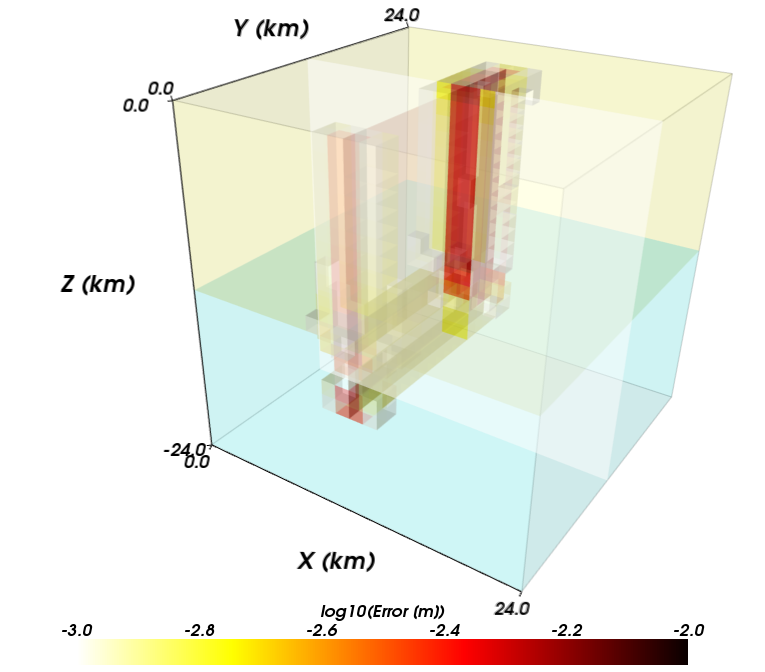
\includegraphics[scale=0.33]{benchmarks/strikeslip/figs/error_hex8_1000m}
\par\end{centering}

\caption{Local error for strike-slip benchmark problem with hexahedral cells
and trilinear basis functions with a uniform discretization size of
1000 m.\label{fig:benchmark:strikeslip:hex8:1000m}}
\end{figure}

\par\end{center}

\noindent \begin{center}
\begin{figure}[H]
\begin{centering}
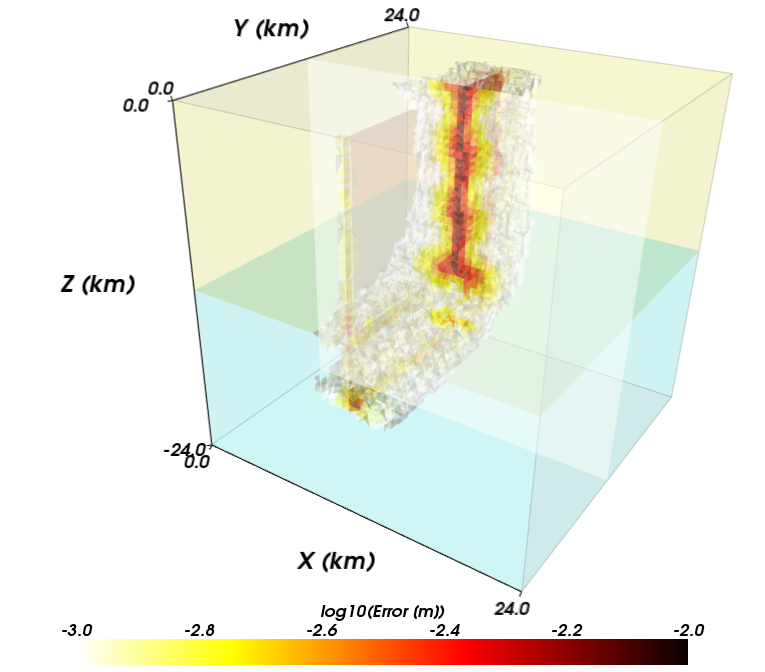
\includegraphics[scale=0.33]{benchmarks/strikeslip/figs/error_tet4_0500m}
\par\end{centering}

\caption{Local error for strike-slip benchmark problem with tetrahedral cells
and linear basis functions with a uniform discretization size of 500
m.\label{fig:benchmark:strikeslip:tet4:500m}}
\end{figure}

\par\end{center}

\noindent \begin{center}
\begin{figure}
\begin{centering}
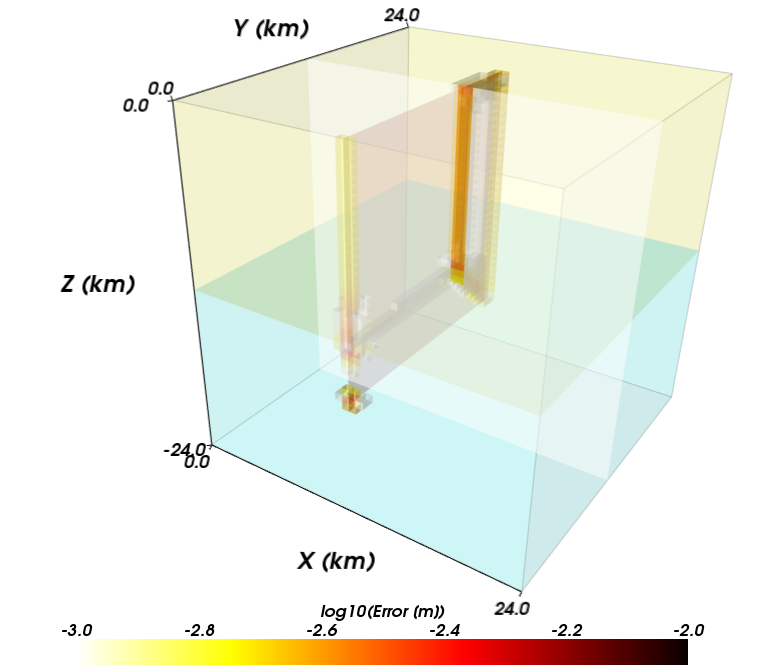
\includegraphics[scale=0.33]{benchmarks/strikeslip/figs/error_hex8_0500m}
\par\end{centering}

\caption{Local error for strike-slip benchmark problem with hexahedral cells
and trilinear basis functions with a uniform discretization size of
500 m.\label{fig:benchmark:strikeslip:hex8:500m}}
\end{figure}

\par\end{center}

\noindent \begin{center}
\begin{figure}[H]
\begin{centering}
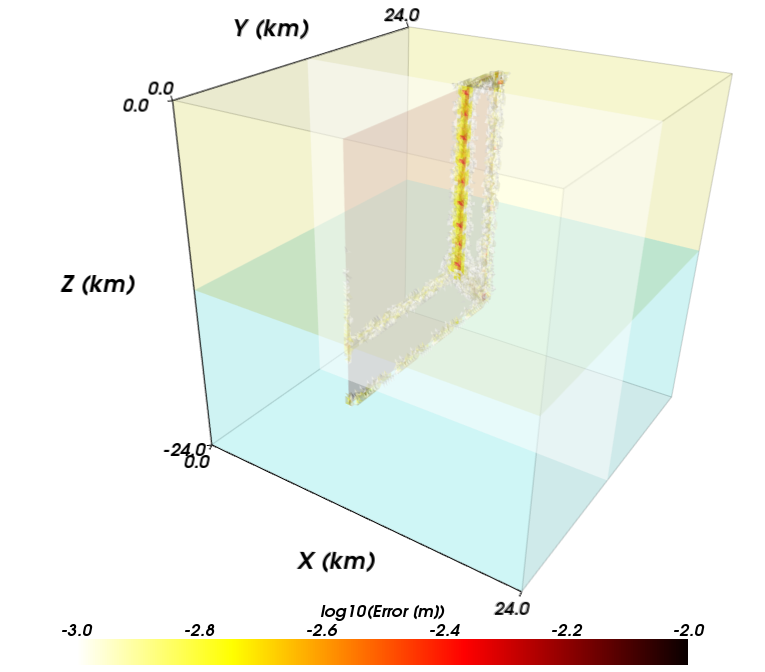
\includegraphics[scale=0.33]{benchmarks/strikeslip/figs/error_tet4_0250m}
\par\end{centering}

\caption{Local error for strike-slip benchmark problem with tetrahedral cells
and linear basis functions with a uniform discretization size of 250
m.\label{fig:benchmark:strikeslip:tet4:250m}}
\end{figure}

\par\end{center}

\noindent \begin{center}
\begin{figure}[H]
\begin{centering}
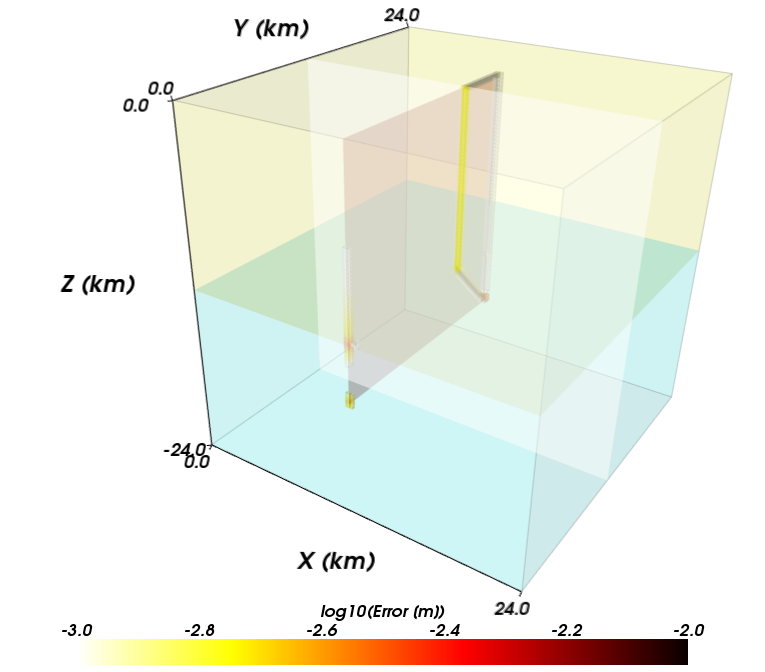
\includegraphics[scale=0.33]{benchmarks/strikeslip/figs/error_hex8_0250m}
\par\end{centering}

\caption{Local error for strike-slip benchmark problem with hexahedral cells
and trilinear basis functions with a uniform discretization size of
250 m.\label{fig:benchmark:strikeslip:hex8:250m}}
\end{figure}

\par\end{center}

\noindent \begin{center}
\begin{figure}[H]
\begin{centering}
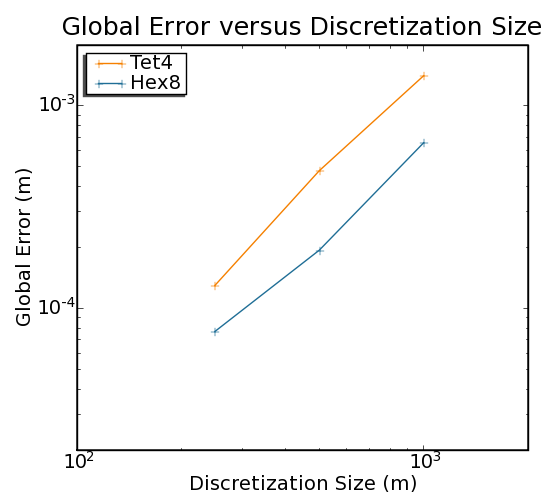
\includegraphics[scale=0.33]{benchmarks/strikeslip/figs/convergence}
\par\end{centering}

\caption{Convergence rate for the strike-slip benchmark problem with tetrahedral
cells and linear basis functions and with hexahedral cells with trilinear
basis functions.\label{fig:benchmark:strikeslip:convergence}}
\end{figure}

\par\end{center}


\subsubsection{Performance}

Figure \ref{fig:benchmark:strikeslip:summary} summarizes the overall
performance of each of the six simulations. Although at a given resolution,
the number of degrees of freedom in the hexahedral and tetrahedral
meshes are the same, the number of cells in the tetrahedral mesh is
about six times greater. However, we use only one integration point
per tetrahedral cell compared to eight for the hexahedral cell. This
leads to approximately the same number of integration points for the
two meshes, but the time required to unpack/pack information for each
cell from the finite-element data structure is greater than the time
required to do the calculation for each quadrature point (which can
take advantage of the very fast, small memory cache in the processor).
As a result, the runtime for the simulations with hexahedral cells
is significantly less than that for the tetrahedral cells at the same
resolution. 

\noindent \begin{center}
\begin{figure}[H]
\begin{centering}
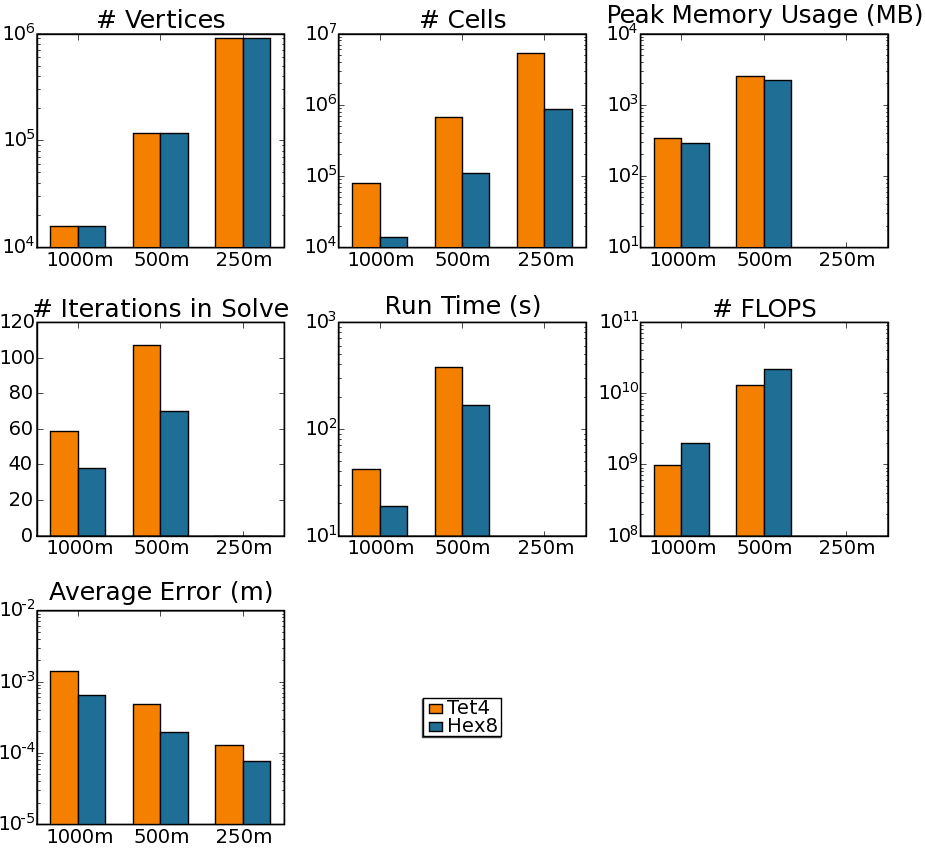
\includegraphics[scale=0.5]{benchmarks/strikeslip/figs/summary}
\par\end{centering}

\caption{Summary of performance of PyLith for the six simulations of the strike-slip
benchmark. For a given discretization size, hexahedral cells with
trilinear basis functions provide greater accuracy with a shorter
runtime compared with tetrahedral cells and linear basis functions.\label{fig:benchmark:strikeslip:summary}}
\end{figure}

\par\end{center}

Figure \vref{fig:benchmark:strikeslip:scaling} compares the runtime
for the benchmark (elastic solution only) at 500 m resolution for
1 to 16 processors. The total runtime is the time required for the
entire simulation, including initialization, distributing the mesh
over the processors, solving the problem in parallel, and writing
the output to VTK files. Some initialization steps, writing the output
to VTK files, and distributing the mesh are essentially serial processes.
For simulations with many time steps these steps will generally occupy
only a fraction of the runtime, and the runtime will be dominated
by the solution of the equations. Figure \ref{fig:benchmark:strikeslip:scaling}
also shows the total time required to form the Jacobian of the system,
form the residual, and solve the system. These steps provide a more
accurate representation of the parallel-performance of the computational
portion of the code and show excellent performance as evident in the
approximately linear slope of 0.7. S linear decrease with a slope
of 1 would indicate strong scaling, which is rarely achieved in real
applications.

\noindent \begin{center}
\begin{figure}[H]
\begin{centering}
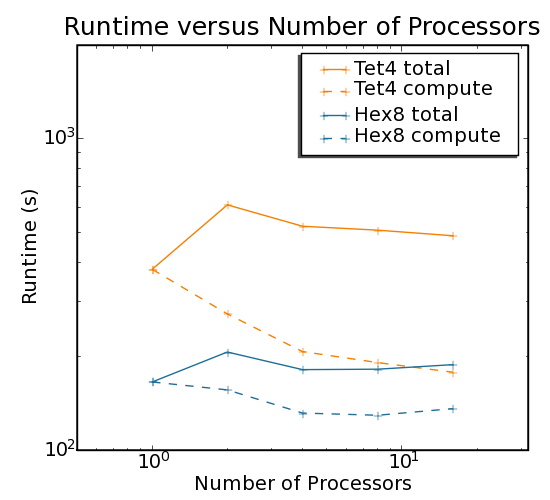
\includegraphics[scale=0.75]{benchmarks/strikeslip/figs/scaling}
\par\end{centering}

\caption{Parallel performance of PyLith for the strike-slip benchmark problem
with tetrahedral cells and linear basis functions with a uniform discretization
size of 500 m. The total runtime (total) and the runtime to compute
the Jacobian and residual and solve the system (compute) are shown.
The compute runtime decreases with a slope of about 0.7; a linear
decrease with a slope of 1 would indicate strong scaling,  which is
rarely achieved in any real application. \label{fig:benchmark:strikeslip:scaling}}
\end{figure}

\par\end{center}
\section{Savage and Prescott Benchmark}
\label{sec:benchmarks:savageprescott}

This benchmark problem computes the viscoelastic (Maxwell) relaxation
of stresses from repeated infinite, strike-slip earthquakes in 3D
without gravity. The files needed to run the benchmark may be found
at \url{https://github.com/geodynamics/pylith_benchmarks/tree/master/quasistatic/sceccrustdeform/savageprescott}.
An analytical solution to this problem is described by Savage and
Prescott \cite{Savage:Prescott:1978}, which provides a simple way
to check our numerical solution. A python utility code is provided
in the utils directory to compute the analytical solution. Although
this problem is actually 2.5D (infinite along-strike), we solve it
using a 3D finite element model.


\subsection{Problem Description}

Figure \ref{fig:benchmark:savageprescott:geometry} shows the geometry
of the problem, as described by \cite{Savage:Prescott:1978}. The
analytical solution describes the surface deformation due to repeated
earthquakes on an infinite strike-slip fault embedded in an elastic
layer overlying a Maxwell viscoelastic half-space. The upper portion
of the fault (red in the figure) is locked between earthquakes, while
the lower portion (blue in the figure) creeps at plate velocity. At
regular recurrence intervals, the upper portion of the fault abruptly
slips by an amount equal to the plate velocity multiplied by the recurrence
interval, thus 'catching up' with the lower part of the fault.

There are some differences between the analytical solution and our
numerical representation. First, the analytical solution represents
the earthquake cycle as the superposition of uniform fault creep and
an elementary earthquake cycle. Uniform fault creep is simply the
uniform movement of the two plates past each other at plate velocity.
For the elementary earthquake cycle, no slip occurs below the locked
portion of the fault (blue portion in the figure). On the locked (red)
portion of the fault, backslip equal to plate velocity occurs until
the earthquake recurrence interval, at which point abrupt forward
slip occurs. In the finite element solution, we perform the simulation
as described in the figure. Velocity boundary conditions are applied
at the extreme edges of the model to simulate block motion, steady
creep is applied along the blue portion of the fault, and regular
earthquakes are applied along the upper portion of the fault. It takes
several earthquake cycles for the velocity boundary conditions to
approximate the steady flow due to steady block motion, so we would
not expect the analytical and numerical solutions to match until several
earthquakes have occurred. Another difference lies in the dimensions
of the domain. The analytical solution assumes an infinite strike-slip
fault in an elastic layer overlying a Maxwell viscoelastic half-space.
In our finite element model we are restricted to finite dimensions.
We therefore extend the outer boundaries far enough from the region
of interest to approximate boundaries at infinity.

Due to the difficulties in representing solutions in an infinite domain,
there are several meshes that have been tested for this problem. The
simplest meshes have uniform resolution (all cells have equal dimensions);
however, such meshes typically do not provide accurate solutions since
the resolution is too coarse in the region of interest. For that reason,
we also tested meshes where the mesh resolution decreases away from
the center. In the problem description that follows, we will focus
on the hexahedral mesh with finer discretization near the fault
({\tt meshes/hex8\_6.7km.exo.gz}), which provides a good match
with the analytical solution. It will first be necessary to gunzip
this mesh so that it may be used by PyLith.
\begin{description}
\item [Domain] The domain for this mesh spans the region
\begin{gather*}
-1000\leq x\leq1000\ km,\\
-500\leq y\leq500\ km,\\
-400\ km\leq z\leq0.
\end{gather*}
The top (elastic) layer occupies the region $-40\ km\ \leq z\leq0$
and the bottom (viscoelastic) layer occupies the region $-400\ km\ \leq z\leq-40\ km$.
\item [Material~properties] The material is a Poisson solid with a shear
modulus ($\mu$) of 30 GPa. The domain is modeled using an elastic
isotropic material for the top layer and a Maxwell viscoelastic material
for the bottom layer. The bottom layer has a viscosity ($\eta$) of
2.36682e+19 Pa-s, yielding a relaxation time ($2\eta/\mu$) of 50
years.
\item [Fault] The fault is a vertical, left-lateral strike-slip fault.
The strike is parallel to the y-direction at the center of the model:
\begin{gather*}
x=0\ km,\\
-500\leq y\leq500\ km,\\
-40\ km\leq z\leq0.
\end{gather*}
The locked portion of the fault (red section in Figure \ref{fig:benchmark:savageprescott:geometry})
extends from $-20\: km\leq z\leq0$, while the creeping section (blue)
extends from $-40\: km\leq z\leq0$. Along the line where the two
sections coincide ($z=-20\: km$), half of the coseismic displacement
and half of the steady creep is applied (see \texttt{finalslip.spatialdb}
and \texttt{creeprate.spatialdb}).
\item [Boundary~conditions] On the bottom boundary, vertical displacements
are set to zero, while on the y-boundaries the x-displacements are
set to zero. On the x-boundaries, the x-displacements are set to zero,
while constant velocities of +/- 1 cm/yr are applied in the y-direction,
giving a relative plate motion of 2 cm/year.
\item [Discretization] For the nonuniform hexahedral mesh, the resolution
at the outer boundaries is 20 km. An inner region is then put through
one level of refinement, so that near the center of the mesh the resolution
is 6.7 km. All meshes were generated with CUBIT.
\item [Basis~functions] We use trilinear hexahedral cells.
\item [Solution] We compute the surface displacements and compare these
to the analytical solution in Figure \ref{fig:benchmark:savageprescott:solution}.
\end{description}

\begin{figure}[htbp]
  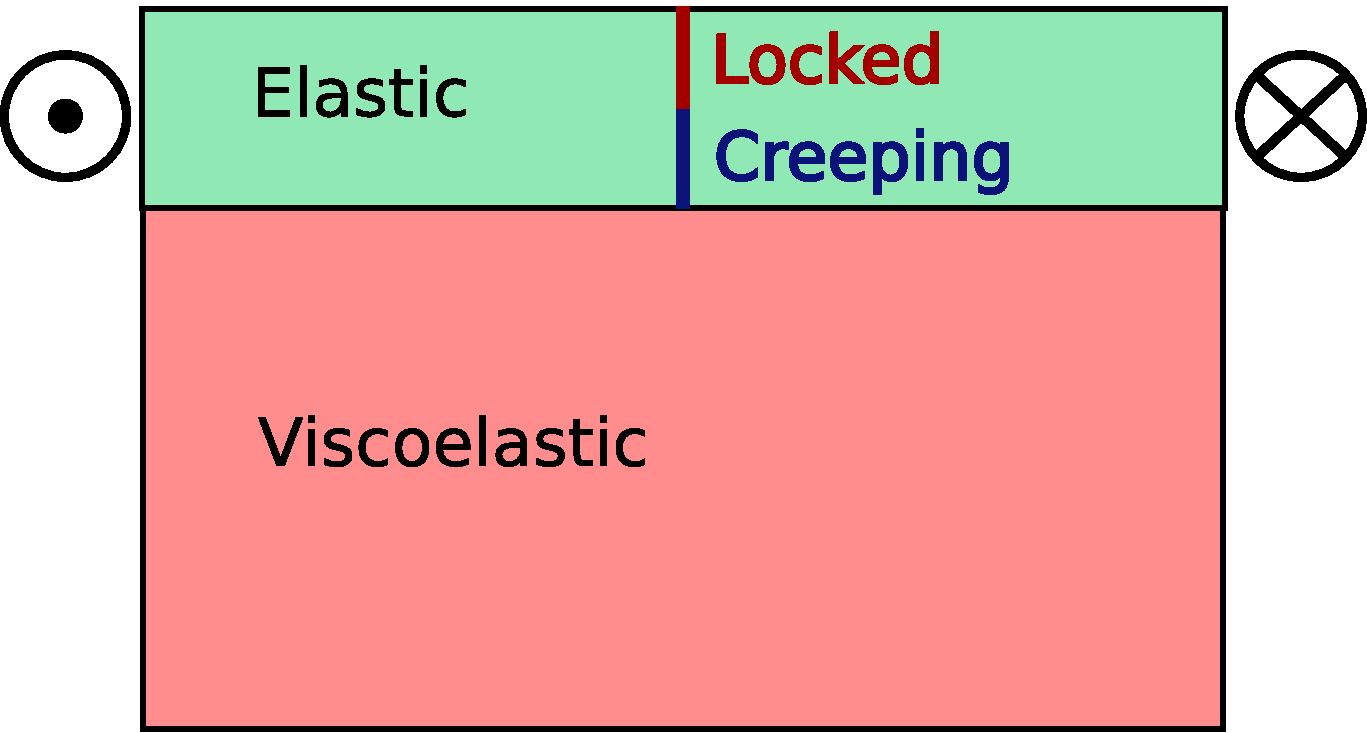
\includegraphics[scale=0.33]{benchmarks/figs/savageprescott_diagram}
  \caption{Problem description for the Savage and Prescott strike-slip
    benchmark problem.}
  \label{fig:benchmark:savageprescott:geometry}
\end{figure}


\subsection{Running the Benchmark}

There are a number of {\tt .cfg} files corresponding to the
different meshes, as well as a {\tt pylithapp.cfg} file defining
parameters common to all problems. Each problem uses four
{\tt .cfg} files: {\tt pylithapp.cfg}, {\tt fieldsplit.cfg}
(algrebraic multigrid preconditioner), a cell-specific file (e.g.,
{\tt hex8.cfg}), and a resolution specific file (e.g.,
hex8\_6.7km.cfg).

\begin{shell}
# If you have not do so already, checkout the benchmarks from the CIG Git repository.
$ git clone https://github.com/geodynamics/pylith_benchmarks.git
# Change to the quasistatic/sceccrustdeform/savageprescott directory.
$ cd quasistatic/sceccrustdeform/savageprescott
# Decompress the gzipped files in the meshes directory.
$ gunzip meshes/*.gz
# Run one of the simulations.
$ pylith hex8.cfg hex8_6.7km.cfg fieldsplit.cfg
\end{shell}

Each simulation uses 10 earthquake cycles of 200 years each,
using a time-step size of 10 years, for a total simulation time of
2000 years. Ground surface output occurs every 10 years, while all
other outputs occur every 50 years.

Once the problem has run, results will be placed in the {\tt output}
directory. These results may be viewed directly using 3-D
visualization software such as ParaView; however, to compare results
to the analytical solution, some postprocessing is required. First,
generate the analytical results by running the {\tt calc\_analytic.py}
script. This will produce files with displacements and velocities
({\tt analytic\_disp.txt} and {\tt analytic\_vel.txt}) in the {\tt
  output} directory that are easy to use with a plotting package, such
as matplotlib or Matlab.


\subsection{Benchmark Results}

Figure \ref{fig:benchmark:savageprescott:solution} shows the computed
surface displacements for the 10th earthquake cycle compared with
the analytical solution. The profile results were obtained as described
above, and then all results (analytical and numerical) were referenced
to the displacements immediately following the last earthquake. We
find very good agreement between the analytical and numerical solutions,
even for meshes with uniform refinement. We have not yet explored
quantitative fits as a function of mesh resolution. For this benchmark,
it is also important to consider the distance of the boundary from
the region of interest. Also note that the agreement between analytical
and numerical solutions is poor for early earthquake cycles, due to
the differences in simulating the problem, as noted above.

\begin{figure}[htbp]
  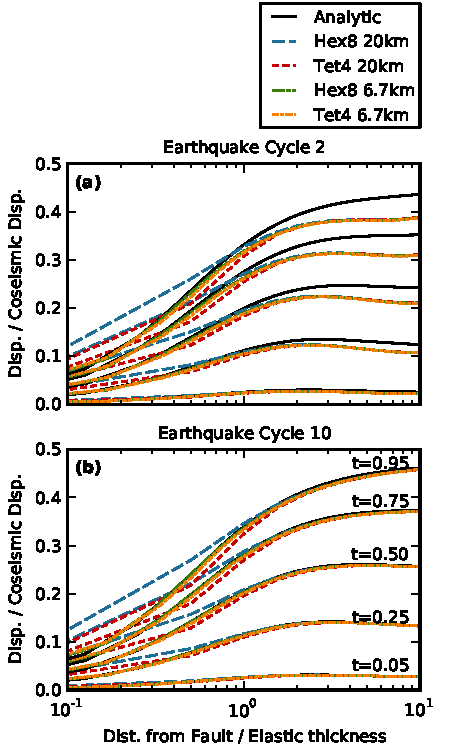
\includegraphics[scale=0.66]{benchmarks/figs/savageprescott_soln_profiles}
  \caption{Displacement profiles perpendicular to the fault for a
    PyLith simulation with hex8 cells and the analytical solution for
    earthquake cycle 10.}
  \label{fig:benchmark:savageprescott:solution}
\end{figure}

% End of file



\section{SCEC Dynamic Rupture Benchmarks}

The SCEC website \url{scecdata.usc.edu/cvws/cgi-bin/cvws.cgi} includes
a graphical user interface for examining the benchmark results. Benchmark
results for PyLith are available for TPV205-2D (horizontal slice through
a vertical strike-slip fault), TPV205 (vertical strike-slip fault
with high and low stress asperities), TPV210-2D (vertical slice through
a 60-degree dipping normal fault), TPV210 (60-degree dipping normal
fault), TPV11, TPV12, TPV13, TPV14-2D and TPV15-2D (horizontal slice
through a verticel strike-slip fault with a branch), TPV14, TPV15,
TPV 24, TPV25 (vertical strike-slip fault with a branch), TPV 16 and
17 (vertical strike-slip fault with spatially heterogeneous initial
tractions), TPV 22 and 23 (vertical strike-slip fault with a stepover),
TPV102 (vertical strike-slip fault with rate-state friction).

The benchmark results indicate that triangular and tetrahedral cells
generate less numerical noise than quadrilateral or hexahedral cells.
The input files in the repository are updated for PyLith v2.0.0, so
you will need to modify them if you use another version of PyLith.

\chapter{Extending PyLith}
\label{cha:extending}

One of the powerful features of using the Pyre framework in PyLith is
the ability to extend the functionality of the software without
altering any of the PyLith code. Any of the components can be replaced
with other compatible components. You are already familiar with this
feature from running the examples; when you set the spatial database
to \object{UniformDB}, \object{SimpleDB}, or \object{SCECCVMH} you are
switching between different compatible components for a spatial
database facility. Modifying the governing equations to include other
physical processes requires changing the data structures associated
with the solution and altering the PyLith code.

In this section we provide examples of how to extend PyLith for components
that users will most likely want to replace with their own custom
versions. You will need a familiarity with Python, Makefiles, and
C++ to write your own components. The primary steps in constructing
a component to extend PyLith's functionality include:
\begin{enumerate}
\item Setting up the source files for the component or set of components
  based on the templates.
\item Edit the Python source file (\filename{.py}) for the component.
  \begin{enumerate}
  \item Define the user-specified properties and facilities.
  \item Transfer the user-specified data from the Python object to the corresponding
    C++ object via calls to the SWIG interface object.
  \end{enumerate}
\item Edit the C++ header (\filename{.hh}) and implementation files (\filename{.cc})
  for the component.
  \begin{enumerate}
  \item Implement the methods required to satisfy the interface definition
    of the component.
  \item Implement the desired functionality of the component in C++.
  \end{enumerate}
\item Edit the SWIG interface files (\texttt{.i}) that provide the glue
  between Python and C++.
\item Edit the Python source file that tests the functionality of the component.
\item Run configure, build, install, and run the tests of the component.
\end{enumerate}

\section{Spatial Databases}
\label{sec:extending:spatialdata:databases}

PyLith provides several types of spatial databases that can be used
for specification of parameters associated with boundary conditions,
earthquake ruptures, and physical properties. In this example we demonstrate
how to provide a spatial database, UniformVelModel, for specifying
elastic properties. The source files are included in the source for
the spatialdata package in the \filename{templates/spatialdb} directory.
The \filename{README} file in \filename{templates/spatialdb} provides
detailed instructions for the various steps involved, and the source
files contain numerous comments to help guide you through the customization
process. 

The \object{UniformVelModel} component provides uniform physical
properties: P-wave speed, S-wave speed, and density. Although this is
a rather trivial specification of physical properties that could be
easily done using a UniformDB, this example demonstrates how to create
a user-defined component that matches the requirements of a spatial
database for elastic physical properties. Adding additional physical
properties is simply a matter of including some additional values in
the spatial database. Furthermore, in cases where we are constructing
a spatial database for a seismic velocity model, the data points are
geovreferenced. With our uniform physical properties we do not need to
worry about any differences in coordinate systems between our seismic
velocity model and points at which the model is queried. However, in
many cases we do, so we illustrate this functionality by using a
geographic projection as the coordinate system in our example.

Using a top-down approach, the first step is to determine what
information the user will need to supply to the component. Is the data
for the spatial database in a file or a series of files? If so, file
names and possible paths to a directory containing files with known
names might be necessary. Are there other parameters that control the
behavior of the component, such as a minimum shear wave speed? In our
example the user supplies values for the P-wave speed, S-wave speed,
and density.  The user-supplied parameters become Pyre properties and
facilities in the Python source file. Because our user supplied
parameters are floating point values with dimensions, we create
dimensional properties vs, vp, and density. In addition to defining the properties of the
component, we also need to transfer these properties to the C++ object
that does the real work. This is done by calling the C++
\texttt{vs()}, \texttt{vp()}, and \texttt{density()} accessor
functions that are accessible via the Python module created by SWIG.

In the C++ object we must implement the functions that are required
by the spatial database interface. These functions are listed near
the beginning of the UniformVelModel class definition at the top of
the C++ header file, \filename{UniformVelModel.hh}. The C++ object also
includes the accessor functions that allow us to set the P-wave speed,
S-wave speed, and density values to the user-specified values in the
Python object. Additional information, such as a file name, parameters
defined as data structures, etc., would be set via similar accessor
functions. You can also add additional functions and data structures
to the C++ class to provide the necessary operations and functionality
of the spatial database. 

In \object{SimpleDB} we use a separate class to read in the spatial
database and yet another class to perform the actual query. In our
example, the C++ object also creates and stores the UTM zone 10
geographic projection for the seismic velocity model. When the spatial
database gets a query for physical properties, we transform the
coordinates of the query point from its coordinate system to the
coordinate system of our seismic velocity model.

In order to use SWIG to create the Python module that allows us to
call C++ from Python, we use a ``main'' SWIG interface file
(\filename{spatialdbcontrib.i} in this case) and then one for each
object (\filename{UniformVelModel.i} in this case). This greatly
simplifies keeping the Python module synchronized with the C++ and
Python code. The \filename{UniformVelModel.i} SWIG file is nearly
identical to the corresponding C++ header file.  There are a few
differences, as noted in the comments within the file.  Copying and
pasting the C++ header file and then doing a little cleanup is a very
quick and easy way to construct a SWIG interface file for a C++
object. Because very little changes from SWIG module to SWIG module,
it is usually easiest to construct the ``main'' SWIG interface by
copying and customizing an existing one.

Once the Python, C++, and SWIG interface files are complete, we are
ready to build the module. The \filename{Makefile.am} file defines how
to compile and link the C++ library and generate the Python module via
SWIG. The \filename{configure.ac} file contains the information used
to build a configure script. The configure script checks to make sure
it can find all of the tools needed to build the component (C++
compiler, Python, installed spatial database package, etc.). See the
README file for detailed instructions on how to generate the configure
script, and build and install the component.

We recommend constructing tests of the component to insure that it is
functioning properly before attempting to use it in an application.
The \filename{tests} directory within \filename{templates/spatialdb}
contains a Python script, \filename{testcontrib.py}, that runs the
tests of the UniformVelModel component defined in
\filename{TestUniformVelModel.py}.  Normally, one would want to test
each function individually to isolate errors and create C++ tests as
well as the Python tests included here.  In our rather simple example,
we simply test the overall functionality of the component. For
examples of thorough testing, see the spatialdata and PyLith source
code.

Once you have built, installed, and tested the UniformVelModel, it
is time to use it in a simple example. Because the seismic velocity
model uses geovreferenced coordinates, our example must also use geovreferenced
coordinates. The dislocation example in the PyLith \filename{examples/twocells/twotet4-geoproj}
directory uses UTM zone 11 coordinates. The spatial database package
will transform the coordinates between the two projections as defined
in the UniformVelModel \texttt{query()} function. The dislocation
example uses the SCEC CVM-H seismic velocity model. In order to replace
the SCEC CVM-H seismic velocity with our uniform velocity model, in
\filename{pylithapp.cfg}
\begin{cfg}
# Replace these two lines
<f>db_properties</f> = spatialdata.spatialdb.SCECCVMH
<p>db_properties.data_dir</p> = /home/john/data/sceccvm-h/vx53/bin
# with
<f>db_properties</f> = spatialdata.spatialdb.contrib.UniformVelModel
\end{cfg}
When you run the dislocation example, the \filename{dislocation-statevars\_info.vtk}
file should vreflect the use of physical properties from the uniform
seismic velocity with $\mu=1.69\times10^{10}\mathrm{Pa}$, $\lambda=1.6825\times10^{10}\mathrm{Pa}$,
and $\rho=2500\mathrm{kg/m^{3}}$.


\section{Bulk Constitutive Models}
\label{sec:extending:materials}

PyLith includes several linearly elastic and inelastic bulk
constitutive models for 2D and 3D problems. In this example, we
demonstrate how to extend PyLith by adding your own bulk constitutive
model. We reimplement the 2D plane strain constitutive model while
adding the current strain and stress tensors as state variables. This
constitutive model, \object{PlaneStrainState}, is not particularly
useful, but it illustrates the basic steps involved in creating a bulk
constitutive model with state variables. The source files are included
with the main PyLith source code in the \filename{templates/materials}
directory. The \filename{README} file in
\filename{templates/materials} provides detailed instructions for the
various steps, and the source files contain numerous comments to guide
you through the customization process.

In contrast to our previous example of creating a customized spatial
database, which involved gathering user-specified parameters via the
Pyre framework, there are no user-defined parameters for bulk
constitutive models. The specification of the physical properties and
state variables associated with the constitutive model is handled
directly in the C++ code. As a result, the Python object for the
constitutive model component is very simple, and customization is
limited to simply changing the names of objects and labels.

The properties and state variables used in the bulk constitutive model
are set using arguments to the constructor of the C++ \object{ElasticMaterial}
object. We define a number of constants at the top of the C++ file
and use the \object{Metadata} object to define the properties and
state variables. The C++ object for the bulk constitutive component
includes a number of functions that implement elasticity behavior
of a bulk material as well as several utility routines:
\begin{description}
\item [{\texttt{\_dbToProperties()}}] Computes the physical properties
  used in the constitutive model equations from the physical properties
  supplied in spatial databases.
\item [{\texttt{\_nondimProperties()}}] Nondimensionalizes the physical
  properties used in the constitutive model equations.
\item [{\texttt{\_dimProperties()}}] Dimensionalizes the physical properties
  used in the constitutive model equations.
\item [{\texttt{\_stableTimeStepImplicit()}}] Computes the stable time
  step for implicit time stepping in quasi-static simulations given
  the current state (strain, stress, and state variables).
\item [{\texttt{\_calcDensity()}}] Computes the density given the physical
  properties and state variables. In most cases density is a physical
  property used in the constitutive equations, so this is a trivial
  function in those cases.
\item [{\texttt{\_calcStress()}}] Computes the stress tensor given the
  physical properties, state variables, total strain, initial stress,
  and initial strain.
\item [{\texttt{\_calcElasticConsts()}}] Computes the elastic constants
  given the physical properties, state variables, total strain, initial
  stress, and initial strain.
\item [{\texttt{\_updateStateVars()}}] Updates the state variables given
  the physical properties, total strain, initial stress, and initial
  strain. If a constitutive model does not use state variables, then
  this routine is omitted.
\end{description}
Because it is sometimes convenient to supply physical properties for
a bulk constitutive model that are equivalent but different from the
ones that appear in the constitutive equations (e.g., P-wave speed,
S-wave speed, and density rather then Lame's constants $\mu$, $\lambda,$
and density), each bulk constitutive model component has routines
to convert the physical property parameters and state variables a
user specifies via spatial databases to the physical property properties
and state variables used in the constitutive model equations. In quasi-static
problems, PyLith computes an elastic solution for the first time step
($-\Delta t$ to $t$). This means that for inelastic materials, we
supply two sets of functions for the constitutive behavior: one set
for the initial elastic step and one set for the remainder of the
simulation. See the source code for the inelastic materials in PyLith
for an illustration of an efficient mechanism for doing this.

The SWIG interface files for a bulk constitutive component are set up
in the same manner as in the previous example of creating a customized
spatial database component. The ``main'' SWIG interface file
(\filename{materialscontrib.i} in this case) sets up the Python
module, and the SWIG interface file for the component
(\filename{PlaneStrainState.i} in this case) defines the functions
that should be included in the Python module. Note that because the
C++ \object{ElasticMaterial} object defines a number of pure virtual
methods (which merely specify the interface for the functions and do
not implement default behavior), we must include many protected
functions in the SWIG interface file. If these are omitted, SWIG will
give a warning indicating that some of the functions remain abstract
(i.e., some pure virtual functions defined in the parent class
\object{ElasticMaterial} were not implemented in the child class
\object{PlaneStrainState}), and no constructor is created. When this
happens, you cannot create a \object{PlaneStrainState} Python object.

Once the Python, C++, and SWIG interface files are complete, you are
ready to configure and build the C++ library and Python module for the
component. Edit the \filename{Makefile.am} file as necessary, then
generate the configure script, run \filename{configure}, and then
build and install the library and module (see the \filename{README}
file for detailed instructions).

Because most functionality of the bulk constitutive model component is
at the C++ level, properly constructed unit tests for the
\object{component} should include tests for both the C++ code and
Python code. The C++ unit tests can be quite complex, and it is best
to examine those used for the bulk constitutive models included with
PyLith. In this example we create the Python unit tests to verify that
we can create a \object{PlaneStrainState} Python object and call some
of the simple underlying C++ functions.  The source files are in the
\filename{templates/materials/tests} directory.  The
\filename{testcontrib.py} Python script runs the tests defined in
\filename{TestPlaneStrainState.py}.

Once you have built, installed, and tested the \object{PlaneStrainState}
component, it is time to use it in a simple example. You can try using
it in any of the 2D examples. For the examples in \filename{examples/twocells/twoquad4},
in \filename{pylithapp.cfg}
\begin{cfg}
# Replace
<f>material</f> = pylith.materials.ElasticPlaneStrain
# with
<f>material</f> = pylith.materials.contrib.PlaneStrainState
\end{cfg}
or simply add the command line argument
\commandline{-{}-timedependent.homogeneous.material=pylith.materials.contrib.PlaneStrainState}.
when running any of the 2D examples. The output should remain
identical, but you should see the \object{PlaneStrainState} object
listed in the information written to stdout.


\section{Fault Constitutive Models}
\label{sec:extending:fault}

PyLith includes two of the most widely used fault constitutive models,
but there are a wide range of models that have been proposed to explain
earthquake source processes. In this example, we demonstrate how to
extend PyLith by adding your own fault constitutive model. We implement
a linear viscous fault constitutive model wherein the perturbation
in the coefficient of friction is linearly proportional to the slip
rate. This constitutive model, \object{ViscousFriction}, is not particularly
useful, but it illustrates the basic steps involved in creating a
fault constitutive model. The source files are included with the main
PyLith source code in the \filename{templates/friction} directory. The
\filename{README} file in \filename{templates/friction} provides detailed
instructions for the various steps, and the source files contain numerous
comments to guide you through the customization process.

Similar to our previous example of creating a customized bulk constitutive
model, the parameters are defined in the C++ code, not in the Pyre
framework. As a result, the Python object for the fault constitutive
model component is very simple and customization is limited to simply
changing the names of objects and labels.

The properties and state variables used in the fault constitutive
model are set using arguments to the constructor of the C++ \object{FrictionModel}
object, analogous to the \object{ElasticMaterial} object for bulk
constitutive models. In fact, both types of constitutive models used
the same underlying C++ object (\object{Metadata::ParamDescription})
to store the description of the parameters and state variables. We
define a number of constants at the top of the C++ file and use the
\object{Metadata} object to define the properties and state variables.
The C++ object for the fault constitutive component includes a number
of functions that implement friction as well as several utility routines:
\begin{description}
\item [{\texttt{\_dbToProperties()}}] Computes the physical properties
  used in the constitutive model equations from the physical properties
  supplied in spatial databases.
\item [{\texttt{\_nondimProperties()}}] Nondimensionalizes the physical
  properties used in the constitutive model equations.
\item [{\texttt{\_dimProperties()}}] Dimensionalizes the physical properties
  used in the constitutive model equations.
\item [{\texttt{\_dbToStateVars()}}] Computes the initial state variables
  used in the constitutive model equations from the initial values supplied
  in spatial databases.
\item [{\texttt{\_nondimStateVars()}}] Nondimensionalizes the state variables
  used in the constitutive model equations.
\item [{\texttt{\_dimStateVars()}}] Dimensionalizes the state variables
  used in the constitutive model equations.
\item [{\texttt{\_calcFriction()}}] Computes the friction stress given
  the physical properties, state variables, slip, slip rate, and normal
  traction.
\item [{\texttt{\_updateStateVars()}}] Updates the state variables given
  the physical properties, slip, slip rate, and normal traction.
\end{description}
If a constitutive model does not use state variables, then the state
variable routines are omitted. 

Because it is sometimes convenient to supply physical properties for a
fault constitutive model that are equivalent but different from the
ones that appear in the constitutive equations, each fault
constitutive model component has routines to convert the physical
property parameters and state variables a user specifies via spatial
databases to the physical property properties and state variables used
in the constitutive model equations.

The SWIG interface files for a fault constitutive component are set up
in the same manner as in the previous examples of creating a bulk
constitutive model or a customized spatial database component. The
``main'' SWIG interface file (\filename{frictioncontrib.i} in this
case) sets up the Python module, and the SWIG interface file for the
component (\filename{ViscousFriction.i} in this case) defines the
functions that should be included in the Python module. Note that
because the C++ \object{FrictionModel} object defines a number of pure
virtual methods (which merely specify the interface for the functions
and do not implement default behavior), we must include many protected
functions in the SWIG interface file. If these are omitted, SWIG will
give a warning indicating that some of the functions remain abstract
(i.e., some pure virtual functions defined in the parent class
\object{FrictionModel} were not implemented in the child class
\object{ViscousFriction}), and no constructor is created. When this
happens, you cannot create a \object{ViscousFriction} Python object.

Once the Python, C++, and SWIG interface files are complete, you are
ready to configure and build the C++ library and Python module for the
component. Edit the \filename{Makefile.am} file as necessary, then
generate the configure script, run \filename{configure}, and then
build and install the library and module (see the \filename{README}
file for detailed instructions).

Because most functionality of the fault constitutive model component
is at the C++ level, properly constructed unit tests for the
\object{component} should include tests for both the C++ code and
Python code. The C++ unit tests can be quite complex, and it is best
to examine those used for the fault constitutive models included with
PyLith. In this example we create the Python unit tests to verify that
we can create a \object{ViscousFriction} Python object and call some
of the simple underlying C++ functions.  The source files are in the
\filename{templates/friction/tests} directory.  The
\filename{testcontrib.py} Python script runs the tests defined in
\filename{TestViscousFriction.py}.

Once you have built, installed, and tested the \object{ViscousFriction}
component, it is time to use it in a simple example. You can try using
it in any of the 2D or 3D examples. For the examples in \filename{examples/bar\_shearwave/quad4,}
in \filename{shearwave\_staticfriction.cfg}
\begin{cfg}
# Replace
<f>friction</f> = pylith.friction.StaticFriction
# with
<f>friction</f> = pylith.friction.contrib.ViscousFriction
\end{cfg}
or simply add the command line argument
\commandline{-{}-timedependent.interfaces.fault.friction=pylith.friction.contrib.ViscousFriction}
when running any of the friction examples. You will also need to
supply a corresponding spatial database with the physical properties
for the viscous friction constitutive model.


\appendix
%dummy comment inserted by tex2lyx to ensure that this paragraph is not empty

\chapter{\label{cha:Glossary}Glossary}


\section{Pyre}
\begin{description}
\item [{component}] Basic building block of a Pyre application. A component
may be built-up from smaller building blocks, where simple data types
are called properties and data structures and objects are called facilities.
In general a component is a specific implementation of the functionality
of a facility. For example, SimpleDB is a specific implementation
of the spatial database facility. A component is generally composed
of a Python object and a C++ object, although either one may be missing.
We nearly always use the naming convention such that for an object
called Foo the Python object is in file Foo.py, the C++ class definition
is in Foo.hh, inline C++ functions are in foo.icc, the C++ class implementation
is in Foo.cc, and the SWIG interface file that glues the C++ and Python
code together is in Foo.i.
\item [{facility}] Complex data type (object or data structure) building
block of a component. See component.
\item [{property}] Simple data type (string, integer, real number, or boolean
value) parameter for a component.
\end{description}

\section{DMPlex}
\begin{description}
\item [{DMPlex}] The plex construction is a representation of the topology
of the finite element mesh based upon a covering relation. For example,
segments are covered by their endpoints, faces by their bounding edges,
etc. Geometry is absent from the plex, and is represented instead
by a  field with the coordinates of the vertices. Meshes can also
be understood as directed acyclic graphs, where we call the constituents
points and arrows.
\item [{mesh}] A finite element mesh, used to partition space and provide
support for the basis functions.
\item [{cell}] The highest dimensional elements of a mesh, or mesh entities
of codimension zero.
\item [{vertex}] The zero dimensional mesh elements.
\item [{face}] Mesh elements that separate cells, or mesh entities of codimension
one.
\item [{field}] A parallel section which can be completed, or made consistent,
across process boundaries. These are used to represent continuum fields.
\item [{section}] These objects associate values in vectors to points (vertices,
 edges, faces, and cells) in a mesh. The section describes the offset
 into the vector along with the number of values associated with each
point.
\item [{dimension}] The topological dimension of the mesh, meaning the
cell dimension. It can also mean the dimension of the space in which
the mesh is embedded, but this is properly the embedding dimension.
\item [{fiber\ dimension}] Dimension of the space associated with the
field. For example, the scalar field has a fiber dimension of 1 and
a vector field has a fiber displacement equal to the dimension of
the mesh.
\item [{cohesive\ cell}] A zero volume cell inserted between any two cells
which shared a fault face. They are prisms with a fault face as the
base.
\item [{cone}] The set of entities which cover any entity in a mesh. For
example, the cone of a triangle is its three edges.
\item [{support}] The set of mesh entities which are covered by any entity
in a mesh. For example, the support of a triangle is the two tetrahedra
it separates.
\end{description}



\chapter{\label{cha:components}PyLith and Spatialdata Components}

The name of the component is followed by the full path name and description.
The full path name is used when setting a component to a facility
in a \texttt{.cfg} file or with command line arguments.


\section{Application components}
\begin{description}
\item [{\texttt{PyLithApp}}] \texttt{pylith.apps.PyLithApp}\\
PyLith application.
\end{description}

\subsection{Problem Components}
\begin{description}
\item [{\texttt{TimeDependent}}] \texttt{pylith.problems.TimeDependent}\\
Time-dependent problem.
\item [{\texttt{GreensFns}}] \texttt{pylith.problems.GreensFns}\\
Static Green's function problem with slip impulses.
\item [{\texttt{Implicit}}] \texttt{pylith.problems.Implicit}\\
Implicit time stepping for static and quasi-static simulations with
infinitesimal strains.
\item [{\texttt{ImplicitLgDeform}}] \texttt{pylith.problems.ImplicitLgDeform}\\
Implicit time stepping for static and quasi-static simulations including
the effects of rigid body motion and small strains.
\item [{\texttt{Explicit}}] \texttt{pylith.problems.Explicit}\\
Explicit time stepping for dynamic simulations with a lumped system
Jacobian matrix.
\item [{\texttt{ExplicitLgDeform}}] \texttt{pylith.problems.ExplicitLgDeform}\\
Explicit time stepping for dynamic simulations including the effects
of rigid body motion and small strains with a lumped system Jacobian
matrix.
\item [{\texttt{ExplicitTri3}}] \texttt{pylith.problems.ExplicitTri3}\\
Optimized elasticity formulation for linear triangular cells and one
quadrature point for explicit time stepping in dynamic simulations.
\item [{\texttt{ExplicitTet4}}] \texttt{pylith.problems.ExplicitTet4}\\
Optimized elasticity formulation for linear tetrahedral cells and
one quadrature point for explicit time stepping in dynamic simulations.
\item [{\texttt{SolverLinear}}] \texttt{pylith.problems.SolverLinear}\\
Linear PETSc solver (KSP).
\item [{\texttt{SolverNonlinear}}] \texttt{pylith.problems.SolverNonlinear}\\
Nonlinear PETSc solver (SNES).
\item [{\texttt{SolverLumped}}] \texttt{pylith.problems.SolverLumped}\\
Built-in simple, optimized solver for solving systems with a lumped
Jacobian.
\item [{\texttt{TimeStepUniform}}] \texttt{pylith.problems.TimeStepUniform}\\
Uniform time stepping.
\item [{\texttt{TimeStepAdapt}}] \texttt{pylith.problems.TimeStepAdapt}\\
Adaptive time stepping (time step selected based on estimated stable
time step).
\item [{\texttt{TimeStepUser}}] \texttt{pylith.problems.TimeStepUser}\\
User defined time stepping (variable time step set by user).
\end{description}

\subsection{Utility Components}
\begin{description}
\item [{\texttt{NullComponent}}] \texttt{pylith.utils.NullComponent}\\
Null component used to set a facility to an empty value.
\item [{\texttt{EventLogger}}] \texttt{pylith.utils.EventLogger}\\
PETSc event logger.
\item [{\texttt{VTKDataReader}}] \texttt{pylith.utils.VTKDataReader}\\
Data reader for VTK files, requires TVTK Enthought package available
from \texttt{}~\\
\texttt{https://github.com/enthought/mayavi.}
\end{description}

\subsection{Topology Components}
\begin{description}
\item [{\texttt{Distributor}}] \texttt{pylith.topology.Distributor}\\
Distributor of mesh among processors in parallel simulations.
\item [{\texttt{JacobianViewer}}] \texttt{pylith.topology.JacobianViewer}\\
Viewer for writing Jacobian sparse matrix to file.
\item [{\texttt{MeshGenerator}}] \texttt{pylith.topology.MeshGenerator}\\
Mesh generator/importer.
\item [{\texttt{MeshImporter}}] \texttt{pylith.topology.MeshImporter}\\
Mesh importer/reader.
\item [{\texttt{MeshRefiner}}] \texttt{pylith.topology.MeshRefiner}\\
Default (null) mesh vrefinement object that does not vrefine the mesh.
\item [{\texttt{RefineUniform}}] \texttt{pylith.topology.RefineUniform}\\
Uniform global mesh vrefinement.
\item [{\texttt{ReverseCuthillMcKee}}] \texttt{pylith.topology.ReverseCuthillMcKee}\\
Object used to manage reordering cells and vertices using the reverse
Cuthill-McKee algorithm.
\end{description}

\subsection{Material Components}
\begin{description}
\item [{\texttt{ElasticStrain1D}}] \texttt{pylith.materials.ElasticStrain1D}\\
Linearly elastic 1D bulk constitutive model with 1D strain ($\epsilon_{yy}=\epsilon_{zz}=0$).
\item [{\texttt{ElasticStress1D}}] \texttt{pylith.materials.ElasticStress1D}\\
Linearly elastic 1D bulk constitutive model with 1D stress ($\sigma_{yy}=\sigma_{zz}=0$).
\item [{\texttt{ElasticPlaneStrain}}] \texttt{pylith.materials.ElasticPlaneStrain}\\
Linearly elastic 2D bulk constitutive model with plane strain ($\epsilon_{zz}=0$).
\item [{\texttt{ElasticPlaneStress}}] \texttt{pylith.materials.ElasticPlaneStress}\\
Linearly elastic 2D bulk constitutive model with plane stress ($\sigma_{zz}=0$).
\item [{\texttt{ElasticIsotropic3D}}] \texttt{pylith.materials.ElasticIsotropic3D}\\
Linearly elastic 3D bulk constitutive model.
\item [{\texttt{MaxwellIsotropic3D}}] \texttt{pylith.materials.MaxwellIsotropic3D}\\
Linear Maxwell viscoelastic bulk constitutive model.
\item [{\texttt{MaxwellPlaneStrain}}] \texttt{pylith.materials.MaxwellPlaneStrain}\\
Linear Maxwell viscoelastic bulk constitutive model for plane strain
problems.
\item [{\texttt{GenMaxwellIsotropic3D}}] \texttt{pylith.materials.GenMaxwellIsotropic3D}\\
Generalized Maxwell viscoelastic bulk constitutive model.
\item [{\texttt{GenMaxwellPlaneStrain}}] \texttt{pylith.materials.GenMaxwellPlaneStrain}\\
Generalized Maxwell viscoelastic bulk constitutive model for plane
strain problems.
\item [{\texttt{PowerLaw3D}}] \texttt{pylith.materials.PowerLaw3D}\\
Power-law viscoelastic bulk constitutive model.
\item [{\texttt{PowerLawPlaneStrain}}] \texttt{pylith.materials.PowerLawPlaneStrain}\\
Power-law viscoelastic bulk constitutive model for plane strain problems.
\item [{\texttt{DruckerPrage3D}}] \texttt{pylith.materials.DruckerPrager3D}\\
Drucker-Prager elastoplastic bulk constitutive model.
\item [{\texttt{DruckerPragePlaneStrain}}] \texttt{pylith.materials.DruckerPragerPlaneStrain}\\
Drucker-Prager elastoplastic bulk constitutive model for plane strain
problems.
\item [{\texttt{Homogeneous}}] \texttt{pylith.materials.Homogeneous}\\
Container with a single bulk material.
\end{description}

\subsection{Boundary Condition Components}
\begin{description}
\item [{\texttt{AbsorbingDampers}}] \texttt{pylith.bc.AbsorbingDampers}\\
Absorbing boundary condition using simple dashpots.
\item [{\texttt{DirichletBC}}] \texttt{pylith.bc.DirichletBC}\\
Dirichlet (prescribed displacements) boundary condition for a set
of points.
\item [{\texttt{DirichletBoundary}}] \texttt{pylith.bc.DirichletBoundary}\\
Dirichlet (prescribed displacements) boundary condition for a set
of points associated with a boundary surface.
\item [{\texttt{Neumann}}] \texttt{pylith.bc.Neumann}\\
Neumann (traction) boundary conditions applied to a boundary surface.
\item [{\texttt{PointForce}}] \texttt{pylith.bc.PointForce}\\
Point forces applied to a set of vertices.
\item [{\texttt{ZeroDispDB}}] \texttt{pylith.bc.ZeroDispDB}\\
Specialized UniformDB with uniform zero displacements at all degrees
of freedom.
\end{description}

\subsection{Fault Components}
\begin{description}
\item [{\texttt{FaultCohesiveKin}}] \texttt{pylith.faults.FaultCohesiveKin}\\
Fault surface with kinematic (prescribed) slip implemented using cohesive
elements.
\item [{\texttt{FaultCohesiveDyn}}] \texttt{pylith.faults.FaultCohesiveDyn}\\
Fault surface with dynamic (friction) slip implemented using cohesive
elements.
\item [{\texttt{FaultCohesiveImpulses}}] \texttt{pylith.faults.FaultCohesiveImpulses}\\
Fault surface with Green's functions slip impulses implemented using
cohesive elements.
\item [{\texttt{EqKinSrc}}] \texttt{pylith.faults.EqKinSrc}\\
Kinematic (prescribed) slip earthquake rupture.
\item [{\texttt{SingleRupture}}] \texttt{pylith.faults.SingleRupture}\\
Container with one kinematic earthquake rupture.
\item [{\texttt{StepSlipFn}}] \texttt{pylith.faults.StepSlipFn}\\
Step function slip-time function.
\item [{\texttt{ConstRateSlipFn}}] \texttt{pylith.faults.ConstRateSlipFn}\\
Constant slip rate slip-time function.
\item [{\texttt{BruneSlipFn}}] \texttt{pylith.faults.BruneSlipFn}\\
Slip-time function where slip rate is equal to Brune's far-field slip
function.
\item [{\texttt{LiuCosSlipFn}}] \texttt{pylith.faults.LiuCosSlipFn}\\
Slip-time function composed of three sine/cosine functions. Similar
to Brune's far-field time function but with more abrupt termination
of slip.
\item [{\texttt{TimeHistorySlipFn}}] \texttt{pylith.faults.TimeHistorySlipFn}\\
Slip-time function with a user-defined slip time function.
\item [{\texttt{TractPerturbation}}] \texttt{pylith.faults.TractPerturbation}\\
Prescribed traction perturbation applied to fault with constitituve
model in additional to tractions from deformation (generally used
to nucleate a rupture).
\end{description}

\subsection{Friction Components}
\begin{description}
\item [{\texttt{StaticFriction}}] \texttt{pylith.friction.StaticFriction}\\
Static friction fault constitutive model.
\item [{\texttt{SlipWeakening}}] \texttt{pylith.friction.SlipWeakening}\\
Linear slip-weakening friction fault constitutive model.
\item [{\texttt{RateStateAgeing}}] \texttt{pylith.friction.RateStateAgeing}\\
Dieterich-Ruina rate and state friction with ageing law state variable
evolution.
\item [{\texttt{TimeWeakening}}] \texttt{pylith.friction.TimeWeakening}\\
Linear time-weakening friction fault constitutive model.
\end{description}

\subsection{Discretization Components}
\begin{description}
\item [{\texttt{FIATLagrange}}] \texttt{pylith.feassemble.FIATLagrange}\\
Finite-element basis functions and quadrature rules for a Lagrange
vreference finite-element cell (point, line, quadrilateral, or hexahedron)
using FIAT. The basis functions are constructed from the tensor produce
of 1D Lagrange vreference cells.
\item [{\texttt{FIATSimplex}}] \texttt{pylith.feassemble.FIATSimplex}\\
Finite-element basis functions and quadrature rules for a simplex
finite-element cell (point, line, triangle, or tetrahedron) using
FIAT.
\end{description}

\subsection{Output Components}
\begin{description}
\item [{\texttt{MeshIOAscii}}] \texttt{pylith.meshio.MeshIOAscii}\\
Reader for simple mesh ASCII files.
\item [{\texttt{MeshIOCubit}}] \texttt{pylith.meshio.MeshIOCubit}\\
Reader for CUBIT Exodus files.
\item [{\texttt{MeshIOLagrit}}] \texttt{pylith.meshio.MeshIOLagrit}\\
Reader for LaGriT GMV/Pset files.
\item [{\texttt{OutputManager}}] \texttt{pylith.meshio.OutputManager}\\
General output manager for mesh information and data.
\item [{\texttt{OutputSoln}}] \texttt{pylith.meshio.OutputSoln}\\
Output manager for solution data.
\item [{\texttt{OutputSolnSubset}}] \texttt{pylith.meshio.OutputSolnSubset}\\
Output manager for solution data over a submesh.
\item [{\texttt{OutputSolnPoints}}] \texttt{pylith.meshio.OutputSolnPoints}\\
Output manager for solution data at arbitrary points in the domain.
\item [{\texttt{OutputDirichlet}}] \texttt{pylith.meshio.OutputDirichlet}\\
Output manager for Dirichlet boundary condition information over a
submesh.
\item [{\texttt{OutputNeumann}}] \texttt{pylith.meshio.OutputNeumann}\\
Output manager for Neumann boundary condition information over a submesh.
\item [{\texttt{OutputFaultKin}}] \texttt{pylith.meshio.OutputFaultKin}\\
Output manager for fault with kinematic (prescribed) earthquake ruptures.
\item [{\texttt{OutputFaultDyn}}] \texttt{pylith.meshio.OutputFaultDyn}\\
Output manager for fault with dynamic (friction) earthquake ruptures.
\item [{\texttt{OutputFaultImpulses}}] \texttt{pylith.meshio.OutputFaultImpulses}\\
Output manager for fault with static slip impulses.
\item [{\texttt{OutputMatElastic}}] \texttt{pylith.meshio.OutputMatElastic}\\
Output manager for bulk constitutive models for elasticity.
\item [{\texttt{SingleOutput}}] \texttt{pylith.meshio.SingleOutput}\\
Container with single output manger.
\item [{\texttt{PointsList}}] \texttt{pylith.meshio.PointsList}\\
Manager for text file container points for \texttt{OutputSolnPoints}.
\item [{\texttt{DataWriterVTK}}] \texttt{pylith.meshio.DataWriterVTK}\\
Writer for output to VTK files.
\item [{\texttt{DataWriterHDF5}}] \texttt{pylith.meshio.DataWriterHDF5}\\
Writer for output to HDF5 files.
\item [{\texttt{DataWriterHDF5Ext}}] \texttt{pylith.meshio.DataWriterHDF5Ext}\\
Writer for output to HDF5 files with datasets written to external
raw binary files.
\item [{\texttt{CellFilterAvg}}] \texttt{pylith.meshio.CellFilterAvg}\\
Filter that averages information over quadrature points of cells.
\item [{\texttt{VertexFilterVecNorm}}] \texttt{pylith.meshio.VertexFilterVecNorm}\\
Filter that computes magnitude of vectors for vertex fields.
\end{description}

\section{Spatialdata Components}


\subsection{Coordinate System Components}
\begin{description}
\item [{\texttt{CSCart}}] \texttt{spatialdata.geocoords.CSCart}\\
Cartesian coordinate system (0D, 1D, 2D, or 3D).
\item [{\texttt{CSGeo}}] \texttt{spatialdata.geocoords.CSGeo}\\
Geographic coordinate system.
\item [{\texttt{CSGeoProj}}] \texttt{spatialdata.geocoords.CSGeoProj}\\
Coordinate system associated with a geographic projection.
\item [{\texttt{CSGeoLocalCart}}] \texttt{spatialdata.geocoords.CSGeoLocalCart}\\
Local, geovreferenced Cartesian coordinate system.
\item [{\texttt{Projector}}] \texttt{spatialdata.geocoords.Projector}\\
Geographic projection.
\item [{\texttt{Converter}}] \texttt{spatialdata.geocoords.Converter}\\
Converter for transforming coordinates of points from one coordinate
system to another.
\end{description}

\subsection{Spatial database Components}
\begin{description}
\item [{\texttt{UniformDB}}] \texttt{spatialdata.spatialdb.UniformDB}\\
Spatial database with uniform values.
\item [{\texttt{SimpleDB}}] \texttt{spatialdata.spatialdb.SimpleDB}\\
Simple spatial database that defines fields using a point cloud. Values
are determined using a nearest neighbor search or linear interpolation
in 0D, 1D, 2D, or 3D.
\item [{\texttt{SimpleIOAscii}}] \texttt{spatialdata.spatialdb.SimpleIOAscii}\\
Reader/writer for simple spatial database files.
\item [{\texttt{SCECCVMH}}] \texttt{spatialdata.spatialdb.SCECCVMH}\\
Spatial database interface to the SCEC CVM-H (seismic velocity model).
\item [{\texttt{CompositeDB}}] \texttt{spatialdata.spatialdb.CompositeDB}\\
Spatial database composed from multiple other spatial databases.
\item [{\texttt{TimeHistory}}] \texttt{spatialdata.spatialdb.TimeHistory}\\
Time history for temporal variations of a parameter.
\item [{\texttt{GravityField}}] \texttt{spatialdata.spatialdb.GravityField}\\
Spatial database providing vector for body forces associated with
gravity.
\end{description}

\subsection{Nondimensionalization components}
\begin{description}
\item [{\texttt{Nondimensional}}] \texttt{spatialdata.units.Nondimensional}\\
Nondimensionalization of length, time, and pressure scales.
\item [{\texttt{NondimensionalElasticDynamic}}] \texttt{spatialdata.units.NondimensionalElasticDynamic}\\
Nondimensionalization of scales for dynamic problems.
\item [{\texttt{NondimensionalElasticQuasistatic}}] \texttt{spatialdata.units.NondimensionalElasticQuasistatic}\\
Nondimensionalization of scales for quasi-static problems.\end{description}


\chapter{File Formats}

\section{Input Files}

PyLith gathers its input from several different types of files. All of
these area ASCII files and can include comment lines that begin with
'\#'. Note that the placement of comments is restricted to certain
locations in some files (see the discussion of each file format for
more information).

% Required input files
\subsection{xx.coord}

The \filename{xx.coord} file contains the coordinates of all of the
vertices in the finite-element mesh.

\begin{figure}
  \begin{center}
\begin{verbatim}
# File containing vertices of the finite-element mesh.
#
# Comment lines begin with '#'
#
# First, specify units of coordinates.
#
coord_unit = km
#
#
# Now specify the coordinates of each vertex.
#
# Columns:
#   (1) Vertex number
#   (2) X coordinate
#   (3) Y coordinate
#   (4) Z coordinate
#
# Note: No comments are allowed within the list of vertex coordinates
#
1  0.000000e+00  0.000000e+00  0.000000e+00
2  1.000000e+00  0.000000e+00  0.000000e+00
3  0.000000e+00  2.000000e+00  0.000000e+00
4  1.000000e+00  2.000000e+00  3.000000e+00
\end{verbatim}
    \ldots
    \caption{Format of \filename{xx.coord} files.}
  \end{center}
\end{figure}

\subsection{xx.connect}

The \filename{xx.connect} file contains the finite-element mesh
topology and material type information, including the element type,
material type, and the lists of vertices for each element.

\begin{figure}
  \begin{center}
\begin{verbatim}
# File containing finite-element mesh topology and material type
# information.
#
# Comment lines begin with '#'
#
# Columns:
#   (1) Element number
#   (2) Element type
#        1 = Linear hexahedron (8 vertices)
#        2 = Linear hexahedron with 1 set of collapsed vertices
#            (7 vertices) [NOT IMPLEMENTED]
#        3 = Linear hexahedron with 2 sets of collapsed vertices
#           (6 vertices) [NOT IMPLEMENTED]
#        4 = Linear hexahedron with 4 vertices collapsed to a point
#            (5 vertices) [NOT IMPLEMENTED]
#        5 = Linear tetrahedron (4 vertices)
#        6 = Quadratix hexahedron (20 vertices) [NOT IMPLEMENTED]
#        7 = Quadratic hexahedron with 3 vertices along one edge 
#            collapsed to a point (18 vertices) [NOT IMPLEMENTED]
#        8 = Quadratic hexahedron with 3 sets of collapsed vertices
#            (15 vertices) [NOT IMPLEMENTED]
#        9 = Quadratic hexahedron with 9 vertices collapsed to a point
#            (13 vertices) [NOT IMPLEMENTED]
#       10 = Quadratic tetrahedron (10 vertices)  [NOT IMPLEMENTED]
#   (3) Material type, numbered consecutively beginning with '1'
#   (4) Infinite element flag, required but not currently implemented
#        0 = only valid value
#   (5)+ Vertices in the element, identified by vertex number
#
# Note: No comments are allowed within the mesh information.
#
1  5  1  0  2911  2865  2886  2864
2  5  2  0   843  3999  4029  3926
3  5  1  0   684  8975  2346  6219
\end{verbatim}
    \ldots
    \caption{Format of \filename{xx.connect} files.}
  \end{center}
\end{figure}  

\subsection{xx.bc}

The \filename{xx.bc} file specifies the displacements, velocity,
and/or forces applied to vertices on the boundaries.

\begin{figure}[htbp]
  \begin{center}
\begin{verbatim}
# File containing boundary conditions at vertices.
#
# Comment lines begin with '#'
#
# First, specify units of coordinates for each type of boundary
# conditon.  All three are required even if they are not all used.
#
displacement_units = m
velocity_units = m/s
force_units = newton
#
#
# Boundary conditions applied to vertices. You must specify a flag and
# value for each degree of freedom, even if some are free.
#
# Columns:
#   (1) Vertex number
#   (2) Boundary condition flag for x DOF
#   (3) Boundary condition flag for y DOF
#   (4) Boundary condition flag for z DOF
#       0 = Free
#       1 = Fixed displacement
#       2 = Constant velocity
#       3 = Constant force
#       A 2 or more digit code may be used for the boundary condition
#       flag.  If used, the the final digit refers to the condition
#       type as defined above, while the beginning digit(s) refer to
#       the time history to be used.
#   (5) Boundary condition value for x DOF
#   (6) Boundary condition value for y DOF
#   (7) Boundary condition value for z DOF
1   0  1  0  0.0000e+00  0.0000e+00  0.0000e+00
3   0  1  0  0.0000e+00  0.0000e+00  0.0000e+00
12  0  1  0  0.0000e+00  0.0000e+00  0.0000e+00
\end{verbatim}
    \ldots
    \caption{Format of \filename{xx.bc} files.}
  \end{center}
\end{figure}

\subsection{xx.time}

The \filename{xx.time} file specifies the time stepping parameters for
the simulation.

\begin{warning}
  The convergence criteria depend on the type of solution and material
  models. The time step for a linear elastic problem is much different
  than that for a nonlinear or time-dependent problem.
\end{warning}

\begin{figure}
  \begin{center}
\begin{verbatim}
# File containing time stepping parameters.
#
# Comment lines begin with '#'
#
# First, specify units used in values with dimensions of time.
#
time_units = year
#
#
# Time stepping parameters are given in groups. The elastic solution
# corresponds to group 0 and must always be defined. Although some of
# the parameters do not have any meaning for the elastic solution,
# they must be present anyway.
#
# Columns:
#   (1) Time step group number (=0 for elastic solution).
#   (2) The number of time steps in the group (=1 for elastic solution).
#   (3) Time step size (given in units of time_units).
#   (4) Amount of implicitness. Real dimensionless parameter that
#       ranges from 0.0 (fully explicit) to 1.0 (fully implicit). The
#       value is generally set to 0.5.
#   (5) Maximum number of equilibrium iterations before stiffness
#       matrix is reformed.
#   (6) Number of time steps between initial reformation of stiffness
#       matrix.
#       &lt;0 Indicates that reformation should occur only for the first
#          step in each time step group.
#       =0 Indicates that reformation should never occur.
#   (7) Large deformation solution flag (only Linear strain is
#       presently available).
#       0 = Linear strain 
#       1 = Large strain but use only linear contribution to the
#           stiffness matrix (sometimes results in better convergence)
#       2 = Large strain and use nonlinear contribution to the
#           stiffness matrix
#   (8) Convergence tolerance for displacements (dimensionless value)
#   (9) Convergence tolerance for forces (dimensionless value)
#   (10) Convergence tolerance for energy (dimensionless value)
#   (11) Maximum number of equilibrium iterations
#
  0   1  0.0  5.0e-01 1001   4  0  1.0e+00  1.0e+0  1.0e+00 1
  1 100  0.1  5.0e-01 1001  -1  0  1.0e+00  1.0e+0  1.0e+00 1
\end{verbatim}
    \ldots
    \caption{Format of \filename{xx.time} files.}
  \end{center}
\end{figure}

\subsection{xx.prop}

The \filename{xx.prop} file specifies the properties for each material
model in the problem.

\begin{warning}
  The materials must be listed in order according to the material
  number assigned to the elements in \filename{xx.connect}.
\end{warning}

\begin{figure}
  \begin{center}
\begin{verbatim}
# File containing material properties.
#
# Comment lines begin with '#'
#
# The material type and material property values are specified using a
# "keyword = value" syntax. The keywords for the different material
# types are given below. Units for each of the values with dimensions
# must follow the value as illustrated in the examples below.
#
# Materials and keywords:
#   Isotropic linear elastic
#     materialType ='IsotropicLinearElastic'
#     density
#     youngsModulus
#     poissonsRatio
#     endMaterial ='True' (flag indicating end of material)
#   Isotropic linear maxwell viscoelastic
#     materialType ='IsotropicLinearMaxwellViscoelastic'
#     density
#     youngsModulus
#     poissonsRatio
#     viscosity
#     endMaterial ='True' (flag indicating end of material)
#
# Material number 1
materialType = 'IsotropicLinearMaxwellViscoelastic'
density         = 3000.0*kg/m**3
youngsModulus   = 7.5e10*Pa
poissonsRatio   = 0.25
viscosity       = 1.0e+18*Pa*s
endMaterial     = True
# Material number 2
materialType = 'IsotropicLinearElastic'
density         = 3000.0*kg/m**3
youngsModulus   = 7.5e10*Pa
poissonsRatio   = 0.25
endMaterial     = True
# Material number 3
materialType = 'IsotropicLinearMaxwellViscoelastic'
density         = 3000.0*kg/m**3
youngsModulus   = 7.5e10*Pa
poissonsRatio   = 0.25
viscosity       = 1.0e+18*Pa*s
endMaterial     = True
\end{verbatim}
    \ldots
    \caption{Format of \filename{xx.prop} files.}
  \end{center}
\end{figure}

\subsection{xx.statevar}

The \filename{xx.statevar} file specifies which state variables are to
be included in the output of the elastic and time dependent solutions.

\begin{figure}
  \begin{center}
\begin{verbatim}
# File specifying which state variables to output.
#
# Comment lines begin with '#'
#
# State variables occur in groups of 6, corresponding to the number of
# stress/strain components. The present groups are:
#   1-6: Cauchy stress
#   7-12: Total strain
#   13-18: Viscous strain
#   18-24: Plastic strain
#
# Lines:
#   (1) Total accumulated values for the current time step
#   (2) Incremental values (previous to current)
#   (3) Rate values (previous to current)
#
# Columns (per line):
#   (1) Number of state variables to output (0 &le; value &le; 24)
#   (2)+ State variable number to output (1 &le; value &le; 24)
#
    12   1   2   3   4   5   6   7   8   9  10  11  12
    12   1   2   3   4   5   6   7   8   9  10  11  12
    0
\end{verbatim}
    \caption{Format of \filename{xx.statevar} files.}
  \end{center}
\end{figure}


% Optional input files
\subsection{xx.split}

The \filename{xx.split} file specifies the split node information for
modeling dislocations. Dislocations may be used in simulating slip on
faults as well as dike intrusions.

\begin{figure}
  \begin{center}
\begin{verbatim}
# File containing time stepping parameters.
#
# Comment lines begin with '#'
#
# Displacements are specified for each vertex on the fault for each
# element containing the vertex. The displacements on each side of the
# fault or dike should have opposite signs. The displacements
# associated with a single side of the fault for each vertex should be
# the same.
#
# Columns:
#   (1) Element number
#   (2) Vertex number
#   (3) Time history flag
#       0 = Slip only in elastic solution
#      -1 = Slip at constant velocity
#       n = Slip according to load history n (requires xx.hist file)
#   (4) Displacement in x direction
#   (5) Displacement in y direction
#   (6) Displacement in z direction
#
 14886   36    0   0.353500000 0.00000000  -0.353500000
 14887   36    0   0.353500000 0.00000000  -0.353500000
 14896   36    0  -0.353500000 0.00000000   0.353500000
 14981   36    0  -0.353500000 0.00000000   0.353500000
\end{verbatim}
    \ldots
    \caption{Format of \filename{xx.split} files.}
  \end{center}
\end{figure}

\subsection{xx.fuldat}

The \filename{xx.fuldat} file lists the time step numbers at which
full output is desired. The elastic solution (time step 0) is always
included in the output. This file is required for time-dependent
problems.

\begin{figure}
  \begin{center}
\begin{verbatim}
# File containing time steps at which full output is desired.
#
# Comment lines begin with '#'
#
# Note: Time step 0 (elastic solution) is always included in the
# output.
#
# List the time steps, one per line.
#
  10
  50
 100
\end{verbatim}
\ldots
    \caption{Format of \filename{xx.time} files.}
  \end{center}
\end{figure}

\subsection{xx.skew}

The \filename{xx.skew} file specifies local coordinate systems for
nodes. The local coordinate system is specified using two Euler angles
that rotate the local coordinate system to the global coordinate
system.

The applied coordinate rotations apply to all boundary conditions
associated with the nodes listed in the file. These are useful, for
example, if it is desired to apply boundary conditions in a direction
normal or tangential to a side of the mesh when the side does not
align with the global coordinate directions.  Similarly, skew
conditions could be used when specifying slip on a fault that lies at
an angle to the global coordinates.

\begin{figure}
  \begin{center}
\begin{verbatim}
# File containing local nodal coordinates.
#
# Comment lines begin with '#'
#
# First, specify units for rotations.
#
rotation_units = degree
#
#
# Columns:
#   (1) Node number
#   (2) Euler angle for rotation in the x-y plane
#   (3) Euler angle for rotation in the x-z plane
#
68    12.3   4.2
132  -12.3  -4.2
\end{verbatim}
    \ldots
    \caption{Format of \filename{xx.time} files.}
  \end{center}
\end{figure}

\subsection{xx.keyval}

The \filename{xx.keyval} file specifies some simple parameter
settings.

\subsubsection{Winkler forces}

Scaling factors can be applied to Winkler forces, permitting a quick
and easy way to change the density or gravitational acceleration when
Winkler forces are used to simulate gravity.

\paragraph{Quadrature order}

\begin{description}
\item[Full] Quadrature order that should give the exact element
  matrices when the elements are geometrically undistorted.
\item[Reduced] Quadrature order that is one order less than full
  quadrature. Note that for linear tetrahedra full and reduced
  quadrature are equivalent (single integration point).

  \begin{warning}
    Use with caution as reduced quadrature can lead to numerical
    instabilities.
  \end{warning}
  
\item[Selective] Uses Hughes' b-bar formulation to perform reduced
  quadrature on the dilatational parts of the strain-displacement
  matrix.  This can be useful in nearly-incompressible problems.
\end{description}

\paragraph{Prestresses}

Gravitational prestresses can be computed automatically. In such
cases, the elastic properties in the prestress calculation can be set
to uniform values independent of the parameters for any of the
material models. When gravity is being used and prestresses are not
computed automatically, each prestress component can be scaled
independently. Reading prestresses from files is presently disabled.

\begin{figure}
\begin{center}
\begin{verbatim}
# Simple parameter values for various PyLith settings. Defaults are
# listed.
#
# Scaling factors applied to Winkler forces.
#
winklerScaleX = 1.0
winklerScaleY = 1.0
winklerScaleZ = 1.0
#
# Scaling factors applied to differential Winkler forces.
#
winklerSlipScaleX = 1.0
winklerSlipScaleY = 1.0
winklerSlipScaleZ = 1.0
#
# Stress integration and numerical computation of the tangent 
# material matrix.  Default values should be reasonable for most cases.
#
stressTolerance = 1.0e-12*Pa
minimumStrainPerturbation = 1.0e-7
initialStrainPerturbation = 1.0e-1
#
# Specify whether to use the solution from the previous time step as
# the starting guess for the elastic solution in the current time step.
# This feature has not been tested.
#
usePreviousDisplacementFlag = 0
#
# Quadrature order for the problem.
#
quadratureOrder = "Full"
#
# Gravitational acceleration in each direction.
#
gravityX = 0.0*m/(s*s)
gravityY = 0.0*m/(s*s)
gravityZ = 0.0*m/(s*s)
#
# Factors controlling computation of prestresses.
#
prestressAutoCompute = False
prestressAutoChangeElasticProperties = False
prestressAutoComputePoisson = 0.49
prestressAutoComputeYoungs = 1.0e30*Pa
#
prestressScaleXx = 1.0
prestressScaleYy = 1.0
prestressScaleZz = 1.0
prestressScaleXy = 1.0
prestressScaleXz = 1.0
prestressScaleYz = 1.0
#
# Unit numbers used in Fortran code.  These defaults should work for
# most Unix systems, but may be altered if necessary.
#
f77StandardInput = 5
f77StandardOutput = 6
f77FileInput = 10
f77AsciiOutput = 11
f77PlotOutput = 12
f77UcdOutput = 13
\end{verbatim}
  \caption{Format of \filename{xx.keyval} files.}
  \end{center}
\end{figure}

\subsection{xx.hist}

The \filename{xx.hist} files provide time histories for use in
boundary conditions.

\begin{figure}
  \begin{center}
\begin{verbatim}
# File specifying time variation of boundary conditions.
#
# Comment lines begin with '#'
#
# Each time history consists of two or more lines.  The first line
# indicates the number of points in the history and the default load
# value for the history.  Subsequent lines define time/load pairs.
#
# Line 1, column 1: The number of points in the time history
# Line 1, column 2: The value assigned to every point by default
#                   (overridden by values in time history)
# Line 2+, column 1: Time (in seconds) for a given load value
# Line 2+, column 2: Load value at given time
#
      2    1.0
2.84014e+08 0.1
3.15576e+08 0.5
\end{verbatim}
    \caption{Format of \filename{xx.hist} files.}
  \end{center}
\end{figure}

\subsection{xx.wink}

The \filename{xx.wink} file specifies Winkler elements, which may be
used as spring foundations in the simulation of gravity.

\begin{figure}
  \begin{center}
\begin{verbatim}
# File containing Winkler elements.
#
# Comment lines begin with '#'
#
# Flags for the degrees of freedom can have the following values:
#    0 = no Winkler force
#    1 = Winkler force applied at all times
#   -n = Winkler force applied according to load history n
#        (requires xx.hist file)
#
# Columns:
#  (1) Vertex number
#  (2) Flag for DOF in x-direction
#  (3) Flag for DOF in y-direction
#  (4) Flag for DOF in z-direction
#  (5) Magnitude of restoring force for x-direction
#  (6) Magnitude of restoring force for x-direction
#  (7) Magnitude of restoring force for x-direction
#
14  0 -1  0  0.0e+00  1.0e+25  0.0e+00
18  0  1  0  1.0e+20  0.0e+00  0.0e+00
\end{verbatim}
    \ldots
    \caption{Format of \filename{xx.wink} files.}
  \end{center}
\end{figure}



\chapter{\label{cha:materials:alternative:formulations}Alternative Material Model Formulations}


\section{\label{sec:materials:formulations:viscoelastic}Viscoelastic Formulations}

The viscoelastic formulations presently used in PyLith are described
in Section \vref{sec:materials:viscoelastic}. In some cases there
are alternative formulations that may be used in future versions of
PyLith, and those are described here.


\subsection{\label{sub:Effective-Stress-Formulation-Maxwell}Effective Stress
Formulation for a Linear Maxwell Viscoelastic Material}

An alternative technique for solving the equations for a Maxwell viscoelastic
material is based on the effective stress formulation described in
Section \vref{sec:materials:formulation:viscoelastic:effective}. A linear
Maxwell viscoelastic material may be characterized by the same elastic
parameters as an isotropic elastic material ($E$ and $\nu$), as
well as the viscosity, $\eta$. The creep strain increment is
\begin{gather}
\underline{\Delta e}^{C}=\frac{\Delta t\phantom{}^{\tau}\underline{S}}{2\eta}\,\,.\label{eq:D1}
\end{gather}
Therefore,
\begin{gather}
\Delta\overline{e}^{C}=\frac{\Delta t\sqrt{^{\tau}J_{2}^{\prime}}}{\sqrt{3\eta}}=\frac{\Delta t\phantom{}^{\tau}\overline{\sigma}}{3\eta}\,,\,\mathrm{and}\,^{\tau}\gamma=\frac{1}{2\eta}\,\,.\label{eq:D2}
\end{gather}
Substituting Equations \vref{eq:46}, \vref{eq:D1}, and \vref{eq:D2}
into \vref{eq:43}, we obtain
\begin{gather}
^{t+\Delta t}\underline{S}=\frac{1}{a_{E}}\left\{ ^{t+\Delta t}\underline{e}^{\prime}-\frac{\Delta t}{2\eta}\left[(1-\alpha)^{t}\underline{S}+\alpha\phantom{}^{t+\Delta t}\underline{S}\right]\right\} +\underline{S}^{I}\,\,.\label{eq:D3}
\end{gather}
Solving for $^{t+\Delta t}\underline{S}$,
\begin{gather}
^{t+\Delta t}\underline{S}=\frac{1}{a_{E}+\frac{\alpha\Delta t}{2\eta}}\left[^{t+\Delta t}\underline{e}^{\prime}-\frac{\Delta t}{2\eta}(1-\alpha)^{t}\underline{S}+\frac{1+\mathrm{\nu}}{E}\underline{S}^{I}\right]\,\,.\label{eq:D4}
\end{gather}
In this case it is possible to solve directly for the deviatoric stresses,
and the effective stress function approach is not needed. To obtain
the total stress, we simply use
\begin{gather}
^{t+\Delta t}\sigma_{ij}=\phantom{}^{t+\Delta t}S_{ij}+\frac{\mathit{1}}{a_{m}}\left(\,^{t+\Delta t}\theta-\theta^{I}\right)\delta_{ij}+P^{I}\delta_{ij}\,\,.\label{eq:D5}
\end{gather}


To compute the viscoelastic tangent material matrix relating stress
and strain, we need to compute the first term in Equation \vref{eq:58}.
From Equation \vref{eq:D4}, we have
\begin{gather}
\frac{\partial\phantom{}^{t+\Delta t}S_{i}}{\partial\phantom{}^{t+\Delta t}e_{k}^{\prime}}=\frac{\delta_{ik}}{a_{E}+\frac{\alpha\Delta t}{2\eta}}\,\,.\label{eq:D12}
\end{gather}
Using this, along with Equations \vref{eq:58}, \vref{eq:59}, and \vref{eq:60},
the final material matrix relating stress and tensor strain is
\begin{gather}
C_{ij}^{VE}=\frac{1}{3a_{m}}\left[\begin{array}{cccccc}
1 & 1 & 1 & 0 & 0 & 0\\
1 & 1 & 1 & 0 & 0 & 0\\
1 & 1 & 1 & 0 & 0 & 0\\
0 & 0 & 0 & 0 & 0 & 0\\
0 & 0 & 0 & 0 & 0 & 0\\
0 & 0 & 0 & 0 & 0 & 0
\end{array}\right]+\frac{1}{3\left(a_{E}+\frac{\alpha\Delta t}{2\eta}\right)}\left[\begin{array}{cccccc}
2 & -1 & -1 & 0 & 0 & 0\\
-1 & 2 & -1 & 0 & 0 & 0\\
-1 & -1 & 2 & 0 & 0 & 0\\
0 & 0 & 0 & 3 & 0 & 0\\
0 & 0 & 0 & 0 & 3 & 0\\
0 & 0 & 0 & 0 & 0 & 3
\end{array}\right]\,.\label{eq:D13}
\end{gather}
Note that the coefficient of the second matrix approaches $E/3(1+\nu)=1/3a_{E}$
as $\eta$ goes to infinity. To check the results we make sure that
the regular elastic constitutive matrix is obtained for selected terms
in the case where $\eta$ goes to infinity.
\begin{gather}
C_{11}^{E}=\frac{E(1-\nu)}{(1+\nu)(1-2\nu)}\,\,\nonumber \\
C_{12}^{E}=\frac{E\nu}{(1+\nu)(1-2\nu)}\,.\label{eq:D14}\\
C_{44}^{E}=\frac{E}{1+\nu}\,\,\nonumber 
\end{gather}
This is consistent with the regular elasticity matrix, and Equation
\vref{eq:D13} should thus be used when forming the stiffness matrix.
We do not presently use this formulation, but it may be included in
future versions.


\chapter{\label{cha:Analytical-Solns}Analytical Solutions}


\section{\label{sec:TractionProblems}Traction Problems}

Computation of analytical solutions for elastostatic problems over
regular domains is a relatively straightforward procedure. These problems
are typically formulated in terms of a combination of displacement
and traction boundary conditions, and such problems provide a good
test of the code accuracy, as well as specifically testing the implementation
of traction boundary conditions. We present here two simple problems
for this purpose.


\subsection{Solutions Using Polynomial Stress Functions}

Our derivation follows the procedures outlined in Timoshenko and Goodier
\cite{Timoshenko:Goodier:1987}, and we restrict ourselves to two-dimensional
problems. Any problem in elastostatics must satisfy the equilibrium
equations
\begin{gather}
\frac{\partial\sigma_{xx}}{\partial x}+\frac{\partial\sigma_{xy}}{\partial y}+X=0\label{eq:traction:1}\\
\frac{\partial\sigma_{yy}}{\partial y}+\frac{\partial\sigma_{xy}}{\partial x}+Y=0,\nonumber 
\end{gather}
where \textit{X} and \textit{Y} are the body force components in the
\textit{x} and \textit{y} directions, respectively, and the stress
components are given by $\sigma$. In the problems considered here,
we neglect body forces, so \textit{X} and \textit{Y} disappear from
the equilibrium equations. The solution must also satisfy the boundary
conditions, given as surface tractions over the surface of the body.
Finally, the solution must satisfy the conditions of compatibility,
which may be expressed as:
\begin{equation}
\left(\frac{\partial^{2}}{\partial x^{2}}+\frac{\partial^{2}}{\partial y^{2}}\right)\left(\sigma_{xx}+\sigma_{yy}\right)=0.\label{eq:traction:2}
\end{equation}
To compute the displacement field, it is also necessary to specify
displacement boundary conditions.

Equations \vref{eq:traction:1} may be satisfied by taking any function $\phi$
of \textit{x} and \textit{y}, and letting the stress components be
given by the following expressions:
\begin{equation}
\sigma_{xx}=\frac{\partial^{2}\phi}{\partial y^{2}},\;\sigma_{yy}=\frac{\partial^{2}\phi}{\partial x^{2}},\;\sigma_{xy}=-\frac{\partial^{2}\phi}{\partial x\partial y}.\label{eq:traction:3}
\end{equation}
The solution must also satisfy the compatibility equations. Substituting
Equations \vref{eq:traction:3} into Equation \vref{eq:traction:2}, we find that the
stress function $\phi$ must satisfy
\begin{equation}
\frac{\partial^{4}\phi}{\partial x^{4}}+2\frac{\partial^{4}\phi}{\partial x^{2}\partial y^{2}}+\frac{\partial^{4}\phi}{\partial y^{4}}=0.\label{eq:traction:4}
\end{equation}
A relatively easy way to solve a number of problems is to select expressions
for $\phi$ consisting of polynomial functions of \textit{x} and \textit{y}
of second degree or higher. Any polynomial of second or third degree
will satisfy Equation \vref{eq:traction:4}. For polynomials of higher degree,
they must be substituted into Equation \vref{eq:traction:4} to determine what
restrictions must be placed on the solution.


\subsection{\label{sub:Analytical-Constant-Traction}Constant Traction Applied
to a Rectangular Region}

For this problem, a constant normal traction, $\overrightarrow{N}$,
is applied along the positive \textit{x}-edge of the rectangular region
($x=x_{0}$), and roller boundary conditions are applied along the
left and bottom boundaries (\vref{fig:Const-tractions}). Since the
tractions are constant, we assume a second degree polynomial for the
stress function:
\begin{equation}
\phi_{2}=\frac{a_{2}}{2}x^{2}+b_{2}xy+\frac{c_{2}}{2}y^{2}.\label{eq:traction:5}
\end{equation}
This yields the following expressions for the stresses:
\begin{equation}
\sigma_{xx}=\frac{\partial^{2}\phi_{2}}{\partial y^{2}}=c_{2}=N,\;\sigma_{yy}=a_{2}=0,\;\sigma_{xy}=-b_{2}=0.\label{eq:traction:6}
\end{equation}
From Hooke's law, we have:
\begin{equation}
\epsilon_{xx}=\frac{\partial u}{\partial x}=\frac{\left(1-\nu^{2}\right)N}{E},\;\epsilon_{yy}=\frac{\partial v}{\partial y}=\frac{-\nu\left(1+\nu\right)N}{E},\;\epsilon_{xy}=\frac{1}{2}\left(\frac{\partial v}{\partial x}+\frac{\partial u}{\partial y}\right)=0.\label{eq:traction:7}
\end{equation}
The strain components are thus easily obtained from the stress components.

To obtain the displacements, we must integrate Equation \vref{eq:traction:7}
and make use of the displacement boundary conditions. Integrating
the first two of these, we obtain
\begin{equation}
u=\frac{\left(1-\nu^{2}\right)Nx}{E}+f\left(y\right),\; v=\frac{-\nu\left(1+\nu\right)Ny}{E}+f\left(x\right).\label{eq:traction:8}
\end{equation}
Substituting these into the third expression, we obtain
\begin{equation}
\frac{\partial f\left(x\right)}{\partial x}=-\frac{\partial f\left(y\right)}{\partial y},\label{eq:traction:9}
\end{equation}
which means that both $f\left(x\right)$ and $f\left(y\right)$ must
be constant. We solve for these constants using the displacement boundary
conditions along $x=x_{0}$ and $y=y_{0}$. Doing this, we obtain
the following expressions for the displacement components:
\begin{equation}
u=\frac{\left(1-\nu^{2}\right)N}{E}\left(x-x_{0}\right),\; v=\frac{\nu\left(1+\nu\right)N}{E}\left(y_{0}-y\right).\label{eq:traction:10}
\end{equation}


\noindent \begin{center}
\begin{figure}[H]


\caption{\label{fig:Const-tractions}Problem with constant traction boundary
conditions applied along right edge.}


\noindent \centering{}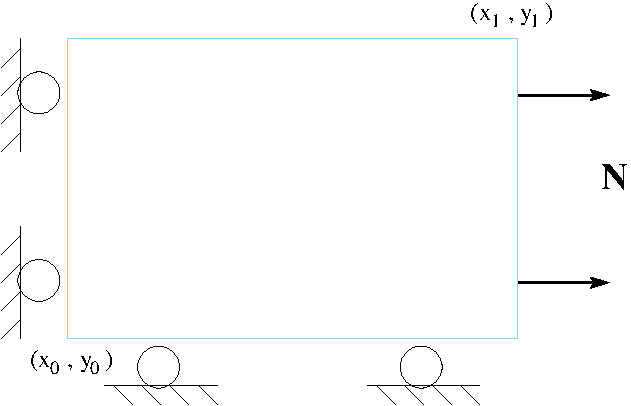
\includegraphics{analyticalsolns/figs/consttract}
\end{figure}

\par\end{center}


\chapter{PyLith Software License}

Copyright (C) 2010-2016 University of California, Davis

Permission is hereby granted, free of charge, to any person obtaining
a copy of this software and associated documentation files (the ``Software''),
to deal in the Software without restriction, including without limitation
the rights to use, copy, modify, merge, publish, distribute, sublicense,
and/or sell copies of the Software, and to permit persons to whom
the Software is furnished to do so, subject to the following conditions:

The above copyright notice and this permission notice shall be included
in all copies or substantial portions of the Software.

THE SOFTWARE IS PROVIDED ``AS IS,'' WITHOUT WARRANTY OF ANY KIND,
EXPRESS OR IMPLIED, INCLUDING BUT NOT LIMITED TO THE WARRANTIES OF
MERCHANTABILITY, FITNESS FOR A PARTICULAR PURPOSE AND NONINFRINGEMENT.
IN NO EVENT SHALL THE AUTHORS OR COPYRIGHT HOLDERS BE LIABLE FOR ANY
CLAIM, DAMAGES OR OTHER LIABILITY, WHETHER IN AN ACTION OF CONTRACT,
TORT OR OTHERWISE, ARISING FROM, OUT OF OR IN CONNECTION WITH THE
SOFTWARE OR THE USE OR OTHER DEALINGS IN THE SOFTWARE. 


\begin{thebibliography}{Bibliography}
\bibitem[Aagaard et al., 2001a]{Aagaard:etal:2001a}Aagaard, B.T.,
J.F. Hall, and T.H. Heaton (2001), Characterization of near-source
ground motions with earthquake simulations, \emph{Earthquake Spectra,
17}(2), 177-207.

\bibitem[Aagaard et al., 2001b]{Aagaard:etal:2001b}Aagaard, B.T.,
T.H. Heaton, and J.F. Hall (2001), Dynamic earthquake ruptures in
the presence of lithostatic normal stresses: Implications for friction
models and heat production, \emph{Bulletin of the Seismological Society
of America, 91}(6), 1765-1796.

\bibitem[Aagaard et al., 2007]{Aagaard:etal:2007}Aagaard, B., C.
Williams, and M. Knepley (2007), PyLith: A finite-element code for
modeling quasi-static and dynamic crustal deformation, \emph{Eos Trans.
AGU, 88}(52), Fall Meet. Suppl., Abstract T21B-0592.

\bibitem[Aagaard et al., 2008]{Aagaard:etal:2008}Aagaard, B., C.
Williams, and M. Knepley (2008), PyLith: A finite-element code for
modeling quasi-static and dynamic crustal deformation, \emph{Eos Trans.
AGU}, \emph{89(}53), Fall Meet. Suppl., Abstract T41A-1925.

\bibitem[Bathe, 1995]{Bathe:1995}Bathe, K.-J. (1995), \textit{Finite-Element
Procedures}, Prentice Hall, Upper Saddle River, New Jersey, 1037 pp.

\bibitem[Ben-Zion and Rice, 1997]{BenZion:Rice:1997}Ben-Zion, Y.
and J.R. Rice (1997), Dynamic simulations of slip on a smooth fault
in an elastic solid, \emph{Journal of Geophysical Research}\textit{,
102}, 17,771\textendash{}17,784.

\bibitem[Brune, 1970]{Brune:1970}Brune, J.N. (1970), Tectonic stress
and spectra of seismic shear waves from earthquakes, \emph{Journal
of Geophysical Research, 75}, 4997-5009.

\bibitem[Courant et al., 1967]{Courant:etal:1967}Courant, R., K.
Friedrichs and H. Lewy (1967), On the Partial Differential Equations
of Mathematical Physics, \textit{IBM Journal of Research and Development},
11(2), 215--234.

\bibitem[Day and Ely, 2002]{Day:Ely:2002}Day, S.M. and G.P. Ely (2002),
Effct of a shallow weak zone on fault rupture: Numerical simulation
of scale-model experiments, \textit{Bull. Seismol. Soc. Am.}, 92(8),
3022-3041, doi: 10.1785/0120010273.

\bibitem[Drucker and Prager, 1952]{Drucker:Prager:1952}Drucker, D.
C. and Prager, W. (1952). Soil mechanics and plastic analysis for
limit design, \textit{Quarterly of Applied Mathematics}, \textit{10},
157\textendash{}165.

\bibitem[Liu et al., 2006]{Liu:etal:2006}Liu, P., R.J. Archuleta,
S.H. Hartzell (2006), Prediction of broadband ground-motion time histories:
Hybrid low/high-frequency method with correlated random source parameters,
\textit{Bull. Seismol. Soc. Am., 96}, 2118-2130.

\bibitem[Kaneko et al., 2008]{Kaneko:etal:2008}Kaneko, Y., N. Lapusta,
and J.-P. Ampuero (2008), Spectral element modeling of spontaneous
earthquake rupture on rate and state faults: Effect of velocity-strengthening
friction at shallow depths, \textit{Journal of Geophysical Research},\textit{
113}, B09317, doi:10.1029/2007JB005553.

\bibitem[Kaus et al., 2010]{Kaus:etal:2010}Kaus, B. J. P., H. Muhlhaus,
and D. A. May (2010), A stabilization algorithm for geodynamic numerical
simulations with a free surface, \textit{Physics of the Earth and
Planetary Interiors}, \textit{181}, 12-20, doi:10.1016/j.pepi.2010.04.007.

\bibitem[Kirby and Kronenberg, 1987]{Kirby:Kronenberg:1987}Kirby,
S. H. and A. K. Kronenberg (1987), Rheology of the lithosphere: Selected
topics, \textit{Reviews of Geophysics, 25}, 1219-1244.

\bibitem[Knopoff and Ni, 2001]{Knopoff:Ni:2001}Knopoff, L. and X.X.
Ni (2001), Numerical instability at the edge of a dynamic fracture,
\emph{Geophysical Journal International,}\textit{\emph{ }}\textit{147}(3),
1-6, doi: 10.1046/j.1365-246x.2001.01567.x.

\bibitem[Kojic and Bathe, 1987]{Kojic:Bathe:1987}Kojic, M. and K.-J.
Bathe (1987), The `Effective Stress-Function' Algorithm for Thermo-Elasto-Plasticity
and Creep, \emph{Int. J. Num. Meth. Eng}.\emph{, 24}, 1509-1532.

\bibitem[McGarr, 1988]{McGarr:1988}McGarr, A. (1988), On the state
of lithospheric stress in the absence of applied tectonic forces,
\textit{Journal of Geophysical Research}, \textit{93}, 13,609-13,617.

\bibitem[Menke, 1984]{Menke:1984}Menke, W. (1984), \textit{Geophysical
Data Analysis: Discrete Inverse Theory}, Academic Press, Inc., Orlando,
260 pp.

\bibitem[Okada, 1992]{Okada:1992}Okada, Y., Internal deformation
due to shear and tensile faults in a half-space (1992), \textit{Bull.
Seismol. Soc. Am.}, \textit{83}, 1018-1040.

\bibitem[Paterson, 1994]{Paterson:1994}Paterson, W. S. B. (1994),
\textit{The Physics of Glaciers, Third Edition}, Elsevier Science
Ltd., Oxford, 480 pp.

\bibitem[Prentice, 1968]{Prentice:1968}Prentice, J. H, (1968), Dimensional
problem of the power law in rheology, \textit{Nature}, \textit{217},
157.

\bibitem[Savage and Prescott, 1978]{Savage:Prescott:1978}Savage,
J. C. and W. H. Prescott (1978), Asthenosphere readjustment and the
earthquake cycle, \textit{Journal of Geophysical} \textit{Research}\emph{,
83}, 3369-3376.

\bibitem[Taylor, 2003]{Taylor:2003}Taylor, R.L. (2003), `FEAP--A
Finite Element Analysis Program', \textit{Version 7.5 Theory Manual},
154 pp.

\bibitem[Timoshenko and Goodier, 1987]{Timoshenko:Goodier:1987}Timoshenko,
S.P. and J.N. Goodier (1987), \textit{Theory of Elasticity, Third
Edition}, McGraw-Hill, New York, 567 pp.

\bibitem[Williams et al., 2005]{Williams:etal:2005}Williams, C.A.,
B. Aagaard, and M.G. Knepley (2005), Development of software for studying
earthquakes across multiple spatial and temporal scales by coupling
quasi-static and dynamic simulations, \emph{Eos Trans. AGU, 86}(52),
Fall Meet. Suppl., Abstract S53A-1072.

\bibitem[Williams, 2006]{Williams:2006}Williams, C.A. (2006), Development
of a package for modeling stress in the lithosphere, \emph{Eos Trans.
AGU,} \emph{87}(36), Jt. Assem. Suppl., Abstract T24A-01 Invited.

\bibitem[Zienkiewicz and Taylor, 2000]{Zienkiewicz:Taylor:2000}Zienkiewicz,
O.C. and R.L. Taylor (2000), \textit{The Finite Element Method, Fifth
Edition, Volume 2: Solid Mechanics}, Butterworth-Heinemann, Oxford,
459 pp.125\end{thebibliography}

\end{document}
